% ******************************* PhD Thesis Template **************************
% Please have a look at the README.md file for info on how to use the template

\documentclass[a4paper,12pt,times,numbered,print,index,chapter]{Classes/PhDThesisPSnPDF}

% ******************************************************************************
% ******************************* Class Options ********************************
% *********************** See README for more details **************************
% ******************************************************************************

% `a4paper'(The University of Cambridge PhD thesis guidelines recommends a page
% size a4 - default option) or `a5paper': A5 Paper size is also allowed as per
% the Cambridge University Engineering Deparment guidelines for PhD thesis
%
% `11pt' or `12pt'(default): Font Size 10pt is NOT recommended by the University
% guidelines
%
% `oneside' or `twoside'(default): Printing double side (twoside) or single
% side.
%
% `print': Use `print' for print version with appropriate margins and page
% layout. Leaving the options field blank will activate Online version.
%
% `index': For index at the end of the thesis
%
% `draftclassic': For draft mode without loading any images (same as draft in book)
%
% `draft': Special draft mode with line numbers, images, and water mark with
% timestamp and custom text. Position of the text can also be modified.
%
% `abstract': To generate only the title page and abstract page with
% dissertation title and name, to submit to the Student Registry
%
% `chapter`: This option enables only the specified chapter and it's references
%  Useful for review and corrections.
%
% ************************* Custom Page Margins ********************************
%
% `custommargin`: Use `custommargin' in options to activate custom page margins,
% which can be defined in the preamble.tex. Custom margin will override
% print/online margin setup.
%
% *********************** Choosing the Fonts in Class Options ******************
%
% `times' : Times font with math support. (The Cambridge University guidelines
% recommend using times)
%
% `fourier': Utopia Font with Fourier Math font (Font has to be installed)
%            It's a free font.
%
% `customfont': Use `customfont' option in the document class and load the
% package in the preamble.tex
%
% default or leave empty: `Latin Modern' font will be loaded.
%
% ********************** Choosing the Bibliography style ***********************
%
% `authoryear': For author-year citation eg., Krishna (2013)
%
% `numbered': (Default Option) For numbered and sorted citation e.g., [1,5,2]
%
% `custombib': Define your own bibliography style in the `preamble.tex' file.
%              `\RequirePackage[square, sort, numbers, authoryear]{natbib}'.
%              This can be also used to load biblatex instead of natbib
%              (See Preamble)
%
% **************************** Choosing the Page Style *************************
%
% `default (leave empty)': For Page Numbers in Header (Left Even, Right Odd) and
% Chapter Name in Header (Right Even) and Section Name (Left Odd). Blank Footer.
%
% `PageStyleI': Chapter Name next & Page Number on Even Side (Left Even).
% Section Name & Page Number in Header on Odd Side (Right Odd). Footer is empty.
%
% `PageStyleII': Chapter Name on Even Side (Left Even) in Header. Section Number
% and Section Name in Header on Odd Side (Right Odd). Page numbering in footer


% ********************************** Preamble **********************************
% Preamble: Contains packages and user-defined commands and settings
% ******************************************************************************
% ****************************** Custom Margin *********************************

% Add `custommargin' in the document class options to use this section
% Set {innerside margin / outerside margin / topmargin / bottom margin}  and
% other page dimensions
\ifsetCustomMargin
  \RequirePackage[left=37mm,right=30mm,top=35mm,bottom=30mm]{geometry}
  \setFancyHdr % To apply fancy header after geometry package is loaded
\fi

% Add spaces between paragraphs
%\setlength{\parskip}{0.5em}
% Ragged bottom avoids extra whitespaces between paragraphs
\raggedbottom
% To remove the excess top spacing for enumeration, list and description
%\usepackage{enumitem}
%\setlist[enumerate,itemize,description]{topsep=0em}

% *****************************************************************************
% ******************* Fonts (like different typewriter fonts etc.)*************

% Add `customfont' in the document class option to use this section

\ifsetCustomFont
  % Set your custom font here and use `customfont' in options. Leave empty to
  % load computer modern font (default LaTeX font).
  %\RequirePackage{helvet}

  % For use with XeLaTeX
  %  \setmainfont[
  %    Path              = ./libertine/opentype/,
  %    Extension         = .otf,
  %    UprightFont = LinLibertine_R,
  %    BoldFont = LinLibertine_RZ, % Linux Libertine O Regular Semibold
  %    ItalicFont = LinLibertine_RI,
  %    BoldItalicFont = LinLibertine_RZI, % Linux Libertine O Regular Semibold Italic
  %  ]
  %  {libertine}
  %  % load font from system font
  %  \newfontfamily\libertinesystemfont{Linux Libertine O}
\fi

% *****************************************************************************
% **************************** Custom Packages ********************************

% ************************* Algorithms and Pseudocode **************************

%\usepackage{algpseudocode}


% ******************** Captions and Hyperreferencing / URL **********************

% Captions: This makes captions of figures use a boldfaced small font.
%\RequirePackage[small,bf]{caption}

\RequirePackage[labelsep=space,tableposition=top]{caption}
\renewcommand{\figurename}{Fig.} %to support older versions of captions.sty

% ******************** Equation **********************
\usepackage{mathtools}
\DeclarePairedDelimiter\bra{\langle}{\rvert}
\DeclarePairedDelimiter\ket{\lvert}{\rangle}
\DeclarePairedDelimiterX\braket[2]{\langle}{\rangle}{#1 \delimsize\vert #2}
\usepackage{relsize}

% *************************** Graphics and figures *****************************

%\usepackage{rotating}
%\usepackage{wrapfig}

% Uncomment the following two lines to force Latex to place the figure.
% Use [H] when including graphics. Note 'H' instead of 'h'
%\usepackage{float}
%\restylefloat{figure}

% Subcaption package is also available in the sty folder you can use that by
% uncommenting the following line
% This is for people stuck with older versions of texlive
%\usepackage{sty/caption/subcaption}
\usepackage{subcaption}

% ********************************** Tables ************************************
\usepackage{booktabs} % For professional looking tables
\usepackage{multirow}

%\usepackage{multicol}
%\usepackage{longtable}
%\usepackage{tabularx}


% *********************************** SI Units *********************************
\usepackage{siunitx} % use this package module for SI units


% ******************************* Line Spacing *********************************

% Choose linespacing as appropriate. Default is one-half line spacing as per the
% University guidelines

% \doublespacing
% \onehalfspacing
% \singlespacing


% ************************ Formatting / Footnote *******************************

% Don't break enumeration (etc.) across pages in an ugly manner (default 10000)
%\clubpenalty=500
%\widowpenalty=500

%\usepackage[perpage]{footmisc} %Range of footnote options


% *****************************************************************************
% *************************** Bibliography  and References ********************

%\usepackage{cleveref} %Referencing without need to explicitly state fig /table

% Add `custombib' in the document class option to use this section
\ifuseCustomBib
   \RequirePackage[square, sort, numbers, authoryear]{natbib} % CustomBib

% If you would like to use biblatex for your reference management, as opposed to the default `natbibpackage` pass the option `custombib` in the document class. Comment out the previous line to make sure you don't load the natbib package. Uncomment the following lines and specify the location of references.bib file

%\RequirePackage[backend=biber, style=numeric-comp, citestyle=numeric, sorting=nty, natbib=true]{biblatex}
%\bibliography{References/references} %Location of references.bib only for biblatex

\fi

% changes the default name `Bibliography` -> `References'
\renewcommand{\bibname}{References}


% ******************************** Roman Pages *********************************
% The romanpages environment set the page numbering to lowercase roman one
% for the contents and figures lists. It also resets
% page-numbering for the remainder of the dissertation (arabic, starting at 1).

\newenvironment{romanpages}{
  \setcounter{page}{1}
  \renewcommand{\thepage}{\roman{page}}}
{\newpage\renewcommand{\thepage}{\arabic{page}}}


% ******************************************************************************
% ************************* User Defined Commands ******************************
% ******************************************************************************

% *********** To change the name of Table of Contents / LOF and LOT ************

%\renewcommand{\contentsname}{My Table of Contents}
%\renewcommand{\listfigurename}{My List of Figures}
%\renewcommand{\listtablename}{My List of Tables}


% ********************** TOC depth and numbering depth *************************

\setcounter{secnumdepth}{2}
\setcounter{tocdepth}{2}


% ******************************* Nomenclature *********************************

% To change the name of the Nomenclature section, uncomment the following line

%\renewcommand{\nomname}{Symbols}


% ********************************* Appendix ***********************************

% The default value of both \appendixtocname and \appendixpagename is `Appendices'. These names can all be changed via:

%\renewcommand{\appendixtocname}{List of appendices}
%\renewcommand{\appendixname}{Appndx}

% *********************** Configure Draft Mode **********************************

% Uncomment to disable figures in `draftmode'
%\setkeys{Gin}{draft=true}  % set draft to false to enable figures in `draft'

% These options are active only during the draft mode
% Default text is "Draft"
%\SetDraftText{DRAFT}

% Default Watermark location is top. Location (top/bottom)
%\SetDraftWMPosition{bottom}

% Draft Version - default is v1.0
%\SetDraftVersion{v1.1}

% Draft Text grayscale value (should be between 0-black and 1-white)
% Default value is 0.75
%\SetDraftGrayScale{0.8}


% ******************************** Todo Notes **********************************
%% Uncomment the following lines to have todonotes.

%\ifsetDraft
%	\usepackage[colorinlistoftodos]{todonotes}
%	\newcommand{\mynote}[1]{\todo[author=kks32,size=\small,inline,color=green!40]{#1}}
%\else
%	\newcommand{\mynote}[1]{}
%	\newcommand{\listoftodos}{}
%\fi

% Example todo: \mynote{Hey! I have a note}


% ************************ Thesis Information & Meta-data **********************
% Thesis title and author information, refernce file for biblatex
% ************************ Thesis Information & Meta-data **********************
%% The title of the thesis
\title{Writing your PhD thesis in \texorpdfstring{\\ \LaTeX2e}{LaTeX2e}}
%\texorpdfstring is used for PDF metadata. Usage:
%\texorpdfstring{LaTeX_Version}{PDF Version (non-latex)} eg.,
%\texorpdfstring{$sigma$}{sigma}

%% Subtitle (Optional)
\subtitle{Using the CUED template}

%% The full name of the author
\author{Krishna Kumar}

%% Department (eg. Department of Engineering, Maths, Physics)
\dept{Department of Engineering}

%% University and Crest
\university{University of Cambridge}
% Crest minimum should be 30mm.
\crest{
\includegraphics[width=0.2\textwidth]{University_Crest}}
%% Use this crest, if you are using the college crest
%% Crest long miminum should be 65mm
%\crest{
\includegraphics[width=0.45\textwidth]{University_Crest_Long}}

%% College shield [optional] 
% Crest minimum should be 30mm.
%\collegeshield{
\includegraphics[width=0.2\textwidth]{CollegeShields/Kings}}


%% Supervisor (optional)
%% for multiple supervisors, append each supervisor with the \newline command
%\supervisor{\textbf{Prof. A.B. Supervisor\newline
%Prof. C.D. Supervisor\newline
%Prof. E.F. Supervisor\newline
%Prof. G.H. Supervisor}}

%% Supervisor Role (optional) - Supervisor (default) or advisor
% \supervisorrole{\textbf{Supervisors: }}
%% if no title is desired:
% \supervisorrole{}

%% Advisor (optional)
%% for multiple advisors, append each advisor with the \newline command
%\advisor{Advisor 1\newline
%Advisors 2\newline
%Advisor 3\newline
%Advisor 4}
     
%% Advisor Role (optional) - Advisor (default) or leave empty
% \advisorrole{Advisors: }
%% if no title is required
% \advisorrole{}


%% You can redefine the submission text:
% Default as per the University guidelines:
% ``This dissertation is submitted for the degree of''
%\renewcommand{\submissiontext}{change the default text here if needed}

%% Full title of the Degree
\degreetitle{Doctor of Philosophy}

%% College affiliation (optional)
\college{King's College}

%% Submission date
% Default is set as {\monthname[\the\month]\space\the\year}
%\degreedate{September 2014} 

%% Meta information
\subject{LaTeX} \keywords{{LaTeX} {PhD Thesis} {Engineering} {University of
Cambridge}}


% ***************************** Abstract Separate ******************************
% To printout only the titlepage and the abstract with the PhD title and the
% author name for submission to the Student Registry, use the `abstract' option in
% the document class.

\ifdefineAbstract
 \pagestyle{empty}
 \includeonly{Declaration/declaration, Abstract/abstract}
\fi

% ***************************** Chapter Mode ***********************************
% The chapter mode allows user to only print particular chapters with references
% Title, Contents, Frontmatter are disabled by default
% Useful option to review a particular chapter or to send it to supervisior.
% To use choose `chapter' option in the document class

\ifdefineChapter
 \includeonly{NeutrinoPhysics/NeutrinoPhysics}
 \fi

% ************************ User defined ************************
\setcounter{secnumdepth}{3}

% ******************************** Front Matter ********************************
\begin{document}

\frontmatter

\maketitle

% ******************************* Thesis Dedidcation ********************************

\begin{dedication} 

  {\color{red} Dedication could go here...}
%I would like to dedicate this thesis to my loving parents \dots

\end{dedication}


% ******************************* Thesis Declaration ***************************

\begin{declaration}

I hereby declare that except where specific reference is made to the work of 
others, the contents of this dissertation are original and have not been 
submitted in whole or in part for consideration for any other degree or 
qualification in this, or any other university. This dissertation is my own 
work and contains nothing which is the outcome of work done in collaboration 
with others, except as specified in the text and Acknowledgements. This 
dissertation contains fewer than 65,000 words including appendices, 
bibliography, footnotes, tables and equations and has fewer than 150 figures.

% Author and date will be inserted automatically from thesis.tex \author \degreedate

\end{declaration}


\include{Acknowledgements/acknowledgements}
% ************************** Thesis Abstract *****************************
% Use `abstract' as an option in the document class to print only the titlepage and the abstract.
\begin{abstract}

  Neutrino physics is approaching the precision-era, with current and future experiments aiming to perform highly accurate measurements of the parameters which govern the phenomenon of neutrino oscillations.  The ultimate ambition with these results is to search for evidence of CP-violation in the lepton sector, currently hinted at in the world-leading analyses from current experiments, which may explain the dominance of matter over antimatter in the Universe.

  The Deep Underground Neutrino Experiment (DUNE) is a future long-baseline experiment based at Fermi National Accelerator Laboratory (FNAL), with a far detector at the Sanford Underground Research Facility (SURF) and a baseline of 1300~km.  In order to make the required precision measurements, the far detector will utilise a detector consisting of 40~kton liquid argon and an embedded time projection chamber.  This promising technology is still in development and, since each detector module is around a factor 15 larger than any previous experiment employing this design, prototyping the detector and design choices is critical to the success of the experiment.  The 35-ton experiment was constructed for this purpose and will be described in detail in this thesis.  The outcomes of the 35-ton prototype are already influencing DUNE and, following the successes and lessons learned from the experiment, confidence can be taken forward to the next stage of the DUNE programme.

  The main oscillation signal at DUNE will be electron neutrino appearance from the muon neutrino beam.  High-precision studies of these $\nu_e$ interactions requires advanced processing and event reconstruction techniques, particularly in the handling of showering particles such as electrons and photons.  Novel methods developed for the purposes of shower reconstruction in liquid argon are presented with an aim to successfully develop a selection to use in a $\nu_e$ charged-current analysis, and a first-generation selection using the new techniques is presented.
  
\end{abstract}


% *********************** Adding TOC and List of Figures ***********************

\tableofcontents

\listoffigures

\listoftables

% \printnomenclature[space] space can be set as 2em between symbol and description
%\printnomenclature[3em]

\printnomenclature

% ******************************** Main Matter *********************************
\mainmatter

% Introductions
% Target lenth: ~2/3 pages

\graphicspath{{Introduction/Figs/}}

%----------------------------------------------------------------------------------------------------------------------------------------------------------------------------
\chapter{Introduction}\label{chap:Introduction}

The theory of elementary particles, the Standard Model of Particle Physics, is an incredibly successful theory which has stood up to every experimental test since it was first formulated in the 1970s \cite{Glashow1961,Weinberg1967}.  The recent discovery of the Higgs boson at CERN \cite{Aad2012,Chatrchyan2012} was the final missing piece and establishes the Standard Model as \textit{the} theory of physical phenomena at the electroweak scale (up to a few hundred GeV) \cite{Shears2012,Bilenky2015}.

There are however many shortcomings to the theory and further theoretical and experimental work is necessary to advance our understanding of fundamental physics \cite{Ellis2012}.  For example, it ignores gravity and requires a quantised theory of gravity to reconcile it with General Relativity.  The observation of `Dark Matter' and `Dark Energy' in Astrophysics and Cosmology cannot be explained using the known particles in the Standard Model and needs an extension of the theory.  It also offers no convincing explanation of the observed domination of matter over antimatter evident in the Universe, given they were created equally in the Big Bang.  Additionally, there are many unresolved theoretical problems within the Standard Model, evidence of a more fundamental underlying theory which may replace it.  It is for this reason that experiments are hoping to find phenomena which may only be understood `Beyond the Standard Model'.

Neutrinos offer the most promising possibilities of new physics and are currently the subject of a great amount of research \cite{Bilenky2015}.  The observation of neutrino oscillations \cite{SuperKamiokande1998,SNO2002}, along with the associated implication of neutrino mass, represents physics which was not included in, or predicted by, the Standard Model.  In recent years the field of neutrino physics has advanced rapidly and there is currently good understanding of most experimental results.  Open questions remain, such as the origin and nature of neutrino mass, the characteristics of neutrino interactions and the exact features of neutrino mixing, and will define the future of the field for many years to come.  This will be discussed in more detail in Chapter~\ref{chap:NeutrinoPhysics}.  There is also the possibility neutrinos may explain the aforementioned matter-antimatter asymmetry through CP-violation in the lepton sector and may even provide a potential dark matter candidate in the possible sterile neutrino.

Future understanding and discoveries in neutrino physics requires precise measurements from highly sensitive experiments.  The future Deep Underground Neutrino Experiment (DUNE) is such an experiment and will be able to contribute towards many of the unanswered questions in the field.  The DUNE experiment, along with its sensitivities to unexplained phenomena, is the subject of Chapter~\ref{chap:DUNE}.  It will use large quantities of liquid argon in order to make the necessary precision measurements and will be the largest experiment using this technology ever built by an order of magnitude.  In order to ensure the experiment is successful and reaches its physics potential, prototyping the technology and detector design is essential.  The experiences of operating such a prototype, the 35~ton experiment, is discussed in Chapter~\ref{chap:35ton}, and additionally in Chapter~\ref{chap:OnlineMonitoring}.

A major challenge in the design choice of DUNE is the successful and detailed reconstruction of particle interactions necessary to make the required measurements.  This is discussed in depth in Chapter~\ref{chap:LArTPCReconstruction}, with emphasis placed on the difficult task of reconstructing showering particles.  The performance of the reconstruction in the selection of the main signal events for DUNE, and an analysis, at this early stage, of the current status of the DUNE software at meeting its required physics goals, is presented in Chapter~\ref{chap:FDAnalysis}.


% Neutrino physics
% Target length: 30 pages

\graphicspath{{NeutrinoPhysics/Figs/}}

\chapter{Neutrino Physics}\label{chap:NeutrinoPhysics}

This chapter contains an introduction to the field of neutrino physics to provide context for the main work presented in this thesis.  The history of neutrino physics is an interesting story in its own right and provides the foundation for the present and future of the field.  This will be briefly retold in Section \ref{sec:HistoricalContext} and will motivate a discussion of neutrino oscillations in Section \ref{sec:NeutrinoOscillations}.  An overview of the current status of the field and its future is contained in Section \ref{sec:NeutrinoPhysicsStatus}.  As this thesis specifically concerns the DUNE experiment, a brief history and description of liquid argon TPCs is provided in Section \ref{sec:LArTPC} as a basis for future chapters.

%----------------------------------------------------------------------------------------------------------------------------------------------------------------------------
\section{Historical Context}\label{sec:HistoricalContext}

\subsection{Prediction of the Neutrino}\label{NeutrinoPrediction}

The neutrino was first postulated in 1930 by Wolfgang Pauli \cite{Pauli1930} in order to account for an inconsistency in the theory of $\beta$-decay.  In the apparent two-body decay
\begin{equation}
A \rightarrow B + e^-,
\end{equation}
kinematically the electron must be emitted with an energy given by
\begin{equation}\label{eq:BetaDecayEnergy}
E = \left( \frac{m_A^2 - m_B^2 + m_e^2}{2m_A} \right) c^2,
\end{equation}
where $m_{\alpha}$ is the mass of particle $\alpha$.  This energy is fixed given the masses of the particles; it was observed however that the electron energy followed a distribution (Figure~\ref{fig:BetaDecayEnergy}), with Equation \ref{eq:BetaDecayEnergy} giving the maximum permitted energy.  The neutrino was postulated as a third final state particle in order to account for this result and retain energy conservation laws.  Pauli initially called the particle a \textit{neutron} (preempting the name Chadwick was to give his discovered particle in 1932) but his idea was met with much scepticism.  It was Fermi who named the new particle \textit{neutrino} (`little neutral one') when incorporating Pauli's hypothesis into his theory of beta decay \cite{Fermi1934Italian,Fermi1934German,Wilson1968}.  With the huge success and acceptance of this theory, the field of neutrino physics was born.

\begin{figure}
  \centering
  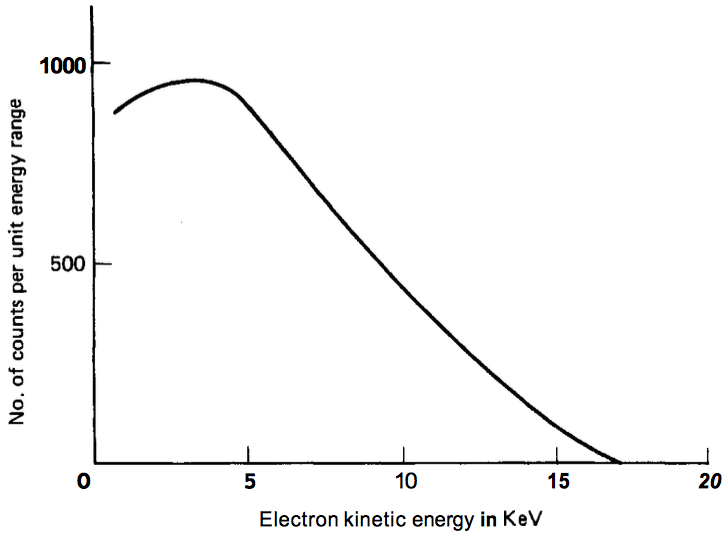
\includegraphics[width=10cm]{ElectronEnergySpectrumBetaDecay.png}
  \caption[Energy spectrum of the electron produced in beta decay.]{Energy spectrum of the electron produced in beta decay \cite{Lewis1970}.}
  \label{fig:BetaDecayEnergy}
\end{figure}

Further indications of the existence of the neutrino were provided by the studies of pion and muon decay by Cecil Powell's group at Bristol in 1947 \cite{Lattes1947-159,Lattes1947-160}.  Topological investigations of the newly discovered $\pi$ meson and its apparent decay into a lighter meson (now known to actually be the muon lepton) appear to hint at the presence of an additional, unknown, daughter particle \cite{Lattes1947-159}.  Furthermore, subsequent studies of the decay of the muons implied a three-body decay involving two unknown final state particles, analogous to the implication of the neutrino in $\beta$-decay by considering the electron energy distribution \cite{Brown1949}.  It seemed a model involving neutrinos could explain these observations and provided more suggestions for the existence of such a particle.

\subsection{Discovery of the Neutrino}\label{NeutrinoDiscovery}

The elegance of Fermi's theory convinced many physicists of the existence of the neutrino but until discovered experimentally it remained a hypothetical `bookkeeping' device.  Given the elusive nature of neutrinos this was not for many years, leading to Pauli famously declaring ``I have done a terrible thing. I have postulated a particle that cannot be detected''.  However, a series of experiments conducted between 1953 and 1956 by Clyde Cowan and Frederick Reines confirmed the hypothesis and were later rewarded with the Nobel Prize in Physics in 1995.  Using the new technology of liquid scintillator detectors \cite{ReinesCowanLiquidScintillation}, they designed an experiment \cite{ReinesCowan1953Proposal} to study the (anti)neutrinos produced in inverse beta decay
\begin{equation}\label{eq:InverseBetaDecay}
  {\bar{\nu}}_e + p \rightarrow e^+ + n
\end{equation}
in the Hanford nuclear reactor in Washington, U.S.A.  Their signal comprised of an initial release of scintillation light when the positron annihilates with an electron, followed a characteristic time later by a gamma ray corresponding to the neutron capture.  The initial results from 1953 \cite{ReinesCowan1953} hinted at an excess over predicted background but the background proved to be much larger than anticipated, mainly due to an underestimation of the effects of cosmic rays.  A second experiment was conducted in 1956, this time 12~m underground and 11~m from the Savannah River reactor in South Carolina.  A neutrino detection rate of 2.9$\pm$0.2 per hour, greater than 20 times the accidental background rate was reported, confirming the previous indications \cite{ReinesCowan1956}.  The experimental discovery of the neutrino was confirmed.  [Bit more description? -- Describe detector, method for detecting positron.]

Ray Davis was also using nuclear reactors to study the interaction rates of neutrinos.  Using a detector comprised of 3000 gallons of carbon tetrachloride (CCl$_4$) also close to the Savannah River reactor, Davis and Harmer searched for the interactions
\begin{equation}\label{eq:DavisAntineutrino}
  \bar{\nu} + \textnormal{Cl}^{37} \rightarrow \textnormal{Ar}^{37} + e^- \hspace{1.5cm} (\bar{\nu} + n \rightarrow p^+ + e^-).
\end{equation}
Since it was known from Reines and Cowan that inverse beta decay
\begin{equation}\label{eq:DavisNeutrino}
  \nu + \textnormal{Cl}^{37} \rightarrow \textnormal{Ar}^{37} + e^- \hspace{1.5cm} (\nu + n \rightarrow p^+ + e^-)
\end{equation}
occurs, this facilitated a comparison between the neutrino and the antineutrino.  They found the interaction shown in Equation \ref{eq:DavisAntineutrino} occurred at a rate less than 20 times that represented in Equation \ref{eq:DavisNeutrino}, implying for the first time a difference between neutrinos and antineutrinos \cite{Davis1959}.  This gave rise to the notion of `lepton number' and its conservation in physical interactions.

It was few years before the next chapter in the history of neutrinos, the discovery of the muon neutrino in 1962 at Brookhaven \cite{Danby1962}.  It was noted the apparently permitted decay
\begin{equation}
\mu^- \not\rightarrow e^- + \gamma
\end{equation}
is never observed, inciting the possibility of two distinct neutrinos.  In order to test this, Lederman, Schwarz and Steinberger used a muon neutrino beam to look for two separate interactions:
\begin{align}
  \bar{\nu}_{\mu} + p^+ &\rightarrow \mu^+ + n, \\
  \bar{\nu}_{\mu} + p^+ &\rightarrow e^+ + n.
\end{align}
With only one type of neutrino, each interaction would be expected to occur at around the same rate.  The beam was produced by accelerating protons up to 15 GeV and using a Beryllium target to create secondary mesons, decaying to produce neutrinos with energies up to 1 GeV.  34 muon tracks were detected (with an estimated background from cosmic muons of 5) and no events consistent with electrons were observed.  This remarkable result can only be rivalled by the technological advancements required; it was the first experiment to construct and use an artificial neutrino beam (common to all contemporary long-baseline experiments) and used 13.5~m thick steel from a dismantled battleship in order to ensure only neutrinos arrived at the spark chamber detector.  This discovery was rewarded with the Nobel Prize in 1988.

A third generation of lepton, the $\tau$, was discovered in 1975 by Martin Perl and his team at SLAC \cite{Perl1975}, completing the set of three charged leptons.  They reported 64 events of the form
\begin{equation}
  e^+ + e^- \rightarrow e^{\pm} + \mu^{\mp} + \ge 2 \textnormal{ undetected particles},
\end{equation}
using the energy and angle distributions to predict at least two additional particles.  They claimed `no conventional explanation' could account for these events and proposed the existence of a heavier charged lepton as an intermediate stage:
\begin{equation}
  e^+ + e^- \rightarrow \tau^+ + \tau^- \rightarrow e^{\pm} + \mu^{\mp} + 4\nu.
\end{equation}
The $\tau$ lepton was subsequently characterised by further experiments by the Mark I detector at SLAC \cite{Feldman1977} and by the PLUTO collaboration at DESY \cite{Burmester1977}.  This result heavily implied the existence of an associated neutrino to complete the symmetry observed in the first two lepton couplets.

Further evidence for a third neutrino was provided by four experiments using the Large Electron-Positron Collider (LEP) at CERN in 1989 which were studying the production of the newly discovered Z$^0$ boson \cite{DeCamp1989,Adeva1989,Akrawy1989,Aarnio1989}.  The width $\Gamma_Z$ of the Z$^0$ resonance is dependent on the partial widths relating to final state charged leptons, hadrons and neutrinos;
\begin{equation}
  \Gamma_Z = N_{\nu} \Gamma_{\nu} + 3 \Gamma_{ee} + \Gamma_{\mathrm{hadron}},
\end{equation}
where $N_{\nu}$ is the number of light ($m_{\nu} \le \frac{m_Z}{2}$) active neutrinos.  Figure~\ref{fig:LEPZ0Resonance} shows this resonance for a range of $N_{\nu}$ hypotheses; fitting to the data yields a value of $2.984 \pm 0.008$ neutrino flavours \cite{Schael2006}.

\begin{figure}
  \centering
  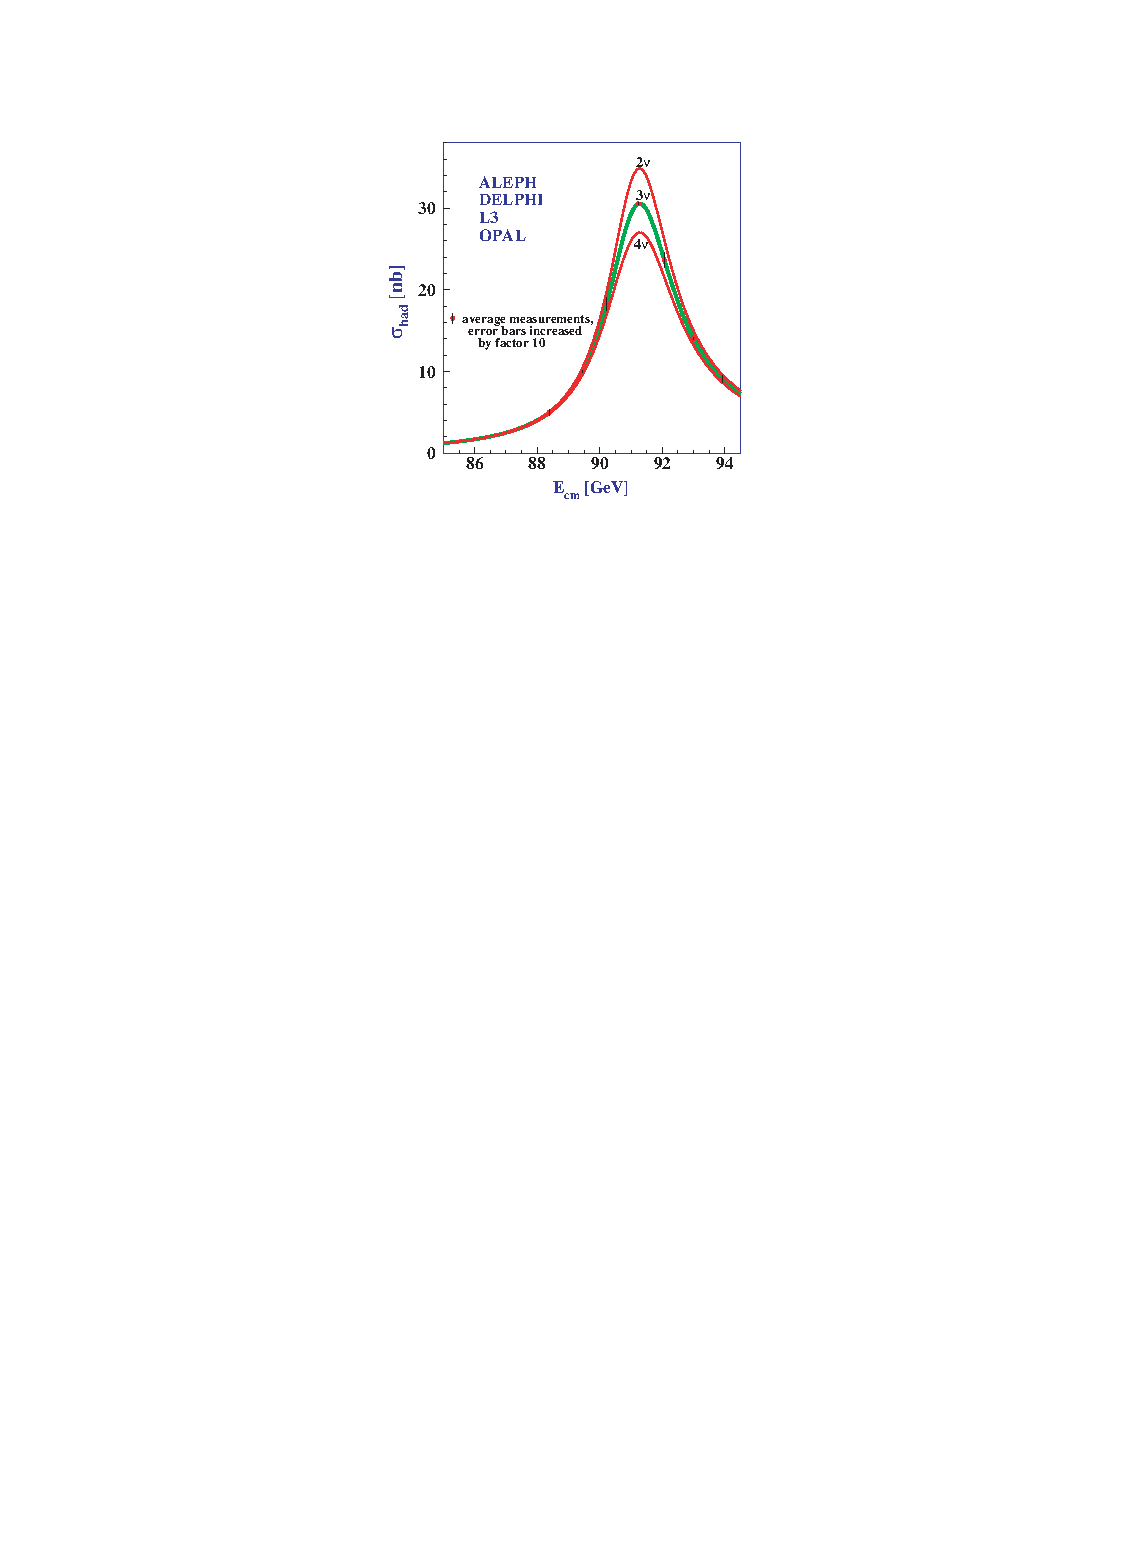
\includegraphics[width=12cm]{LEPZ0Resonance.pdf}
  \caption[Measurements of the hadron production cross-section around the Z resonance.]{Measurements of the hadron production cross-section around the Z resonance.  The curves indicate the predicted cross-section for two, three and four neutrino species with SM couplings and negligible mass.  Taken from \cite{Schael2006}.}
  \label{fig:LEPZ0Resonance}
\end{figure}

The extremely precise measurement reported by the LEP experiments was enough for many physicists to claim indisputable evidence for the existence of the tau neutrino; it was partly for this reason that its experimental discovery was not until 25 years after the addition of the $\tau$ lepton to the Standard Model.  However, in 2000 the DONUT (Direct Observation of NuTau) experiment at Fermilab, IL, U.S.A. finally reported direct detection of the tau neutrino \cite{Kodama2001}.  As its name suggests, DONUT was designed specifically for the purpose of finding the third neutrino.  It did this by identifying the $\tau$ as the only lepton at the interaction vertex from a $\nu_{\tau}$ beam created by firing 800 GeV protons from the Tevatron at a tungsten beam dump.  The mean energy of the $\nu_{\tau}$s detected at the emulsion target 36~m downstream was 111~GeV, produced by the decay of a $D_S$ meson to a $\tau$ lepton and a $\bar{\nu}_{\tau}$ neutrino followed by the decay of the $\tau$ to a $\nu_{\tau}$.  Four events were found, above a predicted background of $0.34\pm0.05$, consistent with the Standard Model description of the tau neutrino.

\subsection{The Solar Neutrino Problem}\label{SolarNeutrinoProblem}

It has been known since the 1930s, when Hans Bethe started developing the ideas of stellar nucleosynthesis \cite{Bethe1939}, that an abundance of electron neutrinos is created as byproducts of the nuclear processes powering the Sun.  The Standard Solar Model (SSM), established by John Bahcall in 1968 \cite{Bahcall1968}, explains the nuclear fusion processes responsible for powering stars.  For stars the size of the Sun, this is dominated by the \textit{proton-proton chain}; heavier stars follow the \textit{CNO cycle}.  Figure~\ref{fig:SolarNeutrinoCycles} shows the energy spectra of neutrinos released during reactions occurring during both chains.

\begin{figure}
\centering
  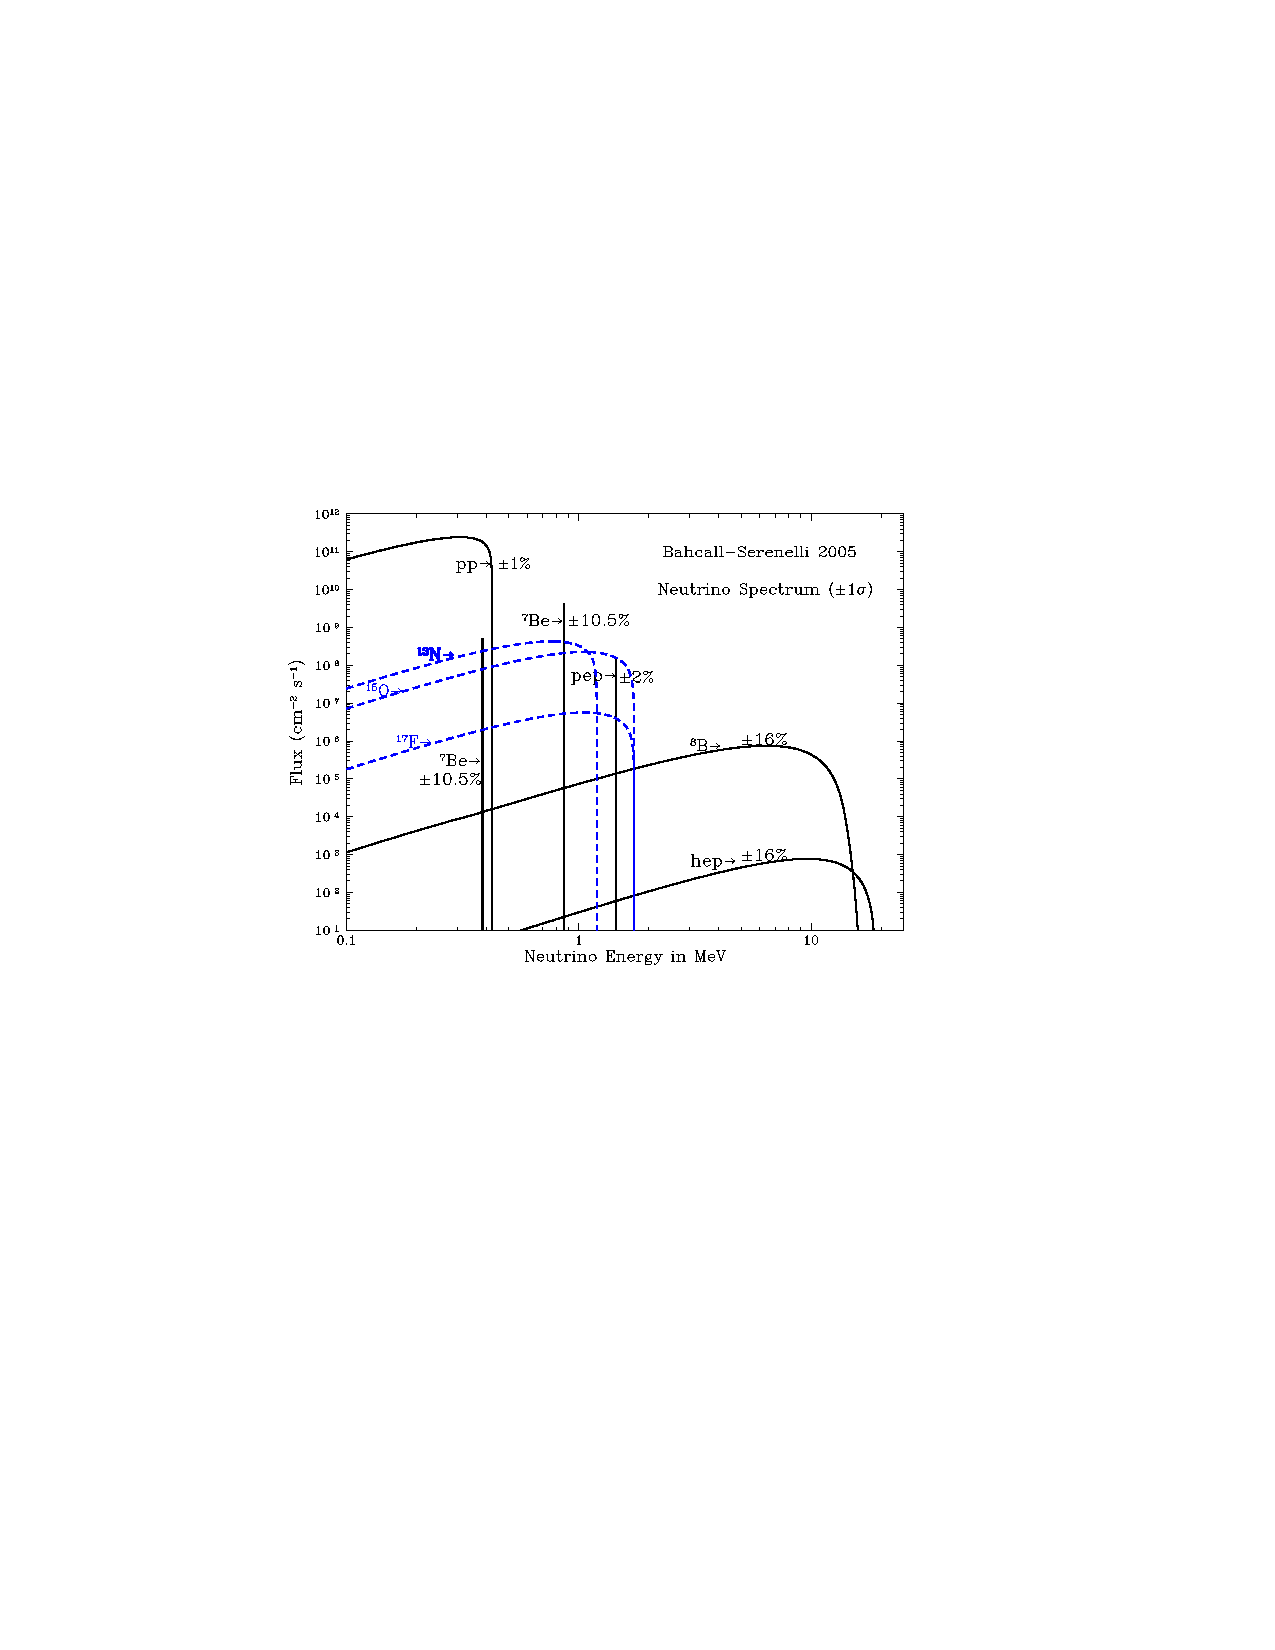
\includegraphics[width=12cm]{SolarNeutrinoCycles.pdf}
  \caption{Solar neutrino energy spectra as predicted by the Standard Solar Model \cite{Bahcall2005}.  The solid lines represent neutrinos produced during the p-p chain and dashed line represent neutrinos from the CNO cycle.  Each spectrum illustrates a particular reaction during the process of a given chain.}
  \label{fig:SolarNeutrinoCycles}
\end{figure}

Ray Davis, in collaboration with Bahcall, conducted the first experiment to detect these solar neutrinos in 1968.  Using a similar detection technique to his previous experiments, Davis used a 380~m$^3$ tank of tetrachloroethene (C$_2$Cl$_4$) to detect neutrinos via the inverse beta decay reaction detailed in Equation \ref{eq:DavisNeutrino}.  Given the threshold for this reaction is 0.814 MeV, the main sources of neutrinos probed by this experiment were Be$^7$ and B$^8$.  In order to eliminate backgrounds from cosmic rays, Davis constructed his experiment 4850~ft underground at the Homestake mine near Lead, SD, U.S.A.  It is worth noting, in a pleasing neutrino-full-circle, this is exactly where the far detector for the DUNE experiment will be housed.  The Davis Homestake experiment ran for 25 years but the results obtained \cite{Cleveland1995} disagreed quite strongly with the SSM \cite{Bahcall1995}, consistently measuring solar electron neutrinos at a rate around a third of that predicted by the model.  This became known as the `solar neutrino problem', and Davis was awarded the Nobel Prize for his work on this famous experiment in 2002.

The subsequent radiochemical experiments SAGE (from 1990) and GALLEX (from 1991) were sensitive to the large flux of \textit{pp} neutrinos by utilising a Ga$^{71}$ target and the lower threshold reaction
\begin{equation}
\nu + \textnormal{Ga}^{71} \rightarrow \textnormal{Ge}^{71} + e^-.
\end{equation}
These experiments also reported `missing' neutrinos, determining capture rates of $66.6^{+6.8+3.8}_{-7.1-4.0}$~SNU (SAGE) \cite{Abdurashitov1994} and $77.5\pm6.2^{+4.3}_{-4.7}$~SNU (GALLEX) \cite{Anselmann1992}, disagreeing with the SSM prediction of 130~SNU \cite{Hampel1999}.  There appeared to be a problem -- either the SSM was incomplete and incorrectly over-predicted the amount of electron neutrinos or hints of new physics were beginning to appear in the experiment data.

\subsection{The Atmospheric Neutrino Anomaly}\label{sec:AtmosphericNeutrinoAnomaly}

Another abundant source of natural neutrinos come from cosmic rays interacting with the upper atmosphere and producing `atmospheric neutrinos', typically via the interactions \cite{Gaisser1990}
\begin{align}
  \pi^+ \rightarrow \mu^+ + \nu_{\mu}, &\hspace{1.5cm} \mu^- \rightarrow e^- + \bar{\nu}_e + \nu_{\mu} \\
  \pi^- \rightarrow \mu^- + \bar{\nu}_{\mu}, &\hspace{1.5cm} \mu^+ \rightarrow e^+ + \nu_e + \bar{\nu}_{\mu}.
\end{align}
Since the decay lengths and kinematics are well known, the predicted ratio of muon to electron neutrinos can be calculated to a good accuracy.  This ratio can be compared to an experimentally determined ratio and analysed as a measure of the efficacy of the model.

It was first noticed as early as the late 1970s by experiments designed to search for nucleon decay predicted by the then-popular Grand Unified Theories that the measured flux did not correspond to that predicted by the theory.  The IMB \cite{Haines1986} and Kamioka \cite{Hirata1988} experiments, whilst measuring the atmospheric neutrino flux as an important background for nucleon decay, both noticed deficiencies in the ratio between muon and electron neutrinos compared to that predicted by the models.  These experiments utilised large tanks of pure water surrounded by Photo-Multiplier Tubes (PMTs) to detect neutrinos via the Cherenkov radiation created by their charged leptonic daughter particles.  Using ring-imaging techniques, it is possible to distinguish between electron-like and muon-like events and therefore identify the flavour of the incoming neutrino.  The problem implied by these measurements is known as the `atmospheric neutrino anomaly'.

Various other experiments over the following twenty years also reported similar measurements, suggesting an excess of electron neutrinos over prediction, a deficit in the number of muon neutrinos, or both.  Results from numerous experiments are shown in Figure~\ref{fig:AtmosphericNeutrinoAnomaly}.  Most experiments report a discrepancy, with its size seemingly dependent on the energy region being studied.  The experiments reporting a ratio consistent with one were much smaller than the others, and with more statistics they also started observing similar effects.  This anomaly, along with the issue of the solar neutrino problem, strongly hinted at a problem with our understanding of neutrino physics.  This is be discussed in detail in the Section \ref{sec:NeutrinoOscillations}.

\begin{figure}
  \centering
  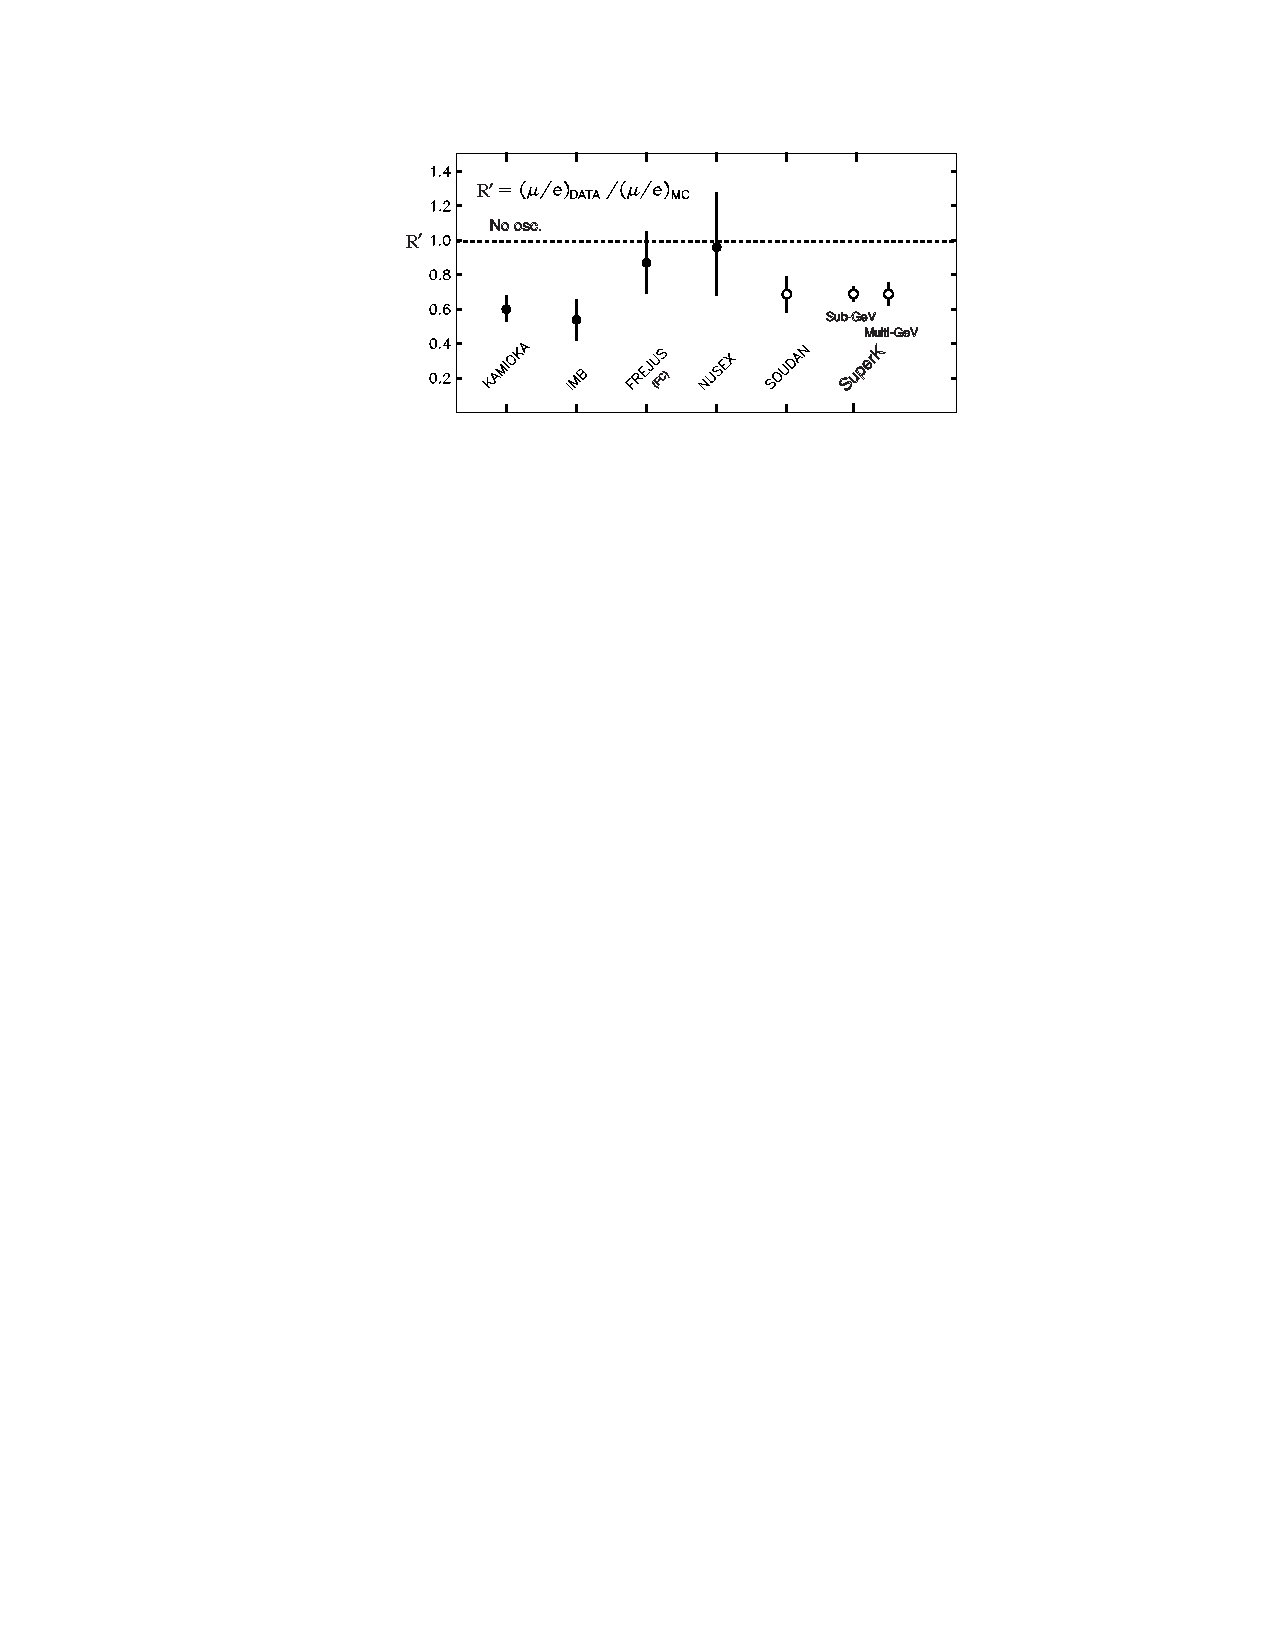
\includegraphics[width=12cm]{AtmosphericNeutrinoAnomaly.pdf}
  \caption{The double ratio \textit{R} of muon to electron neutrino events showing data divided by expectation \cite{Mann1999}.  Various underground atmospheric neutrino detectors are shown.}
  \label{fig:AtmosphericNeutrinoAnomaly}
\end{figure}

%----------------------------------------------------------------------------------------------------------------------------------------------------------------------------
\section{Neutrino Oscillations}\label{sec:NeutrinoOscillations}

The concept of neutrino oscillations involves the changing of the flavour of a neutrino as it propagates through time and space; a neutrino created in a certain flavour has a non-zero probability of being later detected in a different flavour state.  It was first postulated as an explanation of the Solar Neutrino Problem by Pontecorvo in 1968 \cite{Pontecorvo1968,Pontecorvo1969}, having initially proposed the phenomenon in 1957 as an analogy to $\textnormal{K}^0 \rightarrow \widetilde{\textnormal{K}}^0$ transition in the quark sector \cite{Pontecorvo1957}.  It offers an elegant solution to both the solar neutrino problem and the atmospheric neutrino anomaly by explaining where the `missing' neutrinos had gone; it is possible they had simply `oscillated' to a different flavour and therefore would not be detected as expected.

\subsection{The Evidence for Neutrino Oscillations}\label{sec:EvidenceNeutrinoOscillations}

Whilst there was speculation that neutrino oscillations may be the explanation behind the issues observed in the data much sooner \cite{Casper1991,BeckerSzendy1992}, definite proof was not provided until the late 1990s.  In many ways, the story of neutrino physics, from the initial observations of the Solar Neutrino Problem and the Atmospheric Neutrino Anomaly, through the speculation and theoretical developments, to the eventual proof, can be considered a triumph for the scientific method.

The Kamiokande and Super-Kamiokande experiments in Japan (upgrades from the Kamioka experiment noted previously) and the SNO experiment in Sudbury, Canada produced the results which showed indisputable evidence for neutrino oscillations and provided explanations for all previous discrepancies observed.  This result was monumental and the work of both collaborations was rewarded in 2015 when the Nobel Prize was awarded to T. Kajita and A. McDonald, from Super-Kamiokande and SNO respectively.

\subsubsection{Super-Kamiokande and the Atmospheric Sector}\label{sec:SuperKamiokande}

In 1994, the Kamiokande experiment produced results which hinted at an angular dependence for the $R$-ratio deficit, implying a dependence on neutrino travel distance \cite{Kamiokande1994}.  This result can be explained by invoking neutrino oscillations since the probability of oscillation is influenced by the propagation distance; its significantly larger successor, Super-Kamiokande, was constructed in order to make precise measurements of this phenomenon.  Super-Kamiokande is located 1000~m underground and contains an inner detector consisting of 22.5~kton fiducial volume of pure water contained within a large stainless steel cylinder (37~m high, 34~m diameter) and surrounded by 13142 20-inch photo-multipliers.  With 40\% coverage, the photocathodes extended over nearly an acre and provided ten times more pixels than any other experiment at the time.  Its results in 1998 confirmed the earlier angular dependence findings of Kamiokande, Figure~\ref{fig:SuperKamiokandeDirection}, and also considered the data as a function of neutrino energy and propagation distance, as shown in Figure~\ref{fig:SuperKamiokandeLE}.  The observed effects disagreed with a view of non-oscillating atmospheric neutrinos but were entirely consistent with a two-flavour oscillation model, $\nu_{\mu} \rightarrow \nu_{\tau}$.  This resulted in the famous published claim for the experimental discovery of neutrino oscillations \cite{SuperKamiokande1998}.

\begin{figure}
  \centering
  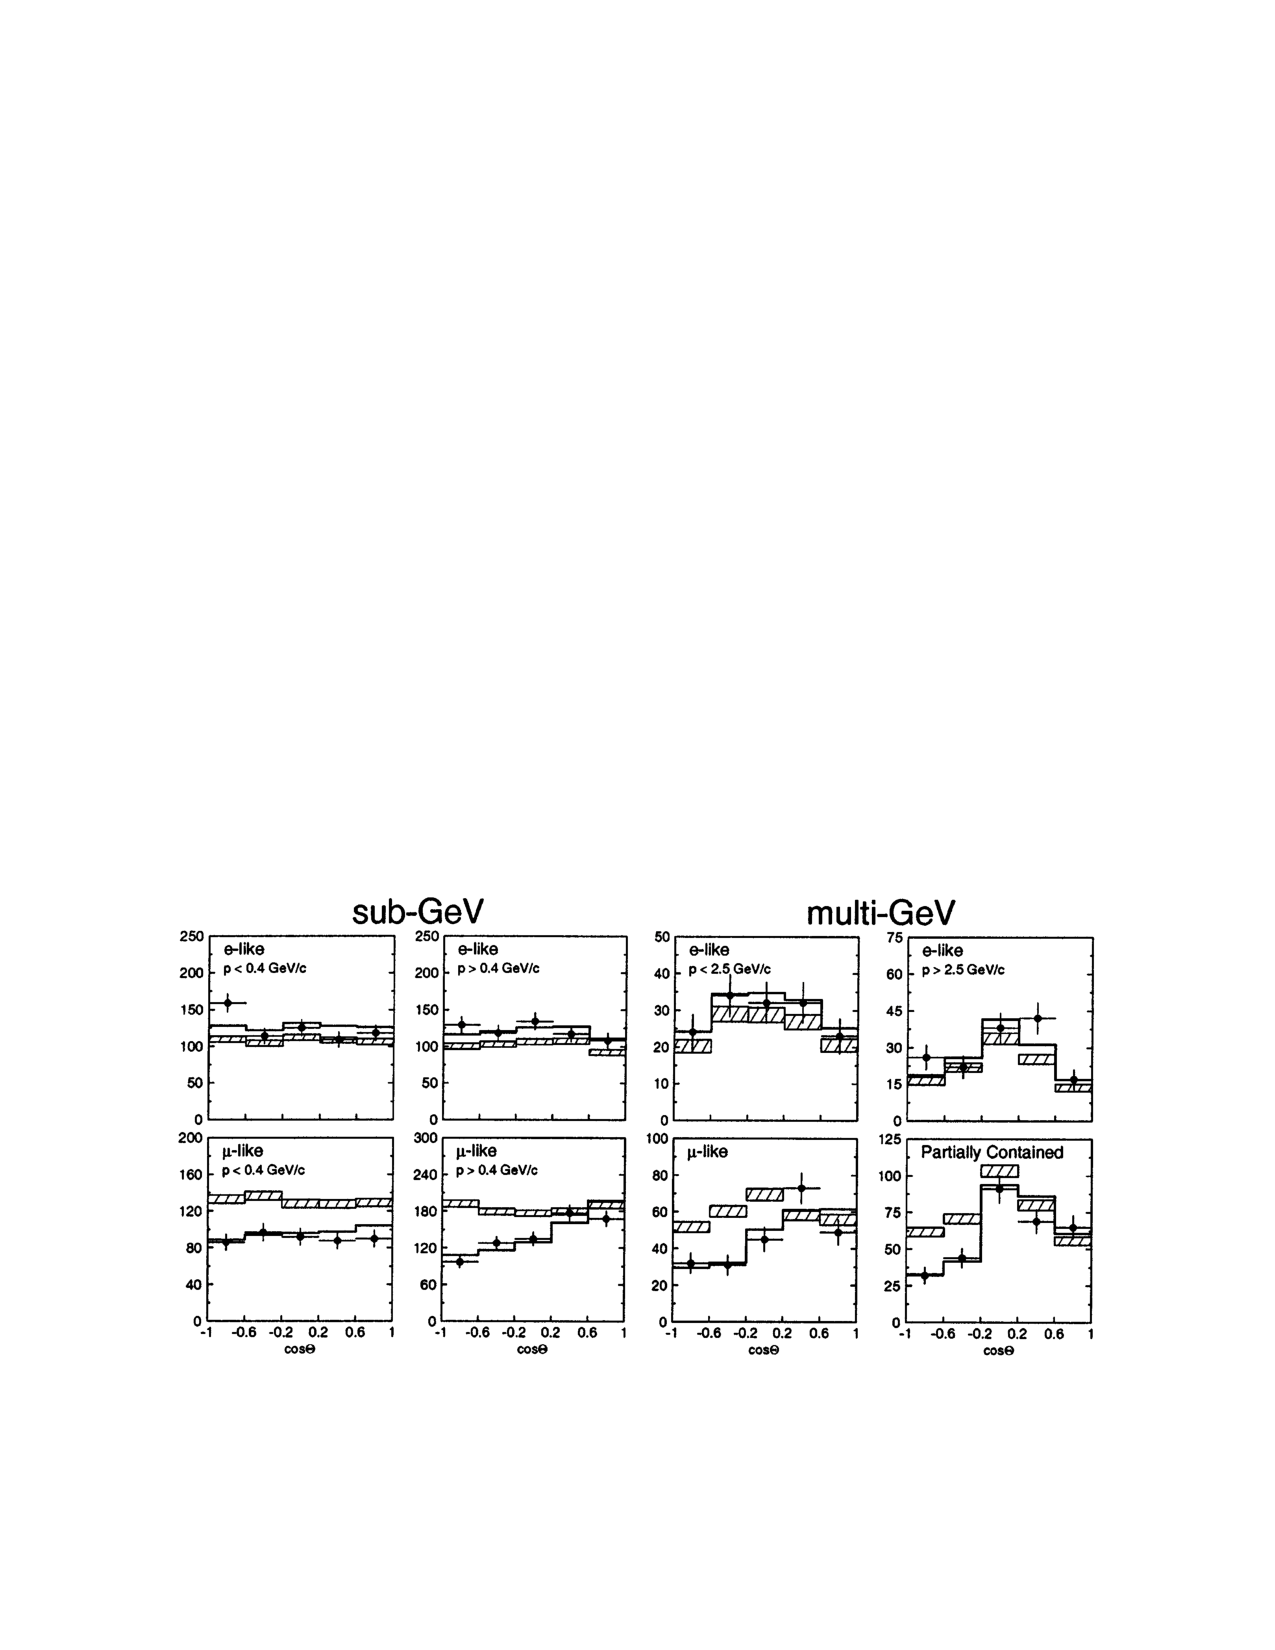
\includegraphics{SuperKamiokandeDirection.pdf}
  \caption{Zenith angle distributions of $\mu$-like and $e$-like events for sub-GeV and multi-GeV data sets.  Upward-going particles have $\cos{\Theta} < 0$ and downward-going particles have $\cos{\Theta} > 0$.  The hatched region shows the Monte Carlo expectation for no oscillations and the bold line is the best-fit expectation for $\nu_{\mu}\rightarrow\nu_{\tau}$ oscillations.  Taken from \cite{SuperKamiokande1998}.}
  \label{fig:SuperKamiokandeDirection}
\end{figure}

\begin{figure}
  \centering
  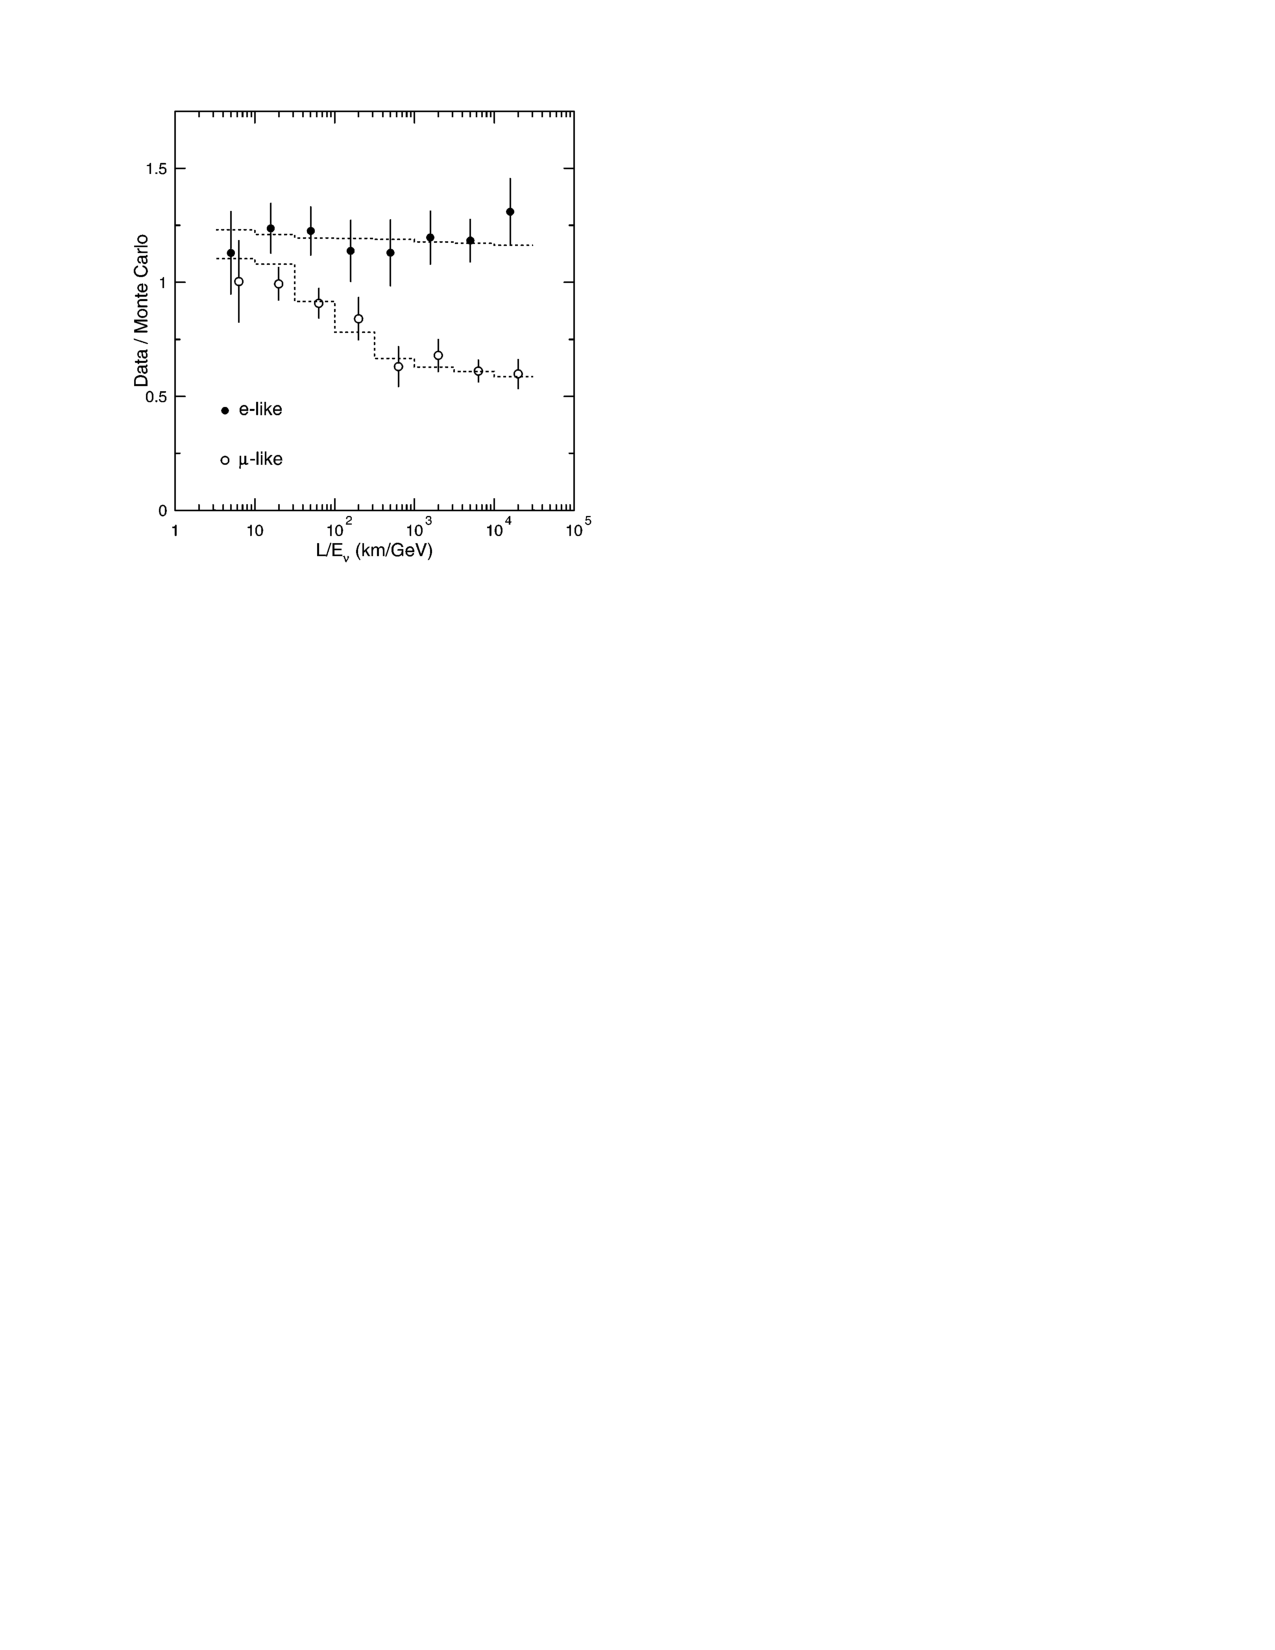
\includegraphics{SuperKamiokandeLE.pdf}
  \caption{The ratio of the number of data events to Monte Carlo events in the absence of oscillations as a function of reconstructed $L/E_{\nu}$.  The dashed lines show the expected shape for $\nu_{\mu}\rightarrow\nu_{\tau}$ oscillations.  Taken from \cite{SuperKamiokande1998}.}
  \label{fig:SuperKamiokandeLE}
\end{figure}

\subsubsection{SNO and the Solar Sector}\label{sec:SNO}

After the Super-Kamiokande results, it was clear that neutrino oscillations would probably also explain the deficit of electron neutrinos observed by solar neutrino experiments.  It took a few years until the Sudbury Neutrino Observatory (SNO) in Canada provided some quite brilliant evidence of this in 2002 \cite{SNO2002}.

SNO was a water Cherenkov detector, like Super-Kamiokande, but used heavy water (D$_2$O) as a detector medium.  The water is contained in a 12~m acrylic spherical shell and surrounded by 9456 photomultipliers at a depth of 6010~m water equivalent.  The use of heavy water facilitated sensitivity to other neutrino interaction channels not accessible by Super-Kamiokande via the charge current (CC), neutral current (NC) and elastic scattering (ES) interactions;
\begin{align}
  \nu_e + d &\rightarrow p + p + e^- &\textnormal{(CC)} \\
  \nu_x + d &\rightarrow p + n + \nu_x &\textnormal{(NC)} \\
  \nu_x + e^- &\rightarrow \nu_x + e^- &\textnormal{(ES)}.
\end{align}
The CC channel is sensitive exclusively to electron neutrinos, whilst the other two are accessible by neutrinos of any flavour.  This allowed for the first time a simultaneous measurement of the total neutrino interaction rate as well as the electron neutrino interaction rate.  The observations of SNO were the smoking gun for neutrino oscillations; the total measured flux for all neutrinos, $\phi_{\textnormal{NC}}^{\textnormal{SNO}} = 6.42\pm1.57\textnormal{~(stat.)}^{+0.55}_{-0.58}\textnormal{~(sys.)}$~cm$^{-2}$s$^{-1}$, agreed excellently with the electron neutrino flux predicted by the SSM, $\phi^{\textnormal{SSM}} = 5.05^{+1.01}_{-0.81}$~cm$^{-2}$s$^{-1}$.  However, the measured electron neutrino flux was around a third lower, $\phi_e^{\textnormal{SNO}} = 1.76\pm0.05\textnormal{~(stat.)}\pm0.09\textnormal{~(sys.)}$~cm$^{-2}$s$^{-1}$, consistent with previous measurements from the radiochemical experiments.  The evidence seems conclusive: the solar models are correct and the neutrinos are not disappearing; there are simply changing their flavour state.  A summary plot showing all solar neutrino experiments up until this point is depicted in Figure~\ref{fig:SolarNeutrinoFluxes} \cite{Bahcall2005Fluxes}.

\begin{figure}
  \centering
  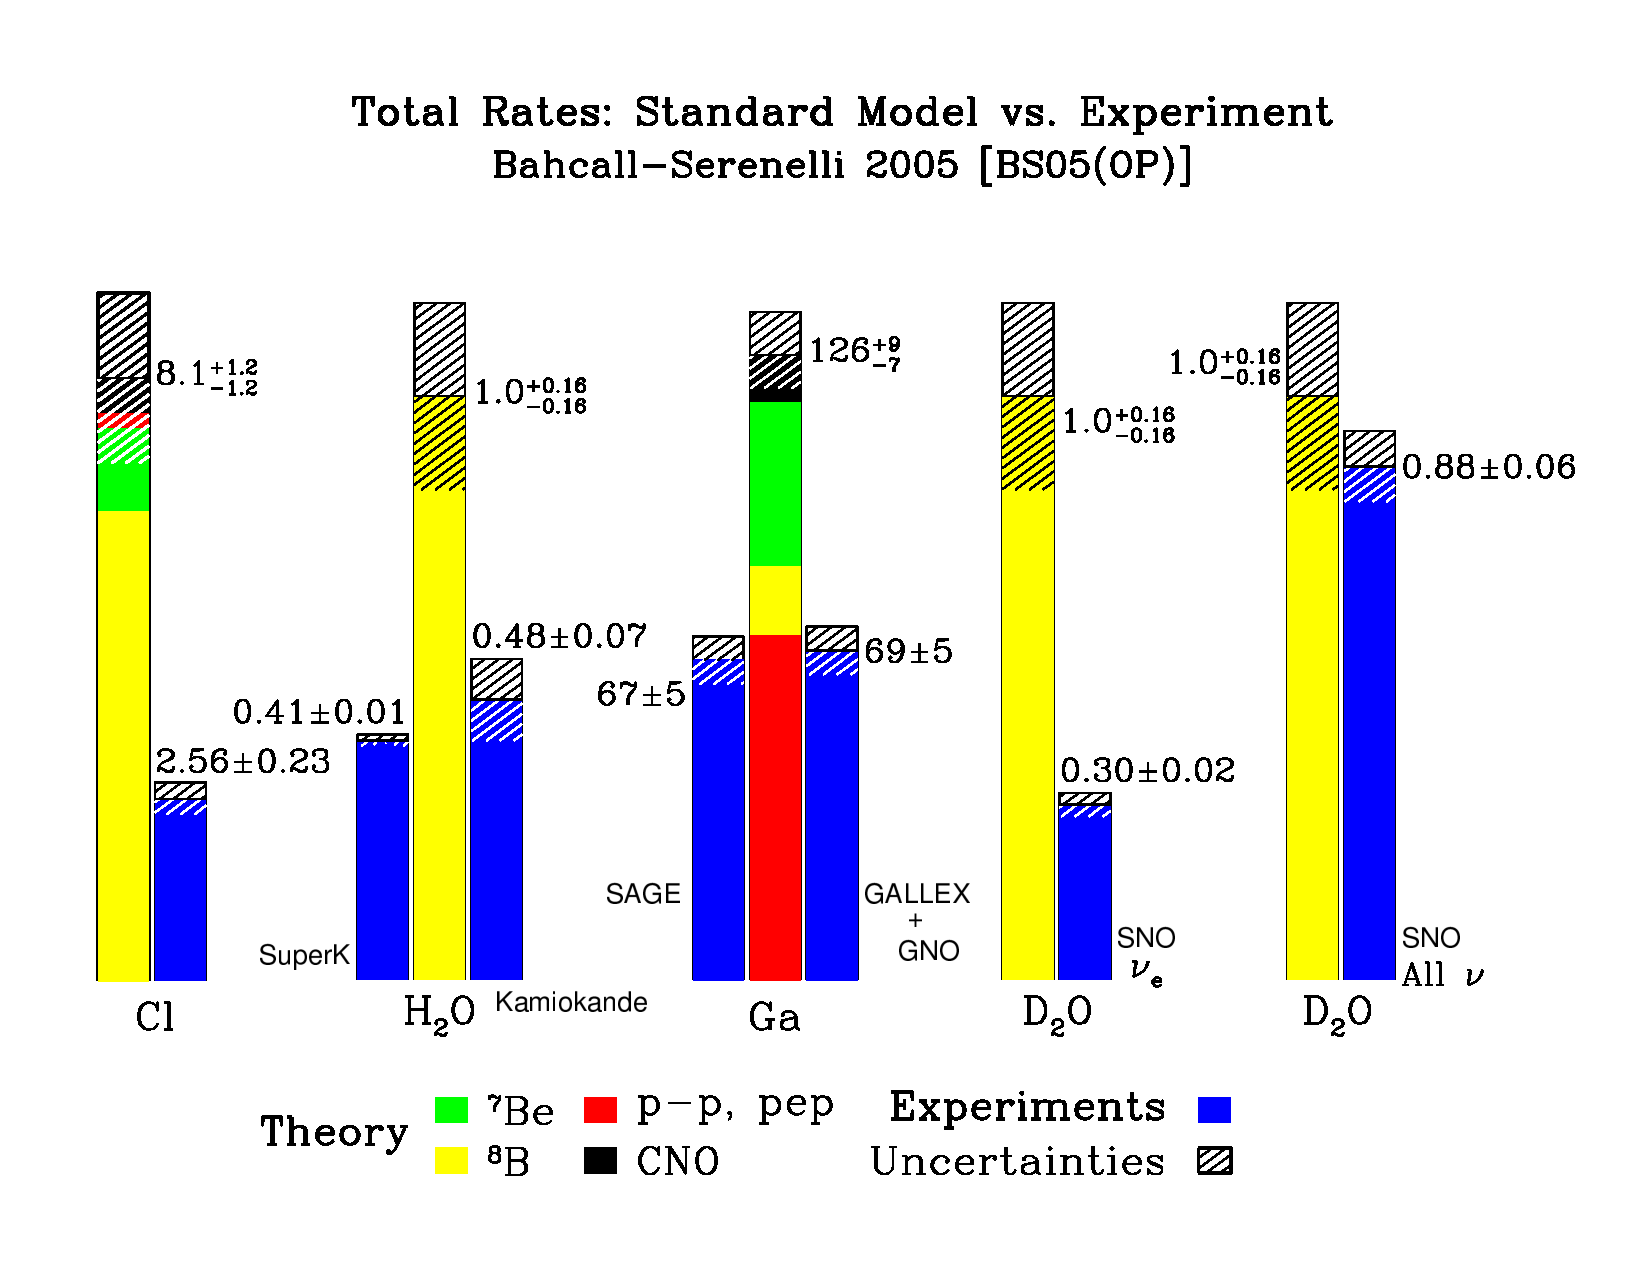
\includegraphics[width=16cm]{SolarNeutrinoFluxes.pdf}
  \caption{Comparison of the predictions of the neutrino fluxes from the Standard Solar Model with measured rates from a variety of solar neutrino experiments.  The results of SNO (D$_2$O target, right two comparisons) show that the expected flux is observed, but not necessarily as electron neutrinos.  This shows conclusively the oscillatory nature of neutrinos.}
  \label{fig:SolarNeutrinoFluxes}
\end{figure}

\subsection{Vacuum Oscillations}\label{sec:VacuumOscillations}

The theory of neutrino oscillations is basically the quantum mechanics of mixed states and was developed on top of Pontecorvo's work by Ziro Maki, Masami Nakagawa and Shoichi Sakata \cite{MNS1962}.  If the neutrino flavour states can spontaneously convert from one to another, none can be considered as eigenfunctions of the Hamiltonian.  The true stationary states are the \textit{mass eigenstates} ($\nu_1$, $\nu_2$, $\nu_3$), of which the flavour states ($\nu_e$, $\nu_{\mu}$, $\nu_{\tau}$) can be considered linear superpositions:
\begin{equation}
  \begin{pmatrix}
    \nu_e \\
    \nu_{\mu} \\
    \nu_{\tau} \\
  \end{pmatrix}
  =
  U^*_{\textnormal{PMNS}}
  \begin{pmatrix}
    \nu_1 \\
    \nu_2 \\
    \nu_3 \\
  \end{pmatrix},
  \label{eq:FlavourMassStates}
\end{equation}
where $U_{\textnormal{PMNS}}$ is the PMNS mixing matrix which described the flavour composition of each of the mass eigenstates, and vice versa.  If the PMNS matrix were diagonal, each flavour state would correspond to a single mass state and oscillations would not occur.

Just as the flavour states are a superposition of mass states
\begin{equation}\label{eq:FlavourSuperposition}
  \ket{\nu_{\alpha}} = \sum_i U^*_{\alpha i} \ket{\nu_i},
\end{equation}
the mass states can also be considered a superposition of flavour states
\begin{equation}\label{eq:MassSuperposition}
  \ket{\nu_i} = \sum_{\alpha} U_{\alpha i} \ket{\nu_{\alpha}}.
\end{equation}

For the three neutrino case, the PMNS matrix, decomposed into its three axial rotations, can be expressed as
\begin{equation}
  U_{\alpha i} \equiv
  \underbrace{
    \begin{pmatrix}
      1 & 0 & 0 \\
      0 & c_{23} & s_{23} \\
      0 & -s_{23} & c_{23} \\
    \end{pmatrix}
  }_{\textnormal{`Atmospheric' term}}
  \underbrace{
    \begin{pmatrix}
      c_{13} & 0 & e^{-i\delta} s_{13} \\
      0 & 1 & 0 \\
      -e^{-i\delta} s_{13} & 0 & c_{13} \\
    \end{pmatrix}
  }_{\textnormal{`Accelerator' or `Reactor' term}}
  \underbrace{
    \begin{pmatrix}
      c_{12} & s_{12} & 0 \\
      -s_{12} & c_{12} & 0 \\
      0 & 0 & 1 \\
    \end{pmatrix}
  }_{\textnormal{`Solar' term}}
  ,
  \label{eq:PMNS}
\end{equation}
where $c_{ij} \equiv \cos{(ij)}$, $s_{ij} \equiv \sin{(ij)}$ and $\delta$ is a CP-violating phase factor.  Each axial component is often referred to by the means with which they are studied, as shown in Equation \ref{eq:PMNS}.

The weak interaction couples to the flavour eigenstates so neutrinos are always created and detected as flavour states.  However, they propagate as mass states since it is these which are eigenstates of the Hamiltonian.  Due to the misalignment of the flavour and mass states, oscillations can be shown to occur.  A neutrino created with flavour $\alpha$ is a superposition of all the mass states (Equation \ref{eq:FlavourSuperposition}).  These states propagate as a plane wave, evolving in time and space such that
\begin{equation}\label{eq:MassTimeEvolution}
  \ket{\nu_i(x,t)} = \ket{\nu_i (0)} e^{-i \textbf{x} \cdot \textbf{p}},
\end{equation}
where \textbf{x} and \textbf{p} are the 4-position and 4-momentum of the neutrino respectively.  From Equations \ref{eq:FlavourSuperposition} and \ref{eq:MassTimeEvolution}, the evolution of the flavour states over space and time is therefore
\begin{align}
  \nonumber \ket{\nu_{\alpha}(x,t)} &= \sum_i U_{\alpha i}^* \ket{\nu_i (x,t)} \\
  \label{eq:FlavourTimeEvolution} &= \sum_i U_{\alpha i}^* e^{-i \textbf{x} \cdot \textbf{p}} \ket{\nu_i(0)} .
\end{align}
In the ultra-relativistic limit, the mass of the neutrino is negligible compared to its momentum ($m_i \ll \vec{p}$) and $\vec{x} \approx ct$;
\begin{align}
  \label{eq:RelativisticEnergy} E_i &= \sqrt{|\vec{p}|^2+m_i^2} = \vec{p}\sqrt{1+\frac{m_i^2}{|\vec{p}|^2}} \approx \vec{p}+\frac{m_i^2}{2\vec{p}} \\
  \label{eq:RelativisticEnergyMomentum} \textbf{x}\cdot\textbf{p} &= E_i t - \vec{x}\cdot\vec{p} = \vec{p}\cdot t + \frac{m_i^2}{2\vec{p}}t - \vec{x}\cdot\vec{p} \approx \frac{m_i^2}{2\vec{p}}\vec{x} = \frac{m_i^2}{2p}x ,
\end{align}
assuming the neutrino displacement is in the direction of its momentum and using natural units ($c \equiv \hbar \equiv 1$).  Thus, using Equations \ref{eq:FlavourTimeEvolution}, \ref{eq:RelativisticEnergyMomentum} and \ref{eq:MassSuperposition},
\begin{align}
  \nonumber \ket{\nu_{\alpha}(x,t)} &= \sum_i U_{\alpha i}^* e^{-i \frac{m_i^2}{2p} x} \ket{\nu_i (0)} \\
  \label{eq:FlavourEvolution} &= \sum_i \sum_{\beta} U_{\alpha i}^* e^{-i \frac{m_i^2}{2p} x} U_{\beta i} \ket{\nu_{\beta}}.
\end{align}

The probability of a neutrino created in flavour state $\alpha$ being observed in flavour $\beta$ can be determined from Equation \ref{eq:FlavourEvolution}
\begin{align}
  P(\alpha \rightarrow \beta) &= |\braket{\nu_{\alpha}}{\nu_{\beta}(x,t)}|^2 \\
  &= \left[ \sum_i U_{\alpha i} e^{i \frac{m_i^2}{2p} x} U_{\beta i}^* \right] \left[ \sum_j U_{\alpha j}^* e^{-i \frac{m_j^2}{2p} x} U_{\beta j} \right] \\
  &= \sum_{i,j} U_{\alpha i} U_{\alpha j}^* U_{\beta j} U_{\beta i}^* e^{i \frac{m_i^2-m_j^2}{2p} x},
\end{align}
and is observed to be dependent on the neutrino momentum, the difference between the squared masses of the flavour states, the propagation distance and the relative mixing of the two flavour states encoded in the matrix elements $U$.

An accelerator based neutrino experiment, such as DUNE, will typically use a $\nu_{\mu}$-dominated beam and look for \textit{muon neutrino disappearance} ($P(\nu_{\mu}\rightarrow \nu_{\mu})$) and \textit{electron neutrino appearance} ($P(\nu_{\mu}\rightarrow \nu_e)$).  In this case, also in the relativistic limit, the relevant appearance and disappearance probabilities can be approximated, respectively, as
\begin{align}
  \label{eq:ElectronNeutrinoAppearance} P(\nu_{\mu} \rightarrow \nu_e) &\approx \sin^2{2\theta_{13}} \sin^2{\theta_{23}} \sin^2 {\left( 1.27 \frac{\Delta m_{13}^2 L}{E} \right)} \\
  \label{eq:MuonNeutrinoDisappearance} P(\nu_{\mu} \rightarrow \nu_{\mu}) &\approx 1 - \cos^4{\theta_{13}} \sin^2{2\theta_{23}} \sin^2{ \left( 1.27 \frac{\Delta m_{23}^2 L}{E} \right) },
\end{align}
where $\Delta m_{ij}^2 \equiv m_i^2-m_j^2$ is the \textit{mass squared splitting} in eV, $L$ is the distance propagated in km and $E$ is the neutrino energy in GeV.

From these equations, it can be seen the important controllable parameters relevant for observing oscillations are the neutrino energy and the distance they travel.  An experiment will typically choose a ratio $L/E$ which will attempt to maximise the effect of oscillations in order to make precision measurements.

\subsection{Matter Effects}\label{sec:MatterEffects}

The oscillations considered thus far are \textit{vacuum oscillations} which occur due to the mixing of the neutrino mass and flavour states.  Whilst directly confirming the oscillation of solar neutrinos, the SNO experiment (along with every other solar neutrino experiment) reported more oscillations than can be explained using just the vacuum oscillation model discussed in Section \ref{sec:VacuumOscillations} \cite{Bahcall2002,Smirnov2003}.  When neutrinos propagate through matter, an additional potential can be shown to also produce oscillations, which would occur even in the case of massless neutrinos (as long as mixing occurs).  Since solar neutrinos travel through dense matter before exiting the Sun, it is possible these matter effects explained above could explain this discrepancy.

Coherent scattering (scattering in which the neutrino state is unchanged) due to interactions with the medium cause neutrinos travelling through matter to feel a potential.  As normal matter is composed of electrons, rather than their heavier counterparts muons and taus, electron neutrinos are affected more by this potential.  The mechanism for this is demonstrated in Figure~\ref{fig:MatterEffects}.  This gives rise to an additional effective mass splitting between the electron neutrino and the other flavours and therefore results in the possibility of oscillations \cite{Wolfenstein1978}.  Due to the density of the Sun and the neutrino energies, the neutrinos actually feel a resonance which causes their oscillation probability to become dramatically higher than the vacuum oscillation probabilities.  This is known as the Mikheev-Smirnov-Wolfenstein (MSW) effect \cite{MS1985,MS1986}.  It is worth pointing out at this point that, since normal matter is composed of electrons and not positrons, this effect is also different for $\nu_e$s and $\bar{\nu}_e$s; the importance of this becomes apparent when considering the additional effects of CP-violation.

\begin{figure}
  \centering
  \begin{subfigure}{0.48\linewidth}
    \centering
    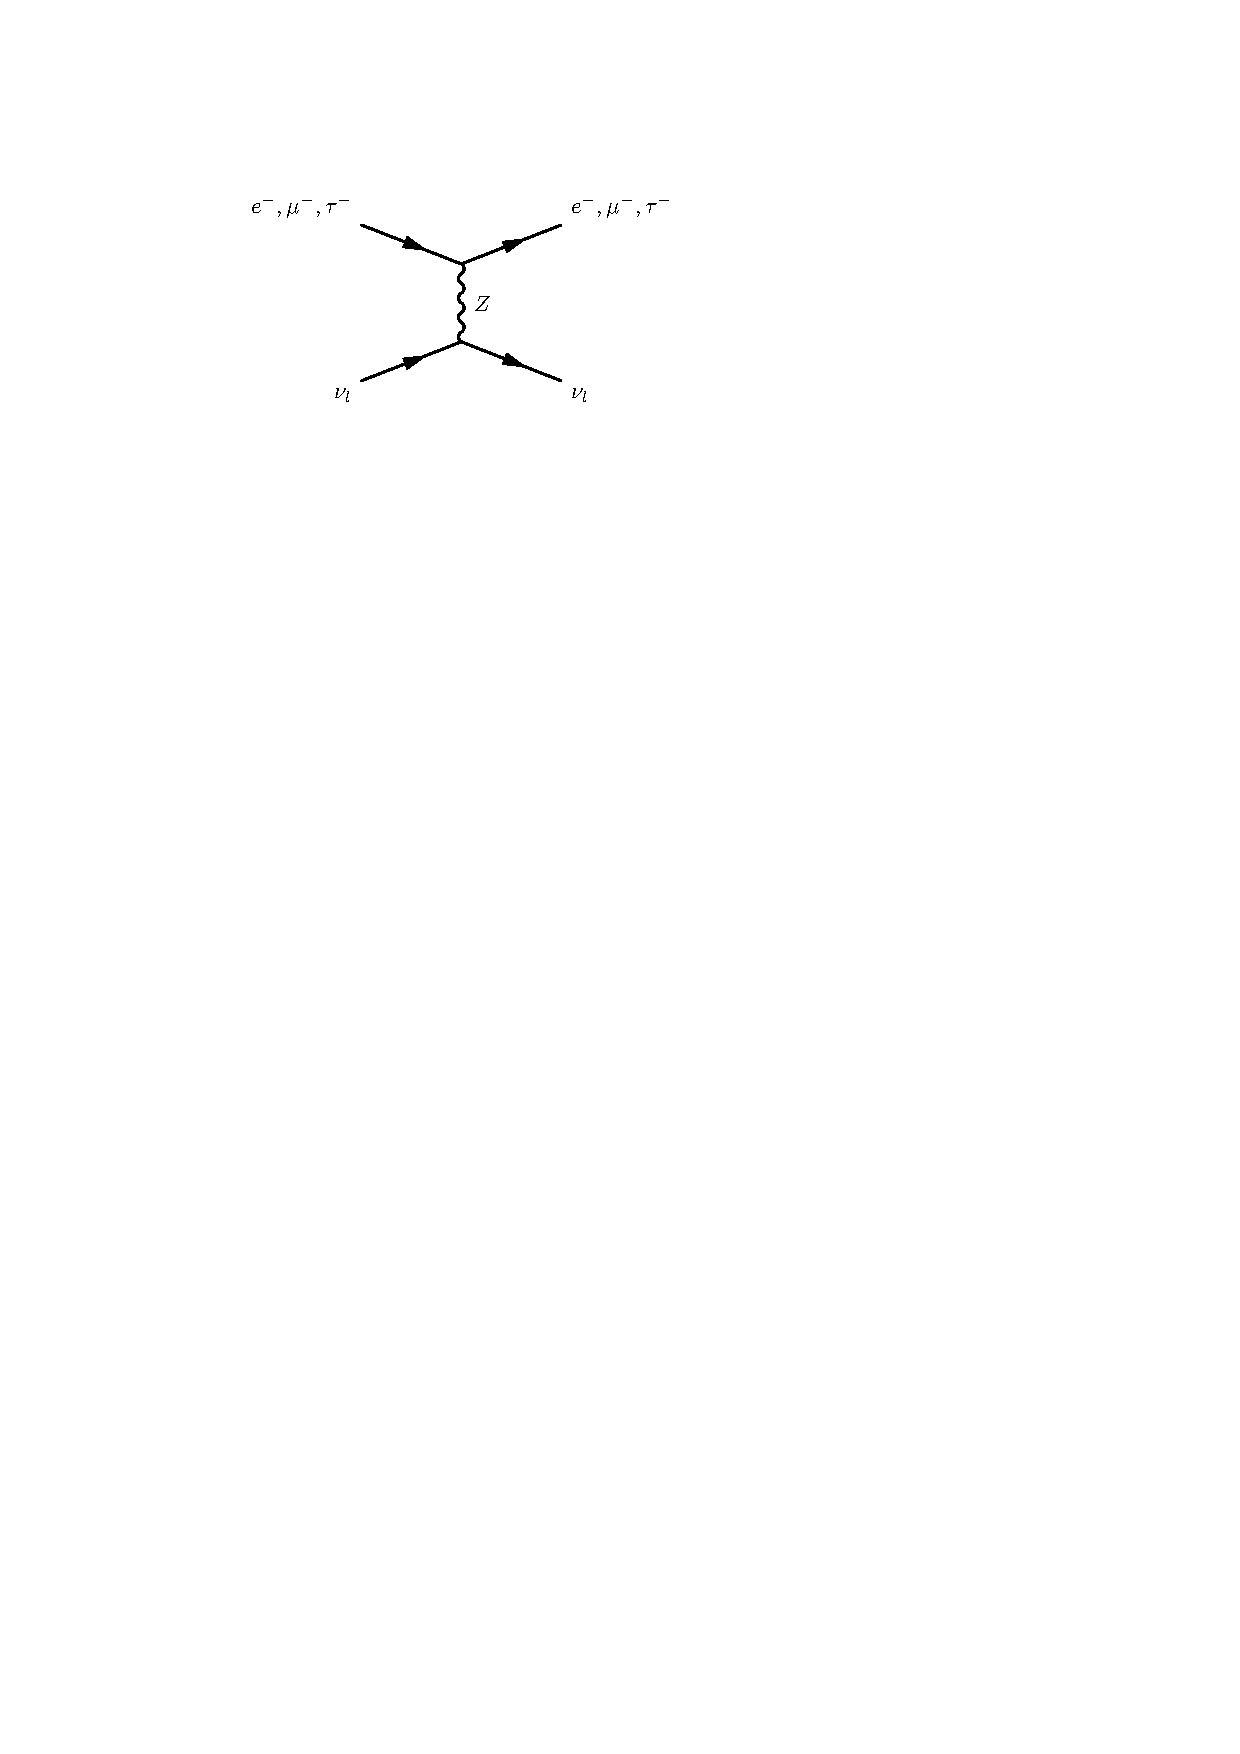
\includegraphics{MatterEffectsNC.pdf}
    \caption{Neutral current scattering.}
    \label{fig:MatterEffectsNC}
  \end{subfigure}
  \hfill
  \begin{subfigure}{0.48\linewidth}
    \centering
    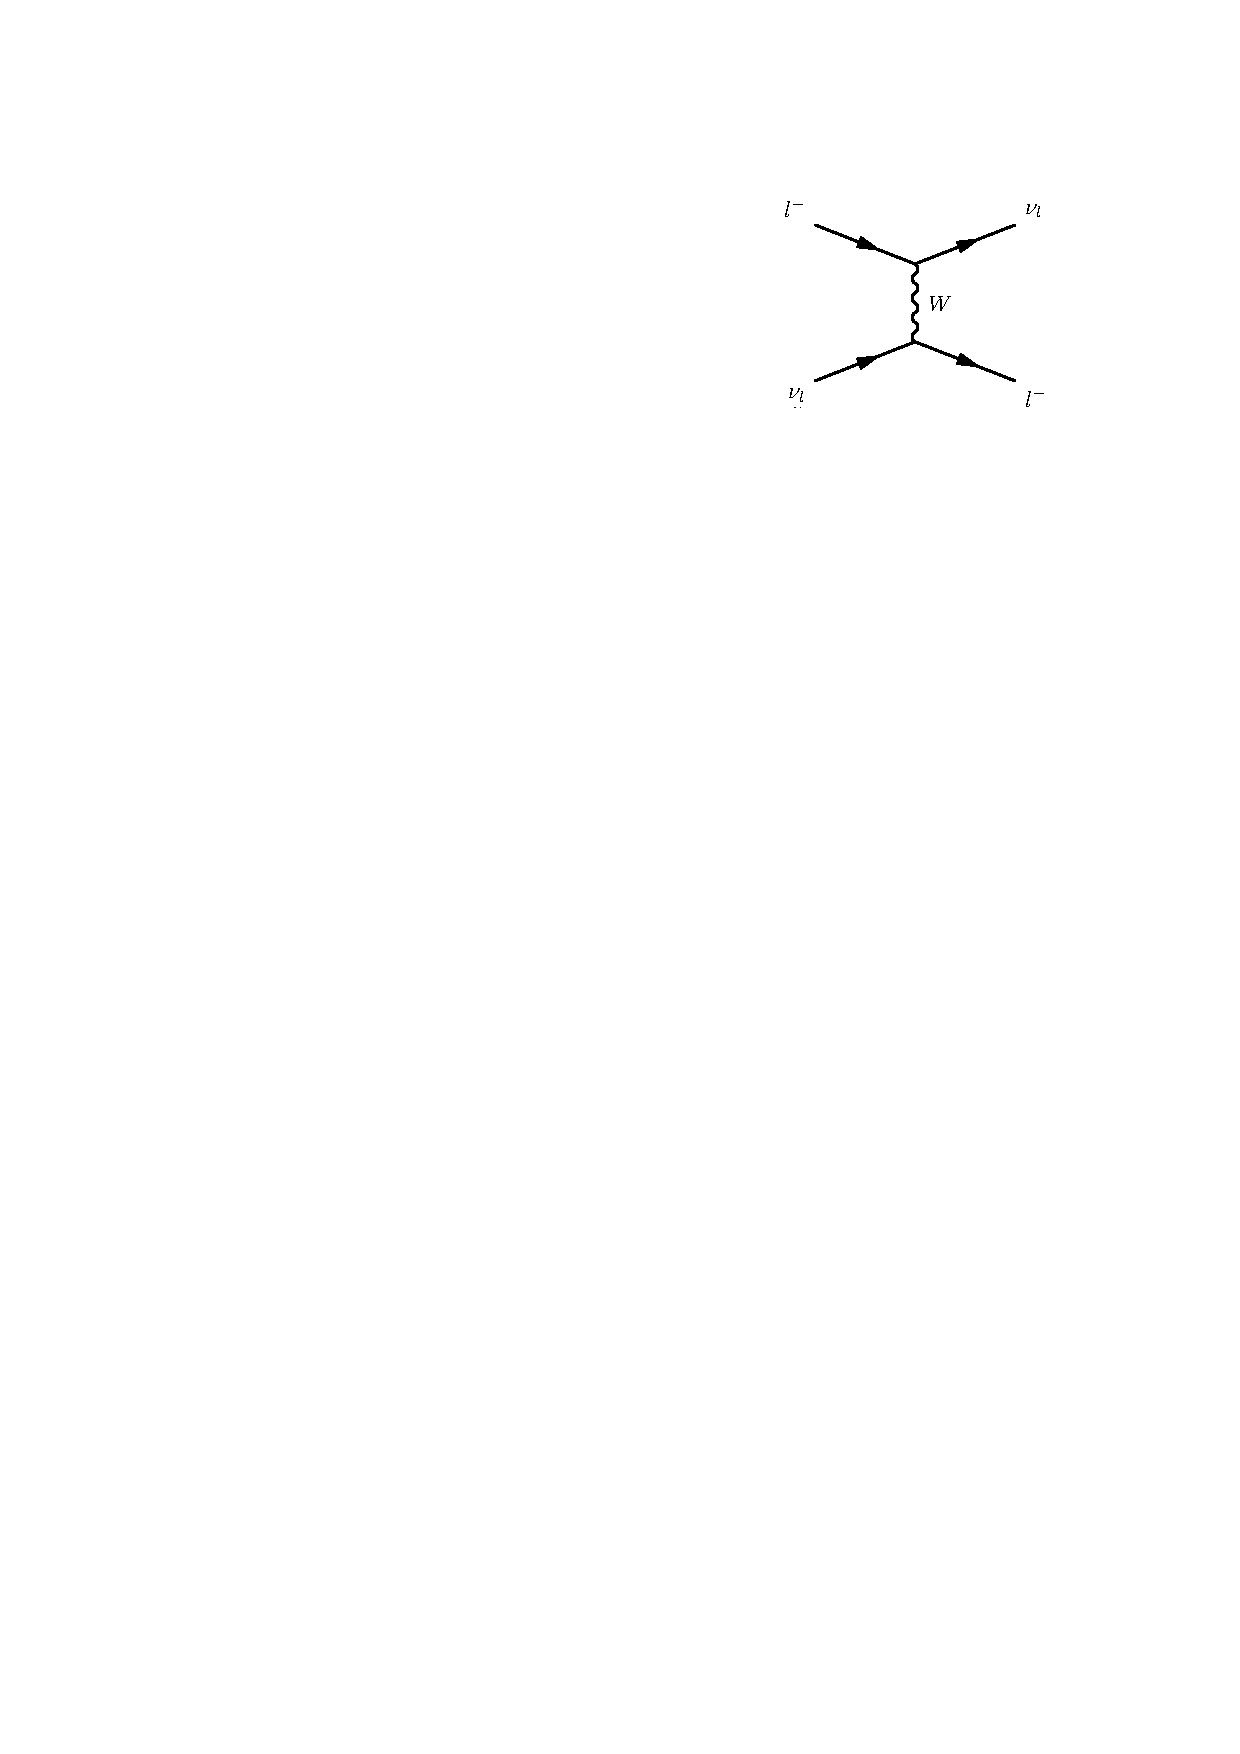
\includegraphics{MatterEffectsCC.pdf}
    \caption{Charged current scattering.}
    \label{fig:MatterEffectsCC}
  \end{subfigure}
  \caption{General scattering mechanics which occur as neutrinos pass through matter.  Neutral current scattering (Figure~\ref{fig:MatterEffectsNC}) occurs for all neutrino flavour combinations whereas charged current scattering (Figure~\ref{fig:MatterEffectsCC}) only occurs when the incoming leptons have the same flavour.}
  \label{fig:MatterEffects}
\end{figure}

\subsubsection{KamLAND and Reactor Neutrinos}\label{sec:KamLAND}

In order to investigate the possible MSW effects in the Sun, measurements of electron neutrino disappearance from terrestrial neutrinos, which were not subject to these matter effects, were considered.  The first experiment to publish results was KamLAND (Kamioka Liquid Scintillator Anti-Neutrino Detector) in 2003 \cite{KamLAND2003,KamLAND2005}.  KamLAND occupied the site previously used by the Kamiokande experiment in Japan under 2700 m.w.e of rock and utilised 1~kton of ultra-pure liquid scintillator contained in a 13~m spherical balloon.  It was surrounded by 53 Japanese nuclear power reactors with baselines ranging from ~80~km to 800~km and detected the $\bar{\nu}_e$s via the inverse beta decay reaction $\bar{\nu}_e + p \rightarrow e^+ + n$.  Scintillation light from the delayed coincidence of a positron with the neutron capture was detected using 1879 PMTs and constituted a signal with very low background.  The results from KamLAND confirmed the apparently large matter effect in solar neutrinos and completely solved for the first time the long-standing Solar Neutrino Problem \cite{Bandyopadhyay2002,deHolanda2002,Fogli2003}.

\subsection{CP-Violation}\label{sec:CPViolation}

The $\delta$ terms in Equation \ref{eq:PMNS} are CP-violating phase factors.  They could be included in any of the diagonalised components but are generally added to the accelerator part since this is how current and future experiments will look for evidence of CP-violation.  As long as all the mixing angles are non-zero, there is the possibility of CP-violation in the lepton sector.

This is an exciting prospect and one of the reasons for the current intense interest in neutrino physics.  It is known CP-violating processes must have occurred in the early Universe since matter has come to dominate massively over antimatter after they were created equally in the Big Bang.  This has been observed in the quark sector but current experimental evidence can only account for a small amount of the necessary CP-violation.  It is also expected but has never been observed in strong interactions \cite{Mannel2007}.  Leptonic CP-violation could potentially account for the matter-antimatter asymmetry in the Universe and ultimately explain how it evolved to include our very existence \cite{Ohlsson2012,Ohlsson2013}.

In neutrino experiments, effects of CP-violation would be apparent as a difference in behaviour between neutrinos and antineutrinos.  For example, since the sign of $\delta$ is different for neutrinos and antineutrinos, an asymmetry
\begin{equation}\label{eq:NeutrinoAntineutrinoAsymmetry}
  \mathcal{A} = \frac{P(\nu_{\mu}\rightarrow\nu_e)-P(\bar{\nu}_{\mu}\rightarrow\bar{\nu}_e)}{P(\nu_{\mu}\rightarrow\nu_e)+P(\bar{\nu}_{\mu}\rightarrow\bar{\nu}_e)}
\end{equation}
can be observed and measured.

%----------------------------------------------------------------------------------------------------------------------------------------------------------------------------
\section{Status of Neutrino Physics}\label{sec:NeutrinoPhysicsStatus}

The field of neutrino physics has advanced rapidly over the past twenty to thirty years (discussed in Sections \ref{sec:HistoricalContext} and \ref{sec:NeutrinoOscillations}) and there is currently a good understanding of most experimental results in the context of 3-flavour neutrino oscillations.  Presently, the focus has shifted to making precise measurements of the oscillation parameters and trying to understand the nature of neutrino mass.  The current understanding of each of these areas will be presented in Sections \ref{sec:OscillationParameters} and \ref{sec:NeutrinoMass} respectively following a brief overview of current and future experiments in Section \ref{sec:CurrentExperiments}.

%----------------------------------------------------------------------------------------------------------------------------------------------------------------------------
\subsection{Current and Future Experiments}\label{sec:CurrentExperiments}

In recent years, neutrino experiments which utilise a custom built artificial neutrino beam have been offering complimentary and world-leading results.  These `accelerator experiments' are used in order to have more control over the energy spectrum and composition of the neutrino beam and often use a long-baseline, sampling the beam at different points to determine the effects of oscillation as the neutrinos propagate in between.

MINOS was based at Fermilab, U.S., and detected neutrinos from the NuMI (Neutrinos at the Main Injector) beam at a `near detector' and then again in Northern Minnesota, a baseline of 735~km.  T2K follows a similar design and uses the Super-Kamiokande detector as the far detector, utilising a beam from J-PARC, Japan and a baseline of 295~km.  T2K and NO$\nu$A, another current long-baseline experiment, were designed specifically to measure the last mixing parameter, $\theta_{13}$, by looking for $\nu_e$ appearance in a $\nu_{\mu}$ beam.  NO$\nu$A, like its predecessor MINOS, also uses the NuMI beam and has a far detector at the same site.  However, along with T2K, it is `off-axis' by around $2^{\circ}$; this produces a more monotonic neutrino energy spectrum to maximise the effect of oscillations and make more accurate measurements.  T2K and NO$\nu$A still have many years left of their respective programmes and are currently making precision measurements of the mixing parameters along with constraining CP-violation by combining neutrino and antineutrino analyses.  They will not be able to make statistically significant measurements of this area but, especially through joint analyses, will be able to offer hints before the next generation of experiments.

Future long-baseline experiments include DUNE \cite{DUNECDR1}, which will be discussed properly in Chapter \ref{chap:DUNE}, and Hyper-Kamiokande \cite{HyperKamiokande2015}, an upgrade of the current T2K experiment.  Hyper-Kamiokande will also use water Cherenkov technology but will boast a fiducial volume 25 times larger than that of Super-Kamiokande.  The timescale of these projects is on the order of at least ten years from now and both pose incredible engineering challenges in their own right.

%----------------------------------------------------------------------------------------------------------------------------------------------------------------------------
\subsection{Oscillation Parameters}\label{sec:OscillationParameters}

The current status of the mixing angles and the mass-squared differences is depicted in Figure~\ref{fig:GlobalFit}.  The world-best measurements for $\theta_{12}$ and $\Delta m^2_{12}$ are provided by the solar neutrino experiments (Homestake \cite{Cleveland1995}, GALLEX \cite{Gallex2010}, SAGE \cite{Sage2009} and SNO \cite{SNO2013}) and KamLAND \cite{KamLAND2013}.  The leading measurements in the atmospheric neutrino sector, $\theta_{23}$ and $|\Delta m_{32}^2|$, are from Super-Kamiokande \cite{SuperKamiokande2010}, IceCube \cite{IceCube2015} and the accelerator experiments MINOS \cite{MINOS2013,MINOS2013b}, T2K \cite{T2Knumu2014} and NO$\nu$A \cite{NOvAnumu2016}.

\begin{figure}[p]
  \centering
  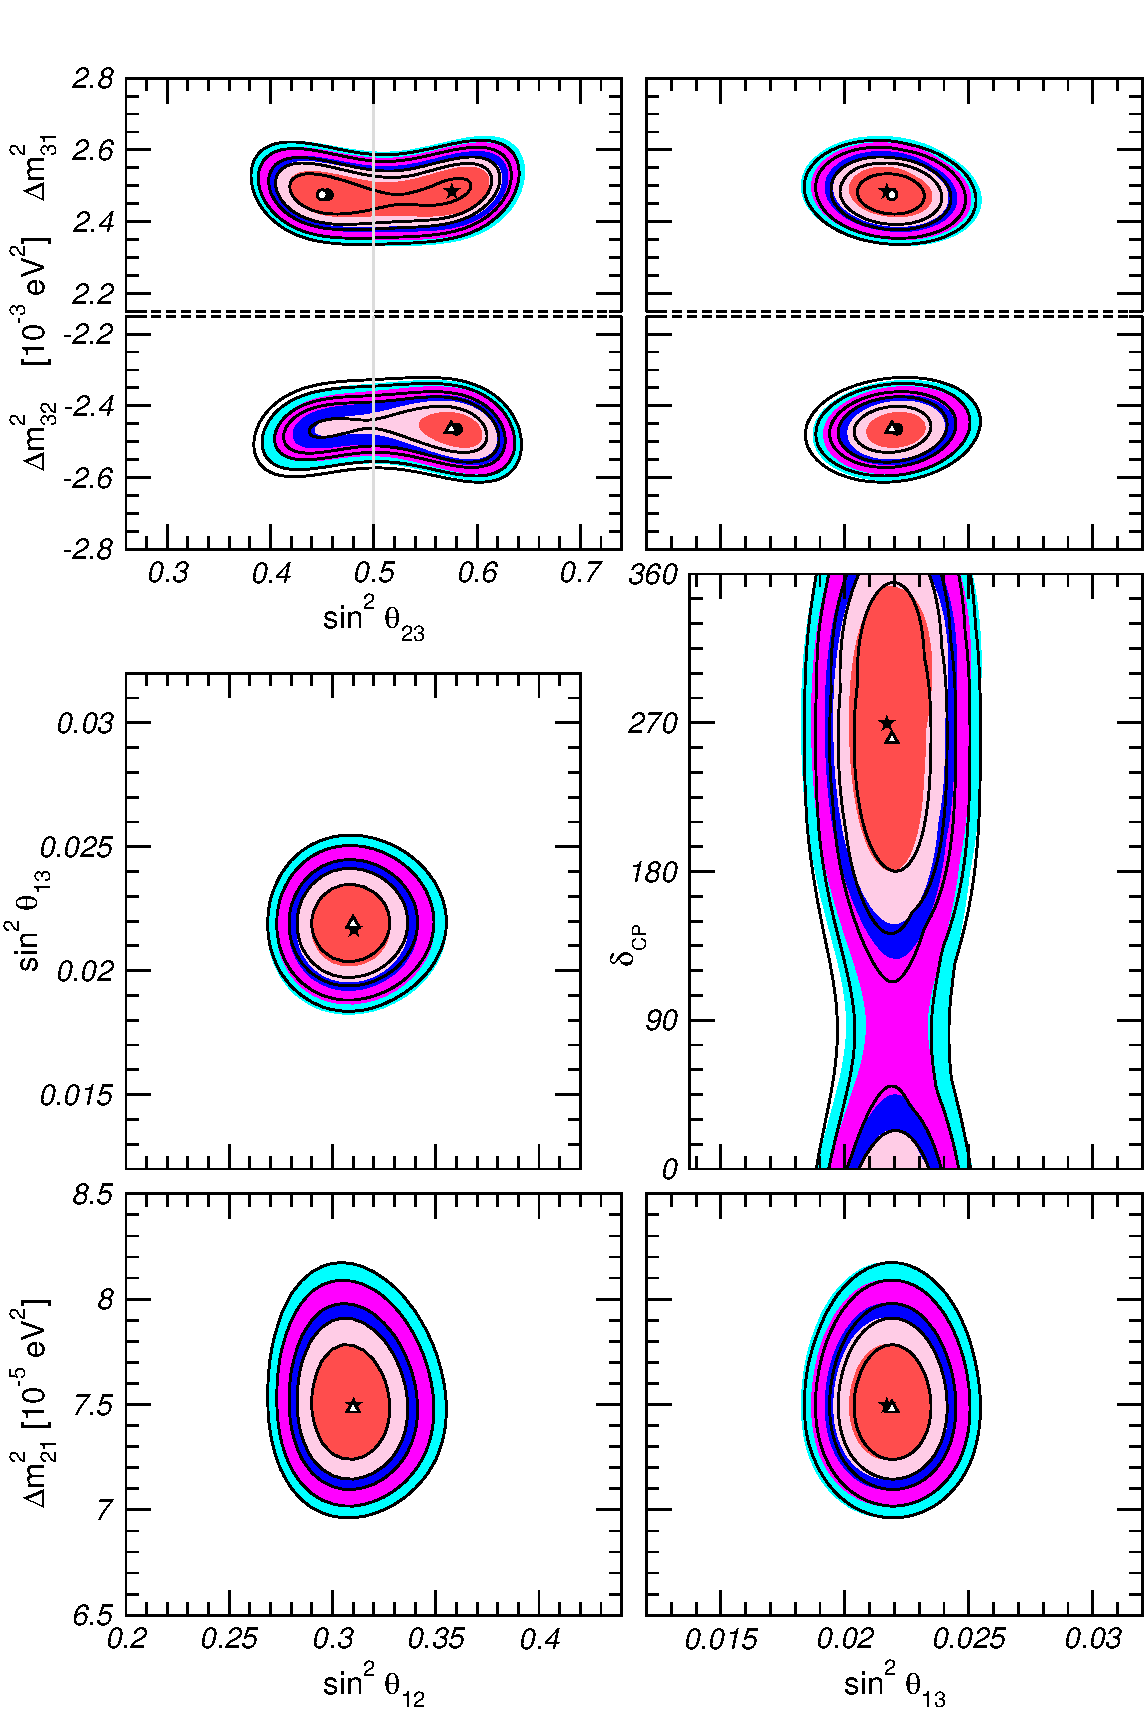
\includegraphics[width=12cm]{GlobalFit.pdf}
  \caption{Global 3-neutrino oscillation analysis taken from \cite{NuFit2014,NuFit2017}. Each panel shows the two-dimensional projection of the allowed six-dimensional region after marginalisation with respect to the undisplayed parameters. The different contours correspond to 1$\sigma$, 90\%, 2$\sigma$, 99\%, 3$\sigma$ CL (2 dof).}
  \label{fig:GlobalFit}
\end{figure}

The value of $\theta_{13}$ was known, from limits determined from global fits to world data, to be much smaller than the others and was even consistent with zero.  In addition to the accelerator experiments, reactor neutrino experiments are also sensitive to $\theta_{13}$ via $\bar{\nu}_e$ disappearance and it was these experiments which produced the decisive results first.  Daya Bay \cite{DayaBay2012} in China and RENO \cite{RENO2012} in South Korea found evidence of a non-zero value in 2012.  There is good agreement between these reactor experiments and more recent measurements from T2K \cite{T2Knue2014} and NO$\nu$A \cite{NOvAnue2016}.

A summary of the best known values for all these oscillation parameters is shown in Table \ref{tab:OscillationParameters}.  The CP-violating phase $\delta_{\textnormal{CP}}$ is currently unmeasured and provides a priority for current and future neutrino experiments.  T2K have excluded the CP conservation regions with little statistical significance and currently favours a maximal CP-violation value of $\delta_{\textnormal{CP}} = -\pi/2$ \cite{T2K2017} [{\color{red}NOTE TO ME! Just preprint, may be published by the time I've finished writing this thing!}]; this holds much promise for future experiments.  The octant of $\theta_{23}$, the location of the parameter in either the $> 45^{\circ}$ or $< 45^{\circ}$ octant, is also undetermined and requires high precision measurements; it is possible that the mixing in this sector is `maximal' ($\theta_{23} = 45^{\circ}$).

\begin{table}
  \caption{The current best-fit values for the neutrino oscillation parameters for normal (inverted) hierarchy.  Taken from \cite{NuFit2017}.}
  \label{tab:OscillationParameters}
  \centering
%  \resizebox*{\columnwidth}{!}{
    \begin{tabular}{c c}
      \toprule
      Parameter & Best fit ($\pm 1\sigma$) \\
      \midrule
      $\sin^2{\theta_{12}}$ & $0.306\pm0.012$ \\
      $\sin^2{\theta_{23}}$ & $0.441^{+0.027}_{-0.021}$ ($0.587^{+0.020}_{-0.024}$) \\
      $\sin^2{\theta_{13}}$ & $0.02166\pm0.00075$ ($0.02179\pm0.00076$) \\
      \midrule
      $\Delta m_{12}^2$ [$10^{-5}$~eV$^2$]     & $+7.50^{+0.19}_{-0.17}$ \\
      $|\Delta m_{3\nu}^2|$ [$10^{-3}$~eV$^2$] & $2.524^{+0.039}_{-0.040}$ ($-2.514^{+0.038}_{-0.041}$) \\
      \midrule
      $\delta_{\textnormal{CP}}$ [$^{\circ}$] & $261^{+51}_{-59}$ ($277^{+40}_{-46}$) \\
      \bottomrule
    \end{tabular}
 % }
\end{table}

%----------------------------------------------------------------------------------------------------------------------------------------------------------------------------
\subsection{Neutrino Mass}\label{sec:NeutrinoMass}

Neutrinos in the Standard Model are massless, for no real reason.  However, the observation of neutrino oscillations implies the existence of neutrino mass (the oscillation probabilities, such as Equations \ref{eq:ElectronNeutrinoAppearance} and \ref{eq:MuonNeutrinoDisappearance}, would be zero if there was no mass splitting).  Three active neutrino flavours gives rise to two independent mass splittings, $\Delta m_{12}^2$ and $\Delta m_{32}^2$, as appear in the oscillation probabilities.  Unfortunately, fitting to the oscillation results provides only a handle on the value of these splittings and not the signs, resulting in an ambiguity in the ordering of the mass states.  This can be resolved in the solar sector by utilising the effect of the MSW resonance encountered by neutrinos in the Sun, allowing the sign of $\Delta m_{12}^2$ to be known (it must be positive as otherwise fewer oscillations, not more, will have been observed by SNO and the other solar neutrino experiments).  This leaves two possible `hierarchies', normal and inverted, which are possible given the experimental data.  These mass splittings also do not offer any indication of an absolute mass scale for the neutrino mass states, this must be constrained using other methods and is currently undetermined.  These uncertainties are illustrated in Figure~\ref{fig:MassHierarchy}.

\begin{figure}
  \centering
  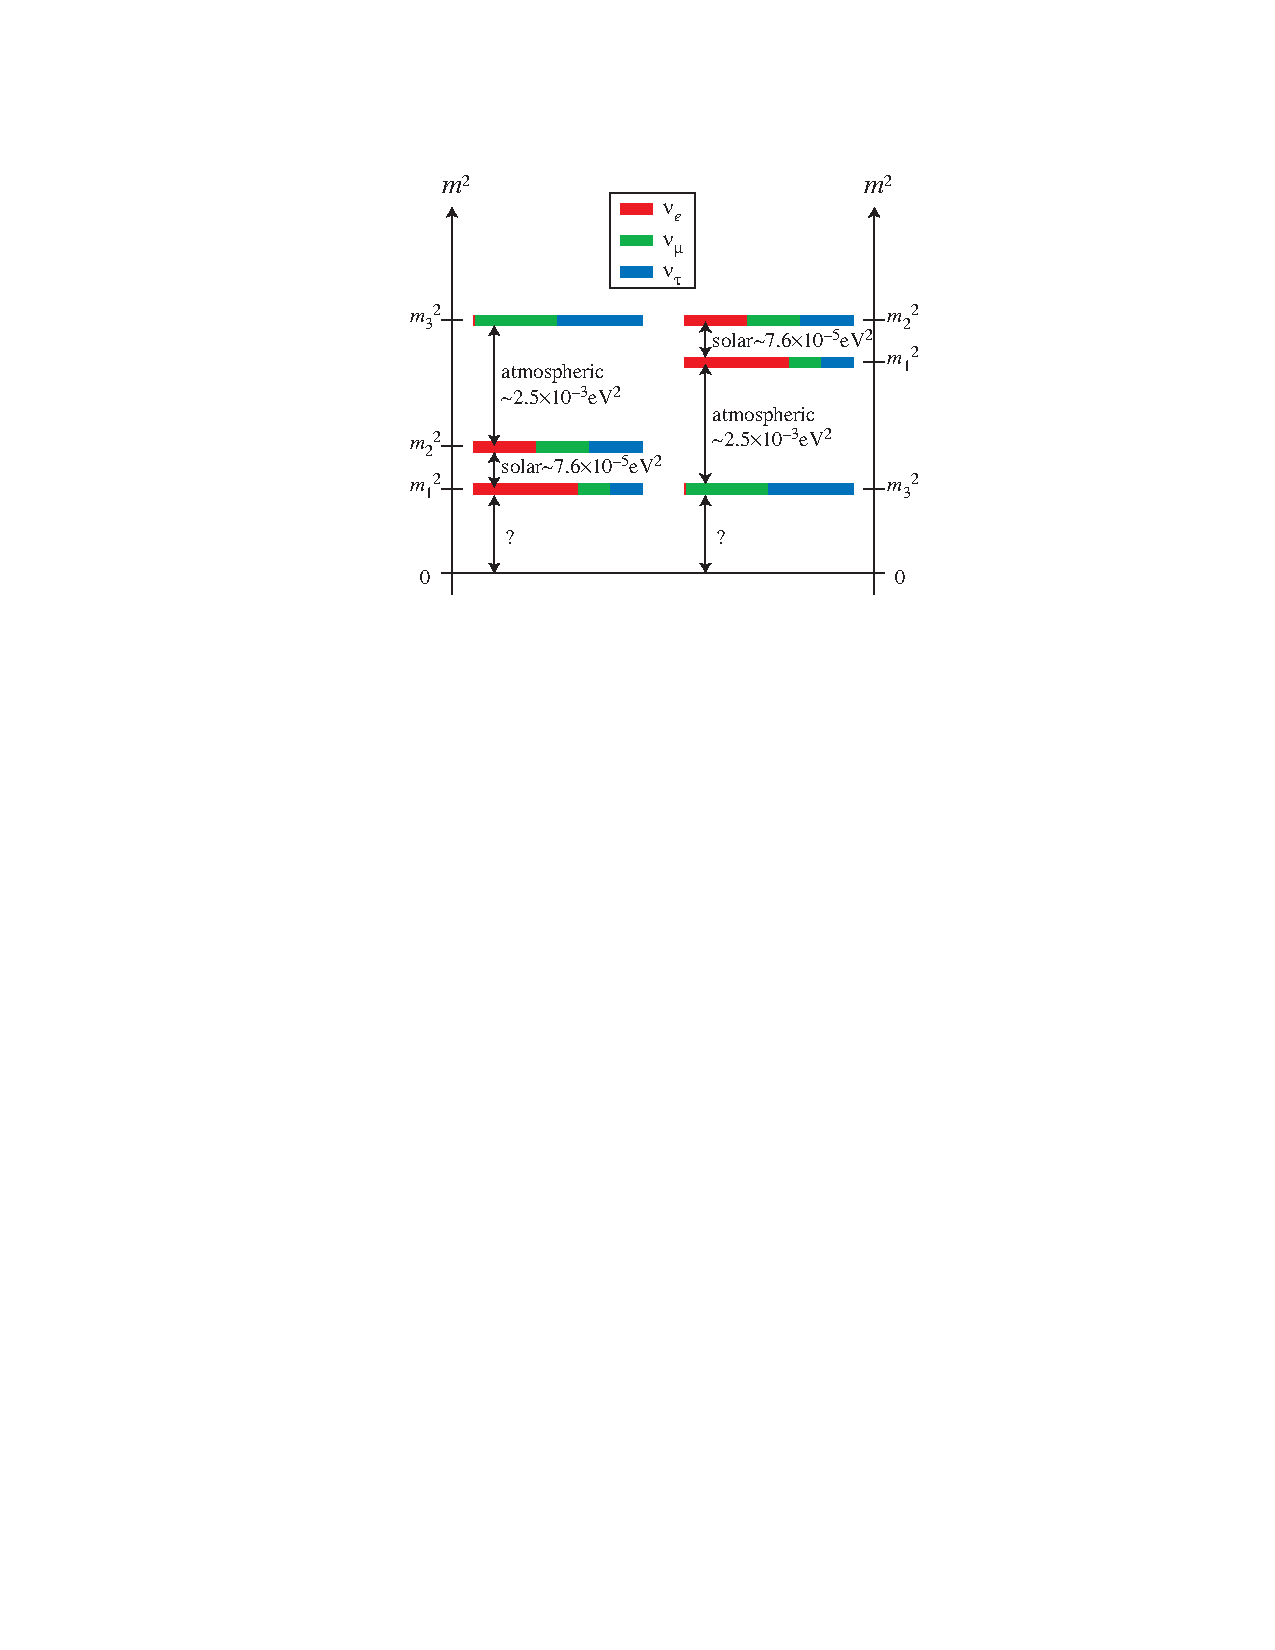
\includegraphics[width=10cm]{MassHierarchy.pdf}
  \caption[Demonstration of the current uncertainties in the neutrino mass.]{Demonstration of the current uncertainties in the neutrino mass.  The undetermined sign in the mass splitting between the 2 and 3 states leaves two possible `hierarchies' open: normal (left figure) and inverted (right figure).  The absolute scale of the masses is also currently unknown.  The flavour composition of each of the mass states, given by the mixing angles, is denoted by the coloured bars.}
  \label{fig:MassHierarchy}
\end{figure}

DUNE will use the MSW effect present as neutrinos propagate through the Earth's crust in order to resolve the hierarchy problem.  It is essential that the hierarchy is resolved since the associated asymmetries between neutrinos and antineutrinos can mimic true CP-violation, which therefore cannot be measured accurately until the mass splittings are completely understood.  Due to the large matter effects associated with its long baseline, the NO$\nu$A experiment is sensitive to the mass hierarchy and may be able to have a say before DUNE and Hyper-Kamiokande.

The absolute neutrino mass cannot be measured from oscillation experiments so other techniques have been developed.  It is possible to use information from $\beta$-decay to get a handle on the mass scale; the $\bar{\nu}_e$ mass alters the spectrum of electrons near the end point so precision measurements can study this effect.  The current best limits on the mass are from H$^3$ $\beta$-decay experiments and yield $m_{\bar{\nu}_e} < 2.05$~eV at 95\% C.L. \cite{Triotsk2011,Mainz2005}.  Cosmological analysis can also constrain the absolute neutrino mass by looking at the distribution of matter in the Universe and information such as galaxy clustering.  The Planck collaboration reported the upper limit on the sum of all neutrino masses as $\sum_i m_{\nu_i} < 0.23$~eV at 95\% C.L. in 2013 \cite{Planck2013}, indicating a significantly lower mass scale than is attainable using current experiments.

%----------------------------------------------------------------------------------------------------------------------------------------------------------------------------
\section{The LAr TPC Concept}\label{sec:LArTPC}

{\color{red} Lee: two things.  Could this be in the DUNE chapter instead?  I like it here I think, but would also work as an introduction to the next chapter.  Also, this should be considered a VERY first draft!  I imagine I will be coming back here often as I write and realise that I assumed something wrt LArTPCs which I had not already explained.  Particularly in the last section, challenges.}

The use of a liquid argon time projection chamber (LArTPC) as a high-precision fine-grained detector medium holds much promise for the successful resolution of the open questions in neutrino physics.  A great amount of R\&D work has taken place to advance the maturity of the technology and pioneering experiments, such as ICARUS \cite{ICARUS2004}, have further increased the understanding of the neutrino community of the detector techniques.  Past and currently running experiments at Fermilab, such as ArgoNeuT \cite{ArgoNeuT2012}, LArIAT \cite{LArIAT2014} and MicroBooNE \cite{MicroBooNE2017}, are successfully using LArTPCs to take and analyse data and it seems certain to be the future of neutrino physics in the U.S. \cite{Baller2014}.

This section will provide a brief history of LArTPC technology and motivate its potential when used in a large experiment such as DUNE.  The basic operation of such a detector will also be described to provide background for discussion of the DUNE and 35~ton experiments, and of reconstruction in LArTPCs, in future chapters.

%----------------------------------------------------------------------------------------------------------------------------------------------------------------------------
\subsection{A Brief History of Time (Projection Chambers)}\label{sec:LArTPCHistory}

The use of a time projection chamber as a potential particle detector was put forward by David Nygren in 1974 \cite{Nygren1974}.  He envisioned bubble-chamber quality data but with the possibility of digital readout of the data, facilitating extremely fine spatial resolution, good timing resolution and fast recovery after triggering.  The basic concept is a drift chamber containing a noble gas placed within a field to drift ionisation electrons created by a propagating particle towards a multielectron array.  This setup allows full three-dimensional reconstruction by combining information from the two-dimensional readout plane with the drift time.  Nygren also included a magnetic field to assist particle identification in his design, shown in Figure~\ref{fig:NygrenTPC}.

\begin{figure}
  \centering
  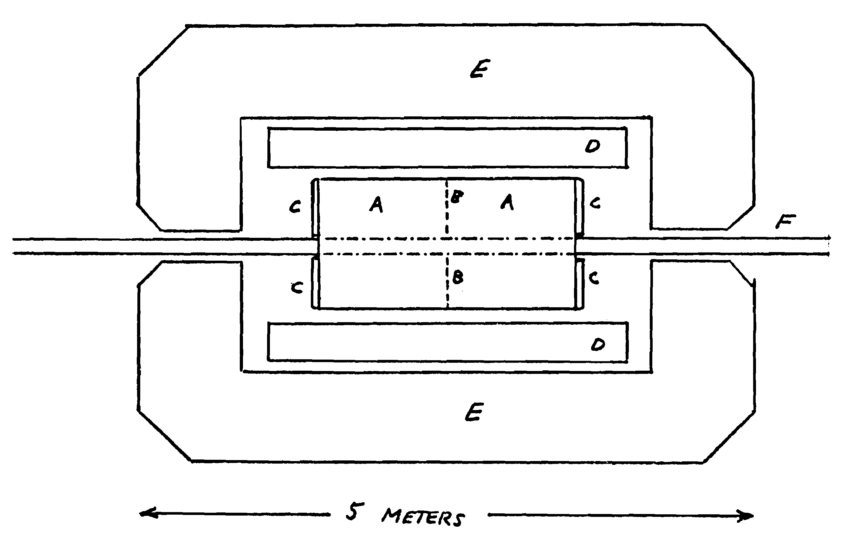
\includegraphics[width=10cm]{NygrenTPC.png}
  \caption[Original TPC design, Nygren (1974)]{The original concept of the time projection chamber particle detector, drawn by David Nygren in 1974 \cite{Nygren1974}.  The sections are labelled as followed: methane-filled region (A), screen to establish electron field (B), end-cap detectors (C), superconducting solenoid (3.33~T) (D), iron return yoke for magnetic field (E), beam vacuum pipe (F).}
  \label{fig:NygrenTPC}
\end{figure}

The extension of this concept to a liquid argon TPC and its potential as a high-precision fine-grained detector medium in neutrino physics was proposed by Carlo Rubbia in 1977 \cite{Rubbia1977}.  The use of a noble liquid rather than gas is necessary in neutrino experiments to provide a high enough target mass for increased probability of neutrino interactions.  Noble liquids have high electron mobility and low diffusion, favourable properties as the detection of particles is from the ionisation and scintillation light created by the particles.  Given the necessity of a high electric field in order to drift these electrons to the readout places, excellent dielectric properties are also required; noble liquids possess such qualities.  The properties of liquid argon which make it almost perfect for this use are demonstrated in Table \ref{tab:NobleProperties}.

\begin{table}
  \caption{Properties of noble liquids relevant when considering a TPC medium for a neutrino experiment \cite{Soderberg2008}.}
  \label{tab:NobleProperties}
  \centering
  \begin{tabular}{ l c c c c c c }
    \toprule
     & Water & He & Ne & \color{red} Ar & Kr & Xe \\
    \midrule
    Boiling point [K] @ 1 atm & 373 & 4.2 & 27.1 & \color{red} 87.3 & 120.0 & 165.0 \\
    Density [g/cm$^3$] & 1 & 0.125 & 1.2 & \color{red} 1.4 & 2.4 & 3.0 \\
    Radiation length [cm] & 36.1 & 755.2 & 24.0 & \color{red} 14.0 & 4.9 & 2.8 \\
    Scintillation [$\gamma$/MeV] & - & 19 000 & 30 000 & \color{red} 40 000 & 25 000 & 42 000 \\
    dE/dx [MeV/cm] & 1.9 & 0.24 & 1.4 & \color{red} 2.1 & 3.0 & 3.8 \\
    Scintillation $\lambda$ [nm] & - & 80 & 78 & \color{red} 128 & 150 & 175 \\
    Natural abundance (Earth atm) [ppm] & $5\times 10^4$ & 5.2 & 18.2 & \color{red} 9340.0 & 1.10 & 0.09 \\
    Electron mobility [cm$^2$/Vs] & low & low & low & \color{red} 400 & 1200 & 2200 \\
    \bottomrule
  \end{tabular}
\end{table}

An additional advantage of this technology is the low threshold for detection; this is set by the ionisation threshold of liquid argon and is only $23.6 \pm 0.5$ eV \cite{Chepel2013}.  Rubbia realised that a LArTPC could be the digital replacement for the high quality particle detection methods used in bubble chambers, very common in neutrino physics in the 1970s.  He proposed the first LArTPC detector design, shown in Figure~\ref{fig:RubbiaLArTPC}, which bears a striking resemblance to the LArTPCs in use today.

\begin{figure}
  \centering
  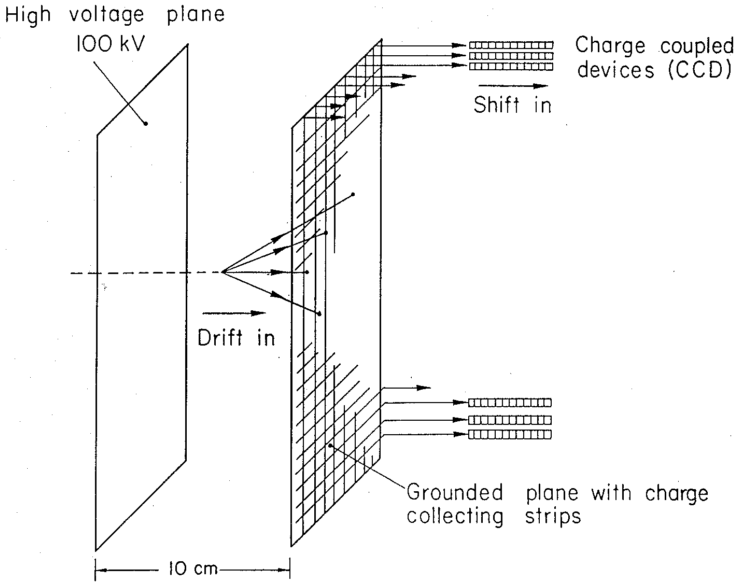
\includegraphics[width=10cm]{RubbiaLArTPC.png}
  \caption[First LArTPC detector, Rubbia (1977)]{The LArTPC detector proposed by Carlo Rubbia in 1977 \cite{Rubbia1977}.}
  \label{fig:RubbiaLArTPC}
\end{figure}

Constructing and operating such a detector was beyond the technology of the time, and is still being understood today.  The operation of a LArTPC detector and the challenges associated with this are the subject of Section \ref{sec:LArTPCOperation}.

%----------------------------------------------------------------------------------------------------------------------------------------------------------------------------
\subsection{LAr TPC Operation}\label{sec:LArTPCOperation}

A LArTPC typically consists of one or more anodes and cathodes at either end of an active drift region.  An ionising particle passing through a LArTPC causes electrons to become free from argon atoms and, in the presence of a field, drift towards an anode where they are read out.

The readout consists of multiple wire planes with different orientations to facilitate the reconstruction.  The wires are either `induction' wires, which allow the electrons to deposit charge but continue past, or `collection' wires, on which the electric field lines end and all the charge on the electron is collected.  Each wire plane is therefore held at a different `bias voltage' to prevent any field lines ending on the induction wire, thus creating local electric fields which promote the continuing forward motion of the electrons.  The signal seen is therefore dependent on the type of wire plane; a bipolar pulse on an induction plane wire and unipolar on a collection plane wire.  It is also common, though not essential, to make use of a `grid plane' upstream of the signal planes in order to shield them from the electron charge until the drift electrons are close.  Without such a plane, the bipolar pulse would be highly asymmetric, though would still have zero integral.  It also makes changing the drift voltage (controlling the electric field) slightly easier as the signal planes are somewhat shielded from its effects.  MicroBooNE does not operate with a grid plane and, although the 35~ton and the DUNE reference design make use of a grid plane, it is uncertain whether the benefit outweighs the cost for a huge LArTPC detector such as the DUNE far detector.  There are alternative readout possibilities to this typical design which have been suggested but, given the scale of future LArTPCs, it is highly unlikely a viable solution which delivers superior readout at a comparable cost will be found.

Upon ionisation, an electron has a certain probability (around 60\%) of recombining before the field can separate it from its ion.  Whilst this compromises the signal observed, it is accompanied by a flash of scintillation light which may be detected and used to assign an `event time' to the interaction, known as T0.  Without this information, it would be impossible to place an absolute time scale on the event and result in an unresolved coordinate along the drift direction.  The magnitude of the applied electric field must be chosen to balance these two effects; a larger field would result in less recombination and therefore compromise the scintillation light while a smaller field would have consequences on the signal received at the wire planes.  Figure~\ref{fig:ElectricFieldScintillationIonisation} demonstrates this and justifies the field value of 500~V/cm which is often chosen in current LAr neutrino experiments.

\begin{figure}
  \centering
  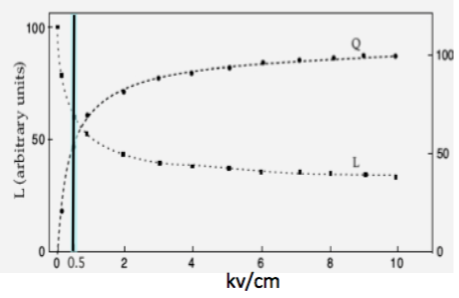
\includegraphics[width=12cm]{ElectricFieldScintillationIonisation.png}
  \caption[Effect of electric field on luminosity of ionisation electrons and scintillation light in a LArTPC.]{Demonstration of the competing effect the electric field has on the luminosity of the ionisation electrons and scintillation light arriving at the detector readout.  Since both are essential in reconstructing the complete interactions, a balance must be found. [PLACEHOLDER IMAGE].}
  \label{fig:ElectricFieldScintillationIonisation}
\end{figure}

The basic operational principles of a LArTPC is demonstrated in Figure~\ref{fig:LArTPCOperation}.  The specifics of how the ionisation charge and the scintillation light is collected and processed is experiment-specific and will be discussed in the context of DUNE in Chapter \ref{chap:DUNE} and the 35~ton experiment in Chapter \ref{chap:35ton}.  This information is all that is required to fully understand and analyse the interactions occurring in the detector; methods used to reconstruct particles and interactions in LAr will be the subject of Chapter \ref{chap:LArTPCReconstruction}.

\begin{figure}[p]
  \centering
  \begin{subfigure}[t]{0.48\linewidth}
    \centering
    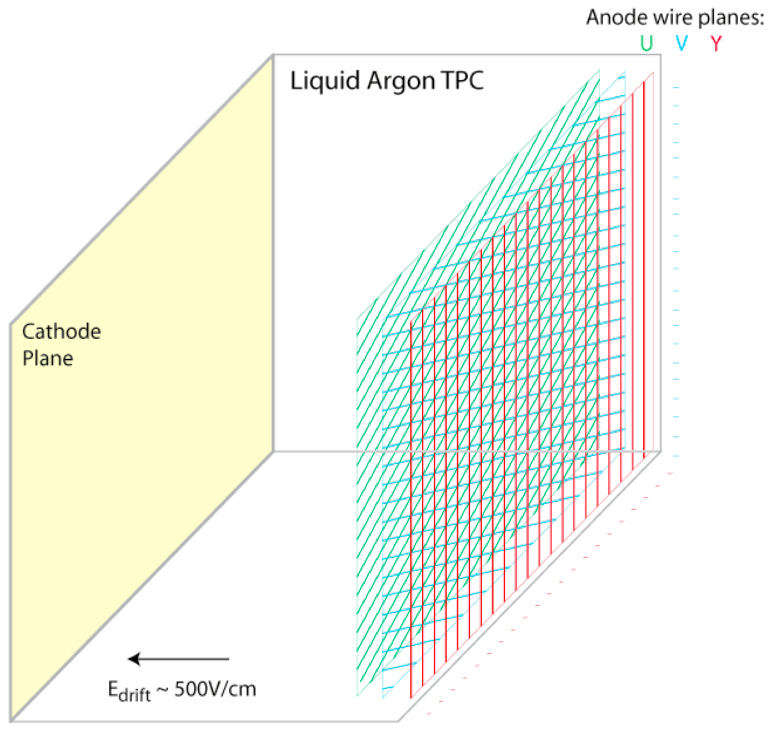
\includegraphics[width=0.98\textwidth]{LArTPCOperation1.png}
    \caption{Typical LArTPC with one cathode (left) and three read out anode planes (right) (two induction, U and V, and one collection, Y), setting up an electric field.  The central region is filled with liquid argon.}
    \label{fig:LArTPCOperation1}
  \end{subfigure}
  \hfill
  \begin{subfigure}[t]{0.48\linewidth}
    \centering
    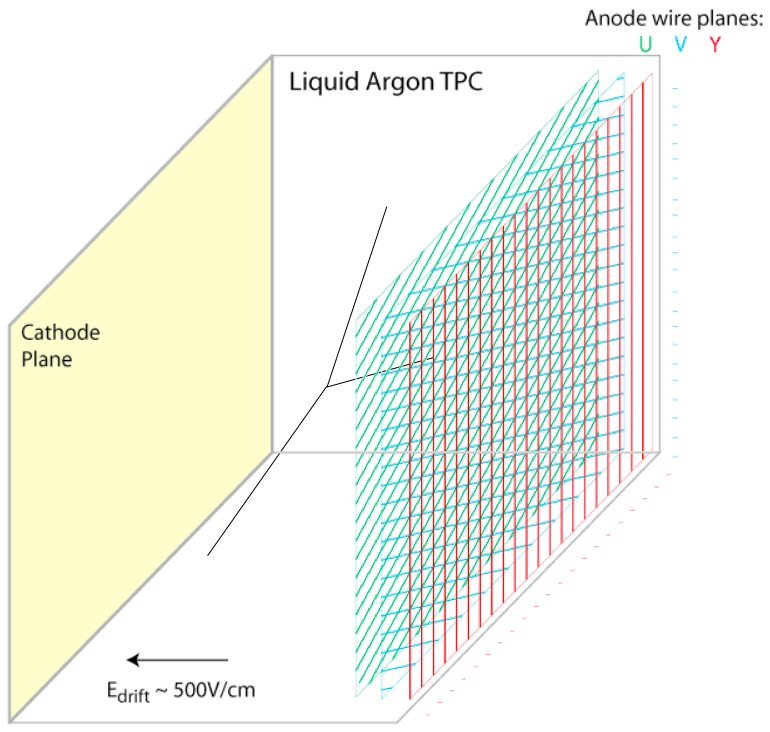
\includegraphics[width=0.98\textwidth]{LArTPCOperation2.png}
    \caption{An ionising particle enters the detector and liberates electrons from the medium, which then drift towards the anode planes.}
    \label{fig:LArTPCOperation2}
  \end{subfigure}
  \hfill
    \begin{subfigure}[t]{0.48\linewidth}
    \centering
    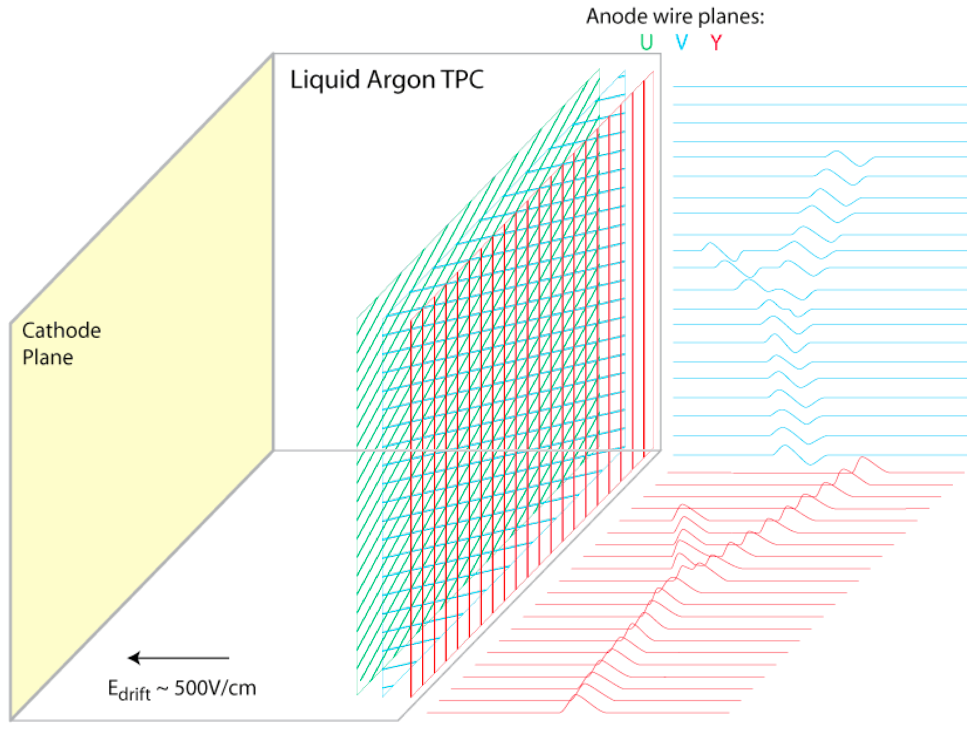
\includegraphics[width=0.98\textwidth]{LArTPCOperation3.png}
    \caption{As the electrons drift through, charge is induced on the first two wire planes and collected on the final one.  Due to the differing orientations of the wires between planes, three complementary views of the interaction are provided (two are shown).}
    \label{fig:LArTPCOperation3}
  \end{subfigure}
  \hfill
  \begin{subfigure}[t]{0.48\linewidth}
    \centering
    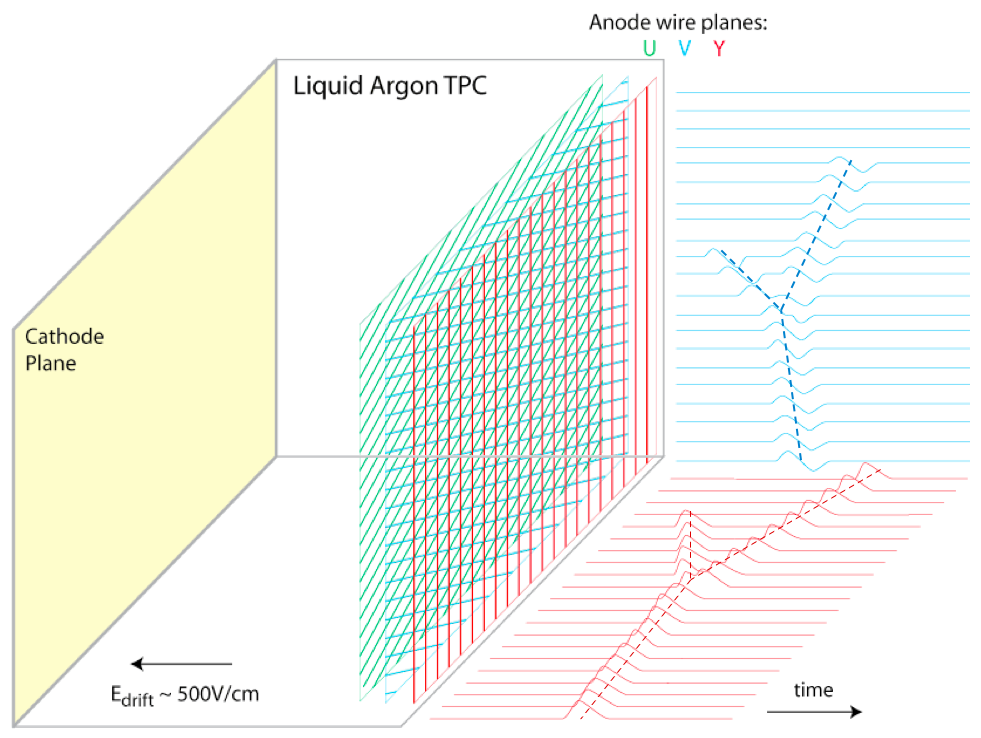
\includegraphics[width=0.98\textwidth]{LArTPCOperation4.png}
    \caption{By combining the two dimensional information provided by the anode planes with the drift time information, the original particle tracks can be inferred.}
    \label{fig:LArTPCOperation4}
  \end{subfigure}
  \caption[Schematic demonstrating the basic operational principles of a LArTPC.]{Schematic demonstrating the basic operational principles of a LArTPC.  The images are stills taken from an illustration created by Bo Yu (BNL) (do I need to cite this?  It's a very common slide and I can't actually find a Bo Yu talk with it in... everyone just puts his name on the slide!).}
  \label{fig:LArTPCOperation}
\end{figure}

%----------------------------------------------------------------------------------------------------------------------------------------------------------------------------
\subsection{LArTPC Challenges}\label{sec:LArTPCChallenges}

There is no doubt of the promise of LArTPCs for the future of neutrino physics but with such expectation comes many challenges.  This will be elaborated upon in more detail when discussing the 35~ton run in Section \ref{sec:35tonPhaseII} but will be briefly mentioned here for completeness.

Given the drift fields required, and the necessary distances, the associated high voltage on the cathode must be on the order of $\sim$100~kV.  This presents engineering challenges related to the feedthrough and cryostat design but also can lead to dielectric breakdown of the liquid nearby such huge voltages.  The properties of LAr and the design implications must be very well understood to ensure this does not endanger the quality of the detector medium.

The presence of electro-negative impurities in the argon can capture drift electrons as they travel towards the anode planes and hinder the signal observed.  The probability of this recombination is referred to as the `electron lifetime' and is directly affected by the maintained purity of the argon.  DUNE expects a contaminant no greater than \#\# ppm O2 and \#\# ppm N2 [to be filled in when I write the DUNE chapter].  This necessitates a purification system to remove impurities and requires the constant recirculation of the liquid through it.  A liquifier is also necessary to recondense any boiled-off gases at the surface.

Along with the possibility of lost signal through finite electron lifetimes, the electrons may also undergo interactions and drift off course either transversely or longitudinally.  This `diffusion' affects the location and size of the observed signal so must also be well understood.

With so much resting on the success of the DUNE experiment, and considering all these effects which must be understood, prototyping is essential.  The 35~ton prototype was constructed as an attempt to better understand LArTPCs and is the subject of Chapter \ref{chap:35ton}.

% DUNE experiments
% Target length: 20 pages

\chapter{The DUNE Experiment}

% Section of thesis on DUNE 35ton prototype
% Target: 30 pages

\graphicspath{{35ton/Figs/}}

%----------------------------------------------------------------------------------------------------------------------------------------------------------------------------
\chapter{The DUNE 35-ton Prototype}\label{chap:35ton}

The 35-ton is the first experimental prototype of the DUNE far detector design and was briefly introduced in Section~\ref{sec:RoadToDUNE}.  It was originally constructed to demonstrate the unique design features of the LBNE far detector and was the only planned prototype for this experiment.  Following the dissolution of LBNE and the subsequent formation of the DUNE collaboration, the 35-ton has become an integral part of the design and execution of the DUNE far detector design.

As discussed in Section~\ref{sec:LArTPC}, the use of LArTPCs in future long-baseline experiments shows great promise.  To facilitate development of the detector technology, Fermilab has an extensive program of LArTPC experiments culminating in the flagship DUNE project.  Prototyping is essential to the success of DUNE as understanding of how to operate progressively larger detectors evolves.  The strategy is staged, with each subsequent phase building on previous success.

The most pertinent issues facing large-scale LArTPCs concern:
\begin{itemize}
  \item the ability to achieve and maintain the necessary LAr purity for successful data taking;
  \item the design and construction of large underground cryostats.
\end{itemize}
The research and development performed thus far have demonstrated viable solutions to these obstacles and reinforced confidence in the design of the experiment and in the upcoming ProtoDUNE projects.

The outcomes of each of these projects at Fermilab are the subject of this present chapter.  The first of the above issues, regarding LAr purity, is discussed in Section~\ref{sec:MTSLAPD} with reference to the Materials Test Stand and the Liquid Argon Purity Demonstrator.  The second complication, concerning the construction of large underground cryostats, was the main motivation for the 35-ton Phase~I experiment and is the subject of Section~\ref{sec:35tonPhaseI}.  The author had no direct involvement in these earlier prototyping efforts.  The culmination of all these developments involved operating a small scale LArTPC alongside these improvements and was achieved in the 35-ton Phase~II run, discussed in Section~\ref{sec:35tonPhaseII}.  Since this experiment forms the basis for later chapters and was actively worked on by the author, it will be reviewed in much greater detail.  A summary of all this R\&D is presented in Section~\ref{sec:35tonSummary}.

%----------------------------------------------------------------------------------------------------------------------------------------------------------------------------
\section[The Materials Test Stand and Liquid Argon Purity Demonstrator]{The Materials Test Stand and\\Liquid Argon Purity Demonstrator}\label{sec:MTSLAPD}

Work developing LArTPCs for future neutrino experiments began at FNAL in 2007 with a view to eventually facilitating a multi-kton LAr experiment.  Even utilising a modular design, as with the DUNE far detector (Section~\ref{sec:FarDetector}), drift distances on the order of a few metres are realistically required, necessitating a low concentration of electronegative impurities.  Attaining and holding the requisite LAr purity in a huge underground cryostat over many years of running is a considerable challenge addressed by the test stands reviewed in this section.

%----------------------------------------------------------------------------------------------------------------------------------------------------------------------------
\subsection{The Materials Test Stand}\label{sec:MTS}

The Materials Test Stand (MTS) \cite{MTS2006,MTS2009a,MTS2009b,MTS2011} was constructed at FNAL to develop LAr purification techniques and to characterise the effect of various materials on the electron lifetime when submerged in the liquid.  It consists of a small cryostat and two filters containing activated-copper-coated granules and an adsorbent molecular sieve respectively; a schematic of the MTS setup is shown in Figure~\ref{fig:MTS}.  The filters are designed to remove oxygen and water contaminants with functionality similar to that successfully demonstrated by the ICARUS collaboration \cite{ICARUS1993b}.  Oxygen is removed by the copper beads using the chemical reaction
\begin{equation}
  2~\textnormal{Cu} + \textnormal{O}_2 \rightarrow 2~\textnormal{CuO}
\end{equation}
and water molecules are physically trapped in the microporous structure of the sieve.  The filters additionally contain the ability to be regenerated in situ, a necessity when planning a long-running experiment, multi-kton experiment; those used previously were primarily proprietary \cite{ICARUS1993a,ICARUS2006}.

\begin{figure}
  \centering
  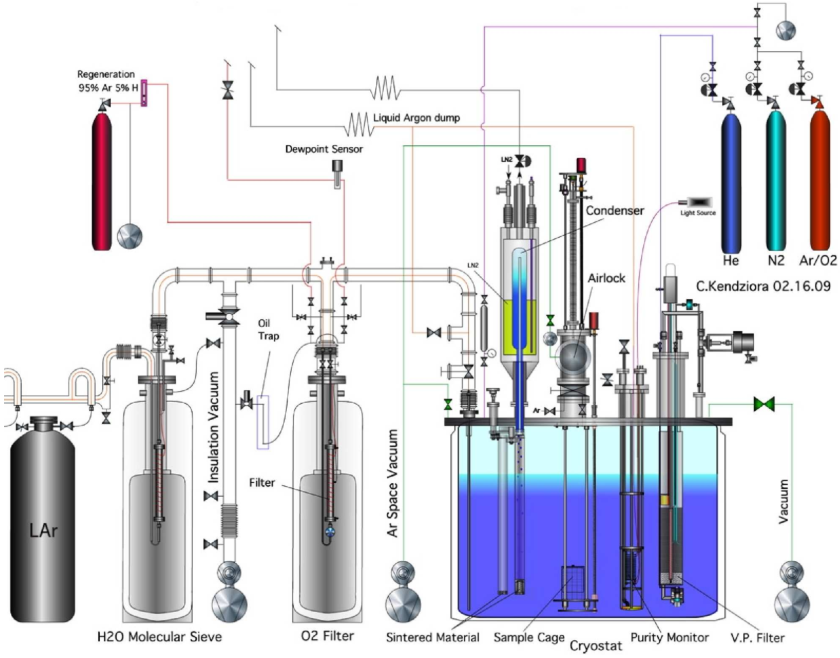
\includegraphics[width=14cm]{MTS.pdf}
  \caption[The Materials Test Stand at FNAL.]{The Materials Test Stand at FNAL \cite{MTS2009b}.  Liquid argon used to fill the cryostat flows from left to right in the schematic, through two filters designed to reduce the H$_2$O and O$_2$ contamination respectively.  A second filter system (the `vapour pump', V.P.), using the same materials, is installed within the cryostat to remove impurities introduced by the materials being examined.}
  \label{fig:MTS}
\end{figure}

The MTS successfully demonstrated good argon purity ($<3$~ppb~H$_2$O) and showed the primary opposition to electron lifetime is water contamination, demonstrated in Figure~\ref{fig:MTSResults}.  It was found that exposure to warm surfaces in the cryostat, such as in the ullage (the volume above the liquid level), facilitated contamination from water impurities as they remain on surfaces even in a vacuum.  The condenser used in the MTS to recondense gaseous argon returned it directly to the liquid in the cryostat (as `raining' condensation) and was found to dramatically reduce the LAr purity when in use.  This is due to contaminants introduced into the gas by exposure to the warm cryostat walls, which could be negated by returning the liquid via a different path which maximised subjection to cold surfaces.  Notably, the electron lifetime was found to be unaffected on the introduction of test materials, although as suspected the temperature of the materials did have an impact.  This is a hugely promising result for the future of LArTPC design and construction.

\begin{figure}
  \centering
  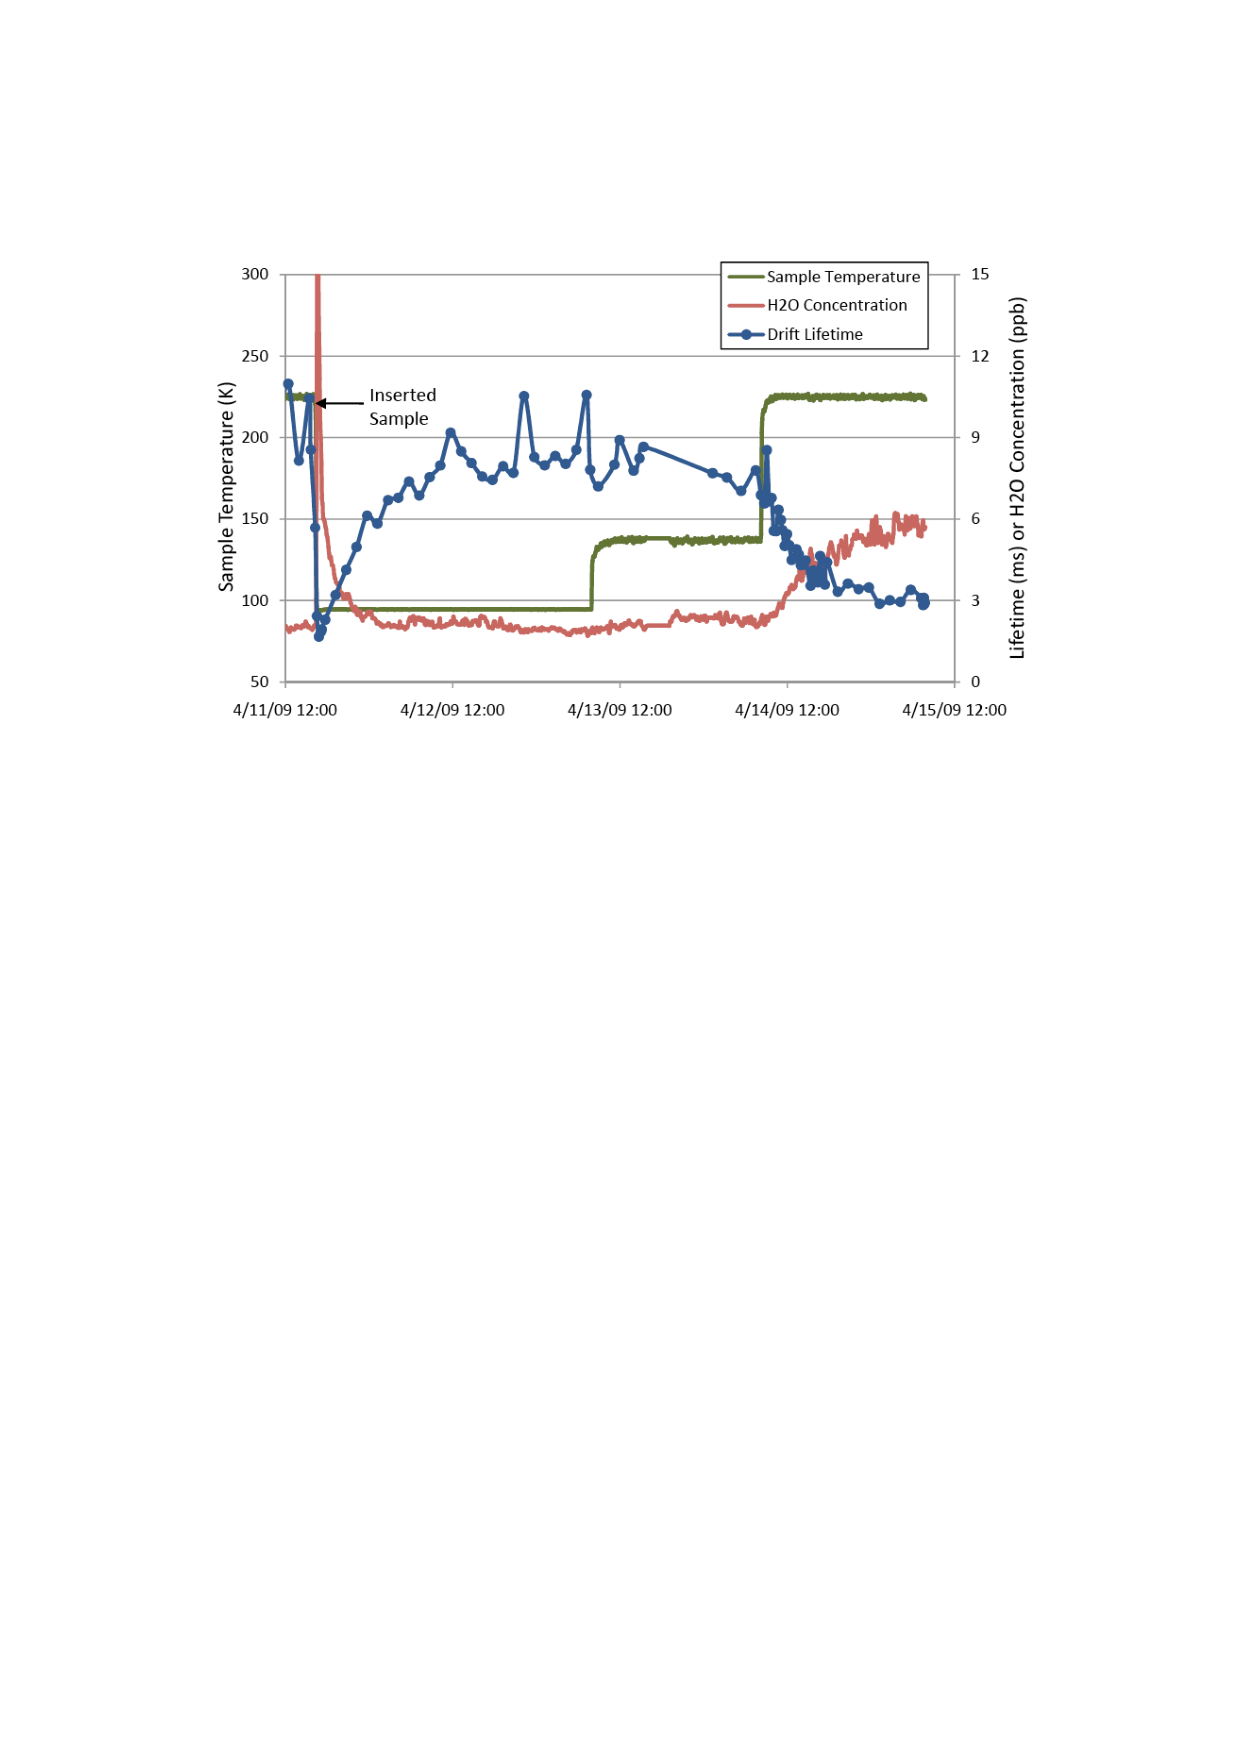
\includegraphics[width=12cm]{MTSResults.pdf}
  \caption[Results from the Materials Test Stand showing the water contamination in LAr and the corresponding electron lifetime.]{Results from the Materials Test Stand showing the water contamination in LAr and the corresponding electron lifetime \cite{MTS2009a}.  There is an obvious inverse correlation between the density of electronegative (H$_2$O) impurities and the resulting lifetime.}
  \label{fig:MTSResults}
\end{figure}

%----------------------------------------------------------------------------------------------------------------------------------------------------------------------------
\subsubsection{Filter Regeneration}\label{sec:FilterRegeneration}

Over time, the filters become less effective as electronegative impurities accumulate.  A significant success of the MTS was demonstrating the process of regenerating the filters in situ.  This is achieved by heating the vessels to 250$^{\circ}$C and, in the case of the molecular sieve, simply using a vacuum pump to remove the water vapour or, in the case of the activated copper, by pumping through a 95:5 mixture of Ar:H$_2$ gas to capture the oxygen through the reduction reaction
\begin{equation}
  \textnormal{CuO} + \textnormal{H}_2 \rightarrow \textnormal{Cu} + \textnormal{H}_2\textnormal{O}.
\end{equation}
During the running of the test stand, the filters were regenerated after the passage of around 1000~litres of liquid argon.  The process takes on the order of a week to heat the filter sufficiently and allow the impurities to be removed; DUNE will utilise replacement modules during this time to ensure continued recirculation.

%----------------------------------------------------------------------------------------------------------------------------------------------------------------------------
\subsubsection{Purity Monitoring}\label{sec:PurityMonitoring}

The ability to constantly evaluate the LAr purity during an experimental run is critically important to ensure high quality data.  The impurity concentrations are typically beyond the capabilities of many conventional gas analysers and so a custom device, known as a `purity monitor' (PrM), is utilised.  The design is based on the purity monitors developed by ICARUS \cite{ICARUSPurityMonitor} and is shown in Figure~\ref{fig:PurityMonitor}.

\begin{figure}
  \centering
  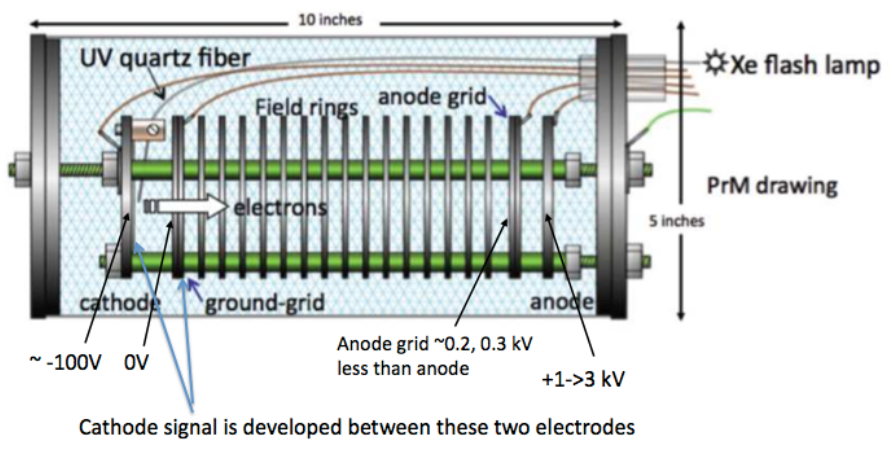
\includegraphics[width=10cm]{PurityMonitor.png}
  \caption[Schematic design of the purity monitors utilised at the FNAL LAr test stands.]{Schematic design of the purity monitors utilised at the FNAL LAr test stands \cite{35tonPhaseI2014}.  Purity monitors using this design were pioneered by ICARUS \cite{ICARUSPurityMonitor} and used in the MTS along with the subsequent Liquid Argon Purity Demonstrator (Section~\ref{sec:LAPD}) and 35-ton Phases~I (Section~\ref{sec:35tonPhaseI}) and~II (Section~\ref{sec:35tonPhaseII}).}
  \label{fig:PurityMonitor}
\end{figure}

The PrM consists of a cylindrical volume containing LAr from its surrounding environment and an anode and photocathode separated by a short drift region.  When taking purity measurements, light from a Xenon flash lamp is incident on the cathode, liberating photoelectrons which traverse towards the anode.  Electronegative impurities in the LAr will decrease the electron lifetime, and therefore the number of electrons reaching a certain point along the drift volume.  A measurement of the ratio of the charge arriving at the anode to that at the cathode is hence a measurement of the inherent purity of the liquid.

The MTS cryostat contains a purity monitor and they were subsequently used in the Liquid Argon Purity Demonstrator and the 35-ton.  When developed for the Liquid Argon Purity Demonstrator and 35-ton cryostats, two sizes were used; long (47~cm) and short (16~cm).

%----------------------------------------------------------------------------------------------------------------------------------------------------------------------------
\subsection{The Liquid Argon Purity Demonstrator}\label{sec:LAPD}

The Liquid Argon Purity Demonstrator (LAPD) \cite{MTS2011,LAPD2014,LAPDJINST2014} was designed to demonstrate the required purity of LArTPC experiments is possible without the use of large scale vacuum pumps.  Previous and current LArTPC experiments, such as ICARUS, ArgoNeuT, LArIAT and MicroBooNE, have been constructed as flat plane vessels and have used an evacuation method as the first step in removing atmospheric impurities to facilitate the required LAr purity.  The necessary mechanical capability of the cryostat to withstand this process, along with the associated equipment, results in unfeasible engineering challenges and costs as detectors increase to multi-kton scales.

In order to circumvent these issues, a design utilising multiple smaller-scale cryostats was proposed.  This however leads to greater complexity relating to both the engineering requirements of the piping infrastructure and the reconstruction capabilities of interactions spanning multiple active volumes.  LAPD successfully pioneered an alternative approach, using a `piston purge' as a first purification step to remove atmospheric impurities.  This is a very important result and has significantly influenced the design of future LArTPC experiments, including the 35-ton.  Additionally, although designed to be evacuated with vacuum pumps, MicroBooNE was filled using the piston purge technique following the success of LAPD.

%----------------------------------------------------------------------------------------------------------------------------------------------------------------------------
\subsubsection{LAPD Experimental Setup}\label{sec:LAPDExperimentalSetup}

The LAPD cryostat is shown in Figure~\ref{fig:LAPD}.  It consists of a cylindrical tank, diameter 10~feet and height 10~feet, with a domed head and a capacity of 32.6~ton LAr.  It is physically next to the MTS and uses the purification system prototyped by this previous effort.  Insulation for the tank is provided by fibreglass sheets covering the outer volume which, along with the tank, is refrigerated by liquid nitrogen (LN$_2$) from an external supply.  As with the MTS, a condenser is utilised above the cryostat to recondense argon gas using coils also cooled with LN$_2$.  This liquid is subsequently sent through the filtration system before being returned to the main volume, a consequence of the previous R\&D with the MTS.  After filling, the system is closed and a good LAr purity is maintained by constant circulation of the cryostat content through the filters.

The system is instrumented with PrMs, gas analysers and temperature sensors.  Four PrMs are contained within the cryostat to measure the purity gradient, with an additional monitor just after the filters to sample to liquid before it is returned to the main volume.  Along with purity, the temperature gradient is measured in order to study the effect of this on electron drift velocity.  The contaminants in the LAr are quantified using nitrogen, oxygen and water analysers outside of the main volume.

\begin{figure}
  \centering
  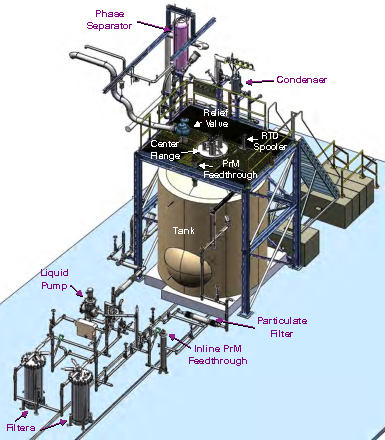
\includegraphics[width=10cm]{LAPD.pdf}
  \caption[The Liquid Argon Purity Demonstrator cryostat and purification system.]{The Liquid Argon Purity Demonstrator cryostat and purification system \cite{LAPDJINST2014}.The two cylinders at the bottom left are the filters described in Section~\ref{sec:MTS}.  The piping facilitates the transport of LAr into and out of the cryostat so continuous purification within a closed system may be achieved.}
  \label{fig:LAPD}
\end{figure}

%----------------------------------------------------------------------------------------------------------------------------------------------------------------------------
\subsubsection{Filling LAPD}\label{sec:FillingLAPD}

The piston purge technique involves injecting warm argon gas at high pressure at the bottom of the cryostat with the top open for venting, demonstrated in Figure~\ref{fig:LAPDPistonPurgeSchematic}.  The heavier than air argon gas acts as a piston, forcing the ambient air out of the top of the cryostat.  Figure~\ref{fig:LAPDPistonPurgeImpurities} demonstrates how this successfully reduces the impurity concentration in the cryostat, shown as a function of complete volume changes.  After completion of the piston purging, the O$_2$ contamination had decreased from 21\% to 6~ppm, N$_2$ from 78\% to 18~ppm and H$_2$O from 200~ppm to 1.2~ppm.

\newsavebox{\largestimage}

\begin{figure}
  \centering
  %\savebox{\largestimage}{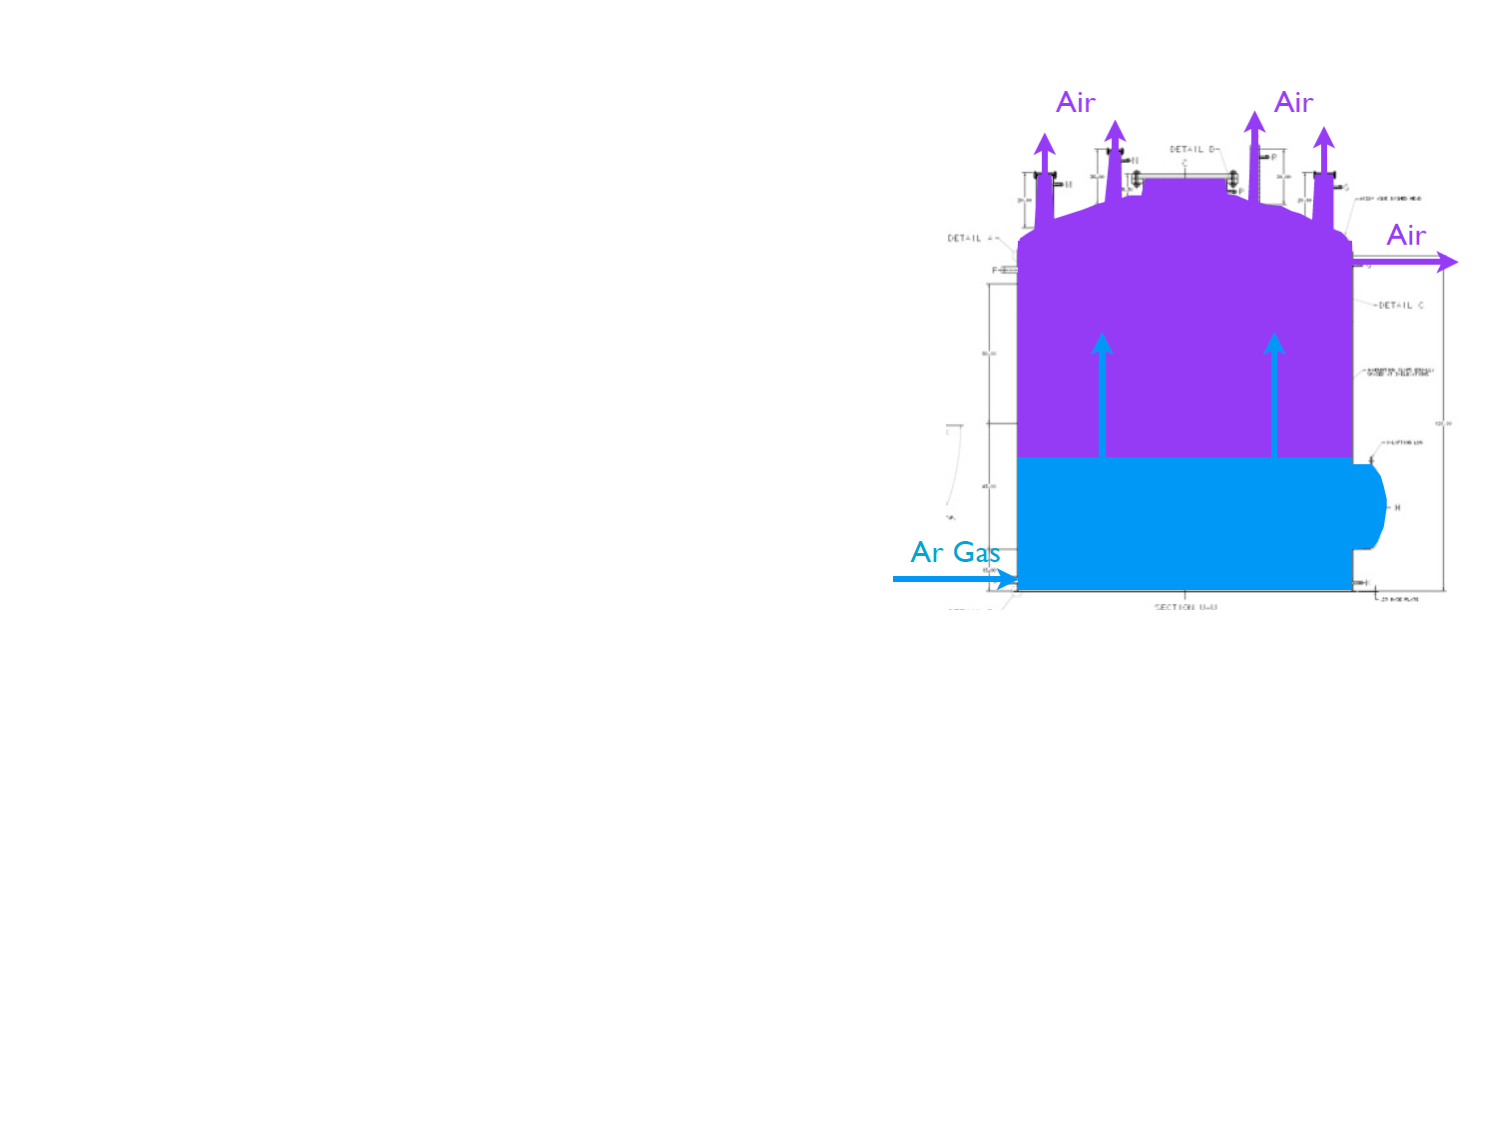
\includegraphics[width=0.49\textwidth]{LAPDPistonPurgeSchematic.pdf}}
  \begin{subfigure}[t]{0.5\linewidth}
    \centering
    %\usebox{\largestimage}
    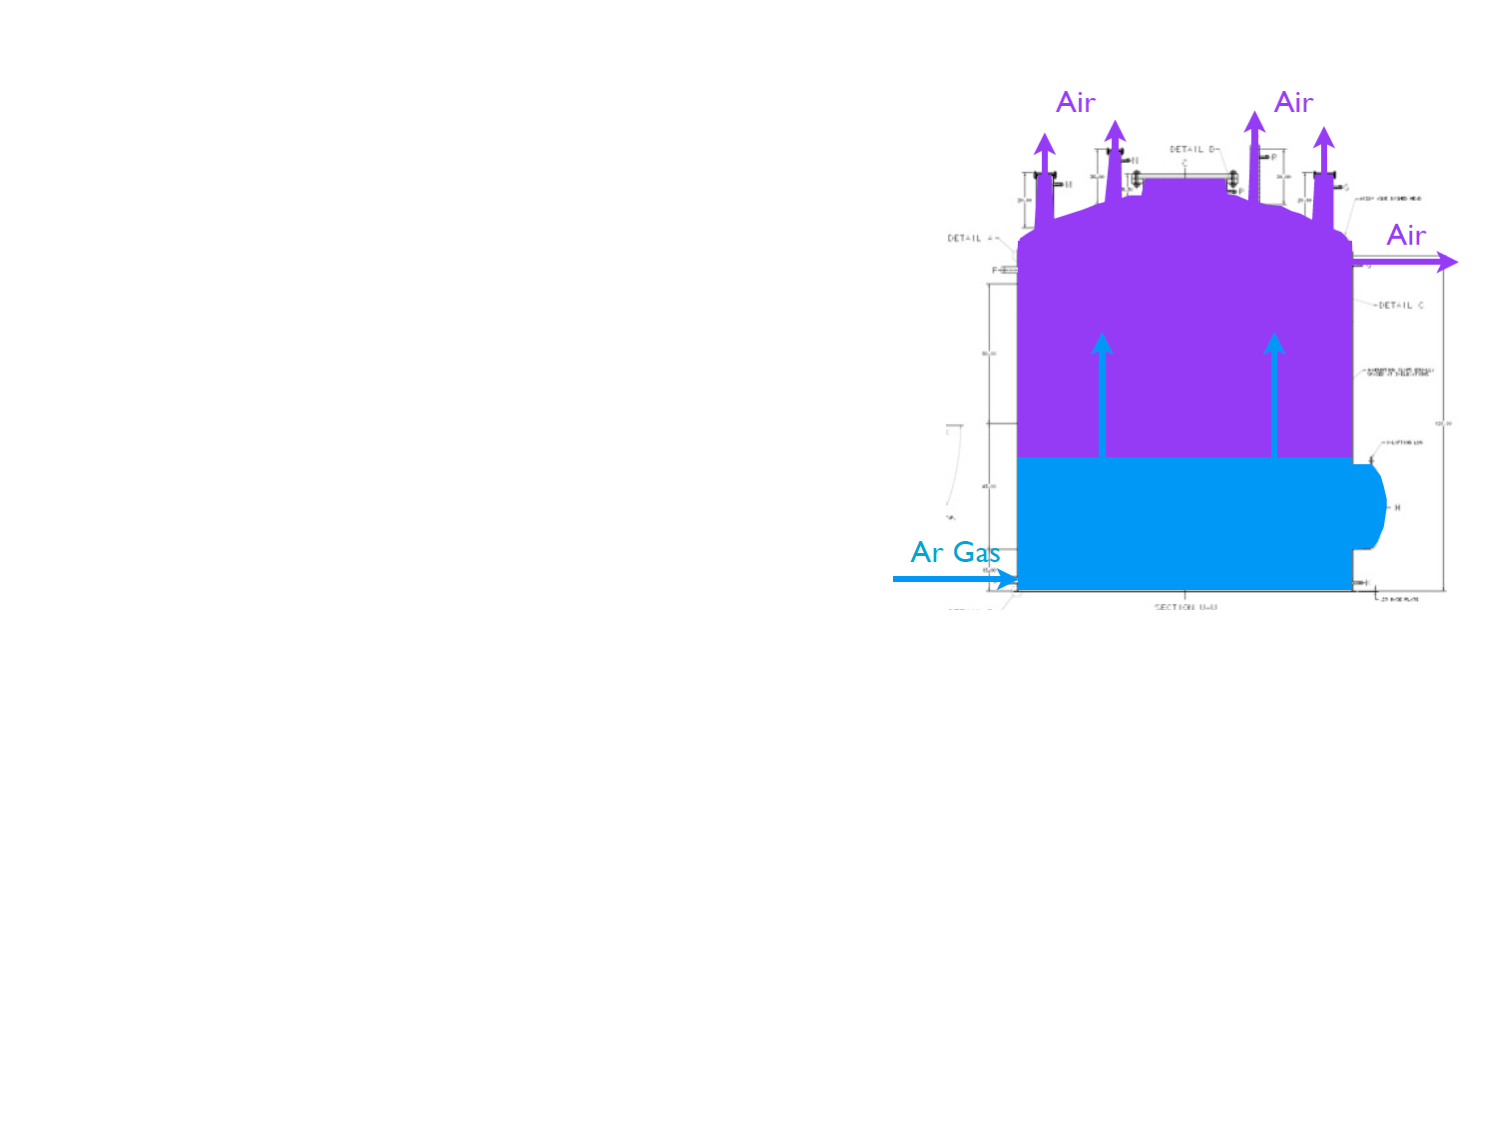
\includegraphics[width=0.98\textwidth]{LAPDPistonPurgeSchematic.pdf}
    \caption{Schematic of the LAPD piston purge.}
    \label{fig:LAPDPistonPurgeSchematic}
  \end{subfigure}\vspace{5mm}
  \begin{subfigure}[t]{0.7\linewidth}
    \centering
    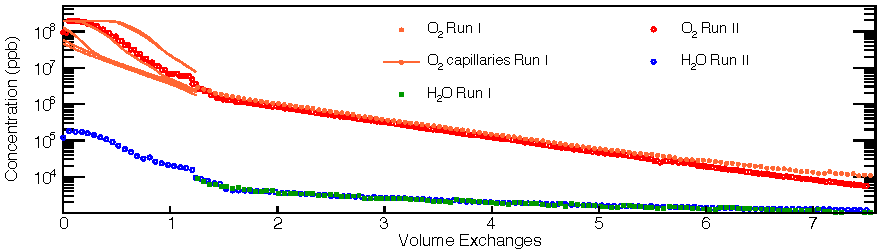
\includegraphics[width=0.98\textwidth]{LAPDPistonPurgeImpurities.pdf}
    %\raisebox{\dimexpr.5\ht\largestimage-.5\height}{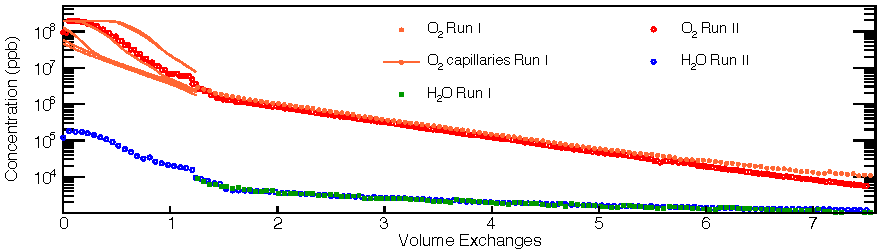
\includegraphics[width=\textwidth]{LAPDPistonPurgeImpurities.pdf}}
    \caption{LAPD impurity concentration during the piston purge.}
    \label{fig:LAPDPistonPurgeImpurities}
  \end{subfigure}
  \caption[The piston purge technique in the Liquid Argon Purity Demonstrator to remove atmospheric impurities before filling.]{The piston purge technique in the Liquid Argon Purity Demonstrator to remove atmospheric impurities before filling \cite{LAPDJINST2014}.  The results from two LAPD runs are shown, the first with the cryostat only half filled to prototype the technique.  Discontinuities between the impurity concentrations are caused by switches between gas analysers.}
  \label{fig:LAPDPistonPurge}
\end{figure}

Following the filling of the cryostat with gaseous argon, the contents are then continuously circulated through the filters to further reduce the impurities present.  The improved electronegative concentrations are shown, again with reference to the number of complete volume changes, in Figure~\ref{fig:LAPDGasCirculation}.  This lasted, as can also be observed in the figure, for a number of days and resulted in a much improved O$_2$ contamination of around 20~ppb and an H$_2$O level which balanced the outgassing rate from the warm cryostat surfaces.

\begin{figure}
  \centering
  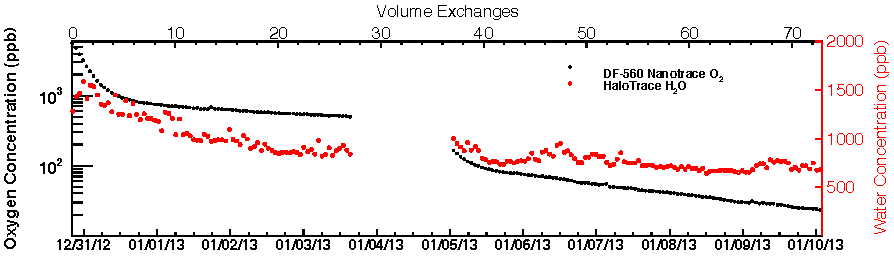
\includegraphics[width=0.7\linewidth]{LAPDGasCirculation.pdf}
  \caption[The concentration of electronegative impurities during the gas circulation stage in the Liquid Argon Purity Demonstrator following the piston purge.]{The concentration of electronegative impurities during the gas circulation stage in the Liquid Argon Purity Demonstrator following the piston purge \cite{LAPDJINST2014}.  The stabilisation of the oxygen contamination signified a leak, which was fixed during the break in readings.}
  \label{fig:LAPDGasCirculation}
\end{figure}

The filling can thus proceed by transporting LAr into the cryostat, through the filter system to ensure a high purity is maintained.  The impurity concentrations were inspected before filling and after filtration and, in total, a volume of 29.7~ton LAr was supplied to the LAPD cryostat.  Once filled, and during the course of operations, the liquid argon volume was constantly recirculated through the filtration system to preserve the LAr purity.  This is shown schematically in Figure~\ref{fig:LAPDLiquidCirculation}.

\begin{figure}
  \centering
  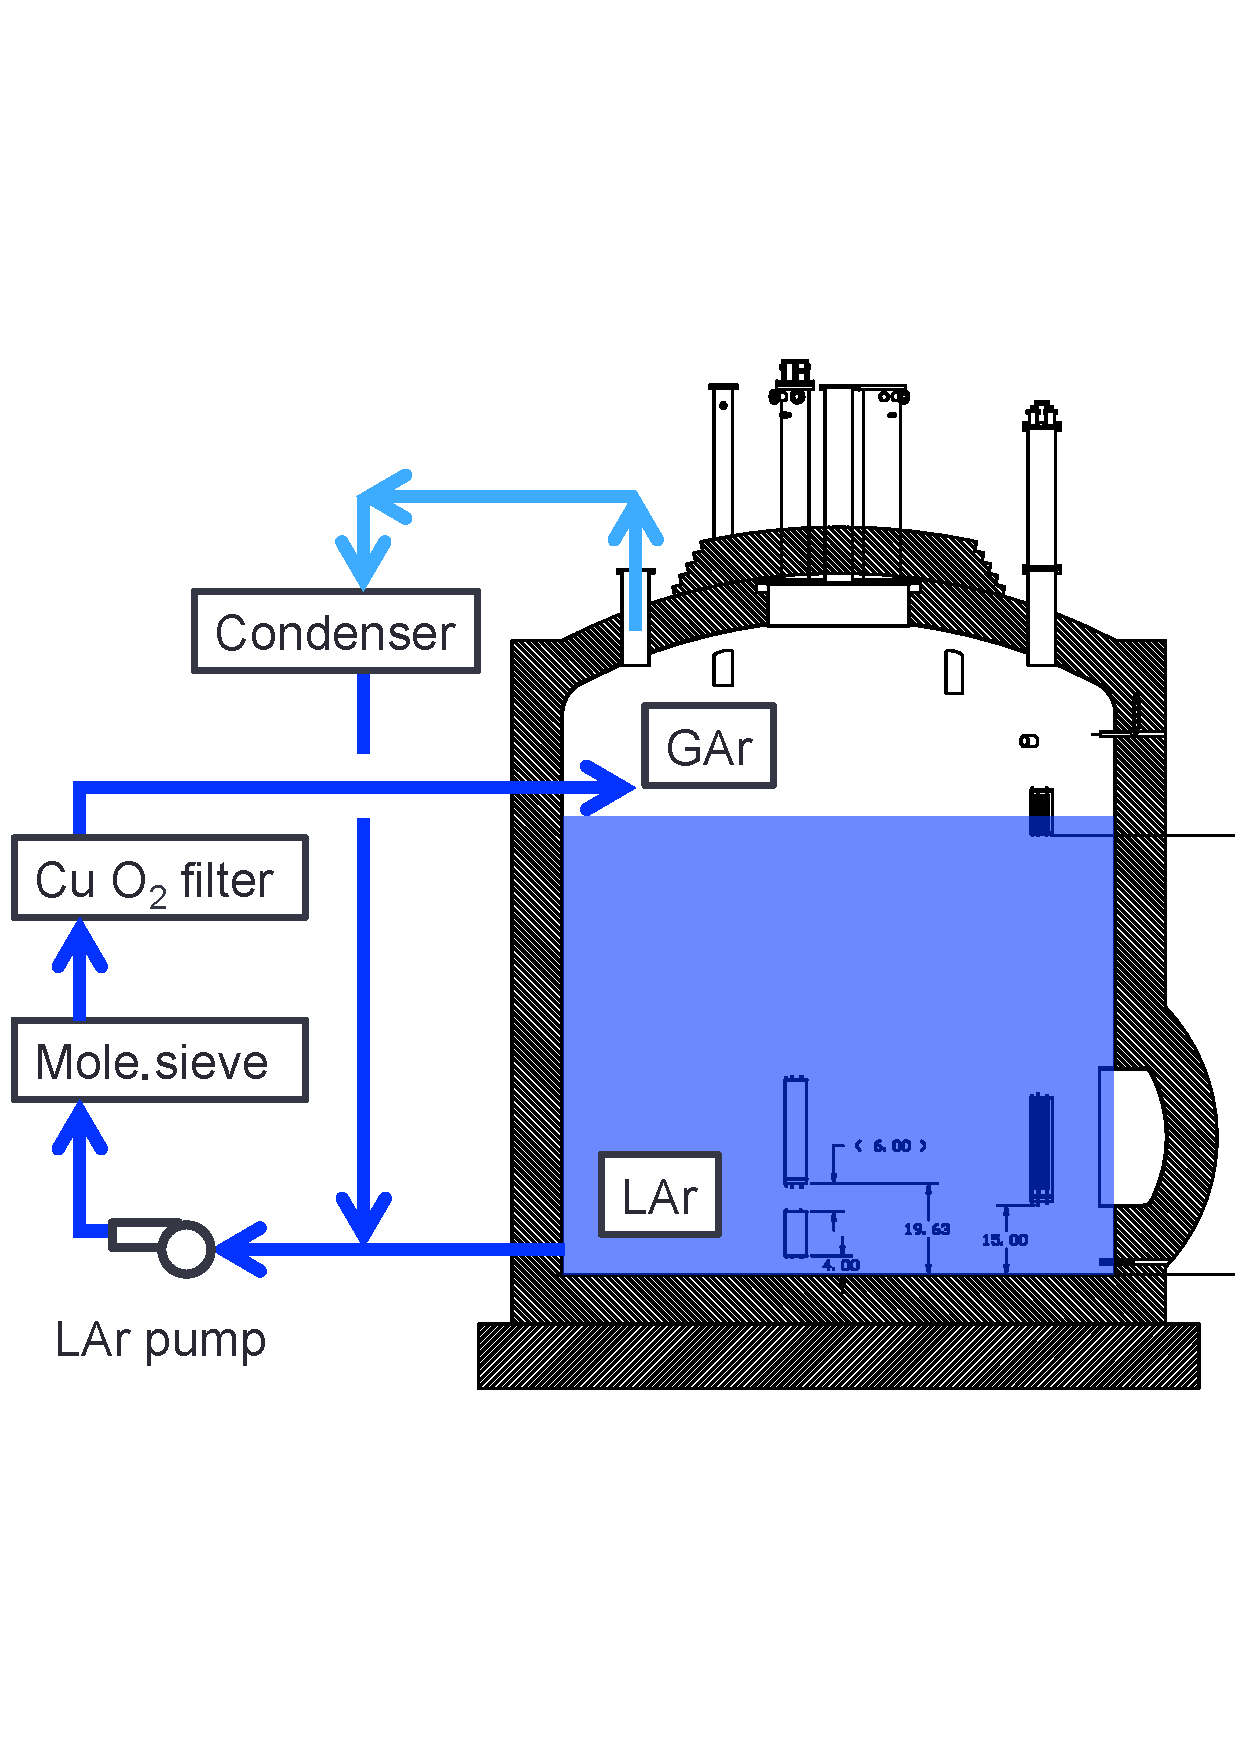
\includegraphics[width=10cm]{LAPDLiquidCirculation.pdf}
  \caption[Schematic showing the recirculation of the LAr during commissioning and operations of the Liquid Argon Purity Demonstrator.]{Schematic showing the recirculation of the LAr during commissioning and operations of the Liquid Argon Purity Demonstrator \cite{LAPD2014}.  Liquid is extracted from the bottom of the cryostat and pumped through the filters to remove any impurities which may have established in the medium.  Following the experience of previous R\&D with the MTS \cite{MTS2009a}, the recondensed liquid is passed through the purification system before being reintroduced to the main volume inside the cryostat.}
  \label{fig:LAPDLiquidCirculation}
\end{figure}

%----------------------------------------------------------------------------------------------------------------------------------------------------------------------------
\subsubsection{LAPD Outcomes}\label{sec:LAPDOutcomes}

LAPD successfully demonstrated achieving and maintaining the required LAr purity for a large neutrino detector is possible without the costly and challenging use of evacuation techniques, reaching purities of better than 60~ppt O$_2$ equivalent.  The measured electron lifetimes over the course of a six week run is shown in Figure~\ref{fig:LAPDElectronLifetime}.  Lifetimes of up to 4~ms were recorded, greater than the DUNE requirement of 3~ms although utilising a much smaller-scale cryostat.  Nonetheless, the success of LAPD has great significance for future LArTPCs, including the 35-ton, and was an important stage in the FNAL LAr test program.

\begin{figure}[ht]
  \centering
  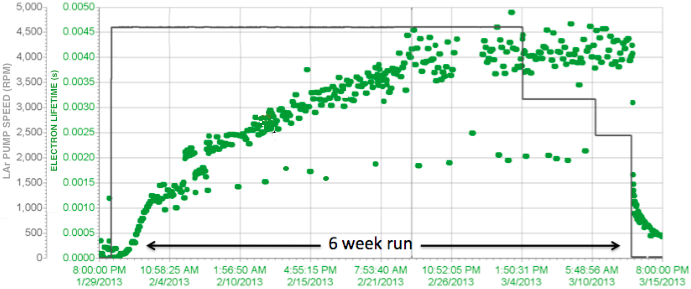
\includegraphics[width=12cm]{LAPDElectronLifetime.png}
  \caption[The electron lifetime achieved in the Liquid Argon Purity Demonstrator during a six week run.]{The electron lifetime achieved in the Liquid Argon Purity Demonstrator during a six week run.  Adapted from \cite{LAPD2014}.}
  \label{fig:LAPDElectronLifetime}
\end{figure}

%----------------------------------------------------------------------------------------------------------------------------------------------------------------------------
\subsection{LongBo}\label{sec:LongBo}

Following the successful LAPD runs, a further phase involved the introduction of a small-scale TPC detector into the liquid argon \cite{LongBo2015}.  The detector is named LongBo (an upgrade from the smaller Bo test detector) and is cylindrical with 25~cm diameter and 2~m length.  It was positioned vertically in the LAPD cryostat, demonstrated in Figure~\ref{fig:LongBo}, and was equipped with a high voltage on the cathode to produce the drift field and three wire planes at the top of the detector for readout.  External scintillator counters were placed around the outer wall of the cryostat to provide triggers on through-going cosmic muons which may deposit charge in the detector.

\begin{figure}
  \centering
  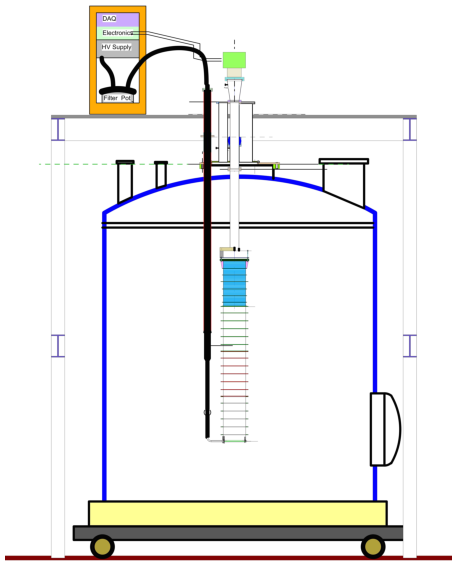
\includegraphics[width=8cm]{LongBo.pdf}
  \caption[The LongBo TPC detector shown within the Liquid Argon Purity Demonstrator Cryostat.]{The LongBo TPC detector shown within the Liquid Argon Purity Demonstrator Cryostat \cite{LongBo2015}.  The black tube represents the high voltage feedthrough to the cathode at the bottom of the TPC.}
  \label{fig:LongBo}
\end{figure}

LongBo was the first LArTPC experiment to utilise `cold readout' electronics to amplify and shape the signal at the front end.  An early version of the ASICs being developed for MicroBooNE were used to read out 16 of the 144 channels, with the remaining using preamplifiers made with discrete circuitry.  At the drift field of 350~V/cm, the signal/noise ratio, a useful number in quantifying the electronics, was around 30, with the channels read out by the ASICs reporting values up to 1.4 times larger.

The LAPD/LongBo experiment successfully maintained similar LAr purities to those without the presence of the detector, as predicted by the results of the MTS.  By using TPC data, it was also possible to make measurements of the purity from through-going muons.  Equation~\ref{eq:ElectronLifetime} may be used to extract a value for the electron lifetime from a plot of deposited charge determined as a function of drift time, where an exponential decay would be expected due to the attenuation from impurities in the LAr.  A comparison between the measured values from the purity monitors and the TPC data may be found in Figure~\ref{fig:LongBoPurity}.  A reasonable agreement is observed between these complimentary measurements, with values between 6~ms and 14~ms reported with 95\% confidence.  These promising results confirmed designing and operating a LArTPC within a non-evacuable cryostat is viable and contributed to the development of the LAr programme towards the DUNE far detector, with the 35-ton experiment the next stage.

\begin{figure}
  \centering
  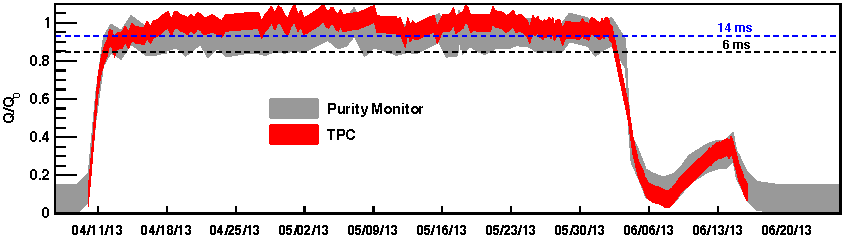
\includegraphics[width=14cm]{LongBoPurity.pdf}
  \caption[The LAr purity within the Liquid Argon Purity Demonstrator cryostat with the LongBo TPC present, measured using both data from the detector and information from the purity monitors.]{The LAr purity within the Liquid Argon Purity Demonstrator cryostat with the LongBo TPC present, measured using both data from the detector and information from the purity monitors \cite{LongBo2015}.  The ratio $Q/Q_0$ is defined as in Equation~\ref{eq:ElectronLifetime}.}
  \label{fig:LongBoPurity}
\end{figure}

%----------------------------------------------------------------------------------------------------------------------------------------------------------------------------
\section{35-ton Experiment: Phase~I}\label{sec:35tonPhaseI}

The scale of the cryostats required for the DUNE experiment are such that constructing them as flat plane vessels 1.5~km underground would be unfeasibly expensive and pose great engineering challenges.  Following the success of LAPD (discussed in Section~\ref{sec:LAPD}), which eliminates the requisite to evacuate the cryostat prior to filling, the LBNE collaboration decided to utilise membrane cryostat technology well established in the liquefied natural gas (LNG) industry.  The 35-ton \cite{35tonPhaseI2014,35tonPhaseI2014Cryostat,35tonPhaseI2015} was therefore employed to demonstrate the application of a membrane cryostat to a LAr experiment.  The DUNE project has maintained this design choice and the 35-ton has since become a recognised and integral part of the collaboration, providing the first test of the technologies envisioned for the eventual far detector.

The 35-ton cryostat was constructed in 2012 at PC4, a former proton facility in a decommissioned beamline at Fermilab.  It has operated in two phases: Phase~I (December 2013 -- February 2014) was proposed to demonstrate the membrane cryostat technology with just the cryostat and purification systems; Phase~II (February 2016 -- April 2016) contained a small-scale DUNE-style detector to validate the integrated system and affirm the detector design elements.  The Phase~I run is the subject of Section~\ref{sec:35tonPhaseI} whilst Phase~II is considered in detail in Section~\ref{sec:35tonPhaseII}.

The 35-ton is the first membrane cryostat used for scientific purposes and the first overall constructed in the United States.  It is also the first designed to contain LAr, which is around three times denser than LNG.  The initial aims of the project (Phase~I) are to demonstrate the feasibility of the cryostat technology for LAr, including thermal performance and leak tightness, and to show the required LAr purity may be achieved without evacuation and maintained through the use of the filtration system developed and validated by the MTS and LAPD.  This first phase will be discussed in this section; the 35-ton cryostat and filling procedures will be described in Sections~\ref{sec:35tonCryostat} and~\ref{sec:35tonFilling} respectively before outcomes of the experiment are presented in Section~\ref{sec:35tonPhaseIOutcomes}.

%----------------------------------------------------------------------------------------------------------------------------------------------------------------------------
\subsection{The 35-ton Cryostat}\label{sec:35tonCryostat}

An overview of the 35-ton cryostat is shown in Figure~\ref{fig:35tonCryostat}.  It contains a concrete shell within which the membrane cryostat is constructed from 2~mm thick stainless steel panels.  An insulated region between these two segments reduces heat leaking.  The roof consists of two plates; Plate A is flat with insulation and membrane beneath and Plate B contains all penetrations and services.  Relevant properties of the 35-ton cryostat are listed in Table~\ref{tab:35tonCryostat}.

\begin{figure}
  \centering
  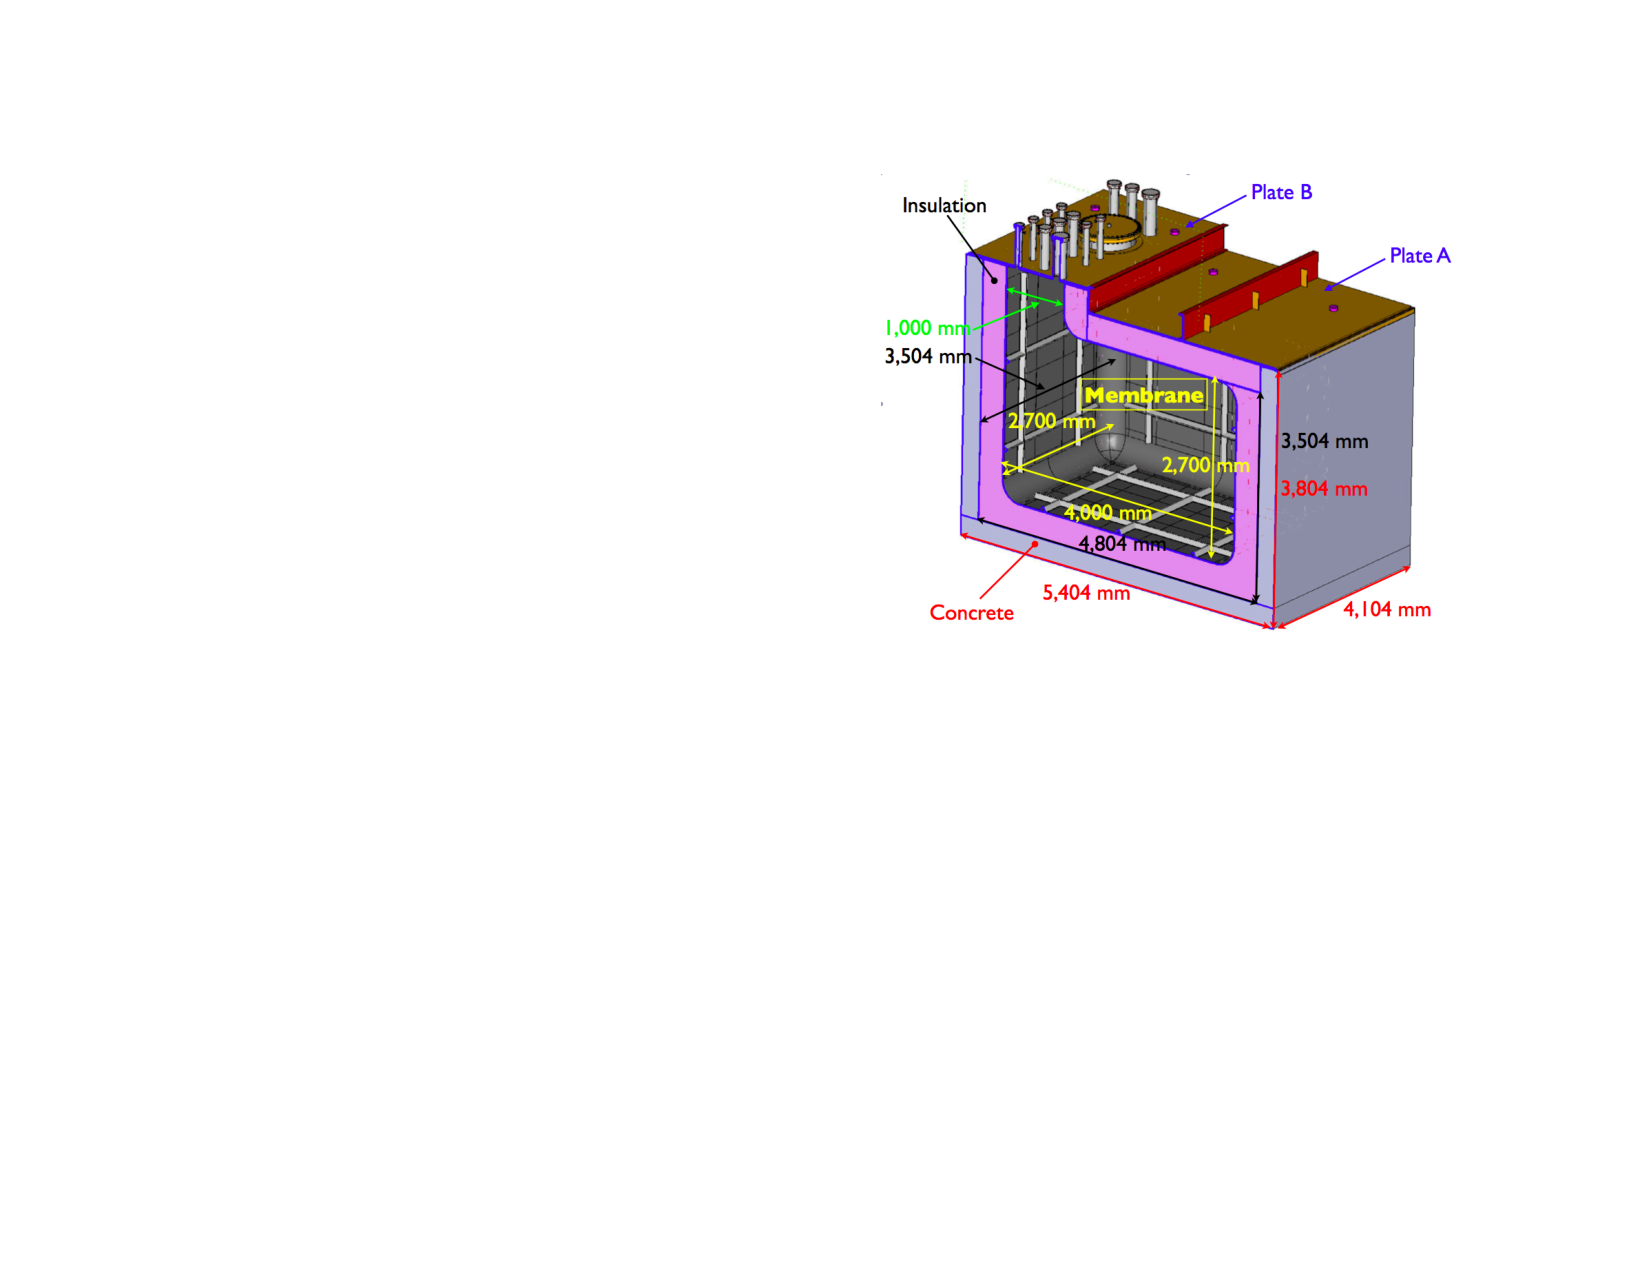
\includegraphics[width=10cm]{35tonCryostat.pdf}
  \caption[The 35-ton cryostat.]{The 35-ton cryostat \cite{35tonPhaseI2015}.}
  \label{fig:35tonCryostat}
\end{figure}

\begin{table}
  \caption[Details and dimensions of the 35-ton cryostat.]{Details and dimensions of the 35-ton cryostat \cite{35tonPhaseI2015}.}
  \label{tab:35tonCryostat}
  \centering
  \begin{tabular}{ l l }
    \toprule
    Parameter & Value \\
    \midrule
    Cryostat volume           & 29.16~m$^3$ \\
    LAr total mass            & 38.6~metric tons \\
    Depth of LAr              & 2.565~m (11\% total ullage) \\
    Inner dimensions          & 4.0~m (length) $\times$ 2.7~m (width) $\times$ 2.7~m (height) \\
    Insulation                & 0.4~m polyurethane foam \\
    Primary membrane          & 2.0~mm thick corrugated stainless steel \\
    Secondary barrier system  & 0.1~mm thick fibreglass \\
    Vapour barrier             & 1.2~mm thick carbon steel \\
    Steel reinforced concrete & 0.3~m thick layer \\
    LAr temperature           & $89\pm1$~K \\
    Operating gas pressure    & 70~mBar \\
    Design pressure           & 207~mBar \\
    Heat leak                 & $<13$~W/m$^2$ \\
    Leak tightness            & $1\times10^{-6}$~mBar$\cdot$litre/s \\
    \bottomrule
  \end{tabular}
\end{table}

The 35-ton was constructed geographically nearby the Liquid Argon Purity Demonstrator in order to utilise existing infrastructure.  It is connected to the LAPD tank, which may be used to store LAr before transfer to the 35-ton, and uses the filtration setup designed and validated by the MTS and LAPD.  This network is shown schematically in Figure~\ref{fig:35tonLAPD}.  Unlike in LAPD, the pumps used in the 35-ton to circulate the LAr through the purification system are within the liquid but the framework operates in a similar way.  An identical condenser is also employed above the cryostat to cool boiled off gaseous argon which is returned to the bottom of the cryostat, near to the pumps which subsequently extract the liquid for purification.  The LAr was circulated at a rate of three volumes per day by the pumps, with the filters designed to remove 2~ppm~O$_2$ from 35~tons of LAr before saturating.  The argon used to fill the cryostat had an initial purity of around 1~ppm~O$_2$ and so the filters were able to operate throughout the planned lifetime of the experiment without the need for regeneration.

\begin{figure}
  \centering
  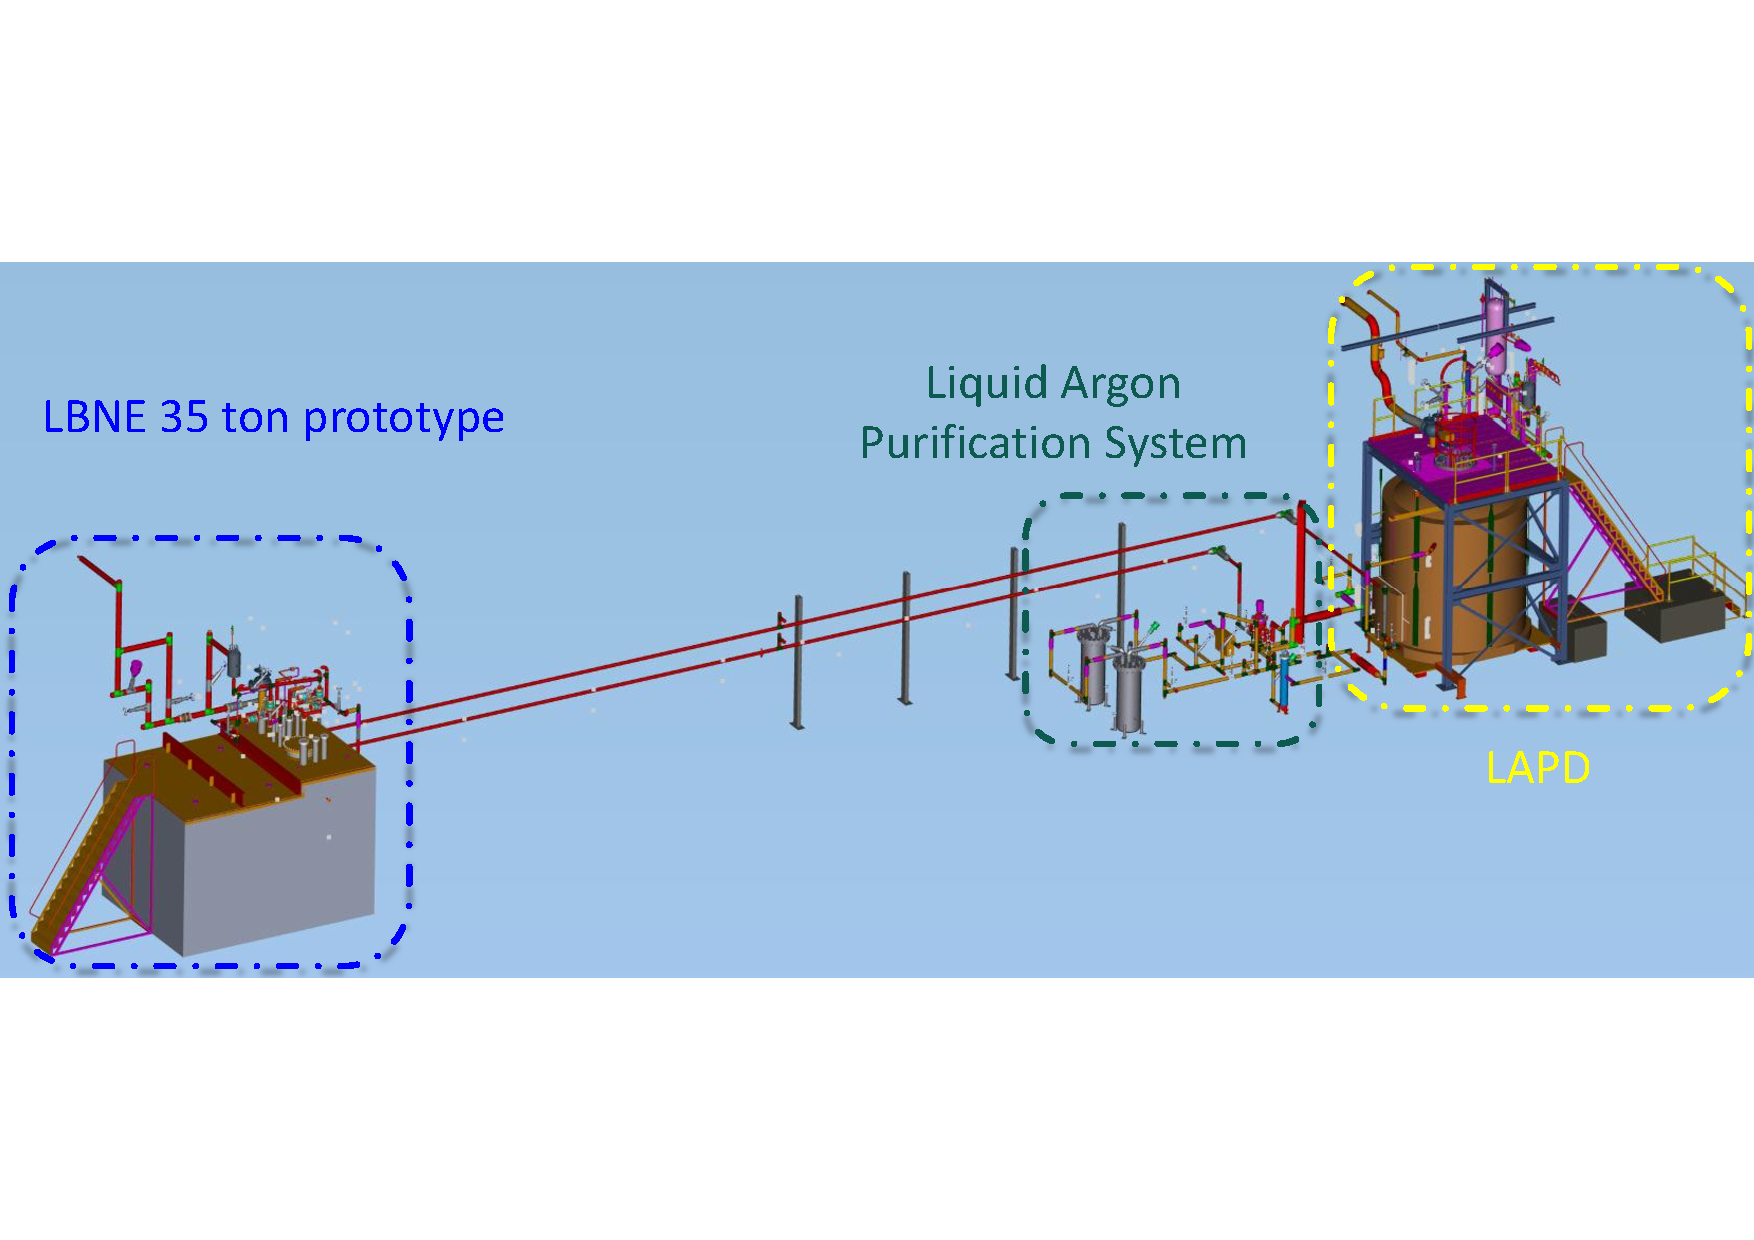
\includegraphics[width=14cm]{35tonLAPD.pdf}
  \caption[The network linking the 35-ton cryostat, the Liquid Argon Purity Demonstrator and the purification system at PC4, Fermilab.]{The network linking the 35-ton cryostat, the Liquid Argon Purity Demonstrator and the purification system at PC4, Fermilab \cite{35tonPhaseI2014}.}
  \label{fig:35tonLAPD}
\end{figure}

The cryogenic environment is monitored and controlled using standard detectors, including temperature sensors, pressure transducers, flow meters and level sensors, along with a suite of commercial gas analysers.  The height of the volume is instrumented with four PrMs, two large and two small, with an additional long monitor positioned after the filters, as with LAPD.  Also as previously, the vertical temperature profile in the cryostat is monitored at 23~cm intervals with temperature detectors suspended on a chain.

%----------------------------------------------------------------------------------------------------------------------------------------------------------------------------
\subsection{Filling the 35-ton}\label{sec:35tonFilling}

The 35-ton cryostat is filled in a similar way to the Liquid Argon Purity Demonstrator, described in Section~\ref{sec:FillingLAPD}.  Initially, a piston purge with warm gaseous argon is performed to remove atmospheric impurities before closing off the vents and redirecting argon at the top of the cryostat through the filters for purification.  The impurity concentrations for this stage of filling are shown in Figure~\ref{fig:35tonGasFilling}.  Before filling with liquid, the cryostat is cooled in an attempt to reduce outgassing and to create an appropriate environment in which to introduce LAr.  This is achieved by injecting LAr through a spray at the top of the cryostat which generates a turbulent mixing of cold gas within the cryostat and gradually cools the walls of the vessel.  Following this, LAr is transferred from LAPD into the 35-ton; since the 35-ton is slightly larger than LAPD, this is conducted in two stages.  The cooldown and LAr filling stages are shown in Figure~\ref{fig:35tonLiquidFilling}.

\begin{figure}
  \centering
  \begin{subfigure}[t]{0.48\linewidth}
    \centering
    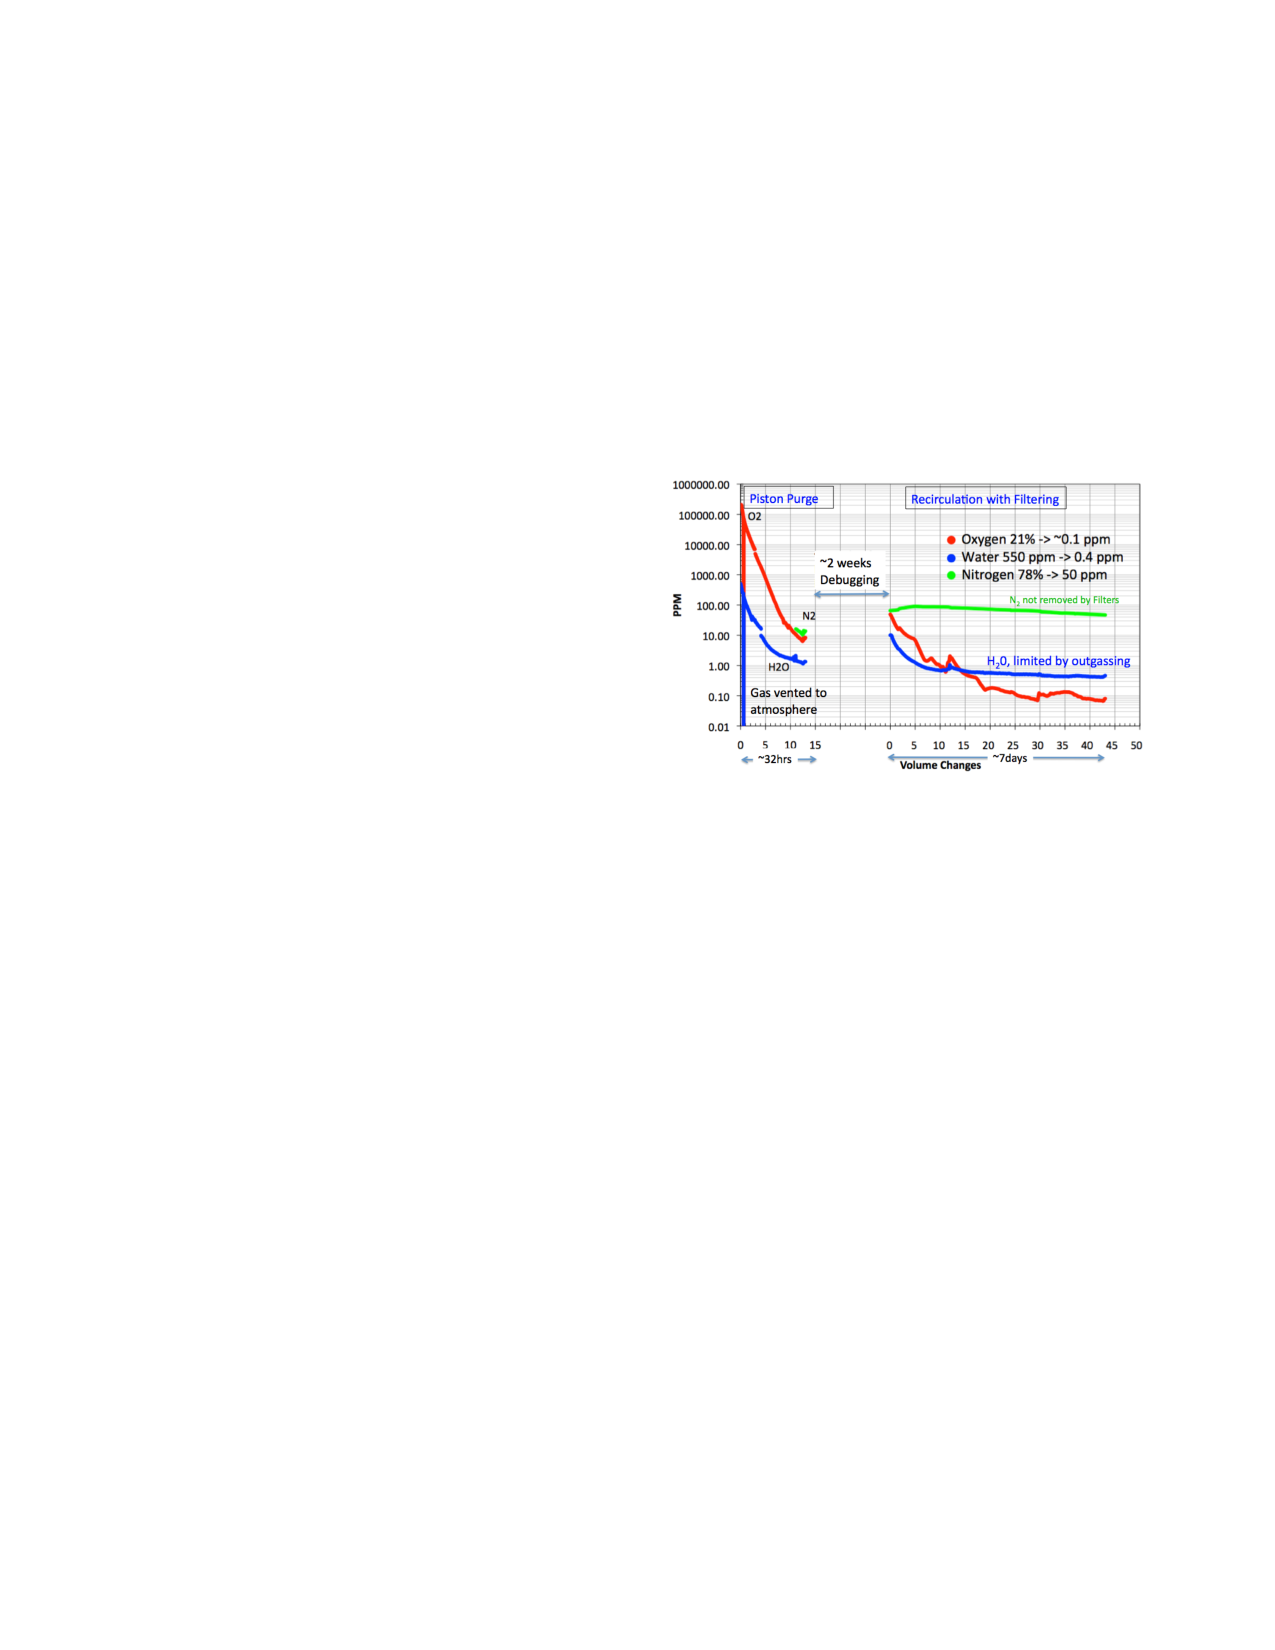
\includegraphics[width=0.98\textwidth]{35tonGasFilling.pdf}
    \caption{Gas filling.}
    \label{fig:35tonGasFilling}
  \end{subfigure}
  \hfill
  \begin{subfigure}[t]{0.48\linewidth}
    \centering
    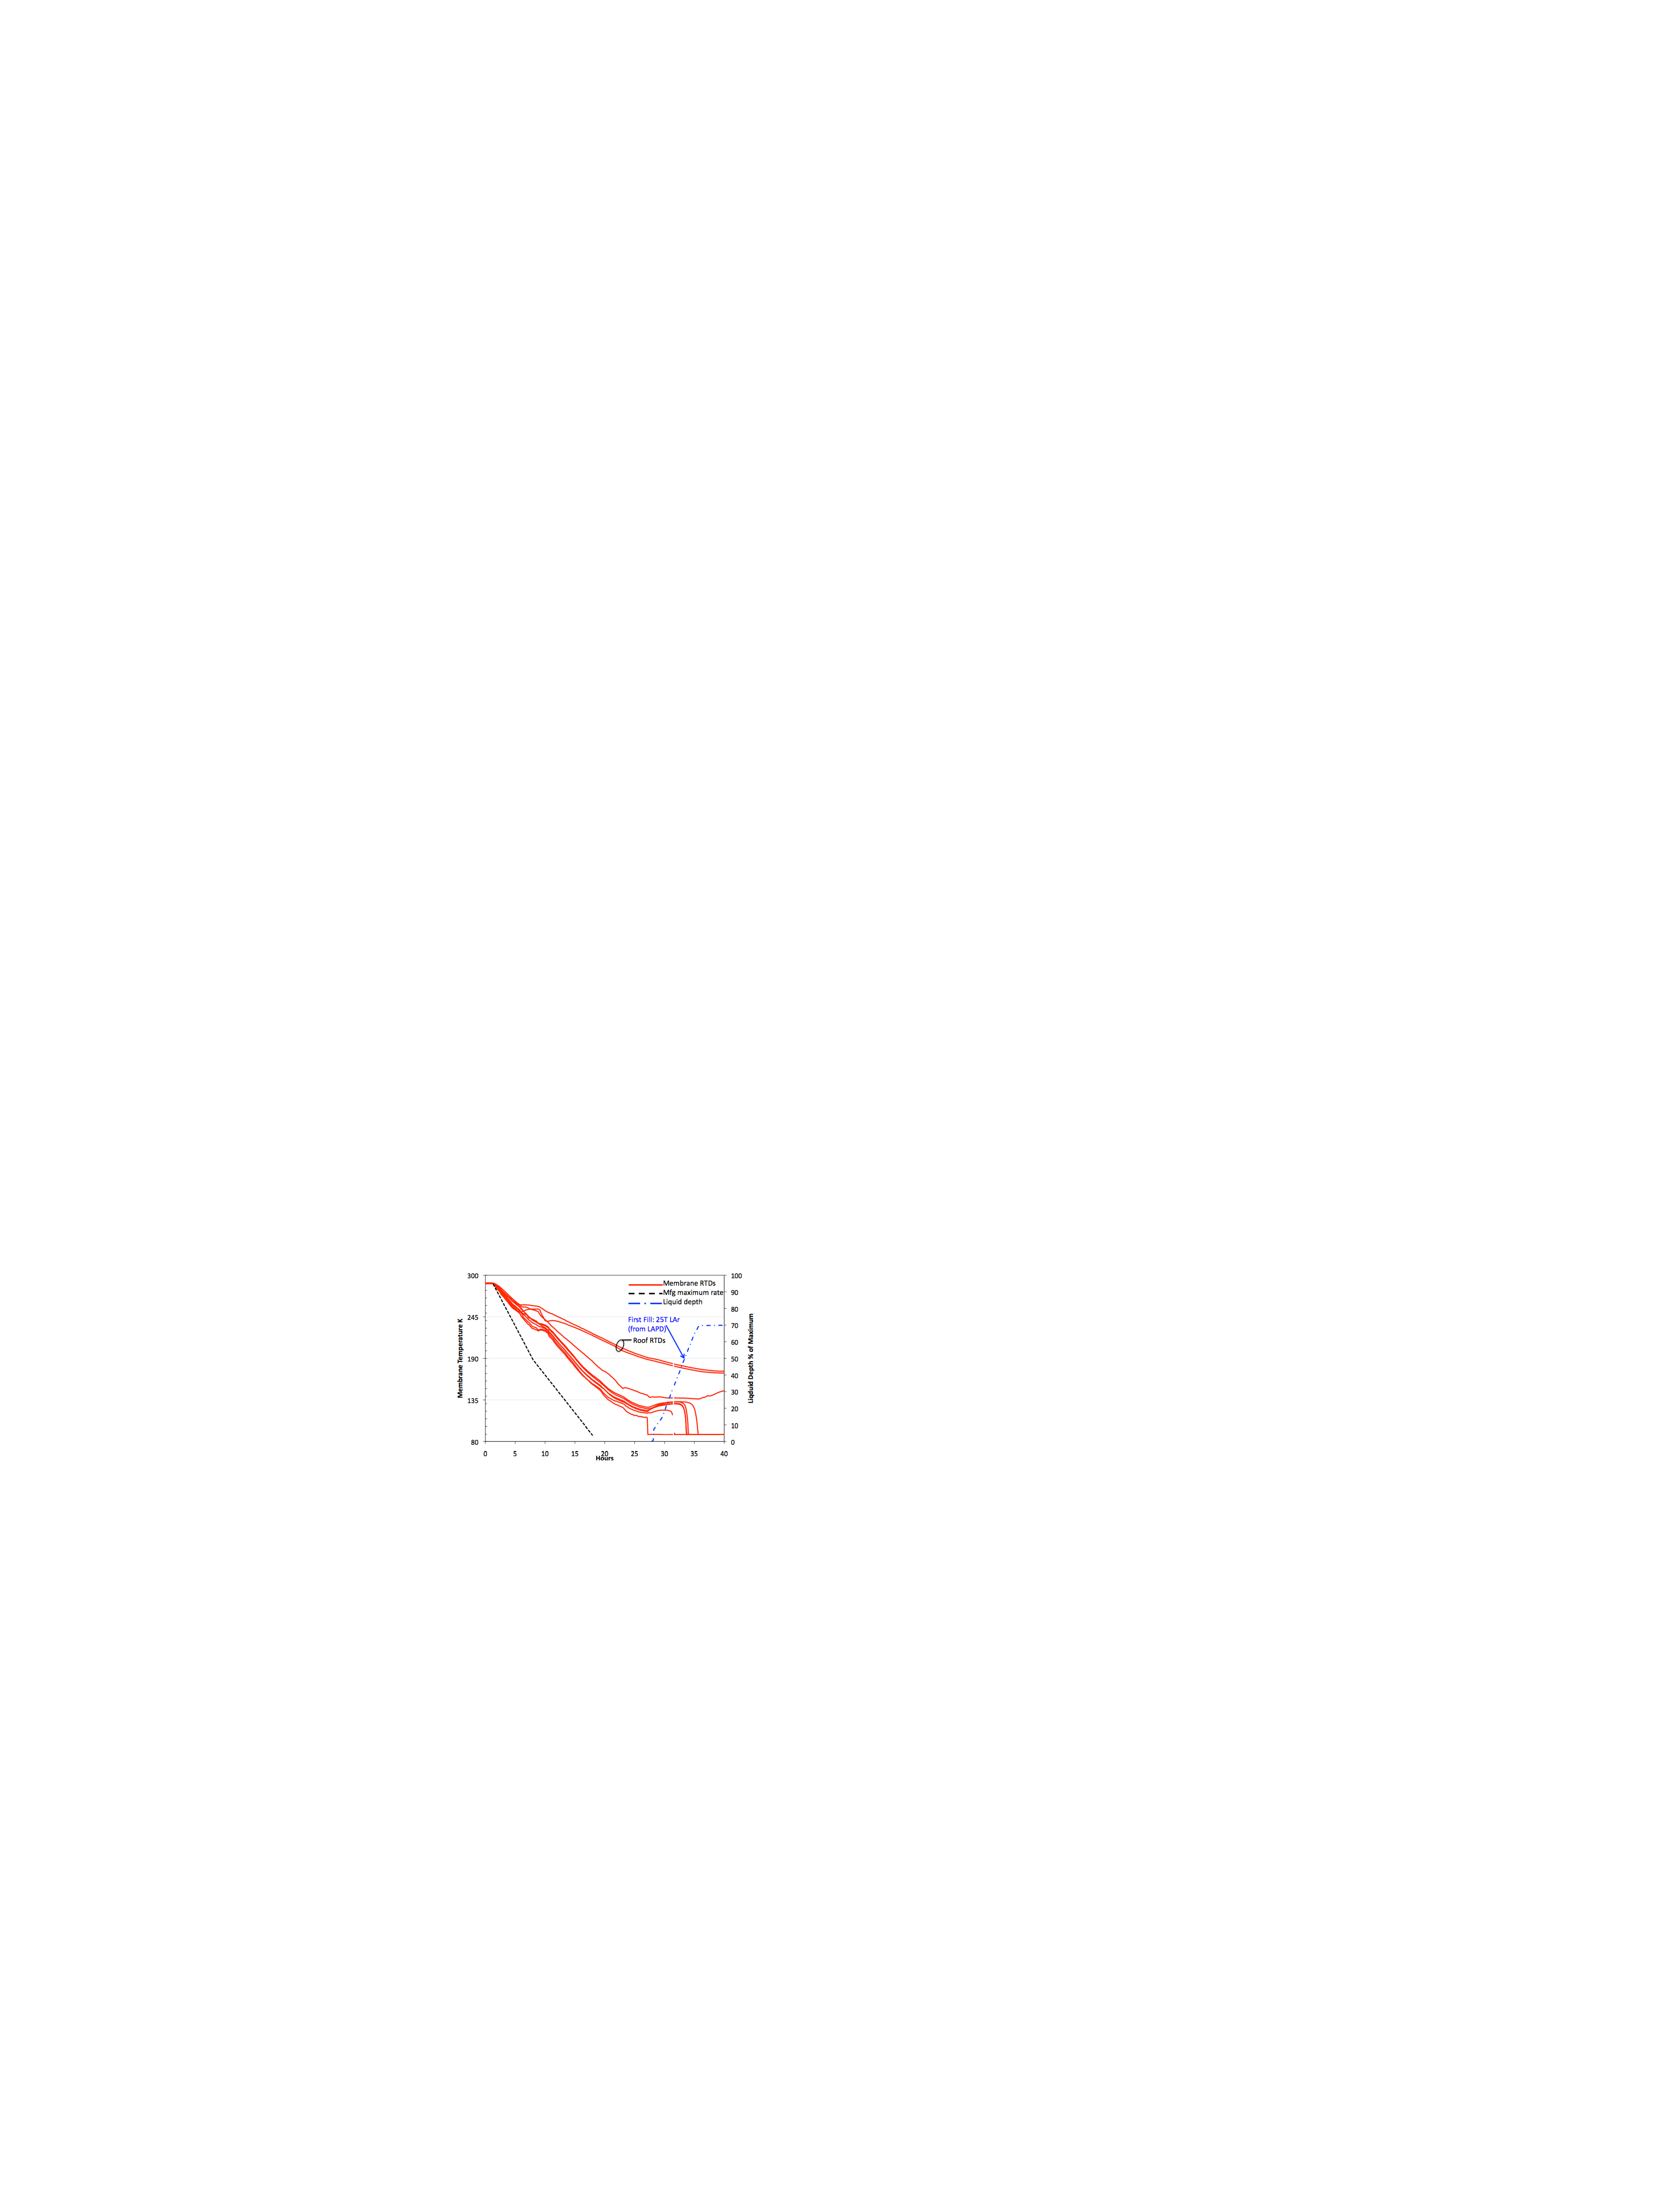
\includegraphics[width=0.98\textwidth]{35tonLiquidFilling.pdf}
    \caption{Liquid filling.}
    \label{fig:35tonLiquidFilling}
  \end{subfigure}
  \caption[Filling the 35-ton cryostat in four stages: piston purge, gas recirculation, cooldown and liquid filling.]{Filling the 35-ton cryostat in four stages: piston purge, gas recirculation, cooldown, liquid filling \cite{35tonPhaseI2015}.  The gas filling is shown in Figure~\ref{fig:35tonGasFilling} and involves using a piston purge to fill the tank with warm gaseous argon before circulating this gas through the filtration system.  Cooldown and liquid filling is demonstrated in Figure~\ref{fig:35tonLiquidFilling}, which shows the falling temperature of the cryostat, as a result of the injection of liquid argon through the cooldown sprayers, and the rising LAr level as the cryostat is filled from LAPD.  The red lines represent temperature measured by various sensors, with the relevant scale on the left, and the liquid depth is shown by the dashed blue line and quantified by the right axis.}
  \label{fig:35tonFilling}
\end{figure}

%----------------------------------------------------------------------------------------------------------------------------------------------------------------------------
\subsection{Outcomes of Phase~I}\label{sec:35tonPhaseIOutcomes}

The 35-ton Phase~I successfully demonstrated the feasibility of membrane cryostats for use with LAr and additionally showed the required LAr purity for future multi-kton LArTPC experiments may be achieved and held in such a vessel.  The lifetime over the course of the $\sim2$~month run, along with external changes to the system, is comprehensively summarised in Figure~\ref{fig:35tonPhaseIElectronLifetime}.

\begin{figure}
  \centering
  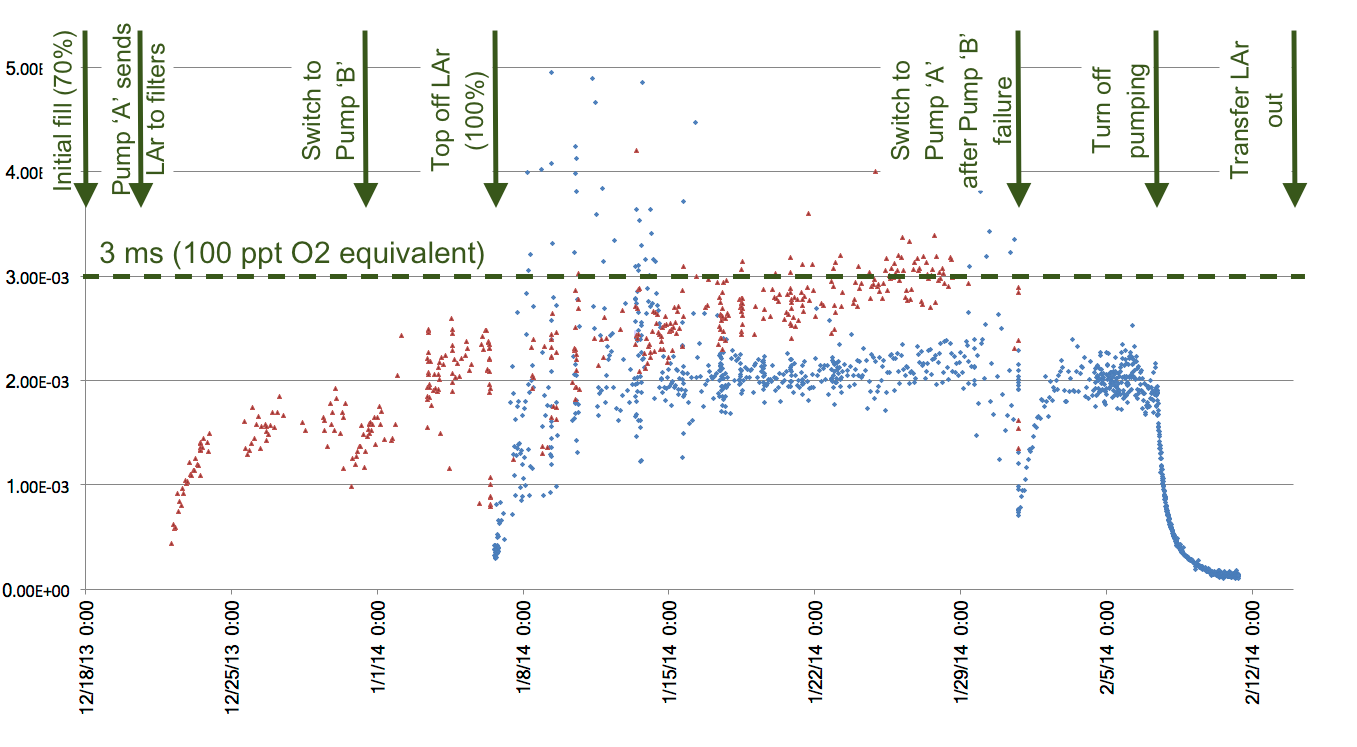
\includegraphics[width=12cm]{35tonPhaseIElectronLifetimeEdit.png}
%  \caption[The electron lifetime in the 35-ton cryostat measured by two purity monitors over the course of the two month Phase~I run.]{The electron lifetime in the 35-ton cryostat measured by two purity monitors over the course of the two month Phase~I run \cite{35tonPhaseI2014}.  The measurements correspond to different positions in the cryostat, with the red points showing purity measurements at the bottom and blue points near the top.  Major external factors affecting the observed LAr purity are shown at the top of the figure.  The old LBNE requirement of 1.4~ms is noted as a dashed grey line; DUNE now requires 3~ms lifetime, equivalent to 100~ppt O$_2$ and illustrated by the black dashed line.}
  \caption[The electron lifetime in the 35-ton cryostat measured by two purity monitors over the course of the two month Phase~I run.]{The electron lifetime in the 35-ton cryostat measured by two purity monitors over the course of the two month Phase~I run \cite{35tonPhaseI2014}.  The measurements correspond to different positions in the cryostat, with the red points showing purity measurements at the bottom and blue points near the top.  Major external factors affecting the observed LAr purity are shown at the top of the figure.  The DUNE requirement of 3~ms lifetime, equivalent to 100~ppt O$_2$, is illustrated by the dashed line.}
  \label{fig:35tonPhaseIElectronLifetime}
\end{figure}

The observed lifetime reached the DUNE requirement and was maintained for a significant period of time; this is a major achievement in the context of the future of LArTPC experiments.  Dips in the purity were observed when topping up the cryostat after initially filling one LAPD volume, and when switching between the two pumps installed to extract the liquid for purification.  In both cases, good purity is recovered after a few volume exchanges.

The same variations of lifetime on temperature were observed as previously noticed in the MTS and LAPD, suggesting a genuine effect dependent on the ambient conditions.  Additionally, during gas circulation, a leak was found and fixed in a seal and, during cold operations, a leak developed in the argon cryo-piping as the dielectric breaks necessary to electrically isolate the cryostat from the building were not leak tight at cryogenic temperatures.  All associated 35-ton experience is useful as progress continues to larger and more complicated LAr cryostats.

The success of the 35-ton was exploited by utilising the existing setup for a second run, involving a small-scale DUNE-style detector.  This would be the first time a membrane cryostat would facilitate a detector and is the next stage along in prototyping the DUNE far detector.

%----------------------------------------------------------------------------------------------------------------------------------------------------------------------------
\section{35-ton Experiment: Phase~II}\label{sec:35tonPhaseII}

The first (and to date, only) particle detector housed within a membrane cryostat was the 35-ton Phase~II.  Following the positive outcomes of the 35-ton Phase~I (discussed in Section~\ref{sec:35tonPhaseI}), it is natural to extend operations to include a prototype DUNE detector.  The initial aims of the 35-ton Phase~II experiment were to develop, build and install a working TPC within the existing cryostat and infrastructure and make measurements of particle interactions induced by cosmic muons whilst demonstrating the required LAr purity is still maintained within a integrated system.  The far detector design was heavily constrained by construction, transport, assembly, time and cost requirements, and prototyping is essential to demonstrate the required spatial, time and energy resolution, signal-to-noise performance, detection efficiency and uptime may be achieved.

The operation of the second 35-ton phase will be discussed in detail in this section.  An overview of the detector is provided in Section~\ref{sec:35tonDetector} before the data acquisition from the detector elements is discussed in Section~\ref{sec:35tonDataAcquisition}.  The custom camera system developed at Sheffield for detecting dielectric breakdown of the LAr is the subject of Section~\ref{sec:SheffieldCameras}.  Finally, the period of data taking is outlined in Section~\ref{sec:35tonPhaseIIRun} before outcomes of the project are presented in Section~\ref{sec:35tonPhaseIIOutcomes}.

%----------------------------------------------------------------------------------------------------------------------------------------------------------------------------
\subsection{The 35-ton Detector}\label{sec:35tonDetector}

A cutaway view of the 35-ton cryostat showing the detector installed is shown in Figure~\ref{fig:35tonDetector}.  The detector elements are designed to prototype as many features of the DUNE far detector (shown in Figure~\ref{fig:DUNEFarDetectorDesign}) as possible.  The readout is performed by four APAs with wrapped induction wires and cold front end electronics (amplifiers and digitisers), which read out multiple drift regions simultaneously.  Embedded within the APAs are photon detectors, representing three different design choices, to trigger on scintillation light.  The drift field is enabled by cathodes at either end of the TPC.  A flange placed on Plate A (referring back to Figure~\ref{fig:35tonCryostat}) facilitates a warm/cold interface through which all electrical signals and the high voltage (HV) feedthrough pass.  Surrounding the walls of the cryostat are over 100 scintillation paddles (Cosmic Ray Counters, CRCs) to provide additional triggers from through-going cosmic muons.

\begin{figure}
  \centering
  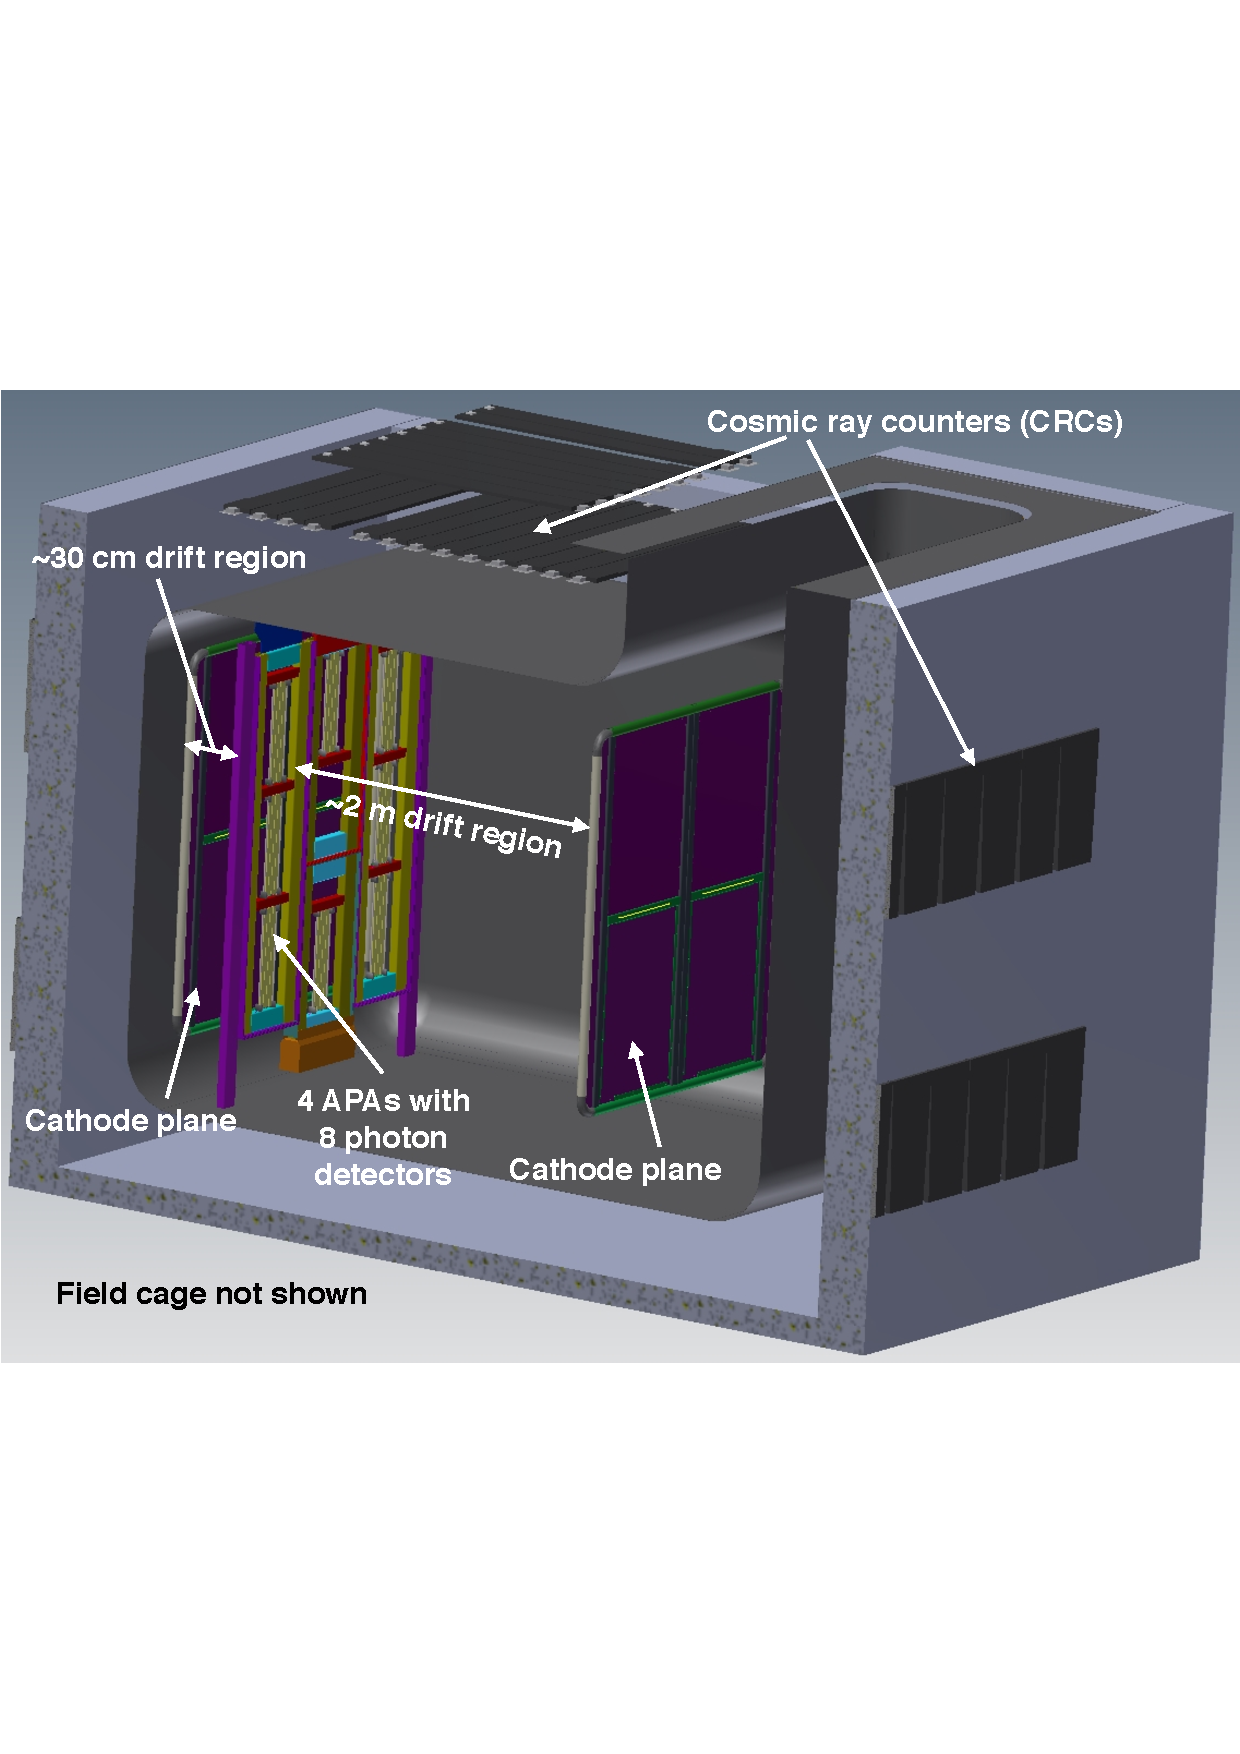
\includegraphics[width=10cm]{35tonDetector.pdf}
  \caption[The 35-ton detector operated during Phase~II of the 35-ton programme.]{The 35-ton detector operated during Phase~II of the 35-ton program \cite{35tonPhaseINeutrino2014}.}
  \label{fig:35tonDetector}
\end{figure}

The three main detector components, the TPC, photon detection system (PDS) and CRCs, are discussed in the following sections.  A photograph of the partially installed detector is shown in Figure~\ref{fig:35tonPhoto} highlighting most of the detector during construction.

\begin{figure}
  \centering
  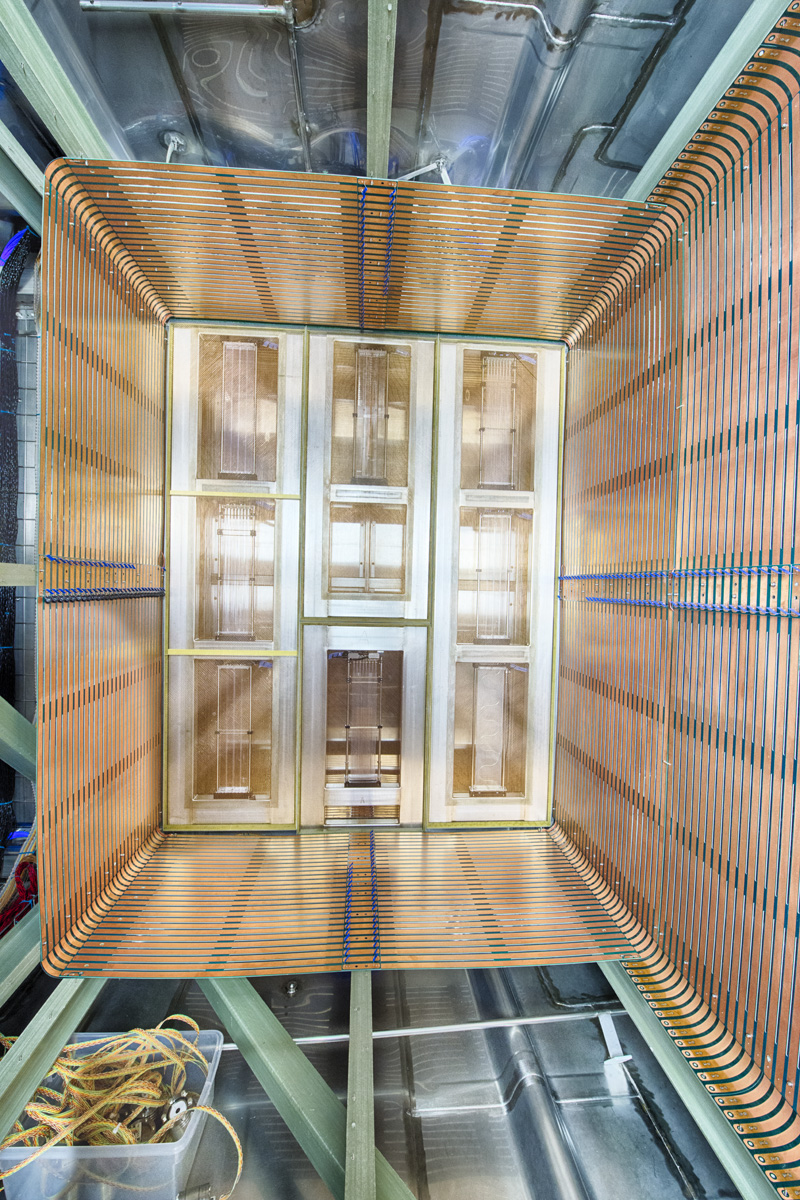
\includegraphics[width=11cm]{35tonPhoto.jpg}
  \caption[Photograph of the partially installed 35-ton detector.]{Photograph of the partially installed 35-ton detector \cite{VMS}.  The four APAs, with the embedded photon detectors, are visible and the field cage is under construction.  Cameras and cold cabling from the Sheffield Camera System, the subject of Section~\ref{sec:SheffieldCameras}, may be observed in a box, prior to installation, at the bottom of the photo.}
  \label{fig:35tonPhoto}
\end{figure}

%----------------------------------------------------------------------------------------------------------------------------------------------------------------------------
\subsubsection{TPC}\label{sec:35tonTPC}

The 35-ton TPC is very similar to the DUNE single phase design introduced in Section~\ref{sec:DUNESinglePhase}.  It has a modular form, with multiple APAs reading out separate drift volumes, and two drift regions: the `long drift region' of length 2.26~m and the `short drift region', around 0.30~m long.  These were chosen to ensure the longest possible drift region in order to closely resemble the far detector drift distances, whilst ensuring the double-sided readout of the APAs may be tested.  Four APAs are used with a very similar design to that depicted in Figure~\ref{fig:DUNEFarDetectorAPA}; each contains two wrapped induction views with a grid and collection plane on each face.  The main difference between the APAs tested in the 35-ton and the current DUNE far detector design is the dimensions of the frames and the angle of the induction wires.  There are three sizes of 35-ton APA; two tall (204~(height)~$\times$~52~(width)~cm) either side of two shorter structures stacked vertically (upper APA dimensions 112~(height)~$\times$~52~(width)~cm and lower APA dimensions 92~(height)~$\times$~52~(width)~cm).  The induction wires are wrapped at an angle of around 45$^{\circ}$, as opposed to 37$^{\circ}$, with slight differences between the planes to ensure the degeneracy is broken (angles of 45.7$^{\circ}$ and 44.3$^{\circ}$ are used).  The angle of 45$^{\circ}$ was initially chosen to optimise the physics reach by providing a high degree of spatial resolution for reconstruction of deposited charge but, following studies of the pattern-recognition performance, and experience with the 35-ton, the angles in the current design were chosen to facilitate a more straight forward disambiguation.

With four APAs and two separate drift regions, there are eight independent drift volumes (DVs), often also referred to as TPCs.  These are demonstrated as part of the geometry in Figure~\ref{fig:35tonGeometry}.  The coordinate system is defined in this figure; the drift direction is described by the $x$-coordinate, and the dimension across an APA face, along which the collection planes are spaced, uses the $z$-coordinate (explaining the denotation of this plane as the Z plane).  The $y$-coordinate is parallel to the orientation of the vertical wires.  The origin is at the edge of one of the long APAs and is such that $x=0$ is at the centre of the APA frames with positive $x$ pointing into the long drift region, $y=0$ is half way between the two short centre APAs and $z=0$ is at the right hand side of the APAs when looking from the long drift region with positive $z$ directed across the faces of the APAs.

\begin{figure}
  \centering
  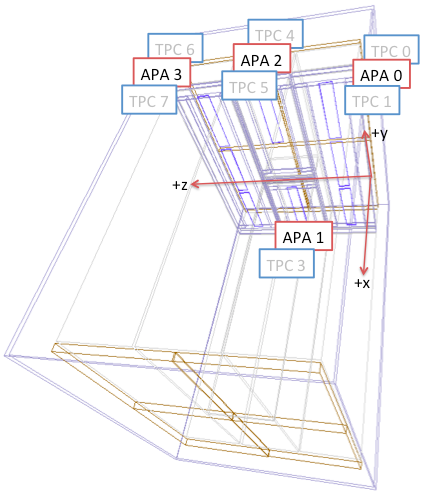
\includegraphics[width=8cm]{35tonGeometry.png}
  \caption[The 35-ton TPC geometry.]{The 35-ton TPC geometry and coordinate system \cite{35tonGeometryAlion2014}.  The blue frames represent the APAs and the orange the CPAs.  The eight separate drift volumes resulting from the modular TPC form are labelled TPC0--7.}
  \label{fig:35tonGeometry}
\end{figure}

The cathode and HV feedthroughs are designed to facilitate a voltage of 120~kV, providing the nominal field of 500~V/cm.  A field cage constructed using FR4 printed circuit board surrounds the open sides of the TPC to establish the necessary electric field.  This was the old LBNE design and has since evolved in the current DUNE outlook; it still enabled a study of the required field within a LArTPC however.

The TPC readout is similar to the DUNE design, with cold preamplifiers, signal shaping and digitisation implemented in ASICs mounted on front end boards at the ends of the APAs.  This is the first time a fully cold signal readout has been implemented in a LArTPC experiment and will be discussed in more detail in Section~\ref{sec:35tonElectronicsReadout}.

%----------------------------------------------------------------------------------------------------------------------------------------------------------------------------
\subsubsection{Photon Detectors}\label{sec:35tonPhotonDetectors}

Three designs of photon detector were utilised in the 35-ton, none of which are current far detector considerations.  These were implemented within APAs in between the wire planes as eight separate units, demonstrated in Figure~\ref{fig:35tonPhotonDetectors} \cite{35tonPhotonDetectors}.  In the figure, the green detectors are the most similar to the current DUNE design and consist of a plastic bar with wavelength shifter (WLS); the blue and red detectors utilise designs of bundled fibres and plates embedded with WLS fibres respectively.

\begin{figure}
  \centering
  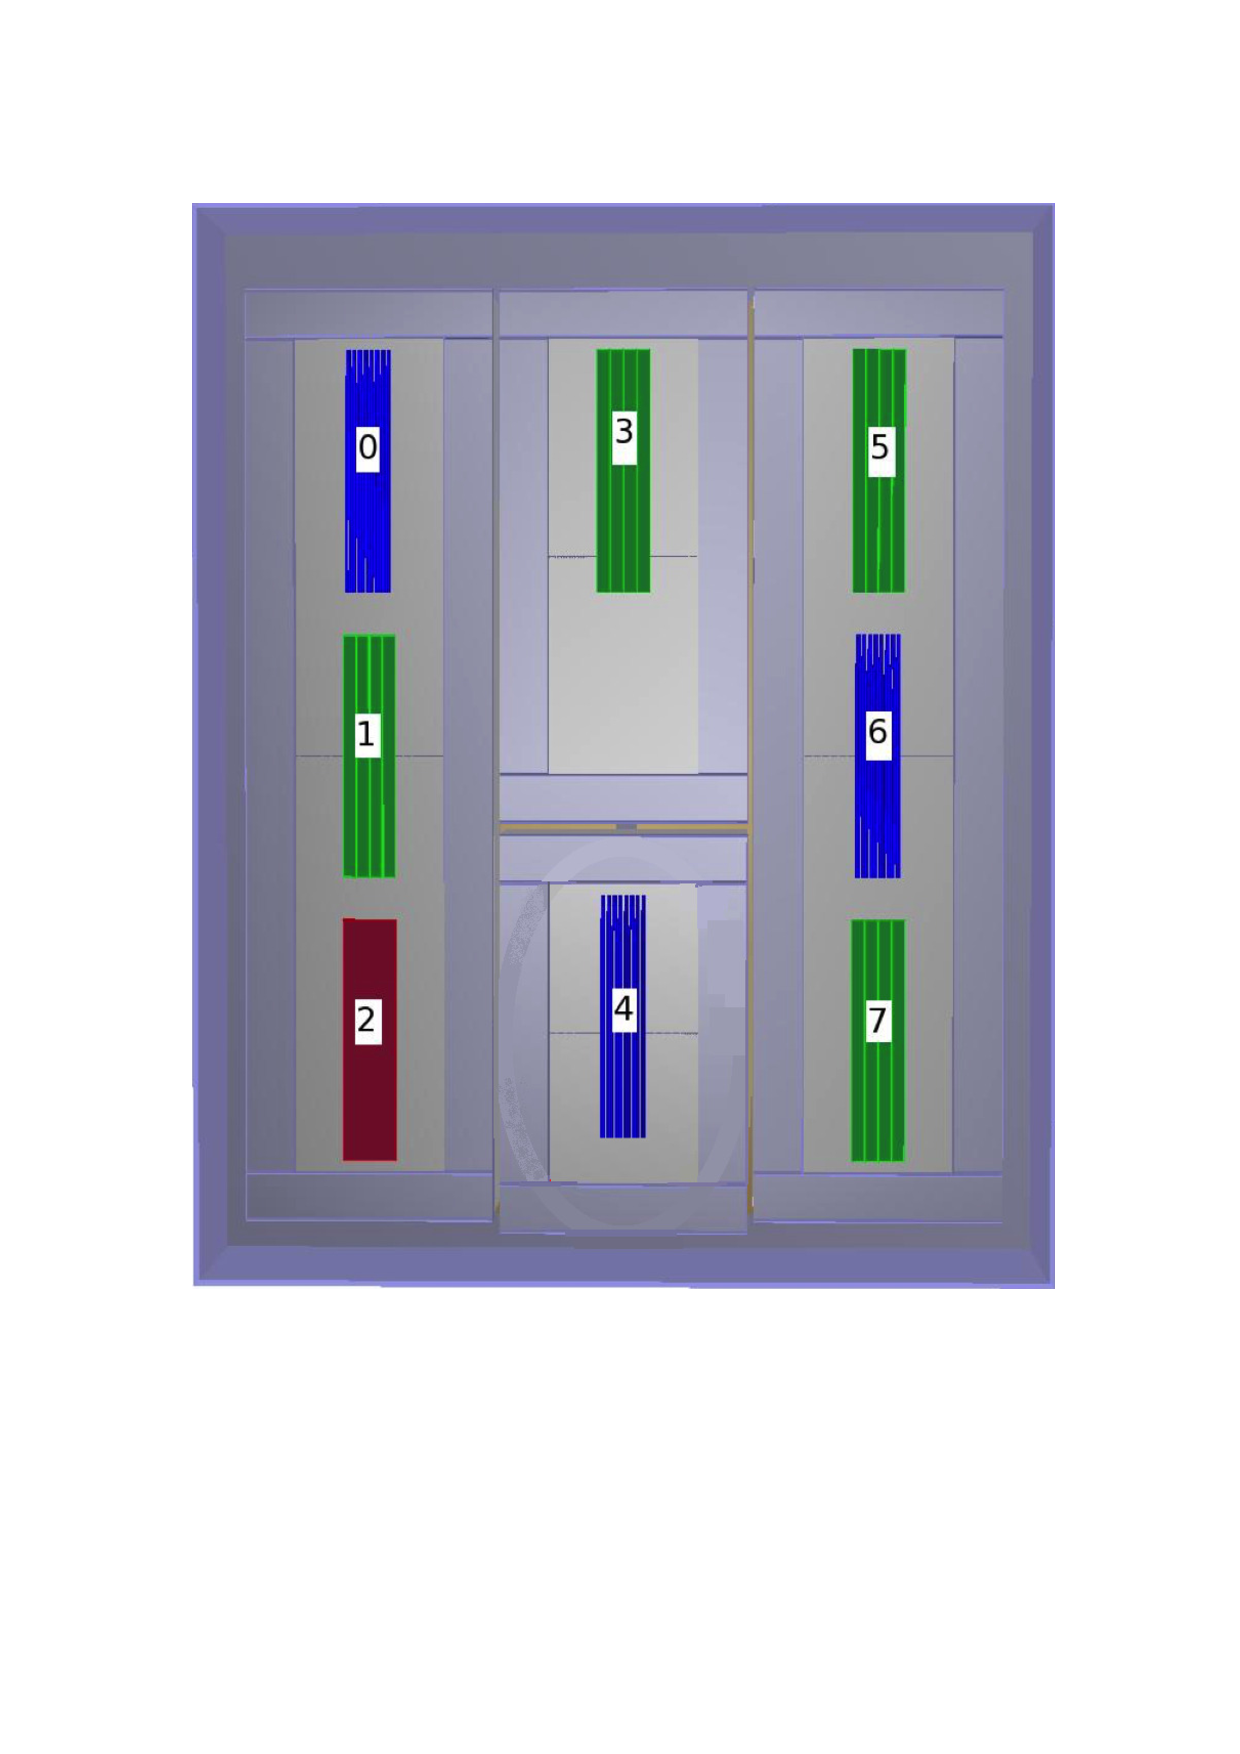
\includegraphics[width=6cm]{35tonPhotonDetectors.pdf}
  \caption[Photon detector units as implemented within the 35-ton APAs.]{Photon detector units as implemented within the 35-ton APAs \cite{35tonPhotonDetectors}.}
  \label{fig:35tonPhotonDetectors}
\end{figure}

All detectors were read out by SiPMs which send analogue signals outside the cryostat, via optical cables, for processing.  It was following experiences from the 35-ton that the DUNE far detector design evolved (shown in Figure~\ref{fig:DUNEPhotonDetectors}).  In the current plan, the detectors are orthogonal to the 35-ton versions and are inserted after the wire wrapping.

%----------------------------------------------------------------------------------------------------------------------------------------------------------------------------
\subsubsection{External Counters}\label{sec:35tonExternalCounters}

In order to provide an additional external trigger system, the 35-ton detector is instrumented with CRCs repurposed from the CDF muon upgrade detectors \cite{CDFCounters2005}.  Most are located on the outer walls of the cryostat, around all four sides and on top of Plate~B on the roof.  There are additional counters in the ceiling of the building directly above the 35-ton cryostat.  The positioning of all the scintillator paddles is shown in Figure~\ref{fig:35tonExternalCounters}.  There are two separate triggers provided by the counters: the `telescope trigger' caused by coincident hits recorded by the counters in the ceiling and those on the cryostat roof, and the `horizontal trigger' caused by coincident counter hits on opposite walls of the cryostat (further subcategorised into `EW' and `NS' triggers).  The trigger rate for telescope muons is on the order of 60~Hz whilst horizontal muons trigger at a rate of around 2-3~Hz.

\begin{figure}
  \centering
  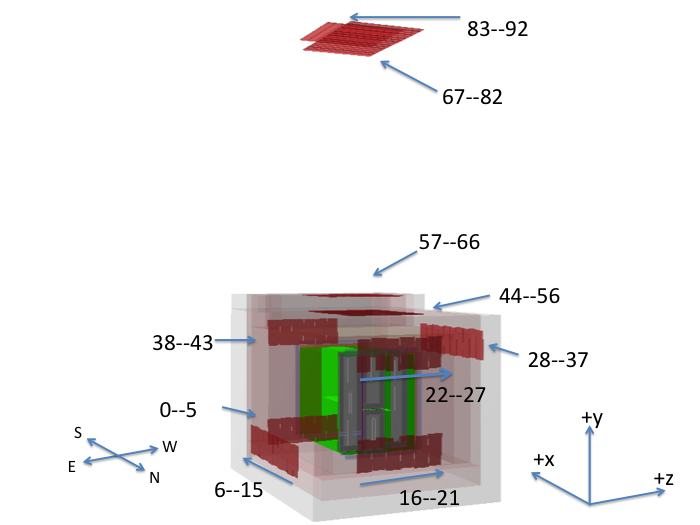
\includegraphics[width=12cm]{35tonExternalCounters.png}
  \caption[The location of the external counters positioned around the outer walls and in the ceiling above the 35-ton cryostat.]{The location of the external counters positioned around the outer walls and in the ceiling above the 35-ton cryostat \cite{35tonExternalCounters}.}
  \label{fig:35tonExternalCounters}
\end{figure}

%----------------------------------------------------------------------------------------------------------------------------------------------------------------------------
\subsection{Data Acquisition}\label{sec:35tonDataAcquisition}

The process of reading out the data from charge deposits on the anode planes through to the resulting data file on disk which may be utilised for subsequent analysis is the subject of this section.  The hardware components, including all readout electronics and processing units, will be briefly described in Section~\ref{sec:35tonElectronicsReadout}.  The data formats produced by the readout components are the subject of Section~\ref{sec:35tonDataFormats} before the software composing the data acquisition (DAQ) system is overviewed in Section~\ref{sec:35tonDAQ}.

%----------------------------------------------------------------------------------------------------------------------------------------------------------------------------
\subsubsection{Electronics and Readout}\label{sec:35tonElectronicsReadout}

The Front End Mother Boards (FEMBs) mounted on the end of the APAs contain two ASICs \cite{DeGeronimo2011,Thorn2012}; the `front end ASIC', which provides signal time-shaping at either 0.5~$\mu$s, 1.0~$\mu$s, 2.0~$\mu$s or 3.0~$\mu$s and amplification at gain settings of either 4.7~mV/fC, 7.8~mV/fC, 14~mV/fC or 25~mV/fC; and the `ADC ASIC' (Analogue-Digital-Conversion) to perform 12-bit digitisation.  A configuration of 3~$\mu$s, 14~mV/fC was selected for normal data taking in order to maximise the signal/noise ratio in the collected data.  The digitised signals are extracted by Reconfigurable Computing Elements (RCEs) \cite{Herbst2014}, developed at SLAC, which trigger, buffer and format the data and send it downstream to the DAQ framework.  The digitising rate is 2~MHz, with the unit of time corresponding to an ADC sample described as a `tick' and equal to 500~ns.

%% \begin{figure}
%%   \centering
%%   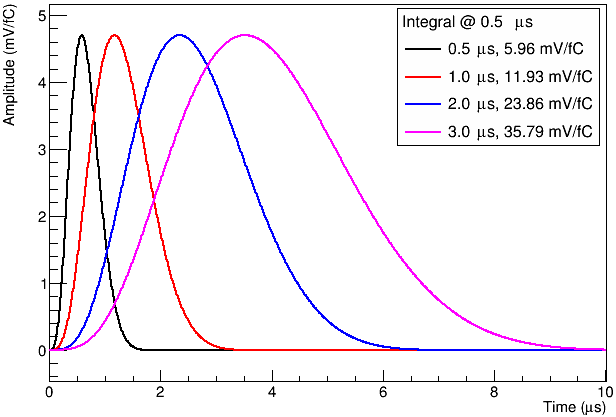
\includegraphics[width=10cm]{ElectronicsResponse.png}
%%   \caption[Electronics response of the front end ASIC for different configuration settings.]{Electronics response of the front end ASIC for different configuration settings. {\color{red} Do I need this?}}
%%   \label{fig:ElectronicsResponse}
%% \end{figure}

The photon detector information is digitised outside the cryostat by custom built units named `SiPM Signal Processors' (SSPs) \cite{SSPManual2016}, built at Argonne National Lab.  Each SSP reads out 12 channels and contains a fully differential voltage amplifier and a 14-bit ADC for signal digitisation.  Along with the RCE output, the SSPs transmit the processed signals to separate computers running the DAQ software.

The triggers are handled by the Penn Trigger Board (PTB), developed at the University of Pennsylvania, which also manages the CRC readout \cite{Barros2016}.  A simplified block diagram of the triggering system is shown in Figure~\ref{fig:35tonTriggering}.  The PTB is designed to receive sub-system triggers (e.g. from the PDS) and generate global triggers, including internal triggers, and timestamps for the whole detector.  It is additionally the front-end for the counter system and handles the reading out of all channels, forming counter `hits' (when a counter has turned on or off) and constructing triggers based on coincidences of these counter hits.  It has a backend which is designed to be compatible with the DAQ system, and sends all information downstream to the acquisition software after the on-board logic has formed the relevant data products.

\begin{figure}
  \centering
  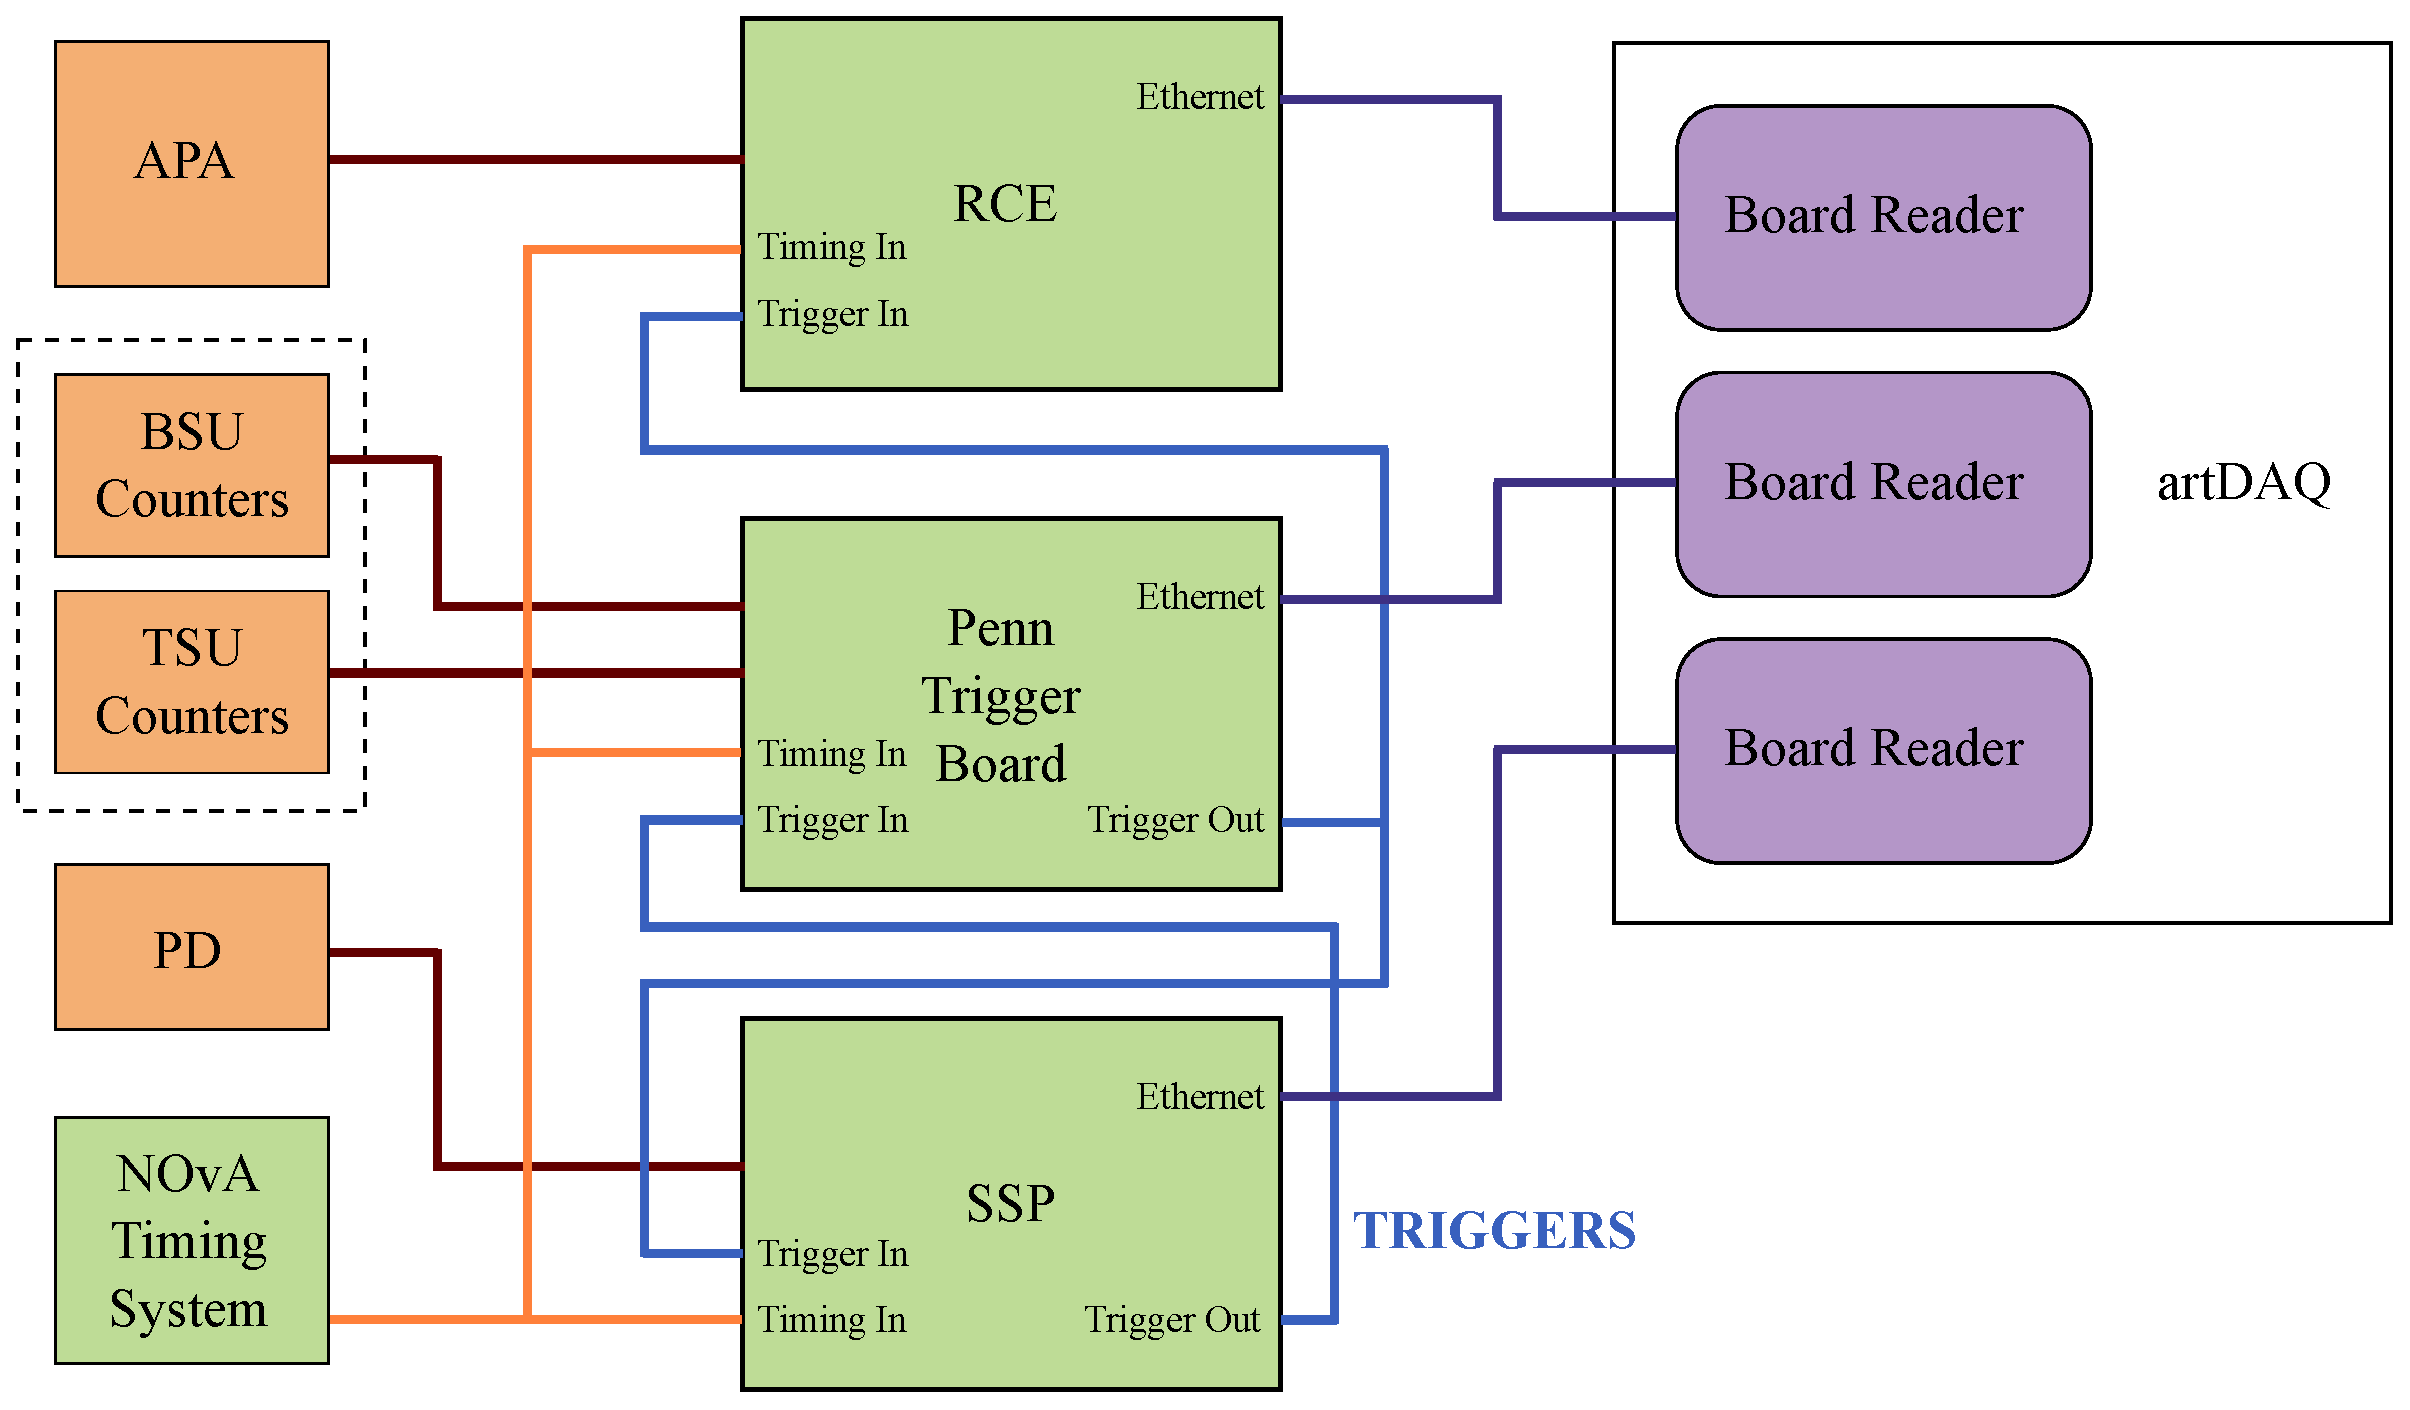
\includegraphics[width=12cm]{trigger_system.eps}
  \caption[Block diagram showing the triggering system for the 35-ton Phase~II.]{Block diagram showing the triggering system for the 35-ton Phase~II.  The Penn Trigger Board handles triggers from the CRCs (labelled as TSU and BSU counters) and also from other detector components, such as the PDS.  Adapted from \cite{Barros2016}.}
  \label{fig:35tonTriggering}
\end{figure}

%----------------------------------------------------------------------------------------------------------------------------------------------------------------------------
\subsubsection{35-ton Data Formats}\label{sec:35tonDataFormats}

The raw data format employs the concept of a `millislice' as a unified data structure common across all detector subcomponents.  An event is a collection of millislices, with one for each of the components being utilised (RCEs, SSPs, PTB).  Each contains substructure unique to the detector element; a simplified overview is provided in Figure~\ref{fig:35tonDataFormat}.

\begin{figure}
  \centering
  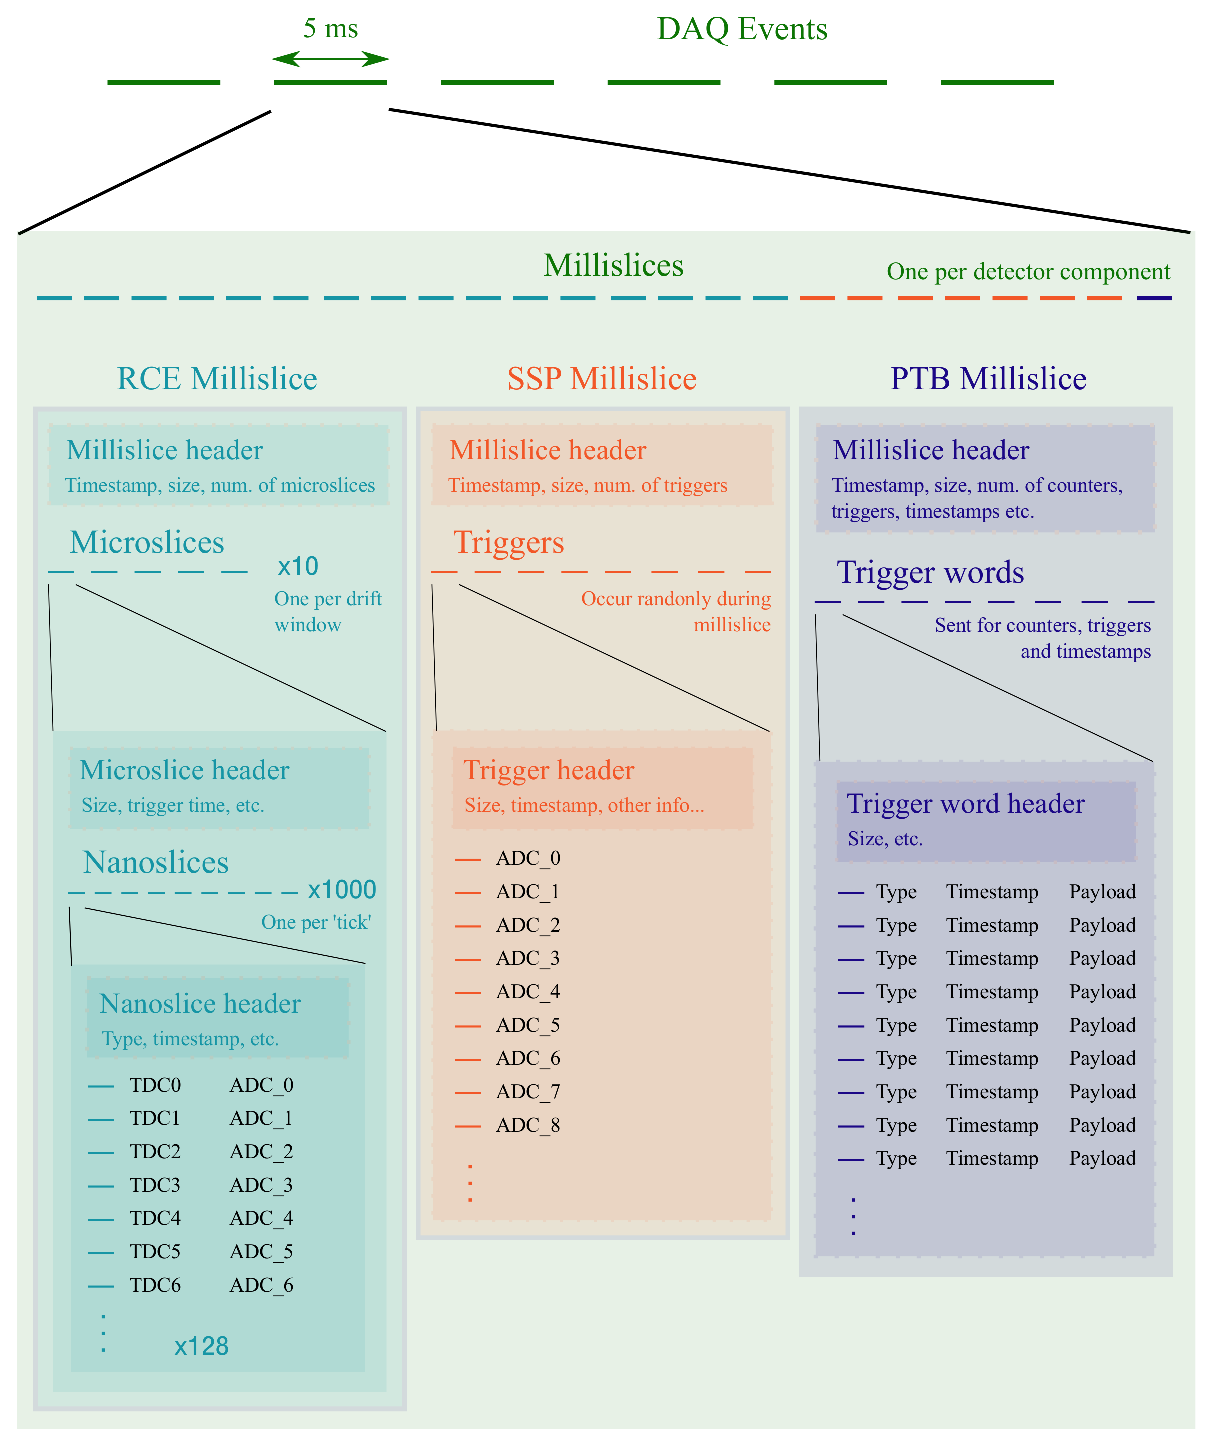
\includegraphics[width=14cm]{data_format.eps}
  \caption[Demonstration of the format used in 35-ton raw data.]{Demonstration of the format used in 35-ton raw data.  A `DAQ event' is composed of a single millislice from each component, each containing further substructure unique to the readout elements.}
  \label{fig:35tonDataFormat}
\end{figure}

The raw format for the TPC data is complicated and has many levels of structure.  The 2048 TPC channels are read out out by 16 FEMBs, each processed by an RCE and represented by a separate millislice.  For the TPC data, a millislice contains all the information for 128 channels.  This data also has further substructure; a millislice is composed of N `microslices', with each microslice containing M `nanoslices'.  A nanoslice contains 128 ADC values, representing one tick worth of data for 1/16th of the detector.  A microslice thus contains this information for a `drift window' (N ticks) and a millislice a collection of M drift windows.  For the normal data running, N was set to 20 and M was 1000.

The data structure output from the SSPs and the PTB is a millislice consisting of a series of triggers filled with relevant information when required.  In the case of the photon detectors, an `SSP trigger' simply describes the waveform for a given channel as a list of ADC values, one for each tick.  A `PTB trigger' is either a counter hit, a trigger or a timestamp and contains a `trigger word' with the type, the timestamp and a variable payload describing relevant further information, such as the channel number or trigger type.  Triggers are created and saved in the SSP and PTB millislices either regularly, when self-triggering, or on the occurrence of an external triggering event, identified by the PDS or the CRCs and handled by the PTB as demonstrated in Figure~\ref{fig:35tonTriggering}.

As data are collected, the RCEs continuously create and save microslices to send to the DAQ to form a millislice.  These microslices are empty (contain no nanoslices) until a trigger is received, at which point nanoslices are made and saved within each microslice.  Additionally, a buffer is in place to save a certain number of full microslices (containing nanoslices) before the microslice containing the trigger.  A certain number of full microslices proceeding the trigger are also recorded by the RCEs.  During normal running, a `$5+1+9$' format was employed; five microslices containing nanoslices before the trigger was received, the microslice containing the trigger, and the nine following microslices.  It should be further noted that, since the DAQ was designed for continuous data readout, these microslices need not necessarily be within the same millislice: it is possible for the trigger to occur in, for example, Microslice~18 of a certain millislice, resulting in the 15 filled microslices straddling successive millislices.  This is demonstrated in Figure~\ref{fig:35tonTriggeredEvent}, and results in real `physics events' being saved in separate `DAQ events'.  To account for this, a splitter/stitcher module has been designed to extract the actual triggered events from the raw data and repackage them into a useful event structure.  This is the first stage before all offline analysis with the 35-ton data.

\begin{figure}
  \centering
  \includegraphics[width=16cm]{triggered_event.eps}
  \caption[Demonstration of how TPC data from a triggered event in a LArTPC is saved when employing a DAQ with continuous readout.]{Demonstration of how TPC data are saved when using a DAQ designed for continuous readout.  The black arrows represent hypothetical triggers occurring within the duration of a particular millislice.  In each case, the five preceding microslices and the nine proceeding microslices are filled with nanoslices and saved; all other microslices are saved with no nanoslices since they contain no useful data.  An example of such an event is shown occurring in Millislice~0 in the figure.  As described in the text, a trigger can cause the useful microslices to straddle consecutive millislices; this is represented in the following millislices in the figure.}
  \label{fig:35tonTriggeredEvent}
\end{figure}

%----------------------------------------------------------------------------------------------------------------------------------------------------------------------------
\subsubsection{35-ton DAQ}\label{sec:35tonDAQ}

Experiments at FNAL are migrating to \textit{artdaq} \cite{Biery2013}, a centrally-maintained data acquisition system built on the \textit{art} \cite{artWebsite,art2012} framework utilised by all offline software written for experiments hosted at the lab.  The DUNE 35-ton experiment was one of the first to use this new software (only LArIAT had previously used it for data taking), and utilised an experiment specific system named \textit{lbne-artdaq}.

\begin{figure}
\centering
  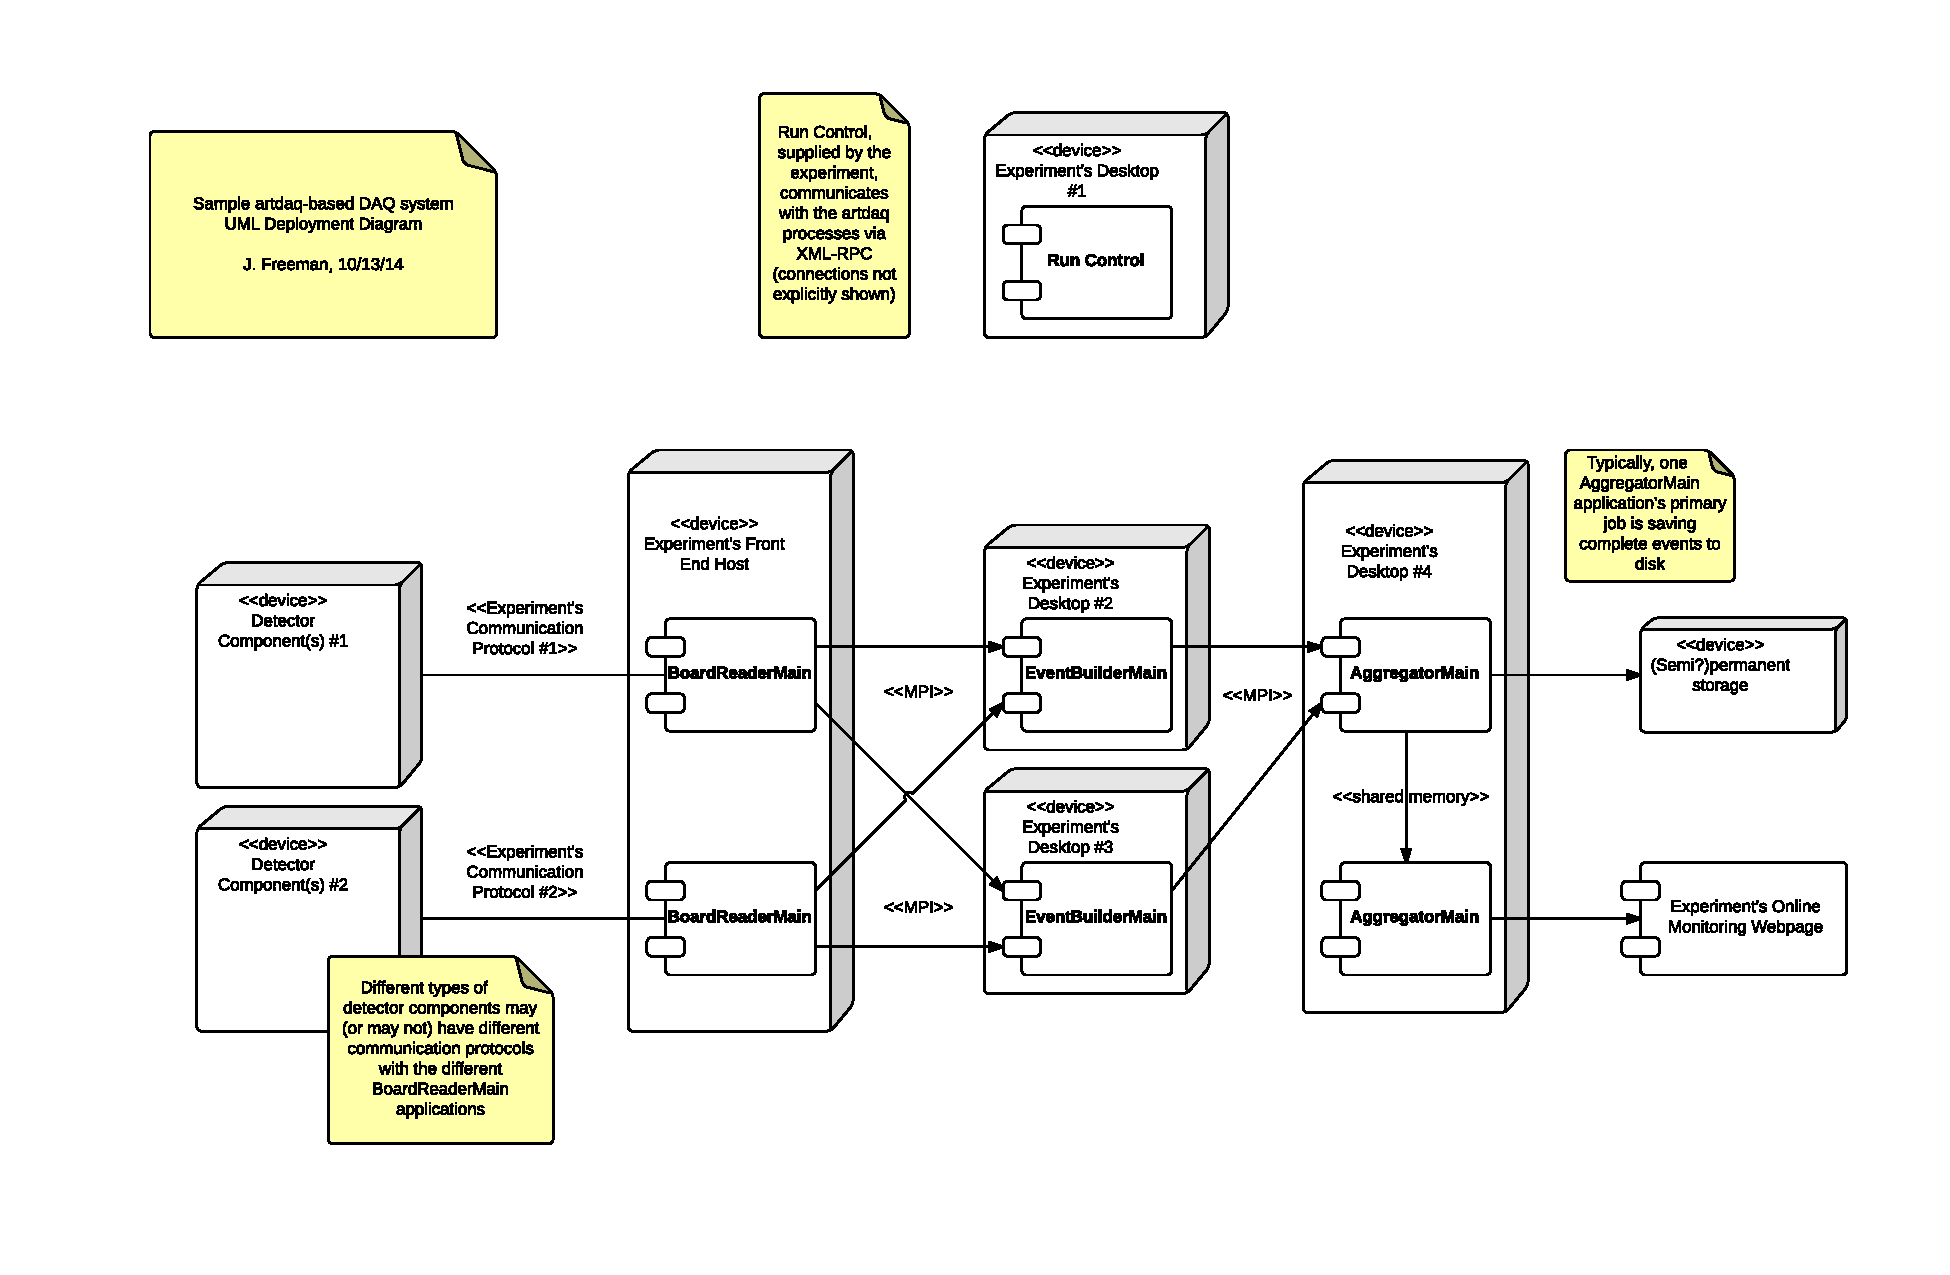
\includegraphics[width=16cm]{artdaqFramework.pdf}
  \caption[Overview of the \textit{lbne-artdaq} framework used for data acquisition by the DUNE 35-ton experiment.]{Overview of the \textit{lbne-artdaq} framework used for data acquisition by the DUNE 35-ton experiment \cite{Freeman2014}.  The detector components are shown on the left before the board readers, event builders and aggregators.}
  \label{fig:lbne-artdaq}
\end{figure}

A general overview of \textit{lbne-artdaq} is shown in Figure~\ref{fig:lbne-artdaq}.  Data flow from left to right and pass through components common to most DAQ systems.  Closest to the detector components (i.e. the RCEs, SSPs and PTB) are the board readers which take the output from the firmware and send it downstream to the event builders.  There exists a board reader for each of the detector components (totalling 24), with each unaware of the existence of the others.  It is the job of the event builders to assemble a full `event' from these individual `fragments' passed on from each of the detector elements.  An event is complete once composed of a full set of fragments and the event builders will wait to receive them all before sending the data onwards to the aggregators.

There are two aggregators which take the full events but process them in very different ways.  All the data passes through the first aggregator, whose function it is to write the output to disk and thus end processing by the DAQ.  The second aggregator receives no events but instead has access to the shared memory occupied by the data as it passes through the first aggregator; it is thus designed specifically for the purpose of monitoring and in no way affects the data or the output from the first aggregator.  This will be discussed further in Chapter~\ref{chap:OnlineMonitoring}.

The 35-ton DAQ was designed to be `triggerless', with the ability to perform continuous readout with a design event rate of 200~Hz.  This is an important feature of the far detector DAQ which is required to ensure data may be recorded safely for non-neutrino beam events, such as nucleon decay or a supernova burst.  This requires high levels of suppression and buffering to ensure rapid movement of data through the system.  In particular, zero suppression for the TPC has been designed such that only ADC values around a window of interest will be kept, vastly reducing the amount of data for the framework to handle.  The DAQ was additionally designed to run in various `modes', such as `scope mode', which focusses on a single channel during running, and `burst mode', designed to collect a sample of data from all channels for a given time upon receiving a trigger.

%----------------------------------------------------------------------------------------------------------------------------------------------------------------------------
\subsection{The Sheffield Camera System}\label{sec:SheffieldCameras}

There are many motivations for developing a camera system which operates at cryogenic temperatures as interest in experiments utilising LAr and LXe (as many dark matter experiments, such as Lux-Zeplin \cite{LZCDR2015}, are considering) progresses.  These include visual monitoring of the cryostat after sealing, including observing the cooldown and filling with cryogenic liquids, and to monitor HV discharge problems.  This latter issue has become cause for concern as LArTPC experiments with very large voltages are being developed; DUNE, for example, will require a cathode HV of $-190$~kV.  Understanding the dielectric properties of LAr is therefore of paramount importance, with recent research suggesting breakdowns occurring at only 40~kV/cm \cite{Blatter2014}.  An additional aim of the 35-ton Phase~II experiment was to study the effects of HV and to search for evidence of HV breakdown of the LAr, which may be used to influence the design of future LArTPC experiments in order to mitigate against these effects.  This is the primary motivation of the camera system deployed in the 35-ton cryostat \cite{35tonCameras2017}, designed at the University of Sheffield and described in this section.

The 35-ton was instrumented with eight cameras; six to monitor high-field locations within the cryostat and for detecting visual sparks from HV breakdowns, and two for diagnosis of different cryogenic systems including the cooldown sprayer and the phase separator.  The fields of view of each of the cameras are demonstrated in the calibration images shown in Figure~\ref{fig:35tonCamerasImages}.

\begin{figure}
  \centering
  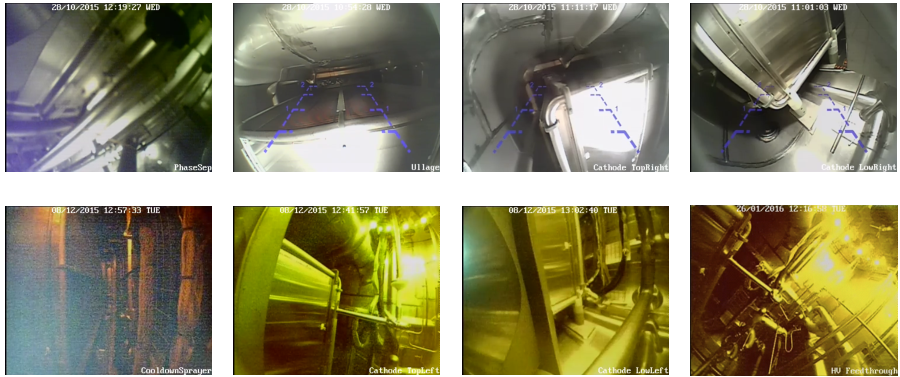
\includegraphics[width=15cm]{35tonCamerasImages.pdf}
  \caption[The calibration images for the 8 cameras in the Sheffield Camera System installed in the 35-ton cryostat.]{The calibration images for the 8 cameras in the Sheffield Camera System installed in the 35-ton cryostat.  Upper (left to right): phase separator, ullage, cathode top right, cathode bottom right.  Lower (left to right) cooldown sprayers, cathode top left, cathode bottom left and high voltage feedthrough.  The upper images were taken with a halogen light illuminating the cryostat, prior to it being sealed up.  The lower images were taken with the LED ring light on, with the cryostat sealed up. All images are left-right inverted due to software.  Taken from \cite{35tonCameras2017}.}
  \label{fig:35tonCamerasImages}
\end{figure}

%----------------------------------------------------------------------------------------------------------------------------------------------------------------------------
\subsubsection{The Camera System}\label{sec:35tonCameraSystem}

Previous cameras designed to study cryogenic liquids have either been placed outside the volume or have been maintained in a heated vessel for protection from the cold surroundings.  A system which operates directly in cryogenic temperatures is desirable when applying the technology to larger-scale cryostats and for possible use in the detection of secondary scintillation light.  Achieving this without an actively heated region in the cryostat is also advantageous to avoid boiling and disturbing the LAr in close proximity.  The camera system developed utilised Complementary Metal-Oxide Semiconductor (CMOS) cameras contained within a module alongside a temperature sensor and small resistive heater.  This is demonstrated in Figure~\ref{fig:35tonCamera}.

\begin{figure}
  \centering
  \begin{subfigure}[t]{0.48\linewidth}
    \centering
    \includegraphics[width=0.98\textwidth]{35tonCameraPhoto.pdf}
    \caption{Photograph.}
    \label{fig:35tonCameraPhoto}
  \end{subfigure}
  \hfill
  \begin{subfigure}[t]{0.48\linewidth}
    \centering
    \includegraphics[width=0.98\textwidth]{35tonCameraSchematic.pdf}
    \caption{Schematic.}
    \label{fig:35tonCameraSchematic}
  \end{subfigure}
  \caption[An example camera module developed for the 35-ton Sheffield camera system.]{An example camera module developed for the 35-ton Sheffield camera system, taken from \cite{35tonCameras2017}.  Figure~\ref{fig:35tonCameraPhoto} shows a sealed camera module and the components of such a module.  Figure~\ref{fig:35tonCameraSchematic} demonstrates schematically the composition of a camera module: from left to right a CF40 flange with 9-pin D-sub feedthrough, double sided CF40 flange, PT100 sensor (green wires), camera (red, black and yellow wires), two heating resistors (blue wires) on either side of the camera connected in series, optical viewport on CF40 flange.}
  \label{fig:35tonCamera}
\end{figure}

The cameras are commercially sold as car-reversing cameras and are rated by the manufacturer down to $-40^{\circ}$C (233~K).  A wide range of cameras were tested and those which consistently performed well in tests whilst at cryogenic temperatures (submerged in liquid nitrogen) were selected.  Around half of these were found to reliably endure power cycling when cold (the inconsistency arising from operating the cameras outside of the recommendations) and it was these which were included in the modules used in the 35-ton.  The heating elements were included as a failsafe mechanism in case the cameras developed a requirement of warmer local temperatures to turn on after sustained periods in the cold.

Each camera contains 712~$\times$~486~pixels and has a roller shutter rate of 50~frames per second.  Their resolution at 10~mm was found to be $(2.0\pm0.5)$~mm at room temperature and $(1.5\pm0.5)$~mm at 77~K, with the improvement at lower temperatures due to a higher refractive index of LN$_2$ resulting in the light becoming less diffuse.  The minimum measurable light pulse width the cameras could trigger on, in both the warm and the cold, was observed to be 20~ns.  One notable change when operating the cameras at cryogenic temperatures was the chrominance output of the video signal.  The usual colour signal is observed as monochromatic when in the cold, possibly due to partial failures on the on-board encoding electronics.

Before installation, the response of the cameras to sparks was characterised by applying a HV across a printed circuit board (PCB) in LAr until breakdown was observed.  The discharge was between 40 and 60~ms and the cameras showed localised sparks persisting over multiple frames of exposure.  The trigger system, which relies on a percentage change in the number of different pixels between successive frames, was also able to successfully detect and automatically record on occurrence of the sparks.

%----------------------------------------------------------------------------------------------------------------------------------------------------------------------------
\subsubsection{Operation and Outcomes of 35-ton Camera System}\label{sec:35tonCameraSystemOperation}

The camera modules were mounted on the existing piping from the cryogenic system within the 35-ton.  An example is shown in the photograph in Figure~\ref{fig:35tonCameraMounted}.  Data acquisition, operation and control was performed using a rack-based system containing a power supply, a temperature sensor reader, DAQ and computer control system.  Full details of the entire arrangement and all the interconnects are available in Figure~\ref{fig:35tonCameraDiagram}.

\begin{figure}
  \centering
  \includegraphics[width=8cm]{35tonCameraMounted.pdf}
  \caption[Two camera modules mounted on cryo piping in the 35-ton cryostat.]{Two camera modules mounted on cryo piping in the 35-ton cryostat.  Taken from \cite{35tonCameras2017}.}
  \label{fig:35tonCameraMounted}
\end{figure}

\begin{figure}
  \centering
  \includegraphics[width=12cm]{35tonCameraDiagram.pdf}
  \caption[Full system block diagram for the camera modules in the DUNE 35-ton prototype.]{Full system block diagram for the camera modules in the DUNE 35-ton prototype.  Taken from \cite{35tonCameras2017}.}
  \label{fig:35tonCameraDiagram}
\end{figure}

The cameras were characterised in room temperature following installation and the software trigger tested on the Xe flash light from the purity monitors (described in Section~\ref{sec:PurityMonitoring}).  The system ran continuously throughout the 10~weeks of the 35-ton Phase~II cooldown.  It was heavily utilised during cooldown and filling to monitor the inside of the cryostat and observe the rising liquid level (an excellent video of the LAr when level with one camera module is available at Reference~\cite{35tonCameraVideo}).  The entire system was power cycled successfully three times during TPC debugging and following the FNAL site wide power outage on 4th March 2016.  The downtime ranged from 30~minutes to 9~days, with the cameras turning on without assistance each time.

The picture quality was observed to degrade noticeably over time, demonstrated in Figure~\ref{fig:35tonCamerasDegredation}, with significant variation between different camera modules.  When in darkness, a greater number of saturated or noisy pixels is observed across the cameras and when illuminated by the LED ring, the noise increase is noticeable with a decreased colour depth.  This is likely due to signal transmission length, power cycling and prolonged exposure to the cold.

\begin{figure}
  \centering
  \includegraphics[width=12cm]{35tonCamerasDegredation.pdf}
  \caption[The variation in picture quality degradation in the 35-ton camera system is illustrated by the changes in Camera~1 and Camera~4 over time.]{The variation in picture quality degradation is illustrated by the changes in Camera~1 (upper) and Camera~4 (lower) over time. Left: prior to cooldown, centre: immediately post-cooldown, right: after 10 weeks submerged in LAr.  The field of view changes due to the change in refractive index.  Note that these are full colour images with no post-processing.  Taken from \cite{35tonCameras2017}.}
  \label{fig:35tonCamerasDegredation}
\end{figure}

Two suspected HV breakdowns occurred during normal operations at 60~kV but the system was unoperational as a result of the power outage during both.  Following the end of running, when testing the HV at 135~kV, four breakdowns occurred with three detected and triggered on by the camera system.  However, the location of the spark could not be determined clearly from the recorded video. This could be due to either the spark occurring outside the cryostat or the field of view of the cameras, an insufficient intensity or duration of the flash or the degradation in picture quality being such that the efficiency and sensitivity of the triggering system were compromised.

The camera system was shown to be successful and a useful aid in 35-ton operations.  Despite not showing HV breakdowns clearly, the modules remained operational during the 35-ton Phase~II run and were valuable for monitoring purposes.  They were shown to trigger successfully on a test bench so it seems reasonable to conclude their inability to do so within the LArTPC was solely due to the degradation in picture quality, which must be improved if such a system were to be used in future LAr experiments.

%----------------------------------------------------------------------------------------------------------------------------------------------------------------------------
\subsection{Phase~II Run}\label{sec:35tonPhaseIIRun}

Following a long period of testing the detector components at FNAL, installation of the TPC and field cage was carried out in October 2015.  This was followed by the final parts of the system, such as the long drift region cathode, the purity monitors, HV feedthrough and cameras, in November 2015.  Following the Fermilab readiness clearance, operations began in December 2015.  This involved piston purging both LAPD and the 35-ton, filling LAPD with LAr delivered from the suppliers, cooling down the 35-ton cryostat and finally transferring the liquid argon from LAPD into the 35-ton.  This was completed by the end of January 2016.

The 35-ton Phase~II run officially started on 11th February 2016 upon the final liquid transfer into the cryostat and the starting of the pumps and recirculation of the LAr through the filtration system.  A week later, the HV on the cathode was ramped up to half nominal value: 60~kV, providing a drift field of 250~V/cm.  The intention was to ensure a sufficient amount of collected data was on disk before proceeding with increasing the HV up to the design voltage of 120~kV (500~V/cm) and even up to the maximum of 135~kV.

The start of the run was dedicated to many noise tests; it was immediately clear the noise on the TPC channels was much larger than anticipated even after the testing from the previous summer.  These tests involved studying each of the FEMBs separately and considering effects from other non-TPC detector elements by removing power from all systems in the cryostat before reintroducing components iteratively.  An additional `high noise state' was also identified, corresponding to a very high oscillatory noise level instantaneously appearing on all channels simultaneously and remaining for up to hours at a time.  The noise problems in the 35-ton Phase~II will be discussed in more detail in Section~\ref{sec:35tonPhaseIIOutcomes}.

This commissioning time was also important as the stability of the DAQ was improved.  Near the beginning of data taking, it was uncommon for the DAQ to run for more than a few minutes with even a small subsection of components (RCEs, SSPs, PTB), with issues such as data throughput, disk writing speed and hardware interface issues contributing to a very unstable system.  In the months of installation and commissioning, the DAQ was the subject of much attention and progress on improving the framework progressed in parallel with the final installation, LAr filling and noise hunting.

Following the completion of the designated noise runs and the stabilising of the DAQ, the focus was on collecting as much data as possible before raising the HV, with the plan to run for at least a week at 90~kV and 120~kV respectively.  However, the run was unfortunately cut short in the early hours of the morning of 19th March 2016 when a tube, part of the system which was introducing GAr from LAPD to the 35-ton purification network in order to maintain the LAr level, sheared and facilitated the introduction of air directly into the filters.  Within a few minutes, faster than it would have been possible to respond even if this incident had not occurred at 3~a.m., the filters were saturated and the entire volume of LAr in the 35-ton was poisoned.  The offending pipe break is shown in Figure~\ref{fig:35tonPipeBreak}.  This incident effectively concluded the data collection prematurely and meant the design HV could not be tested in good quality LAr and no data could be taken at nominal drift field.

\begin{figure}
  \centering
  \includegraphics[width=6cm]{35tonPipeBreak.png}
  \caption[The broken pipe, originally part of the framework introducing gaseous argon from LAPD into the 35-ton to maintain LAr levels, which resulted in the poisoning of the whole LAr volume by allowing the introduction of air into the system.]{The broken pipe, originally part of the framework introducing gaseous argon from LAPD into the 35-ton to maintain LAr levels, which resulted in the poisoning of the whole LAr volume by allowing the introduction of air into the system.}
  \label{fig:35tonPipeBreak}
\end{figure}

The run is summarised in Figure~\ref{fig:35tonPhaseIIData}, showing the LAr purity as a function of time and notable incidents.  The bulk of collected data was either side of a site-wide FNAL power outage on 4th March 2016, after which it took a few days to recover the LAr purity.  After recuperating from this incident, an issue with the LN$_2$ values resulted in a cooling failure and the boiling off of a large portion of the LAr in the cryostat.  The pipe break occurred shortly after rectifying this issue.  These issues plagued the final few weeks of data taking, evident from the corresponding LAr purity in the detector.%  The high frequency of these complications within such a short space of time motivated the description of this period of running as the `Bad News Period' on the figure.

\begin{figure}
  \centering
  \includegraphics[width=14cm]{35tonPhaseIIDataEdit.png}
  \caption[The data taking period of the 35-ton Phase~II experiment.]{The data taking period of the 35-ton Phase~II experiment.  The electron lifetime measured by the two long PrMs in the cryostat is shown as a function of time, with the horizontal axis covering the period 11th~February -- 19th~March~2016.  The numbers within the green boxes represent the amount of data taken, in days, with the drift field of 250~V/cm present.  The major incidents which affected the LAr purity are shown on the figure.}
  \label{fig:35tonPhaseIIData}
\end{figure}

Most of the data taken were triggered using the horizontal muon trigger.  In the last week of running, the telescope trigger was deployed, with a large prescaling due to the high rate of cosmic muons, and the PDS was also used to trigger data taking.  Both systems appeared to work as intended but thorough testing proved impossible due to the temporal proximity to the unforeseen termination of run.  Throughout data taking, the DAQ recorded data to disk at a rate of 1~Hz.  Because of the electronics noise and small signal/noise ratio, tests of data taking using zero suppression were unable to be performed.

Overall, the run provided 22 days of high quality (good LAr purity, high stable voltage, stable DAQ) data, albeit with much higher noise than anticipated.  An example electromagnetic shower observed in the data with strong signals in all planes is depicted in Figure~\ref{fig:FamousShower}.  The noise problems have resulted in limitations to the analyses possible with the 35-ton data and focus has shifted to studies utilising datasets unique to the 35-ton.  Some such analyses are the subject of Chapter~\ref{chap:35tonAnalysis}.

\begin{figure}
  \centering
  \includegraphics[width=12cm]{FamousShower.pdf}
  \caption[Event display depicting the charge deposited by an electromagnetic shower during the 35-ton Phase~II run.]{Event display depicting the charge deposited by an electromagnetic shower during the 35-ton Phase~II run.  The three views are, from the top down, the collection plane and the V and U induction planes.  Each shows the wire number on the horizontal axis and time, measured in units of tick ($\equiv$~500~ns) on the vertical axis.  Charge is represented by the colour scale on the $z$-axis.  The shower is clearly visible in all three planes and demonstrates the functionality of the 35-ton detector.}
  \label{fig:FamousShower}
\end{figure}

%----------------------------------------------------------------------------------------------------------------------------------------------------------------------------
\subsection{Outcomes of Phase~II}\label{sec:35tonPhaseIIOutcomes}

The 35-ton Phase~II collaboration successfully designed, constructed, installed and ran a small-scale DUNE-style LArTPC and collected data whilst maintaining a good LAr purity, with electron lifetimes consistently reported above the DUNE requirement of 3~ms.  This is the first time a detector has been operated within a membrane cryostat and the integrated system has been strongly validated.  The complete process has been instructive and a great many lessons have been learned alongside the successes of the project \cite{35tonLessonsLearned}.

This section will review all these outcomes and discuss how the experience will influence the DUNE programme as it progresses towards the first far detector module.  In general the majority of subsystems achieved or superseded expectations and, following the 35-ton Phase~II experience, there is no reason for reservation over ProtoDUNE as rapid development continues to be made.

%----------------------------------------------------------------------------------------------------------------------------------------------------------------------------
\subsubsection{Cryostat and TPC}\label{sec:35tonPhaseIIOutcomesCryostatTPC}

The cryostat and most TPC components behaved as expected and resulted in no unexpected functionality.  When filled with GAr, before the introduction of LAr, the cryostat was leak tested.  When this was performed in Phase~I a few issues were identified and had to be addressed; there were no complications during Phase~II commissioning however.  The pumps were not tested between phases and required a large current to begin their operation with the cryostat already filled with LAr; this demonstrates how vital it is to assess all detector components before commissioning.  Other than the failing in the cooling system, all cryogenics performed excellently.  Since this incident occurred not long after the power outage, the alarm system had not been correctly brought back online, resulting in an avoidably large loss of LAr.  These are two of many examples of lessons learned from the 35-ton.

The HV and drift field presented no issues during the course of the run.  No confirmed breakdowns were observed at 60~kV but testing in clean LAr at 120~kV was not possible.  Although a voltage of 135~kV was attained and held for multiple days in contaminated argon, the impurities are presumed to alter the dielectric properties of the material and therefore complete validation remains unproven.

Results from the purity monitors and temperature sensors suggest a stratification along the height of the LAr volume within the cryostat, similar to observations made during the Phase~I run.  The cause of this is likely due to returning LAr from the purification system being cooled below the `bulk temperature' by the phase separator and reentering near the bottom of the cryostat, resulting in reduced convection and poor mixing.  Resolutions, such as returning warmer LAr to the main volume, are being considered for future LArTPCs in an attempt to mitigate these effects and ensure a good, isotropic purity.

The TPC electronics were the largest source of shortfalls in the experiment and have significantly compromised the utility of the data.  During warm tests over summer 2015, it was evident the intrinsic noise levels in the ASIC electronics were higher than anticipated and an additional issue with the ADC ASIC was observed.  The digitisers are affected by bit-level corruption whereby the six least-significant bits (LSB) or most-significant bits (MSB) are erroneously reported as either 0x0 or 0x3F at a rate, between 20\% and 80\%, which is strongly dependent on the proximity of the true value to these `sticky' codes, and also on the temperature, the input current and the channel.  Along with this `stuck code' problem are further issues with `stuck bits', where a particular bit is never set or cleared.  These issues may be somewhat mitigated in software but work is ongoing to rectify concerns before use of the ADC ASIC in ProtoDUNE.  The multiple problems with coherent and incoherent noise which characterise the 35-ton dataset are discussed further in Section~\ref{sec:35tonPhaseIIOutcomesNoise}.

%----------------------------------------------------------------------------------------------------------------------------------------------------------------------------
\subsubsection{Triggering Systems: Photon Detectors and Muon Counters}\label{sec:35tonPhaseIIOutcomesTriggeringSystems}

The photon detectors and muon counters also achieved expectations.  Although the CRCs are unnecessary for the far detector, they proved critical to the success of the 35-ton.  The vast majority of data was recorded whilst triggering on through-going muons and, as will be discussed further in Chapter~\ref{chap:35tonAnalysis}, all worthwhile analyses rely heavily on counter information.

The PDS was shown to successfully record data in both externally triggered (when using the CRCs or an internal trigger from the PTB) and self-triggered modes, where the PDS sends a trigger to the PTB upon receiving a sufficient level of scintillation light.  The timing resolution of the detectors was shown to be better than 100~ns with respect to the counter timing, as shown in Figure~\ref{fig:35tonPhotonDetectorsResolution}, with signals as low as a single p.e. detected.  A characteristic length of light in LAr may be determined by considering the signal size of scintillation flashes, using counter trigger information to determine how far from the detectors the interaction occurred.  This is demonstrated in Figure~\ref{fig:35tonPhotonDetectorsAttenuation} and yields a measurement of $155\pm28$~cm.

Given the noise problems in the TPC data, it was not possible to do joint analyses using the photon detectors as planned.  The system performed well however and validated the concept of using WLS bars with SiPM readout as opposed to PMTs for the DUNE far detector design.

\begin{figure}

  \begin{minipage}[t]{0.48\linewidth}
    \centering
    \includegraphics[width=0.9\textwidth]{35tonPhotonDetectorsResolution.pdf}
    \caption[Difference between optical hit peak times and muon counter trigger times for photon detector 3 in the 35-ton photon detection system.]{Difference between optical hit peak times and muon counter trigger times for photon detector 3 in the 35-ton photon detection system. The binning reflects the digitisation time of the photon detector electronics.  Taken from \cite{35tonPhotonDetectors}.}
    \label{fig:35tonPhotonDetectorsResolution}
  \end{minipage}
  \hfill
  \begin{minipage}[t]{0.48\linewidth}
    \centering
    \includegraphics[width=0.9\textwidth]{35tonPhotonDetectorsAttenuation.pdf}
    \caption[Average Optical Hit Amplitude per Event vs. Counter Pair Positions for the 35-ton photon detection system.]{Average Optical Hit Amplitude per Event vs. Counter Pair Positions for the 35-ton photon detection system.  Error bars are statistical errors on mean hit amplitudes per bin.  Taken from \cite{35tonPhotonDetectors}.}
    \label{fig:35tonPhotonDetectorsAttenuation}
  \end{minipage}

\end{figure}

%----------------------------------------------------------------------------------------------------------------------------------------------------------------------------
\subsubsection{DAQ and Computing}\label{sec:35tonPhaseIIOutcomesDAQ}

The DAQ was remarkably consistent throughout data taking following the stabilisation period.  All components could be operated simultaneously with data written to disk at a steady rate, successfully demonstrating continuous readout of the detector systems.  In total, $\sim$500k cosmics were recorded during the 35-ton Phase~II data taking, with an impressive capacity on disk of $\sim$30~TB.

It proved imperative to monitor the data during running as detector issues spontaneously arose on a regular basis.  The large volume of data was an additional issue and finding an optimum output file size, balancing number of data files on disk with size of each file and potential for data loss upon a DAQ crash, occupied a sizeable amount of commissioning time.  Additionally, a potentially disastrous failure in the alarm system for one of the computing racks resulted in serious overheating and the loss of all the machines which were running most of the online processes.

Data from the cold electronics were shown to be processed by the RCEs at a rate of 1~Gb/s but a bottle neck in the framework restricted disk writing to 60~MB/s, resulting in an enforced reduced data flow through the system.  An event rate of 1~Hz was utilised during the run, much smaller than the design rate of 200~Hz.  This could have been improved by employing zero suppression in the TPC data but this was unable to be tested as planned in the 35-ton.  The event rate requires improvement before the far detector DAQ but work is underway and the experience with the 35-ton will be taken forward with most of the existing framework under development for use in ProtoDUNE.

%----------------------------------------------------------------------------------------------------------------------------------------------------------------------------
\subsubsection{Noise Issues}\label{sec:35tonPhaseIIOutcomesNoise}

An example muon track observed in the 35-ton data, along with typical waveforms recorded on the anode wires, is shown alongside an analogous muon track and detector response from simulation in Figure~\ref{fig:DataSimulationNoiseComparison}.  The difference between the simulated and observed data is immediately apparent, with the stuck code and noise problems evident in each of the example waveforms recorded on the various detector channels.  Understanding this noise so it may be alleviated in future experiments is the subject of this section.

\begin{figure}
  \centering

  \begin{subfigure}[t]{\linewidth}
    \centering
    %\includegraphics[width=\textwidth]{DataMuonCombined.png}
    \begin{minipage}{0.48\textwidth}
      \centering
      \includegraphics[width=\textwidth]{DataMuon.pdf}
    \end{minipage}
    \begin{minipage}{0.48\textwidth}
      \centering
      \includegraphics[width=0.8\textwidth]{DataMuonZ1.pdf}
      \includegraphics[width=0.8\textwidth]{DataMuonZ2.pdf}
      \includegraphics[width=0.8\textwidth]{DataMuonV1.pdf}
      \includegraphics[width=0.8\textwidth]{DataMuonV2.pdf}
      \includegraphics[width=0.8\textwidth]{DataMuonU1.pdf}
      \includegraphics[width=0.8\textwidth]{DataMuonU2.pdf}
    \end{minipage}
    \caption{35-ton data.}
    \label{fig:DataMuon}
  \end{subfigure}

  \begin{subfigure}[t]{\linewidth}
    \centering
    %\includegraphics[width=\textwidth]{SimulatedMuonCombined.png}
    \begin{minipage}{0.48\textwidth}
      \centering
      \includegraphics[width=\textwidth]{SimulatedMuon.pdf}
    \end{minipage}
    \begin{minipage}{0.48\textwidth}
      \centering
      \includegraphics[width=0.8\textwidth]{SimulatedMuonZ1.pdf}
      \includegraphics[width=0.8\textwidth]{SimulatedMuonZ2.pdf}
      \includegraphics[width=0.8\textwidth]{SimulatedMuonV1.pdf}
      \includegraphics[width=0.8\textwidth]{SimulatedMuonV2.pdf}
      \includegraphics[width=0.8\textwidth]{SimulatedMuonU1.pdf}
      \includegraphics[width=0.8\textwidth]{SimulatedMuonU2.pdf}
    \end{minipage}
    \caption{35-ton simulation.}
    \label{fig:SimulationMuon}
  \end{subfigure}

  \caption[Comparison between example muons tracks observed in 35-ton data and simulation, along with example waveforms for randomly selected channels.]{Comparison between example muons tracks observed in 35-ton data and simulation, along with example waveforms for randomly selected channels.  The event displays each show the time against wire for the Z, V, U planes from the top downwards.  Example waveforms, illustrated as ADC values as a function of tick, observed on two channels from each plane are shown alongside the two dimensional view}
  \label{fig:DataSimulationNoiseComparison}

\end{figure}

There were multiple sources of noise in the 35-ton detector with distinct `modes': the `normal noise state' (which still contains numerous issues) and the `high noise state' \cite{35tonNoise2016}.  The frequency bands of noise in each state is demonstrated in Figure~\ref{fig:NoiseStates}.

\begin{figure}
  \centering
  \begin{subfigure}[t]{0.48\linewidth}
    \centering
    \includegraphics[width=0.98\textwidth]{FFTRun13079.png}
    \caption{Normal noise state, run 13079.}
    \label{fig:NormalNoiseState}
  \end{subfigure}
  \hfill
  \begin{subfigure}[t]{0.48\linewidth}
    \centering
    \includegraphics[width=0.98\textwidth]{FFTRun10286.png}
    \caption{High noise state, run 10286.}
    \label{fig:HighNoiseState}
  \end{subfigure}
  \caption[FFT of ADC values for RCE00 for two different noise states.]{FFT of ADC values for RCE00 for two different noise states.  During the normal noise state, the noise band at 11~kHz (faintly visible at 0.011~MHz in Figure~\ref{fig:NormalNoiseState}) is present across all channels in the detector and a lot of channels also see 100~kHz frequency noise.  The high noise state manifests across all channels in the detector as multiple frequency bands and render any collected data useless when present.}
  \label{fig:NoiseStates}
\end{figure}

The normal noise state is characterised by 11~kHz and 100~kHz bands.  The phase of the 11~kHz noise appears to alter every 64 channels, corresponding to the blocks of channels read out by ASICs sharing a common voltage regulator (four 16 channel ASICs).  The correlation between the waveforms observed on the channels maintained by the same regulator is evident in the plot shown in Figure~\ref{fig:NoiseCorrelation}.  This was shown to be removed following the run by the addition of a 1~$\Omega$ resistor in series, effectively forming a low pass filter, and can be removed crudely in software using a coherent noise subtractor.  A similar phase shift in the 100~kHz noise is observed at the boundaries between FEMBs, which are each maintained separately by the low voltage power supply.  Again following the completion of the run, close inspection of the cabling found a short between the supply return line for the FE ASICs and the chassis ground for the supply.  Correcting this removed all noise sources and, along with the correlated component from the voltage regulators, explained all prominent noise frequencies in the normal mode.

\begin{figure}
  \centering
  \includegraphics[width=12cm]{NoiseCorrelation.png}
  \caption[The correlation between waveforms recorded on different channel combinations for all 2048 35-ton channels.]{The correlation between waveforms recorded on different channel combinations for all 2048 35-ton channels.}
  \label{fig:NoiseCorrelation}
\end{figure}

The high noise state was entirely unanticipated but was characterised by several features: a very high noise level is observed without saturating the ASICs; multiple frequency bands, most under 300~kHz, are observed simultaneously across all channels in the detector; these frequency bands are consistent for the duration of the high noise state but change each time the state is entered; the frequencies are also observed on a spectrum analyser connected to an APA grid plane; the current draw of the ASICs is observed to drop when in the high noise state.  Furthermore, the high noise state was not observed when the cryostat was at room temperature and so could not be investigated subsequent to the end of the run.  It has been understood as a collective oscillation of all detector components which is spontaneously entered, roughly every few hours, during running.  Often, after a time period on the order of an hour, the system may egress from the state; it was also noted that power cycling the front end ASICs may also return the detector to the normal noise state.  The noise investigations after data taking were unable to definitively identify the conditions of the abnormality but have offered suggestions as to the likely causes.  The frequency of the oscillations, and the inability to induce the state in the warm system, argues strongly against external influences.  The source cannot be the anode wires as this would saturate the front end electronics and, given the necessary power required to sustain the oscillations on the grid plane, the only candidate is the low voltage power supply.  The main difference between the 35-ton and MicroBooNE, which uses the same supplies and has not observed similar problems, is the length of cabling used in the 35-ton being around 10 times greater.  This may turn the negative feedback in a remote sense system into a positive feedback loop, causing the circuit to search for the correct voltage settings by overshooting and subsequently undershooting (i.e. oscillating) due to the round trip cable delay being longer than the circuit response time.  The strong frequency bands at 650~kHz, which are always present across all channels whenever the high noise state is entered, unlike the other frequencies, is likely due to the oscillating cable acting as a cable resonator.  During the run, it was observed that APA1 (the short, bottom centre, APA) was most prone to these issues and was actually left unpowered during much of the data taking.  This is explained by considering the most likely coupling of the oscillating power cable  to the detector is via the FE electronics for this APA (the only one where these are at the bottom).  These oscillations may then be transferred to the grid plane and subsequently to the cathode on the short drift side, which couples to the other APAs in the detector.  The decreased capacitance of the cable in air compared to that when submerged in LAr explains why this state could not be induced following the end of operations.

Finally, it is observed that the minimum noise in the detector is higher than in MicroBooNE.  Although the induction wires are much longer, there is still an increase greater than could be accounted for by the larger capacitance of the wires.  The noise experts suggest there may be a common mode noise on the supply line which may intensify the overall noise levels without inducing the high noise state; this would enter via the cathode, then the grid planes and followed by the induction wires and would explain why these planes see more noise than the collection view.

The noise issues encountered in the 35-ton, though unexpected, have been critical to understanding the issues which may be present in large scale LArTPCs and would be seriously detrimental to the DUNE project if encountered in the far detector.  Every effort has been made to understand the issues with the 35-ton and ensure the eventual success of the experiment.

%----------------------------------------------------------------------------------------------------------------------------------------------------------------------------
\section{Summary}\label{sec:35tonSummary}

As work progresses towards the final, full-scale, DUNE experiment, the research and development performed by the test stands and prototypes discussed in this chapter represent crucial understanding which will influence design, schedule and planning of the far detector.  Along with the important comprehension of critical or unexpected phenomena, the experience gained through the construction and operation of prototype experiments contributes to a better understanding of the technology and matured expertise which may be taken forward towards the full-scale DUNE project.

The Materials Test Stand and the Liquid Argon Purity Demonstrator pioneered a new, necessary method for achieving extreme LAr purity in a non-evacuable cryostat and the 35-ton vindicated the design choices of the DUNE cryostats which greatly simplifies the associated engineering requirements.  Both of these results have had a profound impact on the development of LArTPCs, with a particular significance for the eventual success of DUNE.

The 35-ton Phase~II experience, while unable to deliver the high quality data anticipated for the purpose of physics analyses, was invaluable to the DUNE strategy.  A large number of `lessons learnt' are already influencing the ProtoDUNE experiments and even the far detector considerations.  It was a significantly important phase of the overall plan and, as a prototype experiment, can be considered a notable success.  The 35-ton Phase~II experiment will be discussed again in detail with reference to the Online Monitoring and Event Display framework in Chapter~\ref{chap:OnlineMonitoring} and for the purposes of data analysis in Chapter~\ref{chap:35tonAnalysis}.



















%% % The very first part of my thesis, written June 2015.  I'll leave it here to remember it!

%% %% \section{The DUNE 35ton LAr Prototype}

%% %% The DUNE far detector (see section
%% %% %\ref{sec:DUNEFD})
%% %% has a very large, complicated design including many features which are novel to this experiment. In order to optimise and minimise potential complications during construction an\
%% %% d commissioning, several levels of prototyping are necessary during the design. These include the membrane cryostat, a TPC within such a cryostat, full scale detector elements, \
%% %% installation test and complete vertical slice tests of all electronics. Many of these have been tested with the first of two DUNE prototypes, the 35-ton (ref Far Detector Extern\
%% %% al Review, May 19-20 2015).

%% %% There was a phase 1 run! \cite{LBNE35tonPhase1}

%% %% \subsection{Overview of the 35-ton}

%% %% The 35-ton is a

%% %% The 35-ton consists of a membrane cryostat (Section \ref{sec:35tonCryostat}), designed to be filled with 35 metric tons of liquid argon, and a small-scale DUNE-style detector (Section \ref{sec:35tonDetector}) including a TPC and photon detectors.  It was constructed in 2012 at PC4, a former proton facility in a decomissioned beamline, at Fermilab.  The Phase I run, without a detector, took place between December 2013 and February 2014.  Between February 2014 and September 2015 the detector was constructed and heavily tested at FNAL before being installed inside the cryostat ready for the Phase II run.  This took place between February 2016 and April 2016 (offically starting on 11th February, as I type!).


% Reconstruction in LArTPC
% Target length: 30 pages

\chapter{Reconstruction in a Liquid Argon TPC}\label{chap:LArTPCReconstruction}

{\color{red} Should the title of this chapter reflect more of the original work which is discussed within?  e.g. Shower Reconstrucion in a Liquid Argon TPC?\\
Although arguably it is a general reconstruction chapter, everything in Shower Reconstruction in LArTPCs is original.}

%%%%%%%%%%%%%%%%%%%%%%%%%%%%%%%%%%%%%%%%%%%%%%%%%%%%%%%%%%%%%%%%%%%%%%%%%%%%%%%%%%%%%%%%%%%%%%%%%%%%%%%%%%%%%%%%%%%%%%%%%%%%%%%%%%%%%%%%%%%%%%%%%%%%%%%%%%%%%%%%%%%%%%%%%%%%
\section{The LArSoft Framework}\label{sec:LArSoft}

%%%%%%%%%%%%%%%%%%%%%%%%%%%%%%%%%%%%%%%%%%%%%%%%%%%%%%%%%%%%%%%%%%%%%%%%%%%%%%%%%%%%%%%%%%%%%%%%%%%%%%%%%%%%%%%%%%%%%%%%%%%%%%%%%%%%%%%%%%%%%%%%%%%%%%%%%%%%%%%%%%%%%%%%%%%%
\section{The Reconstruction Chain}\label{sec:ReconstructionChain}

%%%%%%%%%%%%%%%%%%%%%%%%%%%%%%%%%%%%%%%%%%%%%%%%%%%%%%%%%%%%%%%%%%%%%%%%%%%%%%%%%%%%%%%%%%%%%%%%%%%%%%%%%%%%%%%%%%%%%%%%%%%%%%%%%%%%%%%%%%%%%%%%%%%%%%%%%%%%%%%%%%%%%%%%%%%%
\subsection{From Charge to Hits}\label{sec:HitReconstruction}

%%%%%%%%%%%%%%%%%%%%%%%%%%%%%%%%%%%%%%%%%%%%%%%%%%%%%%%%%%%%%%%%%%%%%%%%%%%%%%%%%%%%%%%%%%%%%%%%%%%%%%%%%%%%%%%%%%%%%%%%%%%%%%%%%%%%%%%%%%%%%%%%%%%%%%%%%%%%%%%%%%%%%%%%%%%%
\subsection{2D Object Reconstruction}\label{sec:2DReconstruction}

%%%%%%%%%%%%%%%%%%%%%%%%%%%%%%%%%%%%%%%%%%%%%%%%%%%%%%%%%%%%%%%%%%%%%%%%%%%%%%%%%%%%%%%%%%%%%%%%%%%%%%%%%%%%%%%%%%%%%%%%%%%%%%%%%%%%%%%%%%%%%%%%%%%%%%%%%%%%%%%%%%%%%%%%%%%%
\subsection{3D Object Reconstruction}\label{sec:3DReconstruction}

%%%%%%%%%%%%%%%%%%%%%%%%%%%%%%%%%%%%%%%%%%%%%%%%%%%%%%%%%%%%%%%%%%%%%%%%%%%%%%%%%%%%%%%%%%%%%%%%%%%%%%%%%%%%%%%%%%%%%%%%%%%%%%%%%%%%%%%%%%%%%%%%%%%%%%%%%%%%%%%%%%%%%%%%%%%%
\subsection{Alternative Chains}\label{sec:AlternativeChains}

%%%%%%%%%%%%%%%%%%%%%%%%%%%%%%%%%%%%%%%%%%%%%%%%%%%%%%%%%%%%%%%%%%%%%%%%%%%%%%%%%%%%%%%%%%%%%%%%%%%%%%%%%%%%%%%%%%%%%%%%%%%%%%%%%%%%%%%%%%%%%%%%%%%%%%%%%%%%%%%%%%%%%%%%%%%%
\section{Calorimetry Reconstruction}\label{sec:Calorimetry}

%%%%%%%%%%%%%%%%%%%%%%%%%%%%%%%%%%%%%%%%%%%%%%%%%%%%%%%%%%%%%%%%%%%%%%%%%%%%%%%%%%%%%%%%%%%%%%%%%%%%%%%%%%%%%%%%%%%%%%%%%%%%%%%%%%%%%%%%%%%%%%%%%%%%%%%%%%%%%%%%%%%%%%%%%%%%
\section{Shower Reconstruction in LArTPCs}\label{sec:ShowerReconstruction}

%%%%%%%%%%%%%%%%%%%%%%%%%%%%%%%%%%%%%%%%%%%%%%%%%%%%%%%%%%%%%%%%%%%%%%%%%%%%%%%%%%%%%%%%%%%%%%%%%%%%%%%%%%%%%%%%%%%%%%%%%%%%%%%%%%%%%%%%%%%%%%%%%%%%%%%%%%%%%%%%%%%%%%%%%%%%
\subsection{Showers Overview}\label{sec:ShowersOverview}

%%%%%%%%%%%%%%%%%%%%%%%%%%%%%%%%%%%%%%%%%%%%%%%%%%%%%%%%%%%%%%%%%%%%%%%%%%%%%%%%%%%%%%%%%%%%%%%%%%%%%%%%%%%%%%%%%%%%%%%%%%%%%%%%%%%%%%%%%%%%%%%%%%%%%%%%%%%%%%%%%%%%%%%%%%%%
\subsection{BlurredCluster Algorithm}\label{sec:BlurredCluster}

%%%%%%%%%%%%%%%%%%%%%%%%%%%%%%%%%%%%%%%%%%%%%%%%%%%%%%%%%%%%%%%%%%%%%%%%%%%%%%%%%%%%%%%%%%%%%%%%%%%%%%%%%%%%%%%%%%%%%%%%%%%%%%%%%%%%%%%%%%%%%%%%%%%%%%%%%%%%%%%%%%%%%%%%%%%%
\subsection{EMShower Algorithm}\label{sec:EMShower}

%%%%%%%%%%%%%%%%%%%%%%%%%%%%%%%%%%%%%%%%%%%%%%%%%%%%%%%%%%%%%%%%%%%%%%%%%%%%%%%%%%%%%%%%%%%%%%%%%%%%%%%%%%%%%%%%%%%%%%%%%%%%%%%%%%%%%%%%%%%%%%%%%%%%%%%%%%%%%%%%%%%%%%%%%%%%
\subsection{Track/Shower Separation}\label{sec:TrackShowerSeparation}

%%%%%%%%%%%%%%%%%%%%%%%%%%%%%%%%%%%%%%%%%%%%%%%%%%%%%%%%%%%%%%%%%%%%%%%%%%%%%%%%%%%%%%%%%%%%%%%%%%%%%%%%%%%%%%%%%%%%%%%%%%%%%%%%%%%%%%%%%%%%%%%%%%%%%%%%%%%%%%%%%%%%%%%%%%%%
\subsection{Performance of the Reconstruction}\label{sec:ReconstructionPerformance}

% Chapter on Online Monitoring, Data Quality Monitoring & Event Displays
% 10 pages

\chapter{Online Monitoring \& Event Displays for the 35ton}

Monitoring of the data collected during the running of an experiment is imperative to ensure a high quality of data is maintained.  Such monitoring is often provided in real-time (`Online Monitoring'), summarising the data from the current run, or in near real-time (`Nearline Monitoring'), summarising data over runs from typically the previous day, week or month to represent the longer term fluctuations in the data quality.  An event display, designed to illustrate physics events as they occur in the detector, is another desirable feature hugely useful to those ensuring the smooth running of the data collection.  A basic example of such a display is also produced by the monitoring system for the purposes of ensuring good quality physics data collection is maintained.  The system developed to provide online feedback, including an online event display, for the 35ton Run II data taking period is discussed in this present section.

The system is designed to be flexible and provide prompt feedback for those operating the experiment.  It was thus included as part of the DAQ (Data Acquisition) system, lbne-artdaq, discussed in Sec. \ref{sec:lbne-artdaq}.  The monitoring framework itself is the subject of Sec. \ref{sec:OnlineMonitoring}, with its two functions, data quality monitoring and producing online event displays, presented in Sec. \ref{sec:DQM} and Sec. \ref{sec:EventDisplay} respectively.  Finally, the web interface developed to fascilitate synchronisation of this monitoring data to a dedicated web page for ease of access is briefly described in Sec. \ref{sec:WebInterface}.

\section{The DAQ Framework}\label{sec:lbne-artdaq}

Experiments at FNAL are moving over to using artdaq, a centrally-maintained data acquisition system built on the art framework utilised by all offline software written for experiments hosted at the lab.  The DUNE 35ton experiment was one of the first to use this new software (may be the first... but uBooNE and LArIAT possibly use it... I'll check!) and used an experiment specific system named lbne-artdaq \footnote{Since the formation of the DUNE experiment occurred only a few months before the running of the 35ton, all online software maintained the use of the outdated `lbne' descriptor to prevent unnecessary potential problems associated with large scale code changes and alleviate the risk of further delays.  It should be again stressed that the 35ton was recognised by the DUNE collaboration as an integral part of the DUNE plan and the use of \textit{lbne} was in no way an indication of a project associated only with the dissolved previous experiment!}.  A general overview of lbne-artdaq is shown in Fig. \ref{fig:lbne-artdaq}.

\begin{figure}[ht]
  \centering
  \includegraphics[width=12cm]{lbne-artdaq.png}
  \caption{Overview of the lbne-artdaq framework used for data acquisition by the DUNE 35ton experiment.  See the text for a complete description.  [Thank John Freeman for this image... how to reference?]}
  \label{fig:lbne-artdaq}
\end{figure}

Data flows from left to right and pass through components common to most DAQ systems.  Closest to the detector components (i.e. the RCEs, SSPs and PTB [see Sec. \ref{sec:DetectorComponents}]) are the board readers which take the output from the firmware as soon as it is ready and sends it downstream to the event builders.  There exists a board reader for each of the detector components (totalling 24) and each is unaware of the existence of the others.  It is the job of the event builders to assemble a full `event' from these individual `fragments' passed on from each of the detector elements.  An event is complete once composed of a full set of `\texttt{artdaq::Fragment}s' and the event builders will wait to receive them all before sending the data onwards to the aggregators.

There are two aggregators which take the full events but process them in very different ways.  All the data passes through only the first aggregator, whose function it is to write the output to disk and thus end processing by the DAQ.  The second aggregator receives no events but instead has access to the shared memory occupied by the data as it passes through the first aggregator; it is thus designed specifically for the purpose of monitoring and in no way affects the data or the output from the first aggregator.  It is within this second aggregator process that the online monitoring system described in the proceeding section is designed to run.

Each of the DAQ processes runs on a machine on the private DAQ network and is configured as normal within art (using the \textit{fhicl} (Fermilab Hierarchial Configuration Language) configuration language).  Two nodes on the main FNAL network (lbne-gateway01/02) provide access to these private machines, of which there are 7 (lbnedaq1-7), and contain all scripts and setup necessary to run through the DAQ via a command line interface.

\section{Online Monitoring Framework}\label{sec:OnlineMonitoring}

The framework developed for the monitoring system had the following desgin goals:

\begin{itemize}
\item to be able to analyse the data read out of memory it in its raw `DAQ format`;
\item to be as computationally efficient as possible to allow for processing at the event rate;
\item to provide the flexibility for further monitoring plots to be added with ease;
\item to allow for use of an online event display to provide comprehensible images of the raw data.
\end{itemize}

In general, the final developed system succeeded in all these goals and provided invaluable information, becoming an integral tool in the commissioning and the data taking of the 35ton.  An illustration of the framework is shown in figure \ref{fig:OnlineMonitoringFramework}.

\begin{figure}[ht]
  \centering
  \includegraphics[width=12cm]{onlineMonitoringFramework.png}
  \caption{Demonstration of the framework designed for online monitoring in the DUNE 35ton experiment.}
  \label{fig:OnlineMonitoringFramework}
\end{figure}

\subsection{Monitoring Framework Design}\label{sec:MonitoringFrameworkDesign}

The setup consists of a central `module', \texttt{OnlineMonitoring\_module.cc}, which is configured within the art framework through its base class.  The OnlineMonitoring class controls the running of the system and owns instances of further classes, each designed for a specific purpose, controlling the data flow by calling the relevant methods when required.  Once an event has been obtained, the data for each component is processed and repackaged into RCEFormatter, SSPFormatter and PTBFormatter objects.  The purposes of this method are thus:
\begin{itemize}
\item to provide an interface between the raw data and the methods which analyse the data.  This is important as it provides a single point of maintainance for when formats change and allow for various `DAQ modes` to use the same analysis code;
\item to separate interaction with the DAQ from the handling of data objects;
\item to allow for jumping around the data for more detailed data analysis which would not be possible if just looking though the data linearly.
\end{itemize}
The main drawback to performing this step is it requires all the data to be held in memory until the end of the event and represents basically the same information as initially present.  However, it was decided the advantages were worth the compromises in memory useage required and no problems were apparent during the course of the run except when operating at the very limits of the capability of the DAQ.

These reformatted data objects are then passed to the methods in the MonitoringData class for straight forward anaylsis.  This class owns all of the data products which are output from the monitoring (e.g. histograms, graphs, trees and files) and deals with their filling and writing out when required.  This is discussed further in Sec. \ref{sec:DQM}.

The event display is handled by its own dedicated class, EventDisplay; this has methods for making the displays and saving them as an image in the correct place when required.  It is designed to accept the reformatted RCE object and presents the data in as meaningful way as possible; this is detailed fully in Sec. \ref{sec:EventDisplay}.

\subsection{Writing Monitoring Data}\label{sec:WritingMonitoringData}

The data objects are created new for each subrun and are written out at three points during data taking:
\begin{itemize}
\item an initial write out N seconds after the start of the subrun;
\item at frequent intervals during the subrun, every M seconds;
\item at the end of the subrun.
\end{itemize}
The parameters N and M are user defined and were set to 30 and 500 resepectively for normal data taking.  The data products are only cleared at the end of a subrun, so any intermediate writing out of data simply refreshes the current plots.

The event displays are computationally expensive to make and so were only created once per subrun during normal running.  However, since a subrun was automatically stopped by the DAQ and a new one started once the output file had reached 5 GB in size, and (since zero suppression was not utilised at any point during the run) this occurred on average every four minutes, a new event display was made every few minutes.

All the output data were saved on a shared disk on the gateway DAQ machines for further use.  This is discussed properly in Sec. \ref{sec:WebInterface} below.

\subsection{Configuring the Monitoring}\label{sec:MonitoringConfiguration}

[Possibly don't need this section...]
The system was designed to be flexible and many parameters were available to control the running of the monitoring.  These are listed and described below, with default parameter provided in brackets.

\begin{itemize}
\item TPCModuleLabel (``daq'') -- art module label for TPC data saved in the DAQ;
\item PhotonModuleLabel ([ ``sparseSsp'', ``daq'' ]) -- art module label for photon data saved in the DAQ;
\item TriggerModuleLabel (``daq'') -- art module label for counter data saved in the DAQ;
\item DetailedMonitoring (false) -- fills more, and usually more computationally expensive, data;
\item ScopeMonitoring (false) -- support for a different DAQ running mode, `scope mode';
\item DataDirPath (``/storage/data/'') -- path at which the data files are saved by the first aggregator;
\item MonitorSavePath (``/data2/lbnedaq/monitoring/'') -- location to save DQM data;
\item EVDSavePath (``/data2/lbnedaq/eventDisplay/'') -- location to save event displays;
\item PedestalFile (``/data2/lbnedaq/pedestal.csv'') -- location of the most recent pedestal file, containing pedestals for all channels.  This was used for pedestal subtraction when making event displays;
\item ImageType (``.png'') -- the format to save any images;
\item MonitoringRefreshRate (500) -- how often to write out the most recent monitoring data plots;
\item InitialMonitoringUpdate (30) -- how long after starting a new subrun to initially write out the data;
\item EventDisplayRefreshRate (60) -- how often to refresh the event display when not just making one per subrun;
\item LessFrequentFillRate (20) -- how often to fill the more computationally expensive plots;
\item DriftVelocity (0.9 \#mm/us) -- rough drift electron velocity, used for calculating the x coordinate for the event display;
\item CollectionPedestal (550) -- the default pedestal value if the file isn't readable;
\item MicroslicePreBuffer (5) -- how many microslices are saved by the RCEs before the one containing the trigger;
\item MicrosliceTriggerLength (5) -- the length of the trigger.
\end{itemize}

\section{Data Quality Monitoring}\label{sec:DQM}



\section{Online Event Display}\label{sec:EventDisplay}

One of the highlights of being in ROC West (Remote Opertation Control room at FNAL) during data taking was watching the online event display refresh with updated images representing cosmics passing through the detector.  Watching tracks appear in the data represented such a hugh acheivement for the DUNE 35ton operations team it never failed to cause excitement every time a new event appeared.  The event display also allowed for an incredibly straight forward way of monitoring the data -- high noise states, poor LAr purity and drift field problems were all immediately evident from the display.

Given the way in which data were read out of the detector, it proved challenging finding a way to represent this in a simple way that was comprehensible.  The construction of such a display is the subject of this section.

\section{Selecting the Data}\label{sec:SelectingEVDData}

[The data format will likely be described in the 35ton section -- most of this will probably be moved up to that point and referenced at a later stage...]

[I need to make a diagram showing this.] The raw format for the TPC data is complicated and has many levels of structure.  The 2048 channels are readout out by 16 front end boards (containing the cold electronics, including the digitisers), each processed by an RCE and then read into the DAQ by a board reader.  The format at this point is referred to as a millislice; there is a millislice for each of the detector components (RCEs, SSPs and PTB) and an `event' is a collection of all such millislices.  For the TPC data, a millislice contains all the information for 128 channels.  This data also has further substructure; a millislice is composed of N microslices, with each microslice containing M nanoslices.  A nanoslice contains 128 ADC values, representing one `tick' (== $500$ ns) worth of data for 1/16th of the detector.  A microslice thus contains this information for a `drift window' (M ticks) and a millislice a collection (M) of drift windows.  For the normal data running, N was set to 20 and M 1000.

As the detector collects data, the RCEs continually create and save microslices to send to the DAQ to form a millislice.  These microslices are empty (contain no nanoslices) until a trigger is received, at which point nanoslices are made and saved within each microslice.  There is also a buffer in place to save a certain number of full microslices (microslices containing nanoslices) before the microslice containing the trigger.  A certain number of full microslices proceeding the trigger are also recorded by the RCEs.  During normal running, a `$4+1+10$' format was employed; four microlices containing nanolices before the trigger was recieved, the microslice containing the trigger, and the ten following microslices.  It should be further noted that, since the DAQ was designed for continuous data readout, these microlices need not necessarily be within the same millislice: it is possible for the trigger to occur in microslice 18 of a certain millislice, meaning the 15 filled microslices will straddle successive millislices.  This is demonstrated in Fig. \ref{fig:MicrosliceTrigger}.

\begin{figure}[ht]
  \centering
  \includegraphics[width=16cm]{microsliceTrigger.png}
  \caption{Demostration of how TPC data is saved when using a DAQ designed for continuous readout.  The black arrows represent hypothetical triggers occurring within the duration of a particular microslice.  In each case, the 4 preceeding microslices and the 10 proceeding microslices are filled with nanoslices and saved; all other microslices are saved with no nanoslices since they contain no useful data.  An example of such an event is shown occurring in Microslice 0 in the figure.  As described in the text, a trigger can cause the useful microslices to straddle consequetive millislices; this is represented in the following microslices in the figure.}
  \label{fig:MicrosliceTrigger}
\end{figure}
Note this also results in real `physics events' being saved in separate `DAQ events'; for this reason a splitter/stitcher module has been designed to extract the actual triggered events from the raw data and repackage them into a useful event structure -- this is the first stage before all offline analysis with the 35ton data.

Since the event display runs online, a subtle selection must be applied to ensure the full physics event occurs within the current DAQ event; proceeding and preceeding events are unaccessible to the DAQ during running.  This is achieved by noting whether or not a trigger occurred (i.e. microslices contain nanoslices) when reformatting the RCE data in DataReformatter, and which microslice it occurred in.  For the event display, a triggered event is only useful if the trigger occurred within a certain range (e.g. microslice 5 to microslice 10); this ensures all the filled microslices are present within the current millislice.  The event displayed is then filled for a given range of microslices around the trigger to capture all the actual physics data.

\subsection{Representing the Data}\label{RepresentingEVDData}

Due to the wrapped nature of the induction wires in the 35ton, and disambiguation impossible without full reconstruction, it makes little sense to look at charge deposited on these planes.  This results in only the collection planes being useful for showing the data in this way, meaning just one dimension.  A second dimension is possible if the view is changed to show a representation of the TPC from above and use drift time as a second dimension.  This requires the two centre APAs be shown together as one combined readout structure.  A `global collection wire' is defined by numbering the wires across the APAs, leaving a space for the gaps inbetween, and used to represent the dimension across the TPC.  The drift time, in ticks, represents the second spacial coordinate once charge collected in the short drift volume has been corrected to a negative tick.

By working with the system used to record pedestal values of the channels, it is possible to perform an approximate pedestal subtraction on the data.  Whenever a pedestal run is performed by a shifter, a text file containing all the calculated pedestal values for each channel is created and subsequently uploaded to a database for offline use.  By making sure a copy of the most recent pedestal file is always available to the monitoring framework, it is possible to always represent the charge as accurately as possible.  It is then ensured the pedestal-subtracted ADC values are within the range $0-250$ to limit the noisy channels and correct for any accidental negative charge.  Finally, given the relatively low signal-to-noise ratio, it was decided a greyscale image showed the best resolution for seeing tracks traverse the cryostat.

An example event display is shown in Fig. \ref{fig:EVD}.

\begin{figure}
  \centering
  \includegraphics[width=14cm]{evd.png}
  \caption{Example online event display made as part of the online monitoring framework for run 14306 (2nd March, 2016).  The view is from the top of the detector looking down; the red lines represent the spaces between the APAs and the blue line the location of the APA frames, separating the long and short drift regions.}
  \label{fig:EVD}
\end{figure}

\section{Monitoring Web Interface}\label{sec:WebInterface}


% Some kind of 35t analysis -- looking at pi0s in 35t
% Target: 30 pages

\graphicspath{{35tonAnalysis/Figs/}}

%%%%%%%%%%%%%%%%%%%%%%%%%%%%%%%%%%%%%%%%%%%%%%%%%%%%%%%%%%%%%%%%%%%%%%%%%%%%%%%%%%%%%%%%%%%%%%%%%%%%%%%%%%%%%%%%%%%%%%%%%%%%%%%%%%%%%%%%%%%%%%%%%%%%%%%%%%%%%%%%%%%%%%%%%%%%
\chapter{Analysis of 35~ton Data}\label{chap:35tonAnalysis}

{\color{red} Could this chapter be a little more specifically titled?}

The 35~ton run (see Section~\ref{sec:35tonPhaseII}) provided 22 days of good quality (high purity, stable field ($250$~V/cm), stable DAQ), analysable data.  Due to the issues encountered, high quality physics analyses proved very challenging and instead more time was taken developing software to mitigate issues such as coherent noise and digitiser stuck bits.  Analyses, particularly those presented here, focused on trying to understand the detector and characterise previously untested responses.  In this respect, the 35~ton proves to be a vital experiment in informing the next generation of prototypes and even the final DUNE far detector design.  It also boasts datasets which no planned experiment will before the full DUNE modules; it is therefore essential as much information as possible is extracted from the 35~ton analyses.

Before analyses are presented, techniques developed to enhance the quality of the data, and the data selection, will be discussed in Section~\ref{sec:Preparing35tonData}.  A short section demonstrating how LAr purity may be determined from data is contained in Section~\ref{sec:PurityAnalysis} before the main analyses, concerning tracks passing across APA gaps and through the APA frames, are presented in Section~\ref{sec:APAGapCrossing} and Section~\ref{sec:APACrossing} respectively.  Finally, a brief investigation into the performance of basic shower and calorimetric reconstruction on the 35~ton data is discussed in Section~\ref{sec:ShowerData}.

%%%%%%%%%%%%%%%%%%%%%%%%%%%%%%%%%%%%%%%%%%%%%%%%%%%%%%%%%%%%%%%%%%%%%%%%%%%%%%%%%%%%%%%%%%%%%%%%%%%%%%%%%%%%%%%%%%%%%%%%%%%%%%%%%%%%%%%%%%%%%%%%%%%%%%%%%%%%%%%%%%%%%%%%%%%%
\section{Preparing 35~ton Data for Analysis}\label{sec:Preparing35tonData}

To ensure analyses are as accurate as possible, careful pre-selection and preprocessing of the data is performed.  Methods for producing the analysable sample are discussed in the section.

%%%%%%%%%%%%%%%%%%%%%%%%%%%%%%%%%%%%%%%%%%%%%%%%%%%%%%%%%%%%%%%%%%%%%%%%%%%%%%%%%%%%%%%%%%%%%%%%%%%%%%%%%%%%%%%%%%%%%%%%%%%%%%%%%%%%%%%%%%%%%%%%%%%%%%%%%%%%%%%%%%%%%%%%%%%%
\subsection{Selecting the Data}\label{sec:SelectingTheData}

The level of noise present in the TPC data varied hugely between runs -- this is evident from analysing the RMS of the charge read out on a particular channel.  Figure~\ref{fig:DataRMS} shows a comparison of this metric for `good' and `bad' runs.

\begin{figure}
  \centering
  \begin{subfigure}{0.45\linewidth}
    \centering
    \includegraphics[width=0.95\textwidth]{DataRMSGood.pdf}
    \caption{Good run}
    \label{fig:DataRMSGoodRun}
  \end{subfigure}
  \hfill
  \begin{subfigure}{0.45\linewidth}
    \centering
    \includegraphics[width=0.95\textwidth]{DataRMSBad.pdf}
    \caption{Bad run}
    \label{fig:DataRMSBadRun}
  \end{subfigure}
  \caption[`Good' and `bad' 35~ton runs]{Comparison between noise levels for `good' and `bad' 35~ton runs.  The channels shown are on APA2 (online convention, APA0 offline) and are read out by RCEs 8 through 11 (labelled).  The increase in read out charge RMS in evident in the case of the noisy run.  These plots are from runs 15797 (Fig \ref{fig:DataRMSGoodRun}) and 15790 (Figure~\ref{fig:DataRMSBadRun}) and were taken only 50 minutes apart.}
  \label{fig:DataRMS}
\end{figure}

Runs which exhibited the lowest noise were selected for analysis.  In all there were 1269 runs used representing some data taken before the FNAL site wide power outage (3rd March 2016) with most the week after stabilising the experiment again (9th March -- 17th March).  A selection of bad channels, classified as either `dead' (electrically) or `bad' (exhibit sufficiently more than average noise), represent 8\% of the total number of channels.

Due to the continuous nature of data taking, there is a non-trivial correlation between a `DAQ event', a collection of fragments read out by the DAQ, and a `physics event', an event in which particle interactions occurred.  The external triggers used in the 35~ton, namely the external muon scintillators and the photon detectors, are used to define the event time.  Given the trigger rate at which most data was taken ($\sim1$~Hz), a typical run comprising a few thousand events will only contain $\mathcal{O}(10)$ triggered events.  Furthermore, given the data format, these events often straddle multiple DAQ events (refer to Figure~\ref{fig:TriggeredEvent} for a demonstration of this).  A splitter/stitcher module is employed to search for triggers within runs and construct physics events containing the useful information for analysis.  This produces a file with just this relevant information, which are then used for analysis.

%%%%%%%%%%%%%%%%%%%%%%%%%%%%%%%%%%%%%%%%%%%%%%%%%%%%%%%%%%%%%%%%%%%%%%%%%%%%%%%%%%%%%%%%%%%%%%%%%%%%%%%%%%%%%%%%%%%%%%%%%%%%%%%%%%%%%%%%%%%%%%%%%%%%%%%%%%%%%%%%%%%%%%%%%%%%
\subsection{Improving Data Quality}\label{sec:ImprovingDataQuality}

Two issues present in the raw data, namely the presence of correlated noise and the stuck bits in the digitiser, are dealt with as an initial step of the reconstruction.  First, an algorithm attempting to correct for the stuck bits analyses waveforms on a wire and identifies problematic ADCs; interpolating between charges read out at neighbouring times is successful at reconstructing the initial waveform in most cases.  Figure~\ref{fig:StuckBitInterpolation} demonstrates this interpolation method on simulated data.  The effect of applying this algorithm on a full waveform, to correct for all the stuck bits, is apparent in Figure~\ref{fig:StuckBitWaveform}.

\begin{figure}
  \centering
  \includegraphics[width=8cm]{stuckbitsremoval.png}
  \caption[Correcting for stuck codes in the 35~ton data]{Simulated demonstration of the method used to correct for stuck codes in the 35~ton data.  On a given channel, ADCs exhibiting the consequences of this problem are corrected by interpolating charge at neighbouring time units.  This is tested by simulating a waveform and adding the observed stuck code effect; the efficacy of the method at correcting the afflicted bits can then be evaluated.}
  \label{fig:StuckBitInterpolation}
\end{figure}

\begin{figure}
  \centering
  \begin{subfigure}[t]{0.48\linewidth}
    \centering
    \includegraphics[width=\textwidth]{raw_stuck.eps}
    \caption{Raw waveform before correcting for stuck bits.}
    \label{fig:StuckBitWaveformStuck}
  \end{subfigure}
  \hfill
  \begin{subfigure}[t]{0.48\linewidth}
    \centering
    \includegraphics[width=\textwidth]{raw_unstuck.eps}
    \caption{After applying stuck bit mitigation.}
    \label{fig:StuckBitWaveformUnstuck}
  \end{subfigure}
  \caption[Raw data stuck bit mitigation]{The effect of applying stuck bit mitigation to a waveform as seen in raw data.  This particlular waveform is from run 15660, channel 722 (induction channel).}
  \label{fig:StuckBitWaveform}
\end{figure}

Following this process, a coherent noise removal stage is applied.  This simply looks at the average noise across channels sharing a front-end voltage regulator and removes this component from the readout ADC for each channel.  The effect of this correction is seen in Figure~\ref{fig:CoherentNoiseRemoval}.

\begin{figure}
  \centering
  \begin{subfigure}[t]{0.48\linewidth}
    \centering
    \includegraphics[width=\textwidth]{raw_noise.eps}
    \caption{Waveform before removing coherent noise.}
    \label{fig:CoherentNoiseRemovalNoise}
  \end{subfigure}
  \hfill
  \begin{subfigure}[t]{0.48\linewidth}
    \centering
    \includegraphics[width=\textwidth]{raw_nonoise.eps}
    \caption{After removing coherent noise.}
    \label{fig:CoherentNoiseRemovalNoNoise}
  \end{subfigure}
  \caption[Coherent noise removal in 35~ton data]{The effect of removing coherent noise from all channels on a voltage regulator.  This waveform is from run 15660, channel 2010 (collection channel).  The signal is noticably larger following this process, considerably improving reconstruction performance.}
  \label{fig:CoherentNoiseRemoval}
\end{figure}

%%%%%%%%%%%%%%%%%%%%%%%%%%%%%%%%%%%%%%%%%%%%%%%%%%%%%%%%%%%%%%%%%%%%%%%%%%%%%%%%%%%%%%%%%%%%%%%%%%%%%%%%%%%%%%%%%%%%%%%%%%%%%%%%%%%%%%%%%%%%%%%%%%%%%%%%%%%%%%%%%%%%%%%%%%%%
\subsection{Reconstructing Muon Tracks}\label{sec:ReconstructingMuonTracks}

All analyses discussed below only make use of information recorded on the collection planes.  Since the induction wires are longer (a necessity for wrapping), a larger capacitance results in higher noise levels, complicating the reconstruction.  In general, after applying the refinements outlined in Section~\ref{sec:ImprovingDataQuality}, the signals on the collection channels are prominent enough for competant analyses.  The methods used to select tracks are described in this section and applied during the subsequent studies.

Using only the collection plane presents challenges, the most obvious being the impossibility of full 3D reconstruction.  A hit on a collection wire at a given time gives well-defined $x$ and $z$ coordinates but cannot give any information in the $y$-direction.  `Quasi-3D' reconstruction is achieved by making use of the external counters.  Through-going muons are triggered by the coincidence of hits in two opposite counters; this information can be used to give a crude handle on the $y$ position of hits.

Figure~\ref{fig:TrackSelection} outlines the stages of selecting hits originating from the particle track which caused the trigger.  Figure~\ref{fig:TrackSelectionBefore} shows all hits from an example event containing a through-going muon.  The first stage of track selection involves taking those hits which lie in the `counter shadow', the narrow section of collection plane area physically inbetween the opposing counters through which the triggering particle passed.  The hits which remain are shown in Figure~\ref{fig:TrackSelectionCounterShadow}.  The track hits are visible along with further, unrelated hits.  These are removed by requiring that only hits on wires with single occupancy be kept, and then applying a linear fit and removing all hits with residual $>2$~cm.  The final output after these stages is shown in Figure~\ref{fig:TrackSelectionFinal}.

\begin{figure}
  \centering
  \begin{subfigure}[t]{0.48\linewidth}
    \centering
    \includegraphics[width=\textwidth]{hitselection_all.eps}
    \caption{All hits before any track selection.  The red lines represent the boundary defined by the edges of the two counters causing the trigger.}
    \label{fig:TrackSelectionBefore}
  \end{subfigure}
  \hfill
  \begin{subfigure}[t]{0.48\linewidth}
    \centering
    \includegraphics[width=\textwidth]{hitselection_shadow.eps}
    \caption{Hits in the counter shadow.}
    \label{fig:TrackSelectionCounterShadow}
  \end{subfigure}
  \hfill
  \begin{subfigure}[t]{0.48\linewidth}
    \centering
    \includegraphics[width=\textwidth]{hitselection_final.eps}
    \caption{Hits on single wire occupancy and with residual $<2$~cm.}
    \label{fig:TrackSelectionFinal}
  \end{subfigure}
  \caption[Selecting tracks for 35~ton data analysis]{Demonstration of the successive stages applied to hits on collection wires in order to select hits from the through-going track associated with the particle which caused the trigger.  The hits left after all stages are taken forward into the analyses.}
  \label{fig:TrackSelection}
\end{figure}

The result of this track selection, as evident from Figure~\ref{fig:TrackSelectionFinal}, is a well-formed, high quality track with which it is possible to perform analyses.  These will be the focus of the remainder of this chapter.

%%%%%%%%%%%%%%%%%%%%%%%%%%%%%%%%%%%%%%%%%%%%%%%%%%%%%%%%%%%%%%%%%%%%%%%%%%%%%%%%%%%%%%%%%%%%%%%%%%%%%%%%%%%%%%%%%%%%%%%%%%%%%%%%%%%%%%%%%%%%%%%%%%%%%%%%%%%%%%%%%%%%%%%%%%%%
\subsection{Preparing Simulated Data}\label{sec:SimulatedData}

Comparisons with simulated data are often essential in understanding various phenomena in the data.  Throughout the analyses presented in this chapter, simulations were used to aid investigations and therefore it is important to ensure the Monte Carlo is as similar to the real data as possible.

The standard LArSoft simulation tools were used as described in Section~\ref{sec:LArSoft}, employing the CRY cosmic ray generator.  The data passing through the detector was filtered on counter coincidences, exactly as the raw data is triggered.  The simulated data was then processed in the same way as the real data and reconstructed using the methods described in Section~\ref{sec:ReconstructingMuonTracks}.

%%%%%%%%%%%%%%%%%%%%%%%%%%%%%%%%%%%%%%%%%%%%%%%%%%%%%%%%%%%%%%%%%%%%%%%%%%%%%%%%%%%%%%%%%%%%%%%%%%%%%%%%%%%%%%%%%%%%%%%%%%%%%%%%%%%%%%%%%%%%%%%%%%%%%%%%%%%%%%%%%%%%%%%%%%%%
\section{Measuring LAr Purity from Crossing Muons}\label{sec:PurityAnalysis}

The purity of the liquid argon is directly related to the concentration of electronegative impurities present in the medium which may capture drift electrons before they reach the anode planes.  This gives rise to the concept of `electron lifetime', $\tau$, which affects the charge $Q_{\textnormal{collected}}$ collected by the readout wires;
\begin{equation}\label{eq:ElectronLifetime}
Q_{\textnormal{collected}} = (Q_{\textnormal{ionised}} - Q_{\textnormal{recombination}}) e^{-t/\tau},
\end{equation}
where $Q_{\textnormal{ionised}}$ is the ionised charge, $Q_{\textnormal{recombination}}$ is the charge lost due to initial recombination with the position ion and $t$ is the drift time of the charge packet.  The lifetime is related to the impurity concentration empirically:
\begin{equation}\label{eq:ElectronLifetimeImpurities}
\tau = \left( \sum_i k_i n_i \right)^{-1}.
\end{equation}
k is some shit.

It is possible to make a rough measurement of the electron lifetime directly from crossing muon tracks


%%%%%%%%%%%%%%%%%%%%%%%%%%%%%%%%%%%%%%%%%%%%%%%%%%%%%%%%%%%%%%%%%%%%%%%%%%%%%%%%%%%%%%%%%%%%%%%%%%%%%%%%%%%%%%%%%%%%%%%%%%%%%%%%%%%%%%%%%%%%%%%%%%%%%%%%%%%%%%%%%%%%%%%%%%%%
\section{APA Gap-Crossing Muons}\label{sec:APAGapCrossing}

One of the primary motivations for the design of the 35~ton TPC was to test its modular form, where a single drift region is read out by multiple anode assemblies.  Particles passing through the detector will inevitably leave deposits in multiple TPCs and will pass uninstrumented regions of the detector, such as gaps in between neighbouring APAs.  Many APA gap-crossing tracks are evident from the event display in Figure~\ref{fig:evd_crossing} and an example such track is demonstrated schematically in Figure~\ref{fig:APAGapCrosser}.  It is essential the implications of this design choice are understood before constructing the far detector modules, each of which will contain 150 APAs.

\begin{figure}
  \centering
  \includegraphics[width=12cm]{evd_run14249_subrun1_event4492.png}%evd_t0_2.pdf}
  \caption[Event display showing tracks passing across APA gaps and also through the APAs.]{Event display showing tracks passing across APA gaps and also through the APAs.  A study of the tracks which pass across gaps between the APAs (the red lines) is the subject of Section~\ref{sec:APAGapCrossing}.  There is a visible offset apparent as the track crosses through the APAs (the blue line); correcting for T0 would eliminate this and yield a single accurately connected track.  This is discussed further in Section~\ref{sec:APACrossing}.}
  \label{fig:evd_crossing}
\end{figure}

\begin{figure}
  \centering
  \includegraphics[width=8cm]{apa_gap.eps}
  \caption{Schematic showing an example APA-gap crossing track as viewed looking down from the top of the detector.  The vertical direction represents the drift direction ($x$); the horizontal direction represents the $z$-direction.  In general, these tracks make an angle with respect to the face of the APAs, as shown in the figure.  As the gap in between the APAs is uninstrumented, no charge is desposited in this region.}
  \label{fig:APAGapCrosser}
\end{figure}

The 35~ton dataset consisting of muons which pass across the face of APAs and therefore deposit charge in consequetive TPCs is discussed in this present section.  An analysis of these tracks to calculate the size of the gaps is presented in Section~\ref{sec:APAGapOffsets} and a study of the charge deposited by such tracks is the subject of Section~\ref{sec:APAGapCharge}.

%%%%%%%%%%%%%%%%%%%%%%%%%%%%%%%%%%%%%%%%%%%%%%%%%%%%%%%%%%%%%%%%%%%%%%%%%%%%%%%%%%%%%%%%%%%%%%%%%%%%%%%%%%%%%%%%%%%%%%%%%%%%%%%%%%%%%%%%%%%%%%%%%%%%%%%%%%%%%%%%%%%%%%%%%%%%
\subsection{APA-Gap Offset Determination}\label{sec:APAGapOffsets}

It is possible to use these gap crossing tracks to make measurements of the gaps between each of the APAs.  This involves aligning the track segments from neighbouring TPCs, demonstrated in Figure~\ref{fig:APAGapZOffset}.  The value of the $z$-offset, $\Delta z$, is determined by considering a range of offset hypotheses, performing a linear fit and finding the offset which minimises the residual least squares
\begin{equation}
  L = \sum_i^{nhits} (o_i - e_i)^2,
\end{equation}
where $o_i-e_i$ is the distance from hit $i$ to the best fit line.

\begin{figure}
  \centering
  \begin{subfigure}[t]{0.48\linewidth}
    \centering
    \includegraphics[width=0.92\textwidth]{apa_gap_zoffset.eps}
    \caption{Before correcting for $\Delta z$.}
    \label{fig:APAGapZOffsetUncorrected}
  \end{subfigure}
  \hfill
  \begin{subfigure}[t]{0.48\linewidth}
    \centering
    \includegraphics[width=0.98\textwidth]{apa_gap_zoffset_fix.eps}
    \caption{After correcting for $\Delta z$.}
    \label{fig:APAGapZOffsetCorrected}
  \end{subfigure}
  \caption{Schematic showing an example track crossing two drift regions offset by an unknown quantity $\Delta z$.  The effect of this is evident from the track desposits (Figure~\ref{fig:APAGapZOffsetUncorrected}) and can be corrected by ensuring the segments are aligned between the TPCs (Figure~\ref{fig:APAGapZOffsetCorrected}).}
  \label{fig:APAGapZOffset}
\end{figure}

There are eight gaps which can be measured from the data, demonstrated in Figure~\ref{fig:APAGapCrossingGaps}.  Due to very low statistics, it was found measurements of the gaps on the short drift volume side of the APAs were not possible using the 35~ton data.  Analysis of the gaps using tracks passing through the long drift volume, hereafter named TPC1/TPC3, TPC1/TPC5, TPC3/TPC7 and TPC5/TPC7, was therefore the focus of this study.

A number of cuts were applied to ensure only high quality tracks were included for analysis:
\begin{itemize}
  \item{Only hits greater than 1~cm and less than 15~cm away from the gap were included in the track segments.  The purpose of this cut is to limit the effect of multiple scatterings and the poorly understood region closest to the gap, where charge deposited in the uninstrumented region may later be collected.}
  \item{Each track segment must contain at least ten hits to allow an accurate measure of the gradient.}
  \item{The angle between the track segments either side of the gap must be less than 2$^\circ$ to remove any poorly reconstructed tracks, or segments originating from different particle tracks.}
  \item{The angle the track makes with respect to the APA face must be large enough that the gap offset effect can be measured to an acceptable accuracy.  It is common in the 35~ton to refer to a `counter gradient', the offset between the two counters forming the through-going particle trigger in the drift direction, in units of counter length (refer to Figure~\ref{fig:35tonCounters}).  The tracks must have a counter gradient of at least three.}
\end{itemize}

%%%%%%%%%%%%%%%%%%%%%%%%%%%%%%%%%%%%%%%%%%%%%%%%%%%%%%%%%%%%%%%%%%%%%%%%%%%%%%%%%%%%%%%%%%%%%%%%%%%%%%%%%%%%%%%%%%%%%%%%%%%%%%%%%%%%%%%%%%%%%%%%%%%%%%%%%%%%%%%%%%%%%%%%%%%%
\subsubsection{Measuring the APA Gaps}\label{sec:MeasuringAPAGaps}

The gap which may expect the largest number of crossers is TPC5/TPC7 and so the method will be demonstrated using data from this channel.  The $z$-offset determined using the method and cuts described above is shown in Figure~\ref{fig:TPC5TPC7XOffsetZOffset}.  An unexpected feature is evident from this distribution; there is not a single peak but two, seemingly related to the angle which the through-going particle makes with respect to the APAs.

\begin{figure}
  \centering
  \begin{subfigure}[t]{\linewidth}
    \centering
    \includegraphics[width=12cm]{TPC5TPC7Gap.eps}
    \caption{Full distribution.}
    \label{fig:TPC5TPC7Gap}
  \end{subfigure}
  \hfill
  \begin{subfigure}[t]{\linewidth}
    \centering
    \includegraphics[width=12cm]{TPC5TPC7GapAngle.eps}
    \caption{Separated by the angle the track makes to the APAs.}
    \label{fig:TPC5TPC7GapAngle}
  \end{subfigure}
  \caption{The $z$-offset for the TPC5/TPC7 gap measured in the 35~ton data.  A very noticable double-peak structure is evident in Figure~\ref{fig:TPC5TPC7Gap}; this bias appears to be related to the sign of the angle the particle track makes to the APA planes.}
  \label{fig:TPC5TPC7XOffsetZOffset}
\end{figure}

One explanation for this observed double-peak effect involves considering the possibility of additional offsets from the assumed positions of the APAs.  This is demonstrated in Figure~\ref{fig:APAGapXOffset}.  It appears an offset in the $x$-position of the APAs could result in the problems encountered in the data.  In order to test this, these offsets were artificially introduced into the simulation; the findings are presented in Figure~\ref{fig:APAGapMC}.  It appears the distribution of $\Delta z$ measured from the data is consistent with APAs with offsets from expectation in both $x$ and $z$.  Moreover, it may be possible to measure both offsets from the same data set.

\begin{figure}
  \centering
  \begin{subfigure}[t]{0.48\linewidth}
    \centering
    \includegraphics[width=0.98\textwidth]{apa_gap_xoffset_pos.eps}
    \caption{Positive track angle.}
    \label{fig:APAGapXOffsetPos}
  \end{subfigure}
  \hfill
  \begin{subfigure}[t]{0.48\linewidth}
    \centering
    \includegraphics[width=0.98\textwidth]{apa_gap_xoffset_neg.eps}
    \caption{Negative track angle.}
    \label{fig:APAGapXOffsetNeg}
  \end{subfigure}
  \vfill
  \begin{subfigure}[t]{0.48\linewidth}
    \centering
    \includegraphics[width=0.98\textwidth]{apa_gap_xoffset_pos_fix.eps}
    \caption{Aligning the track segments gives a negative value of $\Delta z$ using the positive track.}
    \label{fig:APAGapXOffsetPosFix}
  \end{subfigure}
  \hfill
  \begin{subfigure}[t]{0.48\linewidth}
    \centering
    \includegraphics[width=0.98\textwidth]{apa_gap_xoffset_neg_fix.eps}
    \caption{Aligning the track segments gives a positive value of $\Delta z$ using the negative track.}
    \label{fig:APAGapXOffsetNegFix}
  \end{subfigure}
  \caption{Demonstration of how an $x$-offset in the positions of the APAs can explain the degeneracy evident in the $z$-offset measured using the 35~ton data (Figure~\ref{fig:TPC5TPC7XOffsetZOffset}).  In the left-hand plots, Figures~\ref{fig:APAGapXOffsetPos} and~\ref{fig:APAGapXOffsetPosFix}, the through-going particle makes a positive angle to the face of the APAs and in the right-hand plots, Figures~\ref{fig:APAGapXOffsetNeg} and~\ref{fig:APAGapXOffsetNegFix}, the particle is travelling with a negative gradient.  In both cases, the offset of the APAs in the $x$-direction is the same.  It is clear from Figures~\ref{fig:APAGapXOffsetPosFix} and~\ref{fig:APAGapXOffsetNegFix} how the sign of the measured $\Delta z$ is dependent on the angle of the track.}
  \label{fig:APAGapXOffset}
\end{figure}

\begin{figure}
  \centering
  \begin{subfigure}[t]{0.52\linewidth}
    \centering
    \includegraphics[width=\textwidth]{TPC5TPC7MCZOffset.eps}
    \caption{$z$-offset = 2~cm, $x$-offset = 0~cm.}
    \label{fig:APAGapMCZOffset}
  \end{subfigure}
  \hfill
  \begin{subfigure}[t]{0.49\linewidth}
    \centering
    \includegraphics[width=\textwidth]{TPC5TPC7MCXOffsetZOffset.eps}
    \caption{$z$-offset = 2~cm, $x$-offset = 0.5~cm.}
    \label{fig:APAGapMCXOffsetZOffset}
  \end{subfigure}
  \hfill
  \begin{subfigure}[t]{0.49\linewidth}
    \centering
    \includegraphics[width=\textwidth]{TPC5TPC7MCXOffsetZOffsetAngle.eps}
    \caption{$z$-offset = 2~cm, $x$-offset = 0.5~cm.}
    \label{fig:APAGapMCXOffsetZOffsetAngle}
  \end{subfigure}
  \caption{Studies of the effects of offsets in the positions of the APAs in simulation.  Articficial $z$- and $x$- offsets are introduced and their impact observed in the measurements of $\Delta z$.  Figure~\ref{fig:APAGapMCZOffset} shows the effect of an offset in the $z$-direction; as expected, there is a single peak measuring the inputed value.  Figures~\ref{fig:APAGapMCXOffsetZOffset} and~\ref{fig:APAGapMCXOffsetZOffsetAngle} show the consequence of offsets in both the $x$- and $z$-directions.  This appears to show exactly what is seen in the 35~ton data (Figure~\ref{fig:TPC5TPC7XOffsetZOffset}).}
  \label{fig:APAGapMC}
\end{figure}

\begin{figure}
  \centering
  \begin{subfigure}[t]{\linewidth}
    \centering
    \includegraphics[width=8cm]{TPC5TPC7MCZOffset.eps}
    \caption{$z$-offset = 2~cm, $x$-offset = 0~cm.}
    \label{fig:APAGapMCZOffset}
  \end{subfigure}
  \hfill
  \begin{subfigure}[t]{\linewidth}
    \centering
    \includegraphics[width=8cm]{TPC5TPC7MCXOffsetZOffset.eps}
    \caption{$z$-offset = 2~cm, $x$-offset = 0.5~cm.}
    \label{fig:APAGapMCXOffsetZOffset}
  \end{subfigure}
  \hfill
  \begin{subfigure}[t]{\linewidth}
    \centering
    \includegraphics[width=8cm]{TPC5TPC7MCXOffsetZOffsetAngle.eps}
    \caption{$z$-offset = 2~cm, $x$-offset = 0.5~cm.}
    \label{fig:APAGapMCXOffsetZOffsetAngle}
  \end{subfigure}
  \caption{{\color{red} Same as previous page -- which is better?  I prefer the layout of the previous page but I like this one because you can see the 2cm offset in line with each other down the page!}  Studies of the effects of offsets in the positions of the APAs in simulation.  Articficial $z$- and $x$- offsets are introduced and their impact observed in the measurements of $\Delta z$.  Figure~\ref{fig:APAGapMCZOffset} shows the effect of an offset in the $z$-direction; as expected, there is a single peak measuring the inputed value.  Figures~\ref{fig:APAGapMCXOffsetZOffset} and~\ref{fig:APAGapMCXOffsetZOffsetAngle} show the consequence of offsets in both the $x$- and $z$-directions.  This appears to show exactly what is seen in the 35~ton data (Figure~\ref{fig:TPC5TPC7XOffsetZOffset}).}
  \label{fig:APAGapMC}
\end{figure}

It is clear from Figure~\ref{fig:APAGapMC} that the $z$-offset may be determined as the minimum between the angular-separated distributions.  This can be justified by geometrical considerations, explained in Figure~\ref{fig:APAGapXOffsetZOffset}.  In this case, this may be acheived by fitting a function of the form
\begin{equation}
  f(x) = a(x-b)^2+c
\end{equation}
and extracting parameter $b$ as the true value of $\Delta z$.  This is shown in Figure~\ref{fig:TPC5TPC7GapFit}.

\begin{figure}
  \centering
  \begin{subfigure}[t]{0.48\linewidth}
    \centering
    \includegraphics[width=0.98\textwidth]{apa_gap_xoffset_zoffset_pos.eps}
    \caption{Positive track angle.}
    \label{fig:APAGapXOffsetZOffsetPos}
  \end{subfigure}
  \hfill
  \begin{subfigure}[t]{0.48\linewidth}
    \centering
    \includegraphics[width=0.98\textwidth]{apa_gap_xoffset_zoffset_neg.eps}
    \caption{Negative track angle.}
    \label{fig:APAGapXOffsetZOffsetNeg}
  \end{subfigure}
  \vfill
  \begin{subfigure}[t]{0.48\linewidth}
    \centering
    \includegraphics[width=0.98\textwidth]{apa_gap_xoffset_zoffset_pos_fix.eps}
    \caption{Aligning the track segments gives a measured $z$-offset, $\Delta z_m$, which is negative with an absolute value always greater than the true value.}
    \label{fig:APAGapXOffsetZOffsetPosFix}
  \end{subfigure}
  \hfill
  \begin{subfigure}[t]{0.48\linewidth}
    \centering
    \includegraphics[width=0.98\textwidth]{apa_gap_xoffset_zoffset_neg_fix.eps}
    \caption{Aligning the track segments gives a measured $z$-offset, $\Delta z_m$, which is positive with an absolute value always less than the true value.}
    \label{fig:APAGapXOffsetZOffsetNegFix}
  \end{subfigure}
  \caption{Demonstration of the effects of offsets in both the $x$- and $z$-directions in the determination of $\Delta z$ between TPC5 and TPC7.  With an $x$-offset present, it is impossible for the true value of $\Delta z$ to be measured -- this is evident from Figure~\ref{fig:APAGapMC}.  It is clear from these geometrical considerations how the measured offset $\Delta z_m$ will populate distributions either side of the true value; the true value $\Delta z$ is given by the minimum between the two distributions.}
  \label{fig:APAGapXOffsetZOffset}
\end{figure}

\begin{figure}
  \centering
  \includegraphics[width=12cm]{TPC5TPC7GapFit.eps}
  \caption{Extraction of the true value of $\Delta z$ from the full distribution of measured $z$-offsets.  A measured value of $0.117\pm0.007$~cm is found.}
  \label{fig:TPC5TPC7GapFit}
\end{figure}

Using this measured value of $\Delta z$, the offsets can be analysed again, this time measuring the $x$-offset by correcting for the $z$-offset.  The measured $x$-offset distribution is shown in Figure~\ref{fig:TPC5TPC7XOff}.  With this value of $\Delta x$, the $z$-offset can be evaluted once more to ensure the distribution contains a single peak, as initially expected.  This is confirmed in Figure~\ref{fig:TPC5TPC7ZOff}.

\begin{figure}
  \centering
  \includegraphics[width=12cm]{TPC5TPC7XOff.eps}
  \caption{Measurement of the $x$-offset between TPC5 and TPC7 after applying the $z$-gap corrected determined using the method described in the text and Figure~\ref{fig:TPC5TPC7GapFit}.  A measurement of $-0.286\pm0.002$~cm is determined.}
  \label{fig:TPC5TPC7XOff}
\end{figure}

\begin{figure}
  \centering
  \includegraphics[width=12cm]{TPC5TPC7ZOff.eps}
  \caption{Measurement of the $z$-offset between TPC5 and TPC7 after applying the $x$-offset determined from Figure~\ref{fig:TPC5TPC7XOff}.  As initially anticipated, there is a single peak distributed around the true value of the offset.  This validates the method used and confirms the initial presence of an $x$-offset between the neighbouring APAs.  The final measurement of $\Delta z$ is $0.103\pm0.004$~cm which agrees reasonably with the value measured previously ($0.117\pm0.007$~cm from Figure~\ref{fig:TPC5TPC7GapFit}).}
  \label{fig:TPC5TPC7ZOff}
\end{figure}

%%%%%%%%%%%%%%%%%%%%%%%%%%%%%%%%%%%%%%%%%%%%%%%%%%%%%%%%%%%%%%%%%%%%%%%%%%%%%%%%%%%%%%%%%%%%%%%%%%%%%%%%%%%%%%%%%%%%%%%%%%%%%%%%%%%%%%%%%%%%%%%%%%%%%%%%%%%%%%%%%%%%%%%%%%%%
\subsubsection{Measurements of the APA Offsets}\label{sec:APAOffsetMeasurements}

The offsets apparent from the data for all of the gaps accessible using TPC tracks in the long drift volume were determined as described in Section~\ref{sec:MeasuringAPAGaps}.  Appendix \#\# contains all relevant figures {\color{red}(does an appendix seem a good idea here? I don't think we need the same figures as the previous section for each of the gaps here, but might be nice to have them somewhere?)}.  Table \ref{tab:APAOffsets} contains all the measurements and the new gaps, taking these offsets into account, are presented in Table \ref{tab:APAGaps}.

\begin{table}
  \centering
  \caption[Measurements of all the APA offsets determined from the 35~ton TPC data.]{Measurements of all the APA offsets determined from the 35~ton TPC data.  The method followed is described in Section~\ref{sec:MeasuringAPAGaps}.  The first row represents the initial measurements of the $z$-offset from the two-peak distribution, with the following two lines detailing the measured offsets that follow from these results.}
  \label{tab:APAOffsets}
%  \resizebox*{\columnwidth}{!}{
    \begin{tabular}{l  c  c  c  c }
      \toprule
      & TPC1/TPC3 & TPC1/TPC5 & TPC3/TPC7 & TPC5/TPC7 \\ %\hline\hline
      \midrule
      Initial $z$-offset (cm) & $-0.64 \pm 0.04$   & $0.15 \pm 0.01$    & $0.58 \pm 0.06$    & $0.117 \pm 0.007$  \\ %\hline
      $x$-offset (cm)         & $-0.377 \pm 0.006$ & $-0.252 \pm 0.002$ & $-0.16 \pm 0.01$   & $-0.286 \pm 0.002$ \\ %\hline
      $z$-offset (cm)         & $-0.63 \pm 0.02$   & $0.131 \pm 0.007$  & $0.55 \pm 0.03$    & $0.103 \pm 0.004$  \\
      \bottomrule
    \end{tabular}
 % }
  \vspace{3cm}
  \caption[The corrected gaps between the APAs, in $x$ and $z$, based on the offsets measured (Table \ref{tab:APAGapOffsets}).]{The corrected gaps between the APAs, in $x$ and $z$, based on the offsets measured (Table \ref{tab:APAOffsets}).}
  \label{tab:APAGaps}
 % \resizebox*{\columnwidth}{!}{
    \begin{tabular}{l  c  c  c  c }
      \toprule
      & Assumed (cm) & Offset (cm) & Corrected (cm) \\ %\hline\hline
      \midrule
      TPC1/TPC3 $x$-gap & 0 & $-0.377 \pm 0.006$ & $-0.377 \pm 0.006$ \\
      TPC1/TPC5 $x$-gap & 0 & $-0.252 \pm 0.002$ & $-0.252 \pm 0.002$ \\
      TPC3/TPC7 $x$-gap & 0 & $-0.16 \pm 0.01$   & $-0.16 \pm 0.01$   \\
      TPC5/TPC7 $x$-gap & 0 & $-0.286 \pm 0.002$ & $-0.286 \pm 0.002$ \\
      \midrule
      TPC1/(3)/TPC7 $x$-gap & 0 & $-0.538 \pm 0.003$ & $-0.538 \pm 0.003$ \\
      TPC1/(5)/TPC7 $x$-gap & 0 & $-0.537 \pm 0.010$ & $-0.537 \pm 0.010$ \\
      \midrule
      TPC1/TPC3 $z$-gap & 2.53 & $-0.63 \pm 0.02$  & $1.90 \pm 0.02$   \\
      TPC1/TPC5 $z$-gap & 2.08 & $0.131 \pm 0.007$ & $2.211 \pm 0.007$ \\
      TPC3/TPC7 $z$-gap & 1.63 & $0.55 \pm 0.03$   & $2.18 \pm 0.03$   \\
      TPC5/TPC7 $z$-gap & 2.08 & $0.103 \pm 0.004$ & $2.183 \pm 0.004$ \\
      \midrule
      TPC1/(3)/TPC7 $z$-gap & 4.16 & $-0.08 \pm 0.04$ & $4.08 \pm 0.04$ \\
      TPC1/(5)/TPC7 $z$-gap & 4.16 & $0.23 \pm 0.01$ & $4.39 \pm 0.01$ \\
      \bottomrule
    \end{tabular}
  %}
\end{table}

{\color{red} NOTE: this discussion is exactly the same as what I put in the paper... is this a problem?  It seems silly rephrasing everything but I understand it may be necessary.}

The determined errors are statistical only; the effects of systematic uncertainties were not considered and assumed to be negligible in comparison.  Given the method used to determine these offsets, which involved multiple fits in differing parameter spaces, one may expect correlations between the uncertainties in the offsets measured in $x$ and $z$.  The implications of this correlation was considered by varying the value of each parameter across the range of its 1$\sigma$ error and evaluating the effect of this on subsequent measurements.  It was found this is negligible in the context of the determined uncertainties and would not justify thorough evaluation.

There appears to be some consistency in the measurements of the $x$-offsets by considering differences in this value between TPC1 and TPC7.  Despite the fact they do not neighbour each other, this is possible by considering the successive offsets measured between TPC1/TPC3 and TPC3/TPC7, and TPC1/TPC5 and TPC5/TPC7.  An exceptional agreement is seen between the two values.  There also seems to be slight evidence of a rotation between TPC1 and TPC7 when considering the associated $z$-offsets; the offset at the top of the APA (when measured via TPC5) is greater than at the bottom (when measured via TPC3).  However, this can certainly be explained in the context of the limitations of the method and statistical fluctuations and would require more data and a more robust approach to justify these claims.  Such analysis is not possible with the 35~ton data.

The method demonstrated here will have direct implications for similar studies using the full DUNE far detector.  All the gaps between the APAs, both in the drift and $z$ directions, will need to be understood for accurate reconstruction and are essential in order to make the precise physics measurements DUNE wishes to.  For example, accurate calorimetric reconstruction is imperative in order to perform particle identification and shower energy determination and is directly related to the drift time of the ionisation electrons; any offsets in APA positions will lead to systematic uncertainties in this information.

%%%%%%%%%%%%%%%%%%%%%%%%%%%%%%%%%%%%%%%%%%%%%%%%%%%%%%%%%%%%%%%%%%%%%%%%%%%%%%%%%%%%%%%%%%%%%%%%%%%%%%%%%%%%%%%%%%%%%%%%%%%%%%%%%%%%%%%%%%%%%%%%%%%%%%%%%%%%%%%%%%%%%%%%%%%%
\subsection{Charge Deposited by APA-Gap Crossing Muons}\label{sec:APAGapCharge}

%%%%%%%%%%%%%%%%%%%%%%%%%%%%%%%%%%%%%%%%%%%%%%%%%%%%%%%%%%%%%%%%%%%%%%%%%%%%%%%%%%%%%%%%%%%%%%%%%%%%%%%%%%%%%%%%%%%%%%%%%%%%%%%%%%%%%%%%%%%%%%%%%%%%%%%%%%%%%%%%%%%%%%%%%%%%
\section{APA-Crossing Muons}\label{sec:APACrossing}

The 35~ton is the only proposed experiment before the full DUNE far detector modules that have fully implemented anode planes within the cryostat reading out data from multiple drift regions simultaneously (ProtoDUNE will have wrapped wire APAs but will only read out one drift region each and SBND has the CPAs in the centre of the cryostat with the APAs at the edges).  Referring to Figure~\ref{fig:DUNEFarDetectorDesign}, this is a design consideration that features prominantly in the eventual detector so any implications in the data must be well understood.  Analysis of tracks which pass through the APAs and deposit charge in both drift regions is the subject of this section.

In Section~\ref{sec:APACrossingT0}, a method to determine the absolute event time, T0, from APA crossing tracks is presented and in Section~\ref{sec:APACrossingCharge} the charge deposited by these tracks, particularly when crossing through the planes, is studied.  Comparisons between the two drift regions, made possible by comparing tracks left by the same particle, are contained in Section~\ref{sec:APACrossingDriftComparison}.

%%%%%%%%%%%%%%%%%%%%%%%%%%%%%%%%%%%%%%%%%%%%%%%%%%%%%%%%%%%%%%%%%%%%%%%%%%%%%%%%%%%%%%%%%%%%%%%%%%%%%%%%%%%%%%%%%%%%%%%%%%%%%%%%%%%%%%%%%%%%%%%%%%%%%%%%%%%%%%%%%%%%%%%%%%%%
\subsection{T0 Determination from APA Crossing Tracks}\label{sec:APACrossingT0}

Given the nature of a TPC detector, an `event time' (T0) must be known in order to set an absolute timescale, and therefore absolute position, on all interactions within the detector.  An accurate T0 is essential for calorimetric reconstruction: in order to understand how much charge a hit had when it was created, a lifetime correction dependent on the total drift time must be applied.  An incorrect T0 would lead to a systematic under- or over-estimation of the reconstructed energy and have implications in particle identification and shower energy determination.

In a LArTPC, an event time is usually given by an external triggering system.  The DUNE far detector will rely on the instantaneous detection of photons produced from the immediate recombination of the ionisation electrons with positive Ar ions.  In the 35~ton, an additional external system was provided by the scintillation counters.  Since the sample of APA crossing muons used in this analysis were all selected and reconstructed using counter information, an interaction time is immediately known.

Without correctly accounting for T0, the tracks on each side of the APAs appear offset from the planes.  This is evident from the event display shown in Figure~\ref{fig:evd_crossing}.  By aligning the track segments on either side of the APAs, a measurement of T0 can be made directly from the TPC data.

%%%%%%%%%%%%%%%%%%%%%%%%%%%%%%%%%%%%%%%%%%%%%%%%%%%%%%%%%%%%%%%%%%%%%%%%%%%%%%%%%%%%%%%%%%%%%%%%%%%%%%%%%%%%%%%%%%%%%%%%%%%%%%%%%%%%%%%%%%%%%%%%%%%%%%%%%%%%%%%%%%%%%%%%%%%%
\subsubsection{Aligning APA Crossing Tracks}\label{sec:APACrossingAlignment}

Two complementary methods were used to accurately align the track segments across the APA.  Both involved initially correcting for the counter T0, $T_0^{\mathrm{counter}}$, before considering a range of alternative T0 hypotheses and minimising a relevant metric to determine the most likely value.  In the first method, demonstrated in Figure~\ref{fig:APACrossingAlignmentLeastSq}, a least square linear fit is applied to the track and the residual minimised (the `residual method').  The second method, demonstrated in Figure~\ref{fig:APACrossingAlignmentSeparation}, involves fitting a line to each segment in turn and minimising the projected distance between the intersections of the lines with the centre of the APAs ($x=0$) (the `separation point method').  As will be shown, and can be seen from Figs. \ref{fig:APACrossingAlignmentLeastSqMin} and \ref{fig:APACrossingAlignmentSeparationMin}, the two methods agree very well with each other.

\begin{figure}
  \centering
  \begin{subfigure}[t]{0.48\linewidth}
    \centering
    \includegraphics[width=\textwidth]{track_residual.eps}
    \caption{Demonstration of the calculation of residuals from a linear fit through all hits.  The red points are hits and the green line represents a linear fit through all points on both sides of the APA.}
    \label{fig:APACrossingAligmentLeastSqResidual}
  \end{subfigure}
  \hfill
  \begin{subfigure}[t]{0.48\linewidth}
    \centering
    \includegraphics[width=\textwidth]{chisquare.eps}
    \caption{The residuals to the linear fit of the track over a range of T0 candidates.  The value of T0 which minimises this distribution (62 ticks in this case) is considered the most likely intereaction time.}
    \label{fig:APACrossingAlignmentLeastSqMin}
  \end{subfigure}
  \caption[Method to align track segments on either side of the APAs involving minimising residuals from linear least square fit.]{Method to align track segments on either side of the APAs involving minimising residuals from a linear least square fit.  A fit is applied to all hits and the resulting residual, a representation of the `goodness of fit', is minimised over a range of T0 candidates to find the most likely interaction time for the particle leaving the track.}
  \label{fig:APACrossingAlignmentLeastSq}

  \vspace*{\floatsep}

  \begin{subfigure}[t]{0.48\linewidth}
    \centering
    \includegraphics[width=\textwidth]{track_separation.eps}
    \caption{Demonstration of the determination of the distance between the track segments at the centre of the APAs.  The red and green lines represent linear fits to the hits (applied separately on each side of the APA) for different values of T0.}
    \label{fig:APACrossingAligmentLeastSqSeparation}
  \end{subfigure}
  \hfill
  \begin{subfigure}[t]{0.48\linewidth}
    \centering
    \includegraphics[width=\textwidth]{separation.eps}
    \caption{The separation distance over a range of T0 candidates.  The value of T0 which minimises this distribution (63 ticks in this case) is considered the most likely interaction time.}
    \label{fig:APACrossingAlignmentSeparationMin}
  \end{subfigure}
  \caption[Method to align track segments on either side of the APAs involving minimising the distance between the projected intersection of each with the centre of the APAs.]{Method to align track segments on either side of the APAs involving minimising the distance between the projected intersection of each with the centre of the APAs.  A fit is applied to each track segment separately and the distance between the intersection of these lines with the centre of the APA in minimised over a range of T0 candidates to find the most likely interaction time for the particle leaving the track.}
  \label{fig:APACrossingAlignmentSeparation}
\end{figure}

Naively, one would expect the T0 determined using these methods, $T_0^{\mathrm{TPC}}$, to agree with $T_0^{\mathrm{counter}}$.  This is confirmed by applying the analysis to simulated data and demonstrated in Figure~\ref{fig:TPCCounterT0DifferenceMC}.  However, there appears to be a systematic offset between the T0 given by the counters and measured from the TPC data.  The distribution of this discrepancy is shown in Figures~\ref{fig:TPCCounterT0DifferenceData} and~\ref{fig:TPCCounterT0DifferenceDataResidual} for each of the two methods described; it peaks around 61 ticks (30.5~$\mu$s) and is importantly incompatible with zero.  This suggests an inconsistency somewhere in the data taking and attempts to understand this track misalignment will be the subject of the remainder of this section.  Figure~\ref{fig:TPCCounterT0Correction} shows an example track before and after this disparity is corrected for.  As is evident from Figure~\ref{fig:TPCCounterT0Difference}, the separation point method provides more consistent results so this will be used exclusively for alignment measurements in the rest of this section.

\begin{figure}
  \centering
  \begin{subfigure}[t]{\linewidth}
    \centering
    \includegraphics[width=0.51\textwidth]{TPCCounterT0DifferenceMC.eps}
    \caption{35~ton simulation.  The difference in the two measurements of T0 is distributed around zero, as expected, and validates the method.  The peak is actually at 1~tick, indicating a slight systematic offset.}
    \label{fig:TPCCounterT0DifferenceMC}
  \end{subfigure}
  \vfill
  \begin{subfigure}[t]{0.48\linewidth}
    \centering
    \includegraphics[width=0.98\textwidth]{TPCCounterT0DifferenceData.eps}
    \caption{35~ton data using the separation point method.}
    \label{fig:TPCCounterT0DifferenceData}
  \end{subfigure}
  \hfill
  \begin{subfigure}[t]{0.48\linewidth}
    \centering
    \includegraphics[width=0.98\textwidth]{TPCCounterT0DifferenceDataResidual.eps}
    \caption{35~ton data using the residual method.}
    \label{fig:TPCCounterT0DifferenceDataResidual}
  \end{subfigure}
  \caption[Difference between the T0 calculated from TPC data and the T0 provided by the counters representing the trigger time of the through-going muon, for simulation and data.]{Difference between the T0 calculated from TPC data and the T0 provided by the counters representing the trigger time of the through-going muon, for simulation (Figure~\ref{fig:TPCCounterT0DifferenceMC}) and data (Figures~\ref{fig:TPCCounterT0DifferenceData} and~\ref{fig:TPCCounterT0DifferenceDataResidual}).  If the two measurements of T0 agree the distribution would peak around zero, confirmed in simulation; the fact this is not the case for data is indicative of a systematic offset somewhere in the data taking.}
  \label{fig:TPCCounterT0Difference}
\end{figure}

\begin{figure}
  \centering
  \begin{subfigure}[t]{0.48\linewidth}
    \centering
    \includegraphics[width=\textwidth]{t0correction_before.eps}
    \caption{Correcting for $T_0^{\mathrm{counter}}$.}
    \label{fig:TPCCounterT0CorrectionCounter}
  \end{subfigure}
  \hfill
  \begin{subfigure}[t]{0.48\linewidth}
    \centering
    \includegraphics[width=\textwidth]{t0correction_after.eps}
    \caption{Correcting for $T_0^{\mathrm{TPC}}$.}
    \label{fig:TPCCounterT0CorrectionTPC}
  \end{subfigure}
  \caption[Correcting for T0 using $T_0^{\mathrm{counter}}$ and $T_0^{\mathrm{TPC}}$.]{Correcting for T0 using $T_0^{\mathrm{counter}}$ (Figure~\ref{fig:TPCCounterT0CorrectionCounter}) and $T_0^{\mathrm{TPC}}$ (Figure~\ref{fig:TPCCounterT0CorrectionTPC}).  The difference is subtle but noticeable; the method for determining T0 directly from the TPC data can be validated by eye.  The minimisation of the metrics to determine $T_0^{\mathrm{TPC}}$ in this case are demonstrated in Figs. \ref{fig:APACrossingAlignmentLeastSqMin} and \ref{fig:APACrossingAlignmentSeparationMin}.}
  \label{fig:TPCCounterT0Correction}
\end{figure}

%Attempts to understand the misalignment of the tracks across the APAs are presented in the remainder of this section.
%% the inconsistency between $T_0^{\mathrm{counter}}$ and $T_0^{\mathrm{TPC}}$ are presented in the remainder of this section.

%%%%%%%%%%%%%%%%%%%%%%%%%%%%%%%%%%%%%%%%%%%%%%%%%%%%%%%%%%%%%%%%%%%%%%%%%%%%%%%%%%%%%%%%%%%%%%%%%%%%%%%%%%%%%%%%%%%%%%%%%%%%%%%%%%%%%%%%%%%%%%%%%%%%%%%%%%%%%%%%%%%%%%%%%%%%
\subsubsection{Understanding the Misalignment of APA Crossing Tracks}\label{sec:APACrossingMisalignment}

The underlying issue described above is essentially a misalignment of the same particle track between the two drift regions, demonstrated plainly in Figure~\ref{fig:TrackMisalignment}.  This obviously is not physical and stems from an issue with the detector or data readout.  The most obvious cause is a miscalibration of the DAQ timing systems for the separate detector components, as previous assumed.  There are however other possible solutions to the problem and it is likely the effect arises from a combination of different factors.

\begin{figure}
  \centering
  \includegraphics[width=8cm]{misalign_track_geo.eps}
  \caption[Demonstration of the effect observed in the 35~ton data concerning tracks crossing the APAs.]{{\color{red} Possibly unnecessary, but helps to explain all the various factors which could explain the offset. Can remake if necessary.} Demonstration of the effect observed in the 35~ton data concerning tracks crossing the APAs.  Even after correcting for the T0 provided by the counters, there is still a misalignment of the track segments across the APA frames.}
  \label{fig:TrackMisalignment}
\end{figure}

\paragraph{Geometry}

Apart from timing, a misunderstanding a the geometry could explain this perceived misalignment.  The spacing between the collection planes is one such example, as demonstrated in Figure~\ref{fig:TrackMisalignmentCollectionSpacingGeo}; the spacing necessary to explain this affect, determined by aligning the tracks using the methods discussed above over a range of collection plane spacing hypotheses, is demonstrated in Figure~\ref{fig:TrackMisalignmentCollectionSpacingRes}.  As is evident from the figure, the collection planes must be repositioned in such a way that they would be reversed; the track alignment complications cannot be explained solely by this.

\begin{figure}
  \centering
  \begin{subfigure}[t]{0.48\linewidth}
    \centering
    \includegraphics[width=\textwidth]{misalign_track_collection_geo.eps}
    \caption{Demonstration of how the track misalignment could be explained by an incorrect collection plane spacing.}
    \label{fig:TrackMisalignmentCollectionSpacingGeo}
  \end{subfigure}
  \hfill
  \begin{subfigure}[t]{0.48\linewidth}
    \centering
    \includegraphics[width=\textwidth]{misalign_track_collection_res.eps}
    \caption{Corrected spacing between the collection planes after considering a range of values and aligning the track segments.  The red line shows the spacing used in the geometry.  The distribution peaks at $-1.19\pm0.05$~cm.}
    \label{fig:TrackMisalignmentCollectionSpacingRes}
  \end{subfigure}
  \caption[Attemping to correct the track segment misalignment by assuming a misunderstanding of the spacing between the collection planes.]{Attemping to correct the track segment misalignment by assuming a misunderstanding of the spacing between the collection planes.  It appears the resulting spacing necessary to correct for this issue would involve physically reversing the order of the planes.}
  \label{fig:TrackMisalignmentCollectionSpacing}
\end{figure}

A further problem is related to the wire positioning on the APAs in the $z$-direction; it is understood there may be a discrepency between the two sides of the APA resulting in hits from the long and short drift regions at the same $z$-position reconstructed with a systematic offset.  Figure~\ref{fig:TrackMisalignmentZPositionGeo} shows how this could be utilised to explain the apparent track misalignment with Figure~\ref{fig:TrackMisalignmentZPositionRes} showing the distribution of corrected $z$ positions necessary to resolve the issue.  Offsets of $\sim2$~cm, as suggested by these results, are highly unlikely given the scale of offsets identified in Section~\ref{sec:APAOffsetMeasurements}, indicating again the track alignment problem cannot be resolved in this way.

\begin{figure}
  \centering
  \begin{subfigure}[t]{0.48\linewidth}
    \centering
    \includegraphics[width=\textwidth]{misalign_track_wire_geo.eps}
    \caption{Demonstration of how the track misalignment could be explained by an offset in the wire $z$-position on either side of the APA.}
    \label{fig:TrackMisalignmentZPositionGeo}
  \end{subfigure}
  \hfill
  \begin{subfigure}[t]{0.48\linewidth}
    \centering
    \includegraphics[width=\textwidth]{misalign_track_wire_res.eps}
    \caption{Corrected $z$-positions of the APA wires after considering a range of values and aligning the track segments.}
    \label{fig:TrackMisalignmentZPositionRes}
  \end{subfigure}
  \caption[Attempting to correct the track segment misalignment by assuming a misunderstanding of the positioning of the collection wires inside the detector.]{Attempting to correct the track segment misalignment by assuming a misunderstanding of the positioning of the collection wires inside the detector.  The wire offset would have to be around $2$~cm to fix this issue.}
  \label{fig:TrackMisalignmentZPosition}
\end{figure}

\paragraph{Drift velocity}

The drift velocity affects the angle of the tracks in wire/time space; a high velocity would result in a refraction-like effect towards the APA planes.  As demonstrated in Figure~\ref{fig:TrackMisalignmentDriftVelocityGeo}, this could explain the track segment misalignment if the effect was large enough.  Figure~\ref{fig:TrackMisalignmentDriftVelocityRes} shows the necessary drift velocity required to account for the disparity observed in data; compared to a nominal value of $109$~cm/ms, the scale of the change required to explain the oddity is unreasonably large, around a factor of five.

\begin{figure}
  \centering
  \begin{subfigure}[t]{0.48\linewidth}
    \centering
    \includegraphics[width=\textwidth]{misalign_track_drift_geo.eps}
    \caption{Demonstration of how the track misalignment could be explained by an incorrect drift velocity.}
    \label{fig:TrackMisalignmentDriftVelocityGeo}
  \end{subfigure}
  \hfill
  \begin{subfigure}[t]{0.48\linewidth}
    \centering
    \includegraphics[width=\textwidth]{misalign_track_drift_res.eps}
    \caption{Corrected drift velocity required to align the track across the APAs.  The red line shows the assumed value of 109~cm/ms.}
    \label{fig:TrackMisalignmentDriftVelocityRes}
  \end{subfigure}
  \caption[Attempting to correct the track segment misalignment by assuming an incorrect drift velocity.]{Attempting to correct the track segment misalignment by assuming an incorrect drift velocity.  In order to account for the effect noted in the data the drift velocity would have to around five times larger than that initially calculated from models.}
  \label{fig:TrackMisalignmentDriftVelocity}
\end{figure}

This can be tested by measuring the drift velocity directly from the data.  Taking tracks which pass through opposite counter pairs and comparing this drift distance with drift time is a trivial exercise, demonstrated in Figure. \ref{fig:DriftVelocity}.  The measured value of $110.6\pm0.6$~cm/ms agrees very well with the aformentioned value, determined theoretically, of $109$~cm/ms.  It may therefore be assumed the drift velocity is as expected and does not contribute at all to the track alignment anomoly.

\begin{figure}
  \centering
  \begin{subfigure}[t]{0.48\linewidth}
    \centering
    \includegraphics[width=\textwidth]{DistanceDriftTime.eps}
    \caption{Distribution of hit drift times for eight sets of counter pairs, assuming all tracks pass through the centres of the counters.}
    \label{fig:DistanceDriftTime}
  \end{subfigure}
  \hfill
  \begin{subfigure}[t]{0.48\linewidth}
    \centering
    \includegraphics[width=\textwidth]{DriftVelocity.eps}
    \caption{The eight points found from taking the Gaussian mean of the time distributions for each rough drift distance.}
    \label{fig:DriftVelocityGraph}
  \end{subfigure}
  \caption[Measuring the drift velocity of the ionisation electrons by taking tracks passing through opposite counter pairs and comparing the corresponding drift distance to the drift time.]{Measuring the drift velocity of the ionisation electrons by taking tracks passing through opposite counter pairs and comparing the corresponding drift distance to the drift time.  Assuming all tracks pass through the geometric centres of the counters, a poor assumption, a distribution of hit time for this drift distance can be found; this is shown in \ref{fig:DistanceDriftTime}.  Taking each counter pair separately and fitting a Gaussian to the distribution of drift times nulifies the assumptions necessary due to a lack of exact knowledge, on a track by track basis, of the exact $x$-position.  This is shown in the graph in Figure~\ref{fig:DriftVelocityGraph}.}
  \label{fig:DriftVelocity}
\end{figure}

\paragraph{Timing}

The timing offset calculated in Section. \ref{sec:APACrossingAlignment}, 32~$\mu$s, is so large it was assumed another explaination for the track segment misalignment was likely.  However, after reviewing all possibilities it appears there must be a significant timing offset present somewhere in the data.  Further evidence for this hypothesis is presented in Figure~\ref{fig:HitTime} which displays the T0-corrected time distribution for all hits on the APA crossing track.  The minimum drift time these hits may have, since they pass directly through the planes, is the interaction time, T0.  As is evident from the distribution in Figure~\ref{fig:HitTimeZoom}, this is around 58 ticks (29~$\mu$s) and is notably inconsistent with zero.  The curious spike at the interaction time motivates the work presented in Section~\ref{sec:APACrossingCharge} and will be discussed there.

\begin{figure}
  \centering
  \begin{subfigure}[t]{0.48\linewidth}
    \centering
    \includegraphics[width=\textwidth]{HitTimes.eps}
    \caption{Over the full range of drift times.  The sharp dip around 500~ticks corresponds to the maximum drift time for hits in the short drift region; beyond this only hits in the long drift region contributes to the distribution.}
    \label{fig:HitTimeRange}
  \end{subfigure}
  \hfill
  \begin{subfigure}[t]{0.48\linewidth}
    \centering
    \includegraphics[width=\textwidth]{HitTimesZoom.eps}
    \caption{Zoomed in on the interaction time.  The red line is drawn at 58 ticks (29~$\mu$s) and represents, by eye, the start of the distribution.}
    \label{fig:HitTimeZoom}
  \end{subfigure}
  \caption[The T0-corrected drift time for hits on APA crossing tracks.]{The T0-corrected drift time for hits on APA crossing tracks.  The lower leading edge of this distribution is an indication of the interaction time, T0.}
  \label{fig:HitTime}
\end{figure}

This interesting result provoked further investigation into the notion of a timing offset between detector components, specifically the TPC and counter readout (RCEs and PTB respectively).  Confirmation of this miscalibration is displayed in Figure~\ref{fig:TPCCounterOffset} which shows the difference between the timestamps recorded by each of the subcomponents upon recieving the trigger.

\begin{figure}
  \centering
  \includegraphics[width=12cm]{PTBRCEDiffTimestamps.eps}
  \caption[The difference between the timestamps recorded by the PTB and the RCEs upon recieving a trigger.]{The difference between the timestamps recorded by the PTB and the RCEs upon recieving a trigger.  The absolute timing for the DAQ system is given, along with most experiments at FNAL, by `NO$\nu$A time': a 64~MHz clock starting on 1st January, 2010 (with one NO$\nu$A tick therefore being 15.625~ns).  The distribution peaks sharply at 1705 NO$\nu$A ticks, or 26.6~$\mu$s.}
  \label{fig:TPCCounterOffset}
\end{figure}

There are now three measurements of the timing offset with a slight disagreement between each.  This will be discussed further in Section~\ref{sec:CombinedOffsets}.

%% Within the limitations of all methods discussed, there is agreement between the T0 offset in Figure~\ref{fig:HitTimeZoom} and the timing miscalibration in Figure~\ref{fig:TPCCounterOffset}.  This does not however account for the full track segment misalignment; this represents 64~ticks (32~$\mu$s) if accounted for using timing alone, as seen in Figure~\ref{fig:TPCCounterT0Difference}.  As previously noted, the complete solution is likely a combination of different effects.  Given that drift velocity and $z$-position of wires effects are neglible, the remaining offset must be due to a slight discrepency between the actual spacing of the collection planes and what is being assumed.  With an actual T0 of 56 ticks, this collection plane spacing can be determined in the usual way by aligning tracks.  The results of this are demonstrated in Figure~\ref{fig:RemainingCollectionSpacing}.

%% \begin{figure}
%%   \centering
%%   \caption{}
%%   \label{fig:RemainingCollectionSpacing}
%% \end{figure}

%% The misalignment of the tracks, as described in Section~\ref{sec:APACrossingAlignment}, can be understood as a combination of a timing miscalibration between two detector components and a slight offset in the geometry, which is not unexpected.  This is the first time tracks crossing the readout planes have been used in a LArTPC experiment and have proven to be a valuable way of calibrating inter-detector components and finding other inconsistencies in the data.  Without studying this data set, the timing offset between the TPC and the external counters would not have been discovered and all analyses would naively use the incorrect T0.  In the next section, another source of information which can be gleaned from this dataset, this time more about understanding detector responses, will be discussed.

%%%%%%%%%%%%%%%%%%%%%%%%%%%%%%%%%%%%%%%%%%%%%%%%%%%%%%%%%%%%%%%%%%%%%%%%%%%%%%%%%%%%%%%%%%%%%%%%%%%%%%%%%%%%%%%%%%%%%%%%%%%%%%%%%%%%%%%%%%%%%%%%%%%%%%%%%%%%%%%%%%%%%%%%%%%%
\subsubsection{Combined Offset Analysis}\label{sec:CombinedOffsets}

The discussion in Section~\ref{sec:APACrossingMisalignment} hints strongly at an intrinsic timing offset present in the data.  However, as already shown in Section~\ref{sec:APAGaps}, it is understood there are geometrical offsets in the positions of the APAs in the $x$- and $z$-dimensions.  Attempting to measure all these offsets simultaneously presents challenges since they all affect each other.  It is possible the tension between the measurements of the timing offset may be resolved by cominbing the results from each of the offset calculations.

The timing offset will not influence the determination of the geometrical APA gaps (found in Section~\ref{sec:APAGapCrossing}) unless the track segments used to measure the gaps cross through the APA frames; the timing is consistent for each drift region.  A simple cut was used to exclude such events when making these measurements.  However, the geometrical offsets will have an impact on the APA crosser analysis.  For example, the drift times measured for each hit will be affected by the physical positions of the APAs.  Figure~\ref{fig:HitTimesFixed} shows the distribution of the drift times for all track hits corrected for the offsets implied by the $x$-gap measurements.  It can be seen this

\begin{figure}
  \centering
  \includegraphics[width=12cm]{HitTimesFixed.eps}
  \caption{}
  \label{fig:HitTimesFixed}
\end{figure}

%%%%%%%%%%%%%%%%%%%%%%%%%%%%%%%%%%%%%%%%%%%%%%%%%%%%%%%%%%%%%%%%%%%%%%%%%%%%%%%%%%%%%%%%%%%%%%%%%%%%%%%%%%%%%%%%%%%%%%%%%%%%%%%%%%%%%%%%%%%%%%%%%%%%%%%%%%%%%%%%%%%%%%%%%%%%
\subsection{Charge Deposited by APA Crossing Tracks}\label{sec:APACrossingCharge}

The intriguing distribution of the T0-corrected hit times observed in the data, shown in Figure~\ref{fig:HitTimeRange}, hints at some aspect of the detector response that needs to be understood.  In the DUNE far detector, a large number of events will contain particles which pass through the APA frames so characterising resulting effects is critical.  The equivalent plot for simulated data is shown in Figure~\ref{fig:HitTimesMC}.  Comparing these distributions, there is a very obvious difference around the interaction time. It appears there is an effect present in the data, not currently being simulated, which manifests in around twice the amount of hits occurring at T0 on the collection planes for APA crossing tracks.  This is described in Section~\ref{sec:InteractionTimeHits} and the phonomenon is visible on event displays presented in Section~\ref{sec:HookEVDs}.

\begin{figure}
  \centering
  \includegraphics[width=12cm]{HitTimesMC.eps}
  \caption[The T0-corrected drift time for all hits on an APA crossing track in simulation.]{The T0-corrected drift time for all hits on an APA crossing track in simulation.  The equivalent plot for 35~ton data is shown in Figure~\ref{fig:HitTimeRange}.}
  \label{fig:HitTimesMC}
\end{figure}

%%%%%%%%%%%%%%%%%%%%%%%%%%%%%%%%%%%%%%%%%%%%%%%%%%%%%%%%%%%%%%%%%%%%%%%%%%%%%%%%%%%%%%%%%%%%%%%%%%%%%%%%%%%%%%%%%%%%%%%%%%%%%%%%%%%%%%%%%%%%%%%%%%%%%%%%%%%%%%%%%%%%%%%%%%%%
\subsubsection{Interaction Time Hits}\label{sec:InteractionTimeHits}

The excess of hits at the interaction time is due to the use of a grounded `mesh' at the centre of the APAs.  The purpose of such a design choice is to ensure a uniform electric field across the face of the APA; without it the field would be ill-defined given the presence of the grounded, rectangular APA frames with positively biased planes on either side.  It is plausible therefore to consider a `backward-facing' field being set up between the grounded mesh and the positively biased collection planes which would lead to hits drifting the `wrong' way when produced in this region; APA crossing tracks would hence leave twice as many hits on the collection plane as the other planes.  This is demonstrated schmatically in Figure~\ref{fig:MeshHits}.

\begin{figure}
  \centering
  \includegraphics[width=12cm]{MeshHits.eps}
  \caption[Demonstration of the electron ionisation and hit collection for APA crossing tracks.]{Demonstration of the ionisation and hit collection for APA crossing tracks.  The red line represents a track passing through the anode planes, shown in black.  The grey region is the centre of the APA frame on which the grounded mesh is afixed.  The red dots correspond to the ionisation of electrons which then drift, depositing charge (black dots) on the readout wires.  The three planes shown are, from left to right, the collection plane and the two induction planes.  The biasing of each of the planes and mesh sets up field lines which all terminate on the collection wires, resulting in charge collected from before the track passes through and after.}
  \label{fig:MeshHits}
\end{figure}

A convenient way of confirming whether or not the mesh can explain this excess of hits at the interaction time is possible since one of the four APAs in the 35~ton was constructed without the mesh, precisely for this purpose.  Unfortunately, this was the APA which was more plagued by noise issues so very little good data is available from channels on this APAs.  It is however possible to make a crude comparison; this is shown in Figure~\ref{fig:HitTimesAPAs}.  The appears to confirm the shark peak of hits occurring at the interaction time comes from the APAs which use a mesh.

\begin{figure}
  \centering
  \begin{subfigure}[t]{0.48\linewidth}
    \centering
    \includegraphics[width=\textwidth]{HitTimesAPA023.eps}
    \caption{Hit times for all hits on APAs 0, 2 and 3; these are the three APAs containing the grounded mesh at the centre.}
    \label{fig:HitTimesAPA023}
  \end{subfigure}
  \hfill
  \begin{subfigure}[t]{0.48\linewidth}
    \centering
    \includegraphics[width=\textwidth]{HitTimesAPA1.eps}
    \caption{Hit times for all hits on APA 1, the APA without a grounded mesh at its centre.}
    \label{fig:HitTimesAPA1}
  \end{subfigure}
  \caption[Comparison between the T0-corrected hit time distributions on APAs with and without the grounded mesh.]{Comparison between the T0-corrected hit time distributions on APAs with and without the grounded mesh.  Even given the very low stats in Figure~\ref{fig:HitTimesAPA1}, there is a noticable difference in the distribution of hits around the interaction time.}
  \label{fig:HitTimesAPAs}
\end{figure}

Using the 35~ton dataset, it is also possible to confirm that the mesh is functioning as expected.  Without a mesh, one may expect a difference between the hits deposited on wires towards the centre of an APA face and wires at the edges, in front of the grounded frame.  The functionality of the grounded mesh ensures there is no difference between any wires on a given APA.  Figure~\ref{fig:HitTimesFrame} comfirms this is the case.

\begin{figure}
  \centering
  \includegraphics[width=10cm]{HitTimesFrame.eps}
  \caption[Comparison between the distribution of T0-corrected hit times for hits on wires in front of the APA frame and away from the APA frame to validate the functionality of the mesh.]{Comparison between the distribution of T0-corrected hit times for hits on wires in front of the APA frame and away from the APA frame to validate the functionality of the mesh.  Both distributions are normalised by the number of entries.  There is no evidence of any differences between the two distributions so this suggests the mesh is working as intended.}
  \label{fig:HitTimesFrame}
\end{figure}

A natural question to pose at this point is to ask if these `extra' hits deposited by APA crossing tracks as a result of this `backwards' field have similar properties to the `correct' hits.  The most important property to consider is the charge of the hits; Figure~\ref{fig:HitCharges} shows the average charge per hit for hits occurring at the interaction time and all other hits.  It is clear from this there is nothing different about these additional hits and they can be treated in the same way.

\begin{figure}
  \centering
  \begin{subfigure}[t]{0.48\linewidth}
    \centering
    \includegraphics[width=\textwidth]{HitChargeInteraction.eps}
    \caption{Hits occurring around the interaction time; 50 < tick < 70.  A fitted Gaussian of the peak yields a mean of 149 and width of 49.}
    \label{fig:HitChargeInteraction}
  \end{subfigure}
  \hfill
  \begin{subfigure}[t]{0.48\linewidth}
    \centering
    \includegraphics[width=\textwidth]{HitChargeNonInteraction.eps}
    \caption{Hits occurring away from the interaction time; tick < 50, tick > 70.  A fitted Gaussian of the peak yields a mean of 152 and a width of 28.}
    \label{fig:HitChargeNonInteraction}
  \end{subfigure}
  \caption[Average lifetime-corrected charge per hit for hits on an APA crossing track separated according to whether or not the hit was collected around the interaction time.]{Average lifetime-corrected charge per hit for hits on an APA crossing track separated according to whether or not the hit was collected around the interaction time.  There is no evidence to suggest the `extra' hits collected around the interaction time have significantly more or less average charge than `regular' hits.}
  \label{fig:HitCharges}
\end{figure}

As alluded to earlier, the DUNE simulation software is simplistic and does not simulate any ionisations within the region of the APA planes; in the case of APA crossing muons this results in no hits being created after the track passes through the first induction wires.  Evidently, this is an important region and must be understood and well simulated in order to test reconstruction and analyses.  When this is added to the software, the 35~ton data will be essential for validation purposes.

%%%%%%%%%%%%%%%%%%%%%%%%%%%%%%%%%%%%%%%%%%%%%%%%%%%%%%%%%%%%%%%%%%%%%%%%%%%%%%%%%%%%%%%%%%%%%%%%%%%%%%%%%%%%%%%%%%%%%%%%%%%%%%%%%%%%%%%%%%%%%%%%%%%%%%%%%%%%%%%%%%%%%%%%%%%%
\subsubsection{Event Displays of APA Crossing Tracks}\label{sec:HookEVDs}

The effect investigated in Section~\ref{sec:InteractionTimeHits} is directly observable in the raw data, as shown in Figure~\ref{fig:HookEVDBig}.  The electrons ionised as the particle track passes between the collection plane and the mesh are observable as hits which appear to have drifted in the negative time direction.  The outcome is a little `hook' shape in the data.

%%%%%%%%%%%%%%%%%%%%%%%%%%%%%%%%%%%%%%%%%%%%%%%%%%%%%%%%%%%%%%%%%%%%%%%%%%%%%%%%%%%%%%%%%%%%%%%%%%%%%%%%%%%%%%%%%%%%%%%%%%%%%%%%%%%%%%%%%%%%%%%%%%%%%%%%%%%%%%%%%%%%%%%%%%%%
\subsection{Comparison Between Drift Regions Using APA Crossing Tracks}\label{sec:APACrossingDriftComparison}

APA crossing tracks may be utilised to make unique, specific measurements of the detector made possible since they originate from the same particle.  For example, any drift velocity differences between the drift regions may be observed and the noise levels on the collection readouts on either side of the APA can be studied and compared.

The drift velocity is given by the angle of the track in wire/time space and any difference between this velocity in the two drift regions would be noticable in a refraction-like effect.  This is demonstrated in Figure~\ref{fig:DriftVelocityDiffGeo}.  A measure of the angle between the track segments in the different regions would therefore be a measure of the change in drift velocity; this is shown in Figure~\ref{fig:DriftVelocityDiffRes}.

\begin{figure}
  \centering
  \begin{subfigure}[t]{0.48\linewidth}
    \centering
    \includegraphics[width=\textwidth]{DriftVelocityDiffGeo.eps}
    \caption{}
    \label{fig:DriftVelocityDiffGeo}
  \end{subfigure}
  \hfill
  \begin{subfigure}[t]{0.48\linewidth}
    \centering
    \includegraphics[width=\textwidth]{DriftVelocityDiffRes.eps}
    \caption{}
    \label{fig:DriftVelocityDiffRes}
  \end{subfigure}
  \caption[]{}
  \label{fig:DriftVelocityDiff}
\end{figure}

The relative noise on the two collection planes can be evaluated by considering the number of hits present in the counter shadow, in each drift region, which were not reconstructed as part of the track associated with the triggering particle.  The difference between each collection plane for a given event should peak at zero if similar levels of noise were observed in each drift region; this is confirmed in Figure~\ref{fig:CollectionPlaneNoise}.

\begin{figure}
  \centering
  %% \includegraphics[width=10cm]{CollectionPlaneNoise.eps}
  \caption{}
  \label{fig:CollectionPlaneNoise}
\end{figure}

%%%%%%%%%%%%%%%%%%%%%%%%%%%%%%%%%%%%%%%%%%%%%%%%%%%%%%%%%%%%%%%%%%%%%%%%%%%%%%%%%%%%%%%%%%%%%%%%%%%%%%%%%%%%%%%%%%%%%%%%%%%%%%%%%%%%%%%%%%%%%%%%%%%%%%%%%%%%%%%%%%%%%%%%%%%%
\section{Shower Reconstruction in 35~ton Data}\label{sec:ShowerData}

The developments to the reconstruction in LArSoft, discussed in Chapter \ref{chap:LArTPCReconstruction}, were originally motivated by an interest in reconstructing and analysing $\pi^0$ mesons in the 35~ton data.  Given the unfortunate eventual problems prevalent in the data, such analyses would be extremely challenging and likely impossible.  Since it is still interesting and instructive to analyse how well the reconstruction performs on a sample of real data, this will be briefly explored in the present section.

Considerations relevant when applying the reconstruction developed on simulation to data are discussed in Section~\ref{sec:DataSpecificReconstruction} before the necessary reanalysis of the calorimetry is presented in Section~\ref{sec:DataCalorimetryReconstruction}.  The algorithms are applied to a shower and a $\pi^0$ candidate found in the data in Sections~\ref{sec:DataShowerReconstruction} and~\ref{sec:DataPi0Reconstruction} respectively.

%%%%%%%%%%%%%%%%%%%%%%%%%%%%%%%%%%%%%%%%%%%%%%%%%%%%%%%%%%%%%%%%%%%%%%%%%%%%%%%%%%%%%%%%%%%%%%%%%%%%%%%%%%%%%%%%%%%%%%%%%%%%%%%%%%%%%%%%%%%%%%%%%%%%%%%%%%%%%%%%%%%%%%%%%%%%
\subsection{Data Specific Reconstruction}\label{sec:DataSpecificReconstruction}

The BlurredCluster and EMShower algorithms, outlined in Sections~\ref{sec:BlurredCluster} and~\ref{sec:EMShower} respectively, were applied to the data in an attempt to reconstruct particle objects.  In general, the algorithms worked out the box and required no tuning.  Since this requires real 3D reconstruction, as opposed to the subtle techiniques developed to circumvent the issues with the induction planes (described in Section~\ref{sec:ReconstructingMuonTracks}), the use of more than just the collection plane is necessitated.  Reconstruction is therefore only possible for showers with large enough signals on induction planes, following the coherent noise removal, and following hit disambiguation.

As showering particles are unlikely to be associated with through-going muons, an unassociated method for obtaining the interaction time is required.  In general, the photon detectors are designed for this purpose so the use of these seems natural.

Since it is highly unlikely the electronics models and detector responses used in the simulation are perfectly accurate, applying the calorimetric reconstruction to the data without modification would be inappropriate.  The relevant calorimetric constants and functions must be determined from the data; this is essential for complete reconstruction and is discussed in Section~\ref{sec:DataCalorimetryReconstruction}.

%%%%%%%%%%%%%%%%%%%%%%%%%%%%%%%%%%%%%%%%%%%%%%%%%%%%%%%%%%%%%%%%%%%%%%%%%%%%%%%%%%%%%%%%%%%%%%%%%%%%%%%%%%%%%%%%%%%%%%%%%%%%%%%%%%%%%%%%%%%%%%%%%%%%%%%%%%%%%%%%%%%%%%%%%%%%
\subsection{Calorimetry Reconstruction}\label{sec:DataCalorimetryReconstruction}

There are two relevant calorimetric conversions which are pertinent to shower reconstruction (both previously discussed in Section~\ref{sec:Calorimetry}): the calorimetry constant and the shower energy conversion.  The methods used to determine these for data will be discussed in this section.

It should be stressed that due to the large noise levels, accurate calorimetry will not be possible in the 35~ton data.  This may be understood by considering the distribution of charge deposited by ionising particles; typically this is sampled from a Landau distribution with a most probably value dependent on the electron drift distance (due to lifetime effects).  Since hit reconstruction tends to put cut on the hit `threshold`, the height of the peak above pedestal, this compromises lower energy hits populating the full charge distribution and biases the reconstruction toward higher energies.  This is demonstrated in Figure~\ref{fig:DataCalorimetryThreshold}.  As far as possible, steps to mitigate these effects have been applied in the proceeding discussion.  There will however be an inevitable bias so the following should not be treated as wholly reliable.

\begin{figure}
  \centering
  \begin{subfigure}[t]{0.3\linewidth}
    \centering
    \includegraphics[width=0.98\textwidth]{HitReconstructionBias20-40.pdf}
    \caption{20~cm -- 40~cm drift.}
    \label{fig:DataCalorimetryThreshold1}
  \end{subfigure}
  \hfill
  \begin{subfigure}[t]{0.3\linewidth}
    \centering
    \includegraphics[width=0.98\textwidth]{HitReconstructionBias80-100.pdf}
    \caption{80~cm -- 100~cm drift.}
    \label{fig:DataCalorimetryThreshold2}
  \end{subfigure}
  \hfill
  \begin{subfigure}[t]{0.3\linewidth}
    \centering
    \includegraphics[width=0.98\textwidth]{HitReconstructionBias140-160.pdf}
    \caption{140~cm -- 160~cm drift.}
    \label{fig:DataCalorimetryThreshold3}
  \end{subfigure}
  \caption[The bias in the hit selection due to a high noise level in the 35~ton data.]{The bias in the hit selection due to a high noise level in the 35~ton data.  The charge distribution for through-going muons is shown for three different displacements along the drift direction, 20~cm~$<~x<$~40~cm, 80~cm~$<~x~<$~100~cm and 140~cm~$<~x~<$~160~cm.  The red line represents a typical hit finding threshold.  The most probable value of the distribution is close to this boundary in each of the cases, resulting in the lower charge hits being missed.  This introduces a bias towards higher charge and has implications for the reliability of calorimetry in the 35~ton data sample.}
  \label{fig:DataCalorimetryThreshold}
\end{figure}

The prodecedure invoked to determine the calorimetry constant is largely identical to that used in simulation: the dE/dx of a through-going MIP is calculated and the constant varied until the expected distribution is obtained.  The through-going muons used in the analyses described in Sections~\ref{sec:APACrossing} and~\ref{sec:APAGapCrossing} were utilised to make these measurements.  Additional necessary information, such as the interaction time (to correct the charge for lifetime) and the track angle (to correct the dE/dx for track pitch), is provided by the counters.  In order to produce reliable results, an additional cut requiring at least 20 consequetive wires with a single hit on each was applied, with the dE/dx measurement obtained using just these hits.  The eventual dE/dx distribution is demonstrated in Figure~\ref{fig:DataCalorimetrydEdx} and implies a calorimetry constant of \#\# (for comparison, the value used for the collection plane in simulation is \#\#).

\begin{figure}
  \centering
  \caption{}
  \label{fig:DataCalorimetrydEdx}
\end{figure}

In simulation, truth information was used to find a general charge to energy conversion used in, for example, the determination of total shower energy.  This obviously is not possible in data so a similar technique to the calculation of the calorimetry constant described above was used.  The lifetime-corrected charge and track pitch information can be utilised to find a value of dQ/dx (ADC/cm), which may then be converted into a measure of dE/dx (MeV/cm) using the calorimetry constant previously determined.  This may in turn be used to find the total deposited energy by taking into account the distance travelled by the associated track in the collection view.   As demonstrated in Figure~\ref{fig:CalorimetryShowerEnergy}, there exists a linear relationship between total deposited lifetime-corrected charge and the particle energy; this is also seen in data in Figure~\ref{fig:DataCalorimetryShowerEnergy}.  The displayed linear fit is not a best fit, it is chosen to agree at lower charge since this is more reliable.  This may then be used as a conversion in shower energy reconstruction.

\begin{figure}
  \centering
  \caption{}
  \label{fig:DataCalorimetryShowerEnergy}
\end{figure}

%%%%%%%%%%%%%%%%%%%%%%%%%%%%%%%%%%%%%%%%%%%%%%%%%%%%%%%%%%%%%%%%%%%%%%%%%%%%%%%%%%%%%%%%%%%%%%%%%%%%%%%%%%%%%%%%%%%%%%%%%%%%%%%%%%%%%%%%%%%%%%%%%%%%%%%%%%%%%%%%%%%%%%%%%%%%
\subsection{Shower Reconstruction}\label{sec:DataShowerReconstruction}

Using the modifications discussed in Sections~\ref{sec:DataSpecificReconstruction} and~\ref{sec:DataCalorimetryReconstruction}, the performance of the showering reconstruction on real data can be assessed by applying it to an electromagnetic shower.  The result of applying the algorithms to the famous 35~ton shower depicted in Figure~\ref{fig:FamousShower} is shown in Figure~\ref{fig:FamousShowerReconstructed}.  The calorimetric reconstruction yields a dE/dx of 1.1~MeV/cm and a total shower energy of 196~MeV.  These results appear feasible and are consistent with an electron shower, for which one would expect a dE/dx peaked around 2.1~MeV/cm; 1.1~MeV/cm is not an unreasonable value in the tail of this distribution.  Given the electron energy, it is likely to have been produced by Compton scattering.

\begin{figure}
  \centering
  \caption{}
  \label{fig:FamousShowerReconstructed}
\end{figure}

The T0 for this particle was determined to be 4740~ticks from reconstructing flash information collected by the photon detectors -- this makes this shower the only fully automated reconstructed particle object in the 35~ton dataset.

%%%%%%%%%%%%%%%%%%%%%%%%%%%%%%%%%%%%%%%%%%%%%%%%%%%%%%%%%%%%%%%%%%%%%%%%%%%%%%%%%%%%%%%%%%%%%%%%%%%%%%%%%%%%%%%%%%%%%%%%%%%%%%%%%%%%%%%%%%%%%%%%%%%%%%%%%%%%%%%%%%%%%%%%%%%%
\subsection{$\pi^0$ Reconstruction}\label{sec:DataPi0Reconstruction}

An important calorimetric test of particle detectors involves demonstrating a reasonable reconstructed $\pi^0$ mass peak.  It was for this reason that the shower reconstruction discussed in Chapter~\ref{chap:LArTPCReconstruction} was developed.  An analysis of a $\pi^0$ candidate event is briefly considered here.

Without full reconstruction and selection, identifying candidate events is very difficult.  Such a event was observed in the online event display however and is shown in Figure~\ref{fig:DataPi0Candidate}.
\begin{figure}[htb]
  \centering
  \includegraphics[width=10cm]{evd_run16110_subrun1_event29.png}
  \caption{A candidate $\pi^0$ event observed in the online event display during the run.}
  \label{fig:DataPi0Candidate}
\end{figure}
Unlike the shower discussed in Section~\ref{sec:DataShowerReconstruction}, there is no associated photon detector information for this event; however, one of the candidate photons passes through the APA frames so techniques developed for the APA-crosser analysis (Section~\ref{sec:APACrossing}) may be employed to determine the relevant interaction time.  Applying the calorimetry reconstruction, the dE/dx information associated with the high energy candidate photon (the one which crosses the APAs) gives a value of 4.75~MeV/cm, entirely consistent with the expectation for a photon of a distribution centred around 4.2~MeV/cm.  The low energy candidate photon travels almost completely along the collection view direction resulting in unreliable dE/dx information.  The total energy for each shower is determined to be 168.84~MeV and 526.34~MeV with an implied invariant mass of
\begin{equation}\label{eq:DataPi0CandidateMass}
m_{\pi^0?} = 164.4~\textnormal{MeV},
\end{equation}
comparable to the true $\pi^0$ mass of 140~MeV.

Without fully considering uncertainties and biases present, it is not possible to make a judgement as to the performance of the basic calorimetric reconstruction discussed in Section~\ref{sec:DataCalorimetryReconstruction} or to confirm whether or not the event displayed in Figure~\ref{fig:DataPi0Candidate} represents a $\pi^0$ decay.  However, dE/dx values of 1.1~MeV/cm and 4.75~MeV/cm for different showers appear consistent with electron and photon particles respectively and, within the limits of the analysis presented here, it is believable the particle with invariant reconstructed mass of 164.4~MeV is indeed a $\pi^0$.

The 

% FD analysis chapter -- using shower reconstruction to distinguish pi0s and electrons?
% Target: 10 pages

\graphicspath{{FarDetectorAnalysis/Figs/}}

%----------------------------------------------------------------------------------------------------------------------------------------------------------------------------
%\chapter{Electron Reconstruction for $\nu_e$ Oscillation Signal at the DUNE Far Detector}\label{chap:FDAnalysis}
\chapter{The $\nu_e$ Oscillation Signal at the DUNE Far Detector}\label{chap:FDAnalysis}

A primary aim of the DUNE experiment, as discussed in Chapter~\ref{chap:DUNE}, is to make precision measurements of the PMNS matrix parameters describing neutrino oscillations by searching for electron neutrino appearance from the predominantly muon neutrino beam (i.e. $\nu_{\mu} \rightarrow \nu_e$ oscillation, described by Equation~\ref{eq:ElectronNeutrinoAppearance}).  This channel is of critical importance for all oscillation-related physics and thus requires very efficient reconstruction and selection.  Methods developed to provide reconstruction of these events were discussed in detail in Chapter~\ref{chap:LArTPCReconstruction} and utilised in this present chapter in the selection of simulated charged-current (CC) $\nu_e$ events ($\nu_e$CC) in the DUNE far detector.

The selection presented in the following sections represents the very first generation analysis for the DUNE experiment and serves primarily to demonstrate the principle of selecting these events in a large LArTPC.\footnote{This work was undertaken with Dominic Brailsford (Lancaster University), who was working on the complementary $\nu_{\mu}$CC selection.}  Initially, the samples and simulation methods utilised in the selection are very briefly discussed in Section~\ref{sec:FDSamples}.  Much work is needed to advance the analysis to comply with DUNE requirements and many improvements may be expected as further developments progress.  It should also be noted the reconstruction discussed in Chapter~\ref{chap:LArTPCReconstruction} is not the only solution and various other techiniques, primarily using the Pandora toolkit \cite{Pandora2015}, have been assessed, notably in Section~\ref{sec:FDCut}.  The selection presented in Section~\ref{sec:FDMVA} does utilise the novel reconstruction detailed in this thesis however, due to significant recent progress, it is likely the selection will continue to explore all reconstructions in LArSoft and take advantage of the continuing developments.  This outlook will be briefly discussed in Section~\ref{sec:FDOutlook}.

%----------------------------------------------------------------------------------------------------------------------------------------------------------------------------
\section{Far Detector Samples}\label{sec:FDSamples}

The selections discussed in this chapter aim to separate $\nu_e$ events from $\nu_{\mu}$ and $\nu_{\tau}$ events.  Samples of 100,000 of each of these particle species were generated within LArSoft for use in the tuning and the running of the analysis.

The neutrinos in the samples were generated as a simulated particle beam, with mostly $\nu_{\mu}$s and a small accidental contamination from other species, before exchanging the flavours to simulate oscillations.  This ensures the correct energy spectrum for all neutrinos arriving at the far detector.  In the case of the $\nu_e$ sample, the muon neutrinos are swapped for electron neutrinos and the beam electron neutrinos for tau neutrinos; in the $\nu_{\tau}$ sample, the muon meutrinos are swapped for tau neutrinos and the beam electron neutrino component for muon neutrinos.  When used, these events are then weighted according to the relevant oscillation probabilities for the specific transitions simulated, determined by the neutrino energy and the current understanding of the mixing parameters (described in Section~\ref{sec:OscillationParameters}).

The events are also scaled to ensure the correct POT (protons-on-target) weighting.  The charged-current events in each sample are de-weighted by the number of events and the neutral-current events are de-weighted by the number of events in all three samples.  The scaling then weights all events to the same POT (here, $1\times10^{21}$ is used).

%----------------------------------------------------------------------------------------------------------------------------------------------------------------------------
\section{Cut-Based Tuning}\label{sec:FDCut}

This section details the early developments of a selection which utilises only Pandora reconstruction and a cut-based approach.  This procedure shows promise at performing as well as the more established multi-variate analysis (MVA) method, discussed in Section~\ref{sec:FDMVA}, but is used here mainly to tune the selection.

As will be discussed in Section~\ref{sec:FDMVA}, the current MVA implementation of the $\nu_e$CC selection contains a mixture of particle-level and event-level variables and requires significant understanding before developments may progress.  The motivation behind considering a simplified selection is to facilitate a careful evaluation of the events, and the analysis utilises a distinct particle identification (PID) system to perform particle level discrimination, separate from the event level classification.  As with the majority of this present chapter, this work is very preliminary and represents the first studies into these areas for the DUNE experiment.

%----------------------------------------------------------------------------------------------------------------------------------------------------------------------------
\subsection{Selection}\label{sec:FDCutSelection}

The elementary cut-based selection utilises Pandora reconstruction for tracks and showers and an MVA approach to PID for each of the reconstructed objects.  This PID framework \cite{GrantPID2016} utilises variables such as ratios of deposited charge, conicalness, average dE/dx and dE/dx ratios to form a hypothesis for each of the particle types muon, electron, proton, photon, pion.  The selection simply selects events which contain candidate electron showers and places a cut on the value of the electron-MVA result to attempt to identify the electrons.  The separation between electrons and photons for the electron-MVA value of the highest energy shower in each event is demonstrated in Figure~\ref{fig:ElectronMVA}.  It is immediately evident that, given the strengths of LArTPC techonology to separate these showering particle types, significant progress is required in the next decade.

\begin{figure}
  \centering
  \includegraphics[width=10cm]{ElectronMVA.eps}
  \caption[The output of a multi-variate approach to particle identification when attemping to identify electrons.]{The output of a multi-variate approach to particle identification when attemping to identify electrons.}
  \label{fig:ElectronMVA}
\end{figure}

To tune this cut, and for further tunings discussed in Section~\ref{sec:FDCutFV}, a physics-based approach was taken.  Arguably the most important consequence of this analysis, since the value of $\theta_{13}$ is reasonably well understood, is to search for CP-violation, and so the tuning was designed to maximise its capability for this.  For each electron-MVA value, the $\nu_e$-appearance energy spectrum was determined for the CP-conservation ($\delta_{CP}=0$) and CP-violation ($\delta_{CP}=\pi/2$) hypotheses; maximising the $\chi^2$ between the distributions ensures the greatest discriminating ability of the analysis to discern hints of CP-violation.  This is demonstrated in Figure~\ref{fig:ElectronMVATune}, and a cut value of 0.02 is found to provide the best differentiation.  The events were POT-weighted and the oscillation probabilities were provided extemporaneously by the Prob3++ framework \cite{Prob3++}.

\begin{figure}
  \centering
  \includegraphics[width=10cm]{ElectronMVATune.eps}
  \caption[The process of tuning the electron cut in the simple cut-based selection by maximising the effect of CP-violation on the oscillation probabilities.]{The process of tuning the electron cut in the simple cut-based selection by maximising the effect of CP-violation on the oscillation probabilities.}
  \label{fig:ElectronMVATune}
\end{figure}

In order to assess the efficacy of the analysis, the commonly used efficiency and purity metrics may be employed.  The efficiency represents how many of the total number of signal events are chosen by the analysis and the purity describes the fraction of the selected events which are indeed signal.  The efficiency and purity of the selection with just this simple cut is demonstrated in Figure~\ref{fig:EffPurCutSelection}.  It is found the selection already looks reasonable, with an overall efficiency of 76\% and purity of 35\%, and, as will be observed and discussed further in Section~\ref{sec:FDMVA}, is competitative with the MVA-based analysis.

\begin{figure}
  \centering
  \begin{subfigure}[t]{0.48\linewidth}
    \centering
    \includegraphics[width=0.98\textwidth]{ENuCutSelection.eps}
    \caption{$E_{\nu}$}
    \label{fig:ENuCutSelection}
  \end{subfigure}
  \hfill
  \begin{subfigure}[t]{0.48\linewidth}
    \centering
    \includegraphics[width=0.98\textwidth]{Q2CutSelection.eps}
    \caption{$Q^2$}
    \label{fig:Q2CutSelection}
  \end{subfigure}
  \vfill
  \begin{subfigure}[t]{0.48\linewidth}
    \centering
    \includegraphics[width=0.98\textwidth]{LeptonMomentumCutSelection.eps}
    \caption{Lepton momentum}
    \label{fig:LeptonMomentumCutSelection}
  \end{subfigure}
  \hfill
  \begin{subfigure}[t]{0.48\linewidth}
    \centering
    \includegraphics[width=0.98\textwidth]{LeptonAngleCutSelection.eps}
    \caption{Lepton angle}
    \label{fig:LeptonAngleCutSelection}
  \end{subfigure}
  \caption[The efficiency and purity of the $\nu_e$CC Pandora cut-based selection as a function of a number of kinematic variables, after applying the selection.]{The efficiency and purity of the $\nu_e$CC Pandora cut-based selection as a function of a number of kinematic variables, after applying the selection.  The variables are the true neutrino energy (Figure~\ref{fig:ENuCutSelection}), the true momentum transfer, $Q^2$ (Figure~\ref{fig:Q2CutSelection}), the electron momentum (Figure~\ref{fig:LeptonMomentumCutSelection}) and the angle the electron makes to the neutrino beam (Figure~\ref{fig:LeptonAngleCutSelection}).  The plots are filled for each event which passes the cut (highest energy shower PID MVA response $>0.02$).}
  \label{fig:EffPurCutSelection}
\end{figure}

%----------------------------------------------------------------------------------------------------------------------------------------------------------------------------
\subsection{Fiducial Volume Tuning}\label{sec:FDCutFV}

A similar approach to the tuning described in the previous section may be utilised to optimise the fiducial volume (FV) applied in the selection.  This has not previously been performed in the DUNE far detector, with estimations and assumptions applied during the development of the analysis.  The distance of the start point of the electron shower from the walls of the cryostat is considered over a range of energies and oscillation probabilities, as before, and the $\chi^2$ between the distributions for maximum CP-conservation and CP-violation maximised to provide the optimal parameters.

Example plots showing the tuning of the $y$-coordinate are the subject of Figure~\ref{fig:FVTuneY}.  The tuned FD coordinates, along with the cryostat dimensions, are shown in Table~\ref{tab:FV}.  It should again be noted this is a preliminary study and this volume would be expected to change with more advanced simulation and reconstruction.  In particular, a fully inclusive region in the upstream beam direction ($-z$), implied by these results, will include much activity from the rock and will be better tuned when using a more detailed simulation including deeper rock interactions.

\begin{figure}
  \centering
  \begin{subfigure}[t]{0.48\linewidth}
    \centering
    \includegraphics[width=0.98\textwidth]{FVTunePosY.eps}
    \caption{$+y$}
    \label{fig:FVTunePosY}
  \end{subfigure}
  \hfill
  \begin{subfigure}[t]{0.48\linewidth}
    \centering
    \includegraphics[width=0.98\textwidth]{FVTuneNegY.eps}
    \caption{$-y$}
    \label{fig:FVTuneNegY}
  \end{subfigure}
  \caption[Tuning the DUNE far detector fiducial volume, $y$-coordinate.]{Tuning the DUNE far detector fiducial volume, $y$-coordinate.}
  \label{fig:FVTuneY}
\end{figure}

\begin{table}
  \centering
  \caption[The dimensions and tuned fiducial volume of a single DUNE far detector module.]{The dimensions and tuned fiducial volume of a single DUNE far detector module.}
  \label{tab:FV}
  \begin{tabular}{ l c c c c c c }
    \toprule
     & $-x$ & $+x$ & $-y$ & $+y$ & $-z$ & $+z$ \\
    \midrule
    Dimensions (cm)      & $-360.0$ & $360.0$ & $-600.0$ & $600.0$ & $0.0$ & $1394.0$ \\
    Fiducial volume (cm) & $-358.5$ & $358.0$ & $-597.5$ & $581.5$ & $0.0$ & $1245.0$ \\
    \bottomrule
  \end{tabular}
\end{table}

%----------------------------------------------------------------------------------------------------------------------------------------------------------------------------
\section{MVA-Based Selection}\label{sec:FDMVA}

The current leading $\nu_e$CC selection utilises a multi-variate approach, as briefly discussed previously, with a mixture of event-level and particle-level variables designed to separate $\nu_e$ events from $\nu_{\mu}$ and $\nu_{\tau}$ events.\footnote{This implementation of the selection was developed by Tingjun Yang (Fermi National Accelerator Laboratory) and Tyler Alion (University of Sussex) and is unchanged from their developments.}  The current performance of this analysis, when applied to events reconstructed using the methods developed and described in Chapter~\ref{chap:LArTPCReconstruction}, is the subject of this section.

%----------------------------------------------------------------------------------------------------------------------------------------------------------------------------
\subsection{MVA Input Variables}\label{sec:FDMVAVariables}

In total there are 30 input variables to the MVA \cite{TMVA}, summarised in Table~\ref{tab:FDMVAVariables}, containing information about the event, the longest reconstructed track and the reconstructed shower with the highest energy in the event.  The separation between signal ($\nu_e$) and background ($\nu_{\mu}$ and $\nu_{\tau}$) events for each of these variables are presented in Appendix~\ref{appen:FDMVAVariables}.

\begin{table}
  \centering
  \caption[The input variable used in the MVA designed to separate $\nu_e$ events from $\nu_{\mu}$ and $\nu_{\tau}$ events.]{The input variable used in the MVA designed to separate $\nu_e$ events from $\nu_{\mu}$ and $\nu_{\tau}$ events.  The variables describe the event, the longest track and the highest energy shower in the event.}
  \label{tab:FDMVAVariables}
  \begin{tabular}{ p{5cm} p{9cm} }
    \toprule
    Variable & Description \\
    \midrule
                       Event charge                                           & Total charge deposited in the event \\
    \rowcolor{gray!30} Number of tracks                                       & Number of reconstructed tracks in the event \\
                       Maximum track length                                   & The length of the longest reconstructed track in the event \\
    \rowcolor{gray!30} Average track length                                   & The average reconstructed track length for all tracks in the event \\
                       Track dE/dx                                            & The dE/dx of the longest track in the event across its length \\
    \rowcolor{gray!30} Signal fluctuation                                     & Ratio of lowest 50\% to highest 50\% of measured charge \\
                       Transverse track profile                               & Fraction of charge within 200~ticks of longest track \\
    \rowcolor{gray!30} Fraction of track charge                               & Fraction of the event charge deposited by the longest track in the event \\
                       Track PIDA                                             & The output of a particle identification algorithm which considers the ionising power of tracks as a function of their residual range \cite{ArgoNeuT2013} \\
    \rowcolor{gray!30} Maximum fraction of charge in 5, 10, 50, 100 wires (4) & Maximum fraction of charge contained on neighbouring 5, 10, 50 and 100 wires \\
                       Track angle ($x,y,z$) (3)                              & The angle the longest track makes to each dimension ($x,y,z$) \\
    \rowcolor{gray!30} Fractional transverse energy                           & The fractional transverse energy of the longest track \\
                       Number of showers                                      & Number of reconstructed showers in the event \\
    \rowcolor{gray!30} Shower dE/dx                                           & The dE/dx of the highest energy shower \\
                       Shower energy                                          & The energy of the highest energy shower \\
    \rowcolor{gray!30} Fraction of shower charge                              & Fractional position along the highest energy shower to maximal charge \\
                       Number of hits per shower wire                         & Number of reconstructed hits from the highest energy shower per shower hitting wire \\
    \rowcolor{gray!30} Shower length                                          & The length of the shower in units of wire number \\
                       Shower maximum                                         & The fractional distance along the  \\
    \rowcolor{gray!30} Displacement of shower start ($x,y,z$) (3)             & Distance of the highest energy shower start point from the event neutrino vertex in $x,y,z$ \\
                       Shower angle ($x,y,z$) (3)                             & The angle the highest energy shower makes to each dimension ($x,y,z$) \\
    \bottomrule
  \end{tabular}
\end{table}

The use of all of these variables is still being understood and it is possible some are biasing the selection.  This is the motivation behind studying the events using the cut-based approach introduced in Section~\ref{sec:FDCut} and is only just beginning to be explored by the collaboration.  The selection presented in this section should be viewed as a `proof-of-principle', demonstrating the current simulation and reconstruction tools may be used to begin development of analyses, rather than as a complete analysis which may be used to study data.

%----------------------------------------------------------------------------------------------------------------------------------------------------------------------------
\subsection{Analysis Performance}\label{sec:FDMVAPerformance}

The MVA response to the input variables discussed in the previous section is shown in Figure~\ref{fig:MVAResponse}.  A good separation is observed, demonstrating successful reconstruction and well discriminating variables.  The cut was tuned in an identical way to the method described earlier (in Section~\ref{sec:FDCutSelection}), by maximising the distinction between the oscillated spectra for the maximum CP-conserving and CP-violating hypotheses, and a value of 0.81 was found to provide the optimum selection.

\begin{figure}
  \centering
  \includegraphics[width=10cm]{NuECCMVAOvertrainBDT.eps}
  \caption[The MVA response when training $\nu_e$ (signal) against $\nu_{\mu}$ and $\nu_{\tau}$ (background).]{The MVA response when training $\nu_e$ (signal) against $\nu_{\mu}$ and $\nu_{\tau}$ (background) using the variables described in Section~\ref{sec:FDMVAVariables}.}
  \label{fig:MVAResponse}
\end{figure}

The efficiency and purity distributions for the selection, over a number of observable kinematic variables, are shown in Figure~\ref{fig:EffPurNoSelection} for all events before applying the selection and in Figure~\ref{fig:EffPurSelection} following the implementation of the MVA cut.

\begin{figure}
  \centering
  \begin{subfigure}[t]{0.48\linewidth}
    \centering
    \includegraphics[width=0.98\textwidth]{ENuNoSelection.eps}
    \caption{$E_{\nu}$}
    \label{fig:ENuNoSelection}
  \end{subfigure}
  \hfill
  \begin{subfigure}[t]{0.48\linewidth}
    \centering
    \includegraphics[width=0.98\textwidth]{Q2NoSelection.eps}
    \caption{$Q^2$}
    \label{fig:Q2NoSelection}
  \end{subfigure}
  \vfill
  \begin{subfigure}[t]{0.48\linewidth}
    \centering
    \includegraphics[width=0.98\textwidth]{LeptonMomentumNoSelection.eps}
    \caption{Lepton momentum}
    \label{fig:LeptonMomentumNoSelection}
  \end{subfigure}
  \hfill
  \begin{subfigure}[t]{0.48\linewidth}
    \centering
    \includegraphics[width=0.98\textwidth]{LeptonAngleNoSelection.eps}
    \caption{Lepton angle}
    \label{fig:LeptonAngleNoSelection}
  \end{subfigure}
  \caption[The efficiency and purity of the $\nu_e$CC MVA-based selection as a function of a number of kinematic variables, before applying the selection.]{The efficiency and purity of the $\nu_e$CC MVA-based selection as a function of a number of kinematic variables, before applying the selection.  The variables are the true neutrino energy (Figure~\ref{fig:ENuNoSelection}), the true momentum transfer, $Q^2$ (Figure~\ref{fig:Q2NoSelection}), the electron momentum (Figure~\ref{fig:LeptonMomentumNoSelection}) and the angle the electron makes to the neutrino beam (Figure~\ref{fig:LeptonAngleNoSelection}).  The plots are filled for each event with reconstruction within the fiducial volume.  Given the relaxed restrictions on this region currently, described in Section~\ref{sec:FDCutFV}, these distributions may be expected to change significantly when using a more realistic FV.}
  \label{fig:EffPurNoSelection}
\end{figure}

\begin{figure}
  \centering
  \begin{subfigure}[t]{0.48\linewidth}
    \centering
    \includegraphics[width=0.98\textwidth]{ENuSelection.eps}
    \caption{$E_{\nu}$}
    \label{fig:ENuSelection}
  \end{subfigure}
  \hfill
  \begin{subfigure}[t]{0.48\linewidth}
    \centering
    \includegraphics[width=0.98\textwidth]{Q2Selection.eps}
    \caption{$Q^2$}
    \label{fig:Q2Selection}
  \end{subfigure}
  \vfill
  \begin{subfigure}[t]{0.48\linewidth}
    \centering
    \includegraphics[width=0.98\textwidth]{LeptonMomentumSelection.eps}
    \caption{Lepton momentum}
    \label{fig:LeptonMomentumSelection}
  \end{subfigure}
  \hfill
  \begin{subfigure}[t]{0.48\linewidth}
    \centering
    \includegraphics[width=0.98\textwidth]{LeptonAngleSelection.eps}
    \caption{Lepton angle}
    \label{fig:LeptonAngleSelection}
  \end{subfigure}
  \caption[The efficiency and purity of the $\nu_e$CC MVA-based selection as a function of a number of kinematic variables, after applying the selection.]{The efficiency and purity of the $\nu_e$CC MVA-based selection as a function of a number of kinematic variables, after applying the selection.  The variables are the true neutrino energy (Figure~\ref{fig:ENuSelection}), the true momentum transfer, $Q^2$ (Figure~\ref{fig:Q2Selection}), the electron momentum (Figure~\ref{fig:LeptonMomentumSelection}) and the angle the electron makes to the neutrino beam (Figure~\ref{fig:LeptonAngleSelection}).  The plots are filled for each event which passes the cut (MVA response $>0.81$).}
  \label{fig:EffPurSelection}
\end{figure}

Overall, the selection is shown to have an efficiency of 52\% and a purity of 63\%.  The biases in the selection around the distribution of events are evident from the plots in Figure~\ref{fig:EffPurSelection} and have not yet been fully understood.  This potentially may not be a huge issue but does require further comprehension and is being addressed using the selection discussed in Section~\ref{sec:FDCut}, where the effects observed in the assessment of the MVA-based analysis were not present and instead the performance was more directly correlated with the kinematic variables (shown in Figure~\ref{fig:EffPurCutSelection}).  Given that the PID MVA utilised in the cut-based selection employs many of the same particle-level variables as in this present implementation, it appears a more natural approach to the problem.  By incorporating the event-level information to the selection on top of this basis, a more thorough evaluation of the interactions is possible.  As already discussed, this work is ongoing.

%----------------------------------------------------------------------------------------------------------------------------------------------------------------------------
\section{Outlook for Future Selections}\label{sec:FDOutlook}

The analysis presented in Section~\ref{sec:FDMVA} is a promising first step towards the eventual DUNE $\nu_e$CC selection.  There are still many improvements to be made in general but specifically in the event reconstruction, as discussed in Section~\ref{sec:ReconstructionPerformance}, and in the current implementation of the selection.  In addition to the MVA and Pandora cut-based studies, a significant effort in utilising the CVN machine learning techniques, which have been successfully demonstrated in the NO$\nu$A experiment \cite{Aurisano2016}, for this purpose is underway.

The current rate of development within the LArSoft and DUNE collaborations is significant and progress over the next decade will facilitate a high-precision study of the electron neutrino appearance channel in the DUNE far detector.  This is of critical importance to the success of the DUNE project and, considering the efforts presented in this thesis in both the reconstruction (Chapter~\ref{chap:LArTPCReconstruction}) and the selection (Chapter~\ref{chap:FDAnalysis}), there can be much confidence in the future of the analysis and the potential discovery power of the experiment.

% Summary
% Target: 2 pages?

\chapter{Summary}\label{chap:Summary}


% ********************************** Back Matter *******************************
% Backmatter should be commented out, if you are using appendices after References
%\backmatter

% ********************************** Bibliography ******************************
\begin{spacing}{0.9}

% To use the conventional natbib style referencing
% Bibliography style previews: http://nodonn.tipido.net/bibstyle.php
% Reference styles: http://sites.stat.psu.edu/~surajit/present/bib.htm

\bibliographystyle{apalike}
%\bibliographystyle{unsrt} % Use for unsorted references  
%\bibliographystyle{plainnat} % use this to have URLs listed in References
\cleardoublepage
\bibliography{References/references} % Path to your References.bib file


% If you would like to use BibLaTeX for your references, pass `custombib' as
% an option in the document class. The location of 'reference.bib' should be
% specified in the preamble.tex file in the custombib section.
% Comment out the lines related to natbib above and uncomment the following line.

%\printbibliography[heading=bibintoc, title={References}]


\end{spacing}

% ********************************** Appendices ********************************

\begin{appendices} % Using appendices environment for more functunality

% ******************************* Thesis Appendix A ****************************
\chapter{How to install \LaTeX} 

\section*{Windows OS}

\subsection*{TeXLive package - full version}
\begin{enumerate}
\item	Download the TeXLive ISO (2.2GB) from\\
\href{https://www.tug.org/texlive/}{https://www.tug.org/texlive/}
\item	Download WinCDEmu (if you don't have a virtual drive) from \\
\href{http://wincdemu.sysprogs.org/download/}
{http://wincdemu.sysprogs.org/download/}
\item	To install Windows CD Emulator follow the instructions at\\
\href{http://wincdemu.sysprogs.org/tutorials/install/}
{http://wincdemu.sysprogs.org/tutorials/install/}
\item	Right click the iso and mount it using the WinCDEmu as shown in \\
\href{http://wincdemu.sysprogs.org/tutorials/mount/}{
http://wincdemu.sysprogs.org/tutorials/mount/}
\item	Open your virtual drive and run setup.pl
\end{enumerate}

or

\subsection*{Basic MikTeX - \TeX~ distribution}
\begin{enumerate}
\item	Download Basic-MiK\TeX (32bit or 64bit) from\\
\href{http://miktex.org/download}{http://miktex.org/download}
\item	Run the installer 
\item	To add a new package go to Start >> All Programs >> MikTex >> Maintenance (Admin) and choose Package Manager
\item	Select or search for packages to install
\end{enumerate}

\subsection*{TexStudio - \TeX~ editor}
\begin{enumerate}
\item	Download TexStudio from\\
\href{http://texstudio.sourceforge.net/\#downloads}
{http://texstudio.sourceforge.net/\#downloads} 
\item	Run the installer
\end{enumerate}

\section*{Mac OS X}
\subsection*{MacTeX - \TeX~ distribution}
\begin{enumerate}
\item	Download the file from\\
\href{https://www.tug.org/mactex/}{https://www.tug.org/mactex/}
\item	Extract and double click to run the installer. It does the entire configuration, sit back and relax.
\end{enumerate}

\subsection*{TexStudio - \TeX~ editor}
\begin{enumerate}
\item	Download TexStudio from\\
\href{http://texstudio.sourceforge.net/\#downloads}
{http://texstudio.sourceforge.net/\#downloads} 
\item	Extract and Start
\end{enumerate}


\section*{Unix/Linux}
\subsection*{TeXLive - \TeX~ distribution}
\subsubsection*{Getting the distribution:}
\begin{enumerate}
\item	TexLive can be downloaded from\\
\href{http://www.tug.org/texlive/acquire-netinstall.html}
{http://www.tug.org/texlive/acquire-netinstall.html}.
\item	TexLive is provided by most operating system you can use (rpm,apt-get or yum) to get TexLive distributions
\end{enumerate}

\subsubsection*{Installation}
\begin{enumerate}
\item	Mount the ISO file in the mnt directory
\begin{verbatim}
mount -t iso9660 -o ro,loop,noauto /your/texlive####.iso /mnt
\end{verbatim}

\item	Install wget on your OS (use rpm, apt-get or yum install)
\item	Run the installer script install-tl.
\begin{verbatim}
	cd /your/download/directory
	./install-tl
\end{verbatim}
\item	Enter command `i' for installation

\item	Post-Installation configuration:\\
\href{http://www.tug.org/texlive/doc/texlive-en/texlive-en.html\#x1-320003.4.1}
{http://www.tug.org/texlive/doc/texlive-en/texlive-en.html\#x1-320003.4.1} 
\item	Set the path for the directory of TexLive binaries in your .bashrc file
\end{enumerate}

\subsubsection*{For 32bit OS}
For Bourne-compatible shells such as bash, and using Intel x86 GNU/Linux and a default directory setup as an example, the file to edit might be \begin{verbatim}
edit $~/.bashrc file and add following lines
PATH=/usr/local/texlive/2011/bin/i386-linux:$PATH; 
export PATH 
MANPATH=/usr/local/texlive/2011/texmf/doc/man:$MANPATH;
export MANPATH 
INFOPATH=/usr/local/texlive/2011/texmf/doc/info:$INFOPATH;
export INFOPATH
\end{verbatim}
\subsubsection*{For 64bit OS}
\begin{verbatim}
edit $~/.bashrc file and add following lines
PATH=/usr/local/texlive/2011/bin/x86_64-linux:$PATH;
export PATH 
MANPATH=/usr/local/texlive/2011/texmf/doc/man:$MANPATH;
export MANPATH 
INFOPATH=/usr/local/texlive/2011/texmf/doc/info:$INFOPATH;
export INFOPATH

\end{verbatim}



%\subsection{Installing directly using Linux packages} 
\subsubsection*{Fedora/RedHat/CentOS:}
\begin{verbatim} 
sudo yum install texlive 
sudo yum install psutils 
\end{verbatim}


\subsubsection*{SUSE:}
\begin{verbatim}
sudo zypper install texlive
\end{verbatim}


\subsubsection*{Debian/Ubuntu:}
\begin{verbatim} 
sudo apt-get install texlive texlive-latex-extra 
sudo apt-get install psutils
\end{verbatim}

% ******************************* Thesis Appendix B ********************************

\chapter{Installing the CUED class file}

\LaTeX.cls files can be accessed system-wide when they are placed in the
<texmf>/tex/latex directory, where <texmf> is the root directory of the user’s \TeX installation. On systems that have a local texmf tree (<texmflocal>), which
may be named ``texmf-local'' or ``localtexmf'', it may be advisable to install packages in <texmflocal>, rather than <texmf> as the contents of the former, unlike that of the latter, are preserved after the \LaTeX system is reinstalled and/or upgraded.

It is recommended that the user create a subdirectory <texmf>/tex/latex/CUED for all CUED related \LaTeX class and package files. On some \LaTeX systems, the directory look-up tables will need to be refreshed after making additions or deletions to the system files. For \TeX Live systems this is accomplished via executing ``texhash'' as root. MIK\TeX users can run ``initexmf -u'' to accomplish the same thing.

Users not willing or able to install the files system-wide can install them in their personal directories, but will then have to provide the path (full or relative) in addition to the filename when referring to them in \LaTeX.



\end{appendices}

% *************************************** Index ********************************
\printthesisindex % If index is present

\end{document}
